\documentclass[a4paper,twoside,UTF8]{ctexbook}


%%%%%%%%%%%%%%%%%%%%%%%%%%%%% 字 体 与 版 式 %%%%%%%%%%%%%%%%%%%%%%%%%%%%%%

\usepackage[charter]{mathdesign}
\setCJKmainfont{方正聚珍新仿简体}
\setCJKfamilyfont{hei}{FZYouHeiS}

\usepackage{geometry}
\geometry{
 a4paper,
 total={170mm,257mm},
 left=20mm,
 top=20mm,
 }
\usepackage{fancyhdr} 
\pagestyle{fancy}
\cfoot{\hei 学而思培优}
\fancyfoot[RO,LE]{\bfseries \thepage}

%%%%%%%%%%%%%%%%%%%%%%%%%%%%%%%%%%%%%%%%%%%%%%%%%%%%%%%%%%%%%%%%%%%%%%%%%%%


%%%%%%%%%%%%%%%%%%%%%%%%%%%%%    宏    包    %%%%%%%%%%%%%%%%%%%%%%%%%%%%%%

\usepackage{graphicx}
\usepackage{verbatim}
\usepackage[colorlinks=true, linkcolor=blue]{hyperref}
\usepackage{caption}
\usepackage{CJKfntef}
\usepackage{wrapfig}
\usepackage{tagging}
\usepackage{float}
\usepackage{array}
\usepackage{xcolor}
\usepackage{mdframed}
\usepackage{lmodern}
\usepackage{upgreek}
\usepackage{amsbsy}
\usepackage{amsmath}
\usepackage{eucal}
\usepackage{enumerate}
\usepackage[T1]{fontenc}
\usepackage[utf8]{inputenc}

%%%%%%%%%%%%%%%%%%%%%%%%%%%%%%%%%%%%%%%%%%%%%%%%%%%%%%%%%%%%%%%%%%%%%%%%%%%


%%%%%%%%%%%%%%%%%%%%%%%%%%%%% 命 令 与 环 境 %%%%%%%%%%%%%%%%%%%%%%%%%%%%%%

\renewcommand{\emph}[1]{{\color{red} #1}}
\renewcommand{\arraystretch}{1.5}
\newcommand{\hei}{\CJKfamily{hei}}
\newcommand{\npg}[1]{\vspace{#1}\newpage}
\newcommand{\bs}[1]{\boldsymbol{#1}}
\newcommand{\sidenote}[1]{\marginpar{#1}}
\newcommand{\pow}[1]{\times 10^{#1}}
\newcommand{\dgr}{^\circ}
\newcommand{\cdgr}{^\circ \mathrm{C}}
\newcommand{\si}[1]{\mathrm{#1}}
\newcommand{\ud}{\textrm{d}}
\newcommand{\ue}{{\rm e}}
\newcommand{\ui}{{\rm i}}
\newcommand{\ke}{\frac{1}{4\pi\varepsilon_0}}
\newcommand{\kb}{\frac{\mu_0}{4\pi}}
\newcommand{\ca}{\raisebox{0.5mm}{------}\,}
\newcommand{\dbar}{\textrm{\dj}}

%%%%%%%%%%%%%%%%%%%%%%%%%%%%%%%%%%%%%%%%%%%%%%%%%%%%%%%%%%%%%%%%%%%%%%%%%%%%


%%%%%%%%%%%%%%%%%%%%%%%%%%%%%%     正    文    %%%%%%%%%%%%%%%%%%%%%%%%%%%%%

\title{\hei \Huge 高二物理竞赛 \\ 热学与光学}
\author{陈博}
\date{}


\begin{document}

\frontmatter
\maketitle
\usetag{teacher}

\mainmatter
\tableofcontents

%!TEX root = ../physical-olympics-2.tex
\chapter{热力学第一定律}


\section{热力学第零定律}
热力学系统的状态可以分为\emph{平衡态}(equilibirium state)和\emph{非平衡态}(non-equilibrium state).\,平衡态这样一种状态,\,首先它是一种宏观性质都不随着时间演化的状态---稳定态\footnote{注意,\,一是从微观上看,\,组成系统的微观粒子仍然处于无休无止的运动中,\,其微观坐标与速度在发生几急剧的变化,\,但平衡态只对宏观性质定义.\,二是统计力学可以证明,\,处于平衡态的系统总是由于内在随机性而产生涨落,\,有时甚至不可忽略,\,如临界乳光现象.\,这说明我们的平衡态模型只能是一种近似,\,实际情况往往还有很多需要考虑的因素.},\,但稳定态不一定是平衡态,\,如两端温度保持不变后稳定导热的杆,\,如稳定喷气的火箭,\,如不断气化液化工作循环制冷的空调工作物质.\,原因是它们没有符合以下三个平衡条件:
\begin{description}
	\item[\quad \quad {\CJKfamily{hei} 热学平衡}]	系统各部分温度严格相等.
	\item[\quad \quad {\CJKfamily{hei} 力学平衡}]	系统内力(如压强)与外力达到平衡,\,如重力场下的等温大气模型.
	\item[\quad \quad {\CJKfamily{hei} 化学平衡}] 	系统各部分热运动扩散的趋势相互平衡,\,如饱和糖水与糖块共存.
\end{description}

可以发现,\,既使系统状态不均匀,\,如重力场等温大气模型的各处压强和饱和糖-糖水模型中的两相糖分子数密度,\,系统也是处于平衡态的.\,而如果这些平衡条件没有达成,\,系统内部将发生各种宏观可见的\emph{输运过程}(transport phenomena).\,如温度不均导致的热传导,\,速度与压强不均导致的黏滞,\,及浓度不均导致的扩散.\,不平衡的力产生了不平衡的流,\,相应的研究是非平衡态物理研究的对象.\,这种情况下既使系统随时间稳定,\,也不是平衡态.

上文中已多次提及\emph{温度}(temperature)这一物理概念.\,今天的我们完全可以用统计力学的思考方式来理解它:\,诚然,\,{\CJKfamily{hei} 温度是分子热运动剧烈程度的量化}.\,如理想气体的温度定义为:
\[T=\frac{2\overline{\varepsilon_k}}{3k}\]

其中$\overline{\varepsilon_k}$表示分子平均\emph{平动}动能,\,而$k$表示玻尔兹曼常数.\,也就不难理解,\,为什么温度不均将导致传热,\,因为分子平均动能大的子系统$\mathrm{A}$与分子平均动能小的子系统$\mathrm{B}$发生热接触时,\,平均效应是$\mathrm{A}$中的分子通过相互作用要把能量给$\mathrm{B}$.\,这叫\emph{热传递}(heat transfer).

然而,\,在统计力学还没有诞生前,\,甚至在很长的一段时间内人们对热与温度的能量本质并没有明确的认识,\,\emph{热质说}(caloric theory)大行其道,\,人们把热量导致的温度升高视为与功导致的能量升高为完全独立的两个维度.\,但正是在这样的环境内,\,诞生了基于经验规律的物态方程,\,发明了测温,\,量热的各种实用仪器,\,乃至甚至产生了公理化的热力学体系.\,热力学第零定律即给出了温度可定义的依据.
\begin{description}
	\item[\quad \quad {\CJKfamily{hei} 热力学第零定律}]		任意两个各自达到热平衡的系统若发生热接触可以直接形成热平衡,\,则说这两个系统具有一致的温度.\,等温具有反身性,\,交换性与传递性.
	\item[\quad \quad {\CJKfamily{hei} 热力学第零定律的补充}]		如果两个各自达到热平衡的系统若发生热接触一者传递给另一者热量,\,则说前者比后者温度高.
\end{description}

这一定律确定了温度作为系统的\emph{态函数}(state function),\,它能像一个数那样可以进行大小的比较.\,有两点值得注意:

一是热力学第零定律定义了温度,\,但它没有量化一个\emph{温标}(temperature scale).\,如何量化一个温标呢?\,从各种系统平衡态的性质出发可以以某一具有特点的状态量作为温度评价的标度.\,如理想气体温标,\,黑体辐射谱温标和噪声温标等等.\,而我们发现,\,温度高低的比较似乎与其传热的难易程度有关,\,是否可以利用这一点自然而然地定义普适温标呢?\,热力学第二定律回答了这个问题,\,答案是肯定的.

二是热力学第二定律与热力学第零定律的内在联系.\,作为热力学第零定律的补充,\,其实它正是热力学第二定律的一部分.\,热力学第二定律中得到了很好的量化定义了热力学温标以完善温度这一概念.\,其实,\,这两个定律的背后是简单的统计规律,\,若我们采取一种统计力学的方法,\,我们的理论基础便是统计公设,\,而热力学定理反而成为我们需要去证明和解释的对象了.








\section{热力学第一定律}

热力学第一定律的研究对象是热力学过程,\,是既定系统连续发生的这样或那样的真实状态改变.\,而热力学第一定律的微观本质是普遍的能量转化与守恒原理.\,它写为:
\[\ud U=\dbar W+\dbar Q\]

$U$为系统内能,\,表示系统内部能量的总和.\,等式左边为内部能量增量,\,右边为外界输入系统内部的能量,\,其中$\dbar W$为外界对系统内部的做功,\,而$\dbar Q$为外界通过热接触,\,以微观碰撞交换能量的形式,\,产生的平均宏观能量输送的大小.\,注意,\,$U$前面的$\ud$,\,表示无穷小变化量,\,但$W$与$Q$前面的$\dbar$,\,仅仅表示无穷小量(微元),\,不是某个热力学态函数的微分.\,这也是两个微分符号记法不相同的原因.\,这两种不同的热力学量可以称为\emph{状态量}(state quantity)与\emph{过程量}(process quantity).

在具体考察上述三个量的具体范围前,\,明确一下过程发生的具体形式是十分有必要的.


\subsection{准静态与非准静态过程}
\emph{准静态过程}(quasi-static process):\,过程进行地速度无限缓慢,\,以至于每一时刻系统都几乎处于平衡态.\,如等温传热的过程;\,保持外界压强始终等于气缸压强地压缩气体的过程;\,亦或是缓慢地冷却热溶液,\,使得溶质析出的过程,\,都是准静态过程.\,相反,\,高温物体向低温物体放热的过程,\,气体向真空自由膨胀的过程,\,把糖丢进纯水里溶解的过程或两种不同气体混合的过程,\,就都是非准静态过程.

过程的准静态与非准静态有以下两个特征:

一是准静态由于每时每刻都是平衡态,\,所以可以由平衡态的均匀状态参量去描写,\,从而得出各状态参量随时间的变化关系,\,消去时间可得\emph{状态方程}(process equation).\,更特别地,\,在过程中所发生的内能变化,\,做功,\,吸热全都可以用状态方程去确定,\,比如以$p,\,V$作为状态参量的理想气体:
\[\ud U=\frac{\partial U}{\partial p}\ud p + \frac{\partial U}{\partial V}\ud V \quad ; \quad \dbar W =-p\ud V \quad ; \quad \dbar Q=\ud U-\dbar W \]

注意在上式中最后一式不是说$\dbar Q$是$\ud U$与$\dbar W$的结果,\,在热一的公式中,\,等式右边的做正负功和吸放热永远是原因,\,等式左边内能的增减永远是结果.\,不过这是一个很常用的计算式,\,图像也还算直观:\,气体吸收的热量用来增加内能和对外做功.

而非准静态过程则不能由状态方程描写,\,也没有以上三个方程的成立,\,我们在更晚些时候展开讨论.

二是准静态过程由于每时每刻都达到了平衡,\,在平衡的状态下发生热量,\,功或者粒子的交换,\,所以是可逆过程\footnote{严格地说,\,还要求过程没有耗散,\,耗散是一类功变热的行为,\,它使得有序的功对应的能量转化为无序的热对应的能量.}.\,而由于非准静态过程没有达到各种平衡,\,故自发产生的各种过程都是不可逆的.

我们接下来仔细考虑内能,\,功与热量三个物理概念.


\subsection{内能}
\emph{内能}(internal energy),\,就是系统内部的能量和.\,它由许多可能的成分构成,\,如:
\begin{description}
	\item[\quad \quad {\CJKfamily{hei} 分子平动动能}]		三个自由度;
	\item[\quad \quad {\CJKfamily{hei} 分子转动动能}]		线性分子只有两个自由度\footnote{分子对自转轴的转动不会带来系统的改变,\,这与全同粒子的量子本性有关系.};\,非线性分子则有三个;
	\item[\quad \quad {\CJKfamily{hei} 分子振动动能}]\footnote{注意由于量子效应,\,室温下振动能量可以认为不被激发.}		分子间键长,\,键角偏离平衡位置的集体振动模式,\,其自由度数与上两者之和为$3n$,\,$n$为分子含原子数;
	\item[\quad \quad {\CJKfamily{hei} 分子振动势能}]		由于分子的振动,\,其势能也会比其平衡位置更大,\,近似地与分子振动动能相等;
	\item[\quad \quad {\CJKfamily{hei} 键能}]				即电子运动的动能势能之和(全部能量);
	\item[\quad \quad {\CJKfamily{hei} 静能}]				这里指以上运动的动能,\,势能全部去除后,\,由于更加深层次内部相对运动造成的静能量,\,如核能,\,基本粒子的自能等等.
\end{description}

有两点值得注意:

一是在内能具体的计算中,\,对于我们不关心的,\,过程中不发生改变的部分我们将其置零.\,如双原子分子理想气体的问题中研究的内能不会去包括两原子间化学键的能量,\,除非发生化学反应.\,而在常温下其振动自由度往往难以被激发,\,故其等效自由度约为$5$.\,自然界对于尺度的放缩并不具有对称性,\,所以很多能量实际上在更微小的层次内封装为不变的整体,\,这使得我们只需要研究我们关心的尺度上的问题,\,即\emph{有效理论}(effective theory)的思想.

二是有一些形式的能量是否属于内能的一部分视问题的不同而可以做不同的处理.\,这体现为功能原理上:
\[\dbar W_{\rm conservative}=-\ud E_{\rm potential}\]

即,\,在热力学第一定律的计算中,\,我们不去计算保守力部分做的功.\,而是把它对应的势能视为系统内能的一部分:
\[\ud U=\dbar W_{\rm others} + \dbar W_{\rm conservative} +\dbar Q \quad \Longrightarrow \quad \ud U_{\rm total}=\ud U + \ud E_{\rm potential}=\dbar W_{\rm others}+\dbar Q\]

最经典的例子是那些热力学系统中每个粒子都具有外场中的相互作用势能的情况.\,如气体的重力势能与电介质的静电能,\,就常常当做系统内能的一部分,\,然而有些情况下又使用不含这些能量的系统内能更加方便.\,再比如在恒定的外压强下的气体系统,\,外界对气体做功可以用体积功来表示:
\[W=\int_{V}^{V+\Delta V} \!\!(-p_0 \ud V)=-p_0 \Delta V\]

从中可以看出,\,气体具有体积能$E_{\rm volume}=p_0 V$,\,可以定义新的总内能为:
\[H_0=U+p_0 V\]

如果气体与外界压强平衡\footnote{如系统在大气压下发生一个化学反应等等.},\,则上式中的压强就是气体压强$p$,\,以上量称为气体的\emph{焓}(enthalpy):
\[H=U+pV\]


\subsection{功}
\emph{功}(work)有两个特点:\,一,\,功是一种能量转移,\,考虑功能原理,\,对一个系统做正功使得系统动能增加,\,而这是系统内能的一部分,\,从而能量传入系统.\,二,\,功总是与力对应. 热力学中为了方便我们引入所谓\emph{广义力}(generized forces)与\emph{广义坐标}(generized coordinates)来方便表示我们的系统. 如理想气体广义坐标如果取做体积$X=V$,\,则广义力就是外压强的相反数$Y=-p_0$,\,它们满足外界对研究的系统做功为:
\[\dbar W=Y\ud X=-p_0\ud V\]

这被叫做\emph{体积功}(volume work).\,与其他形式的功对应的广义力与广义坐标并在一张表中供参考:
\begin{figure}[H]
\centering
\begin{tabular}{c|c|c}
\hline
功形式		&	广义力					&	广义坐标			\\ \hline\hline
体积功		&	$-p$ 				&	$V$ 			\\ \hline
表面张力功  &	$\sigma$    		&   $S$ 		    \\ \hline
电路功		&   $U$ 				&   $Q$				\\ \hline
极化功		&	$E$ 				&  	$P$ 			\\ \hline
磁化功		&	$H$ 				& 	$M$ 			\\ \hline
\end{tabular}
\end{figure}

\begin{wrapfigure}[14]{o}[-10pt]{7cm}
\centering
\vspace{-30pt}
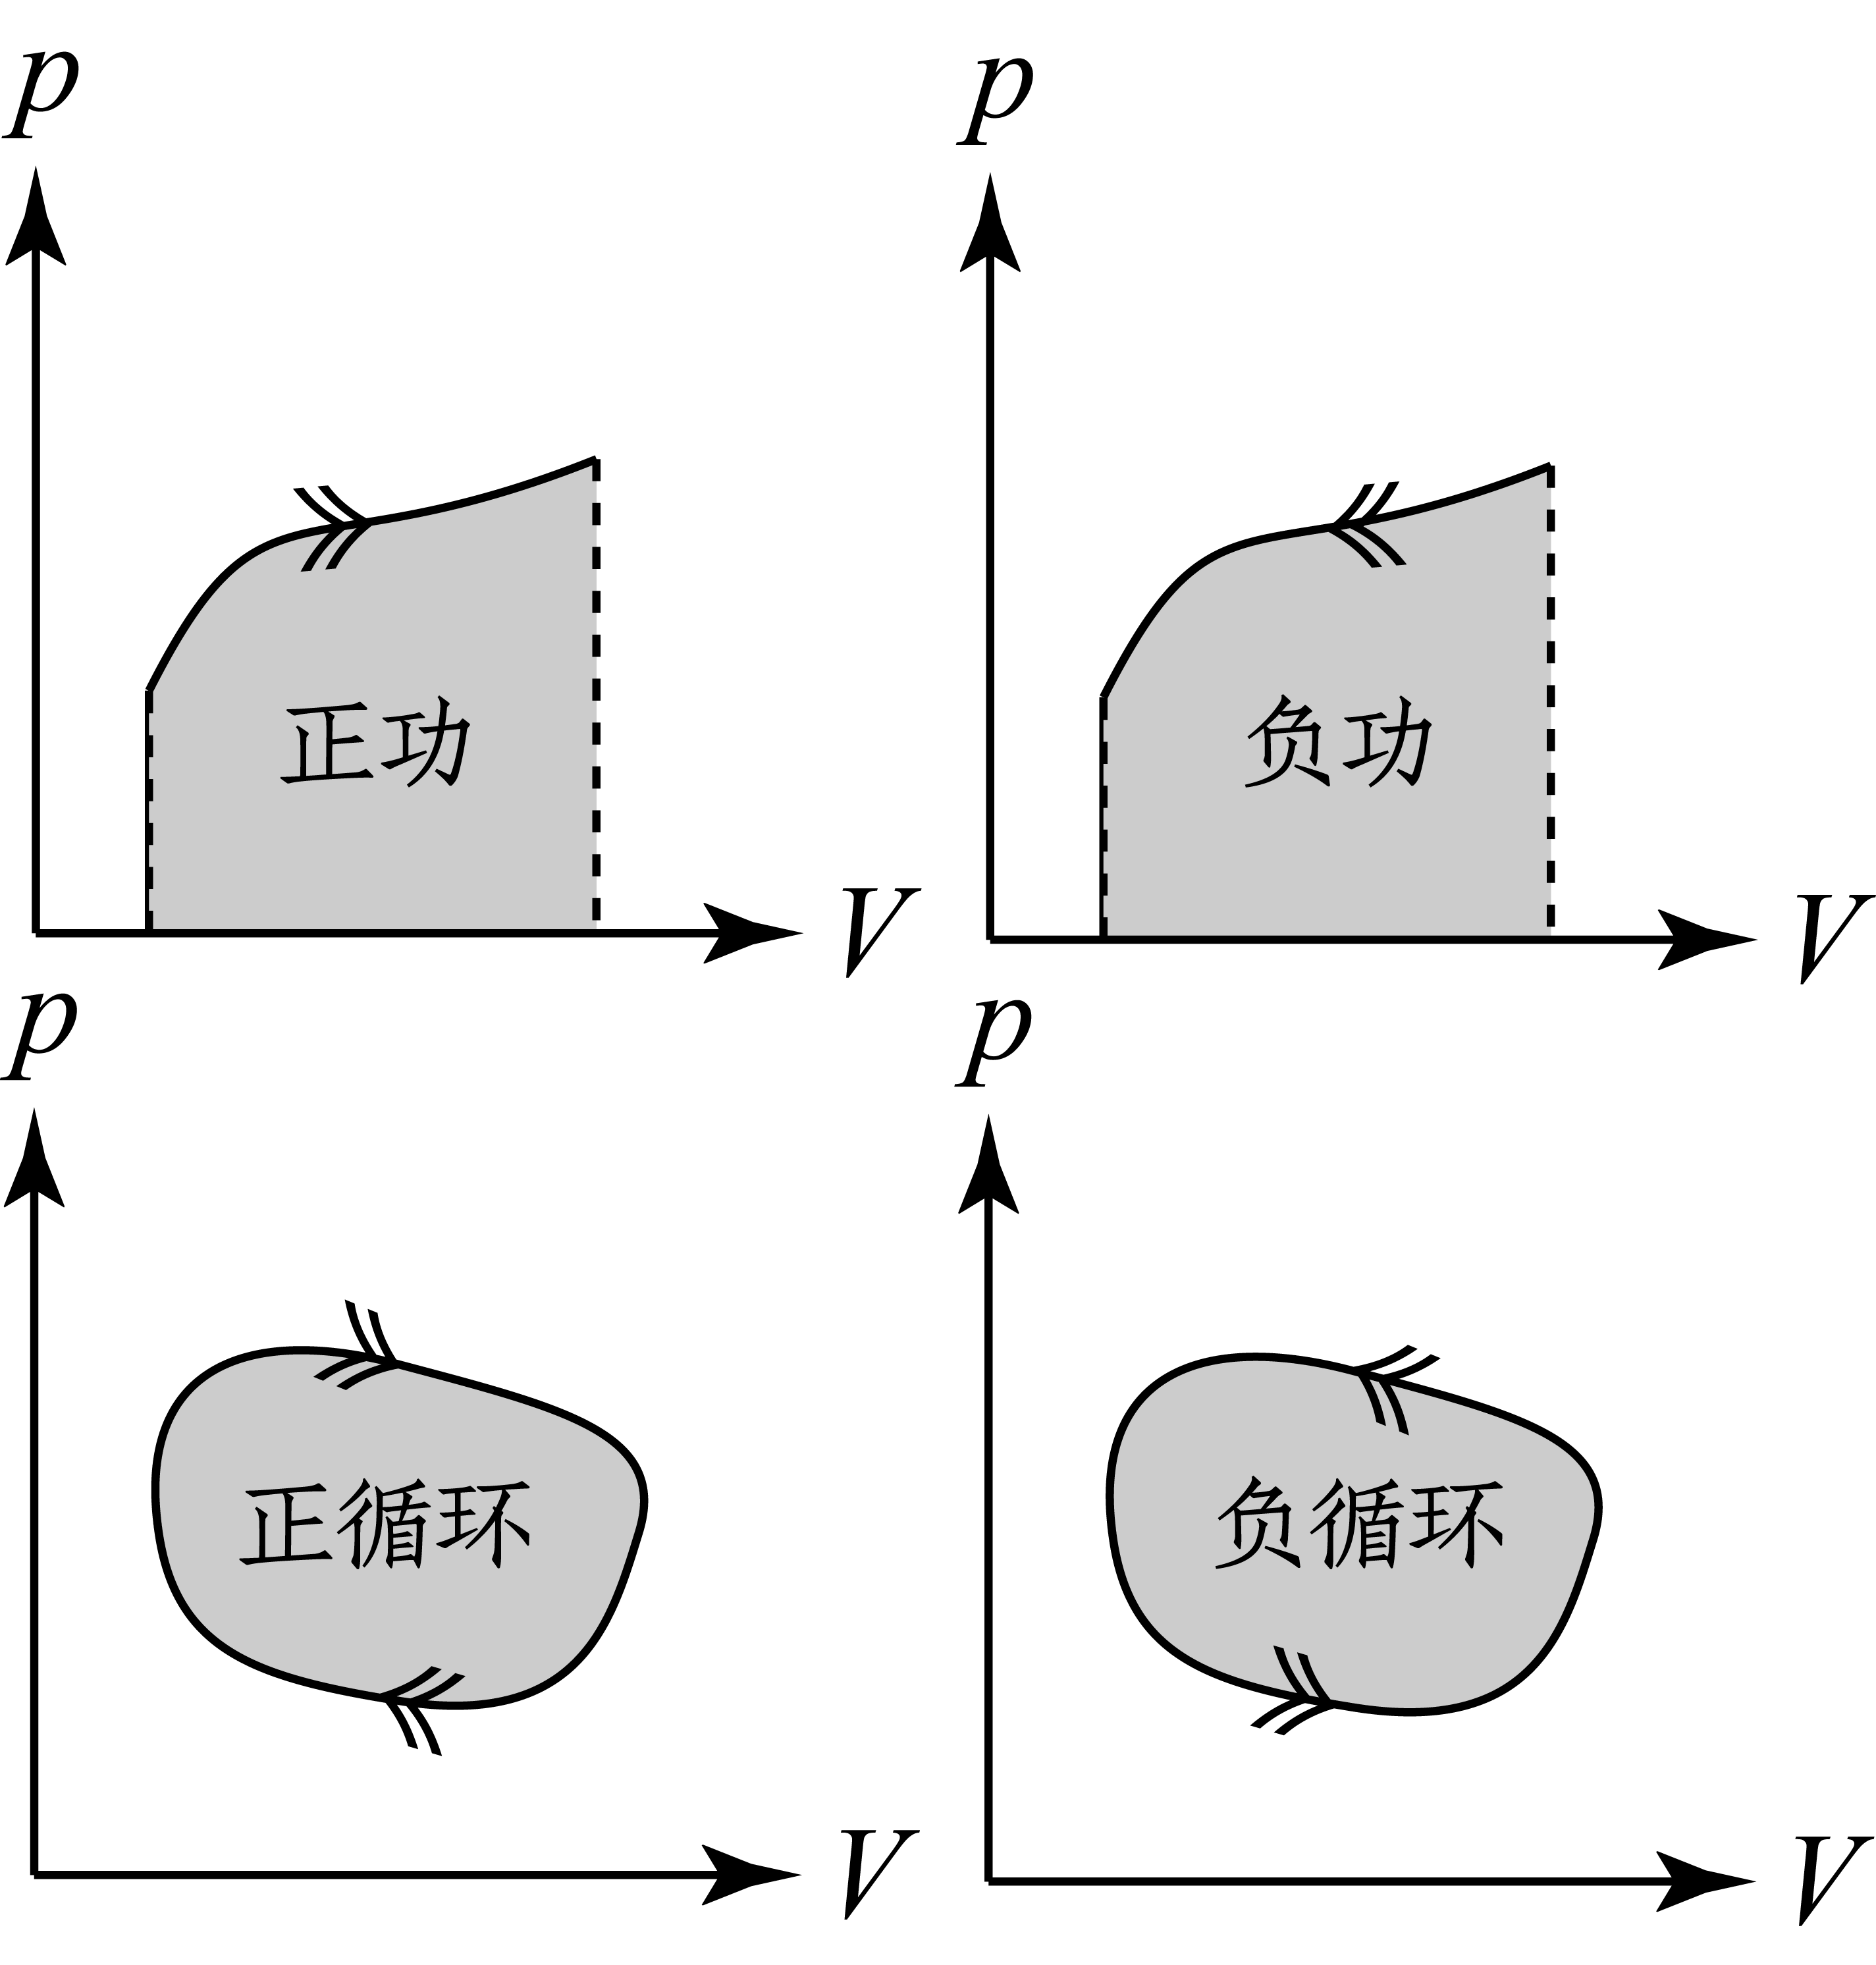
\includegraphics[width=7cm]{image/5-1-1.png}
\caption{准静态过程的做功}
\end{wrapfigure}
对于体积功,\,在准静态过程中可以由$p-V$图下的面积计算.\,在循环过程中则等于过程曲线所包含的面积.\,注意其正负号与过程方向之间的关系.\,但对于非准静态过程.\,做功一定要由外界参数(活塞加速度,\,活塞外气压等)计算而不是用内部气体的过程方程.\,这是因为即使形式地写出内部气体所发生的过程的过程方程.\,由于气体发生膨胀处的压强不等于过程方程中的平均压强,\,对做功的计算是没有意义的.
\subsection{热量}
做功与\emph{传热}(heat transfer)是截然不同的两种向系统注入能量的方式.\,做功依赖于广义坐标这一参数的改变.\,本质上与每一个微观粒子的能量对于广义坐标的依赖有关.\,然而热量则完全不依赖于外在的参数.\,它与系统粒子关于不同能量的状态的占据数\emph{配分}(partition)有关.\,也就是与温度息息相关.\,温度高的物体,\,占据在高能量状态上的粒子较多,\,低能量状态的粒子较少,\,与低温物体发生热接触时,\,单位时间内高能粒子碰撞低能粒子传递能量的可能性更高.\,其统计平均效应就是高温物体向低温物体放热.\,准静态的\emph{等温传热}又是怎样一个过程呢?\,从以上分析可知,\,产生温度梯度是有热传导\footnote{注意,\,广义的热量传递还包括热对流与热辐射.}的必要条件,\,没有了温度差热量的交换也就无从谈起了.\,从这个意义上说,\,实际发生的过程其实都是非准静态过程,\,准静态过程仅仅是一种实际过程的一种近似.\,或是我们虚设的一种模型.\,如在等温传热模型中,\,我们设想只让一个物体的高能粒子与另一个物体的低能粒子发生热接触而实现热传递,\,这无疑会破坏热力学的统计规律\footnote{或是借助于所谓的麦克斯韦妖,\,引入信息熵.},\,但有助于我们理解这个过程的发生机理.

\npg{-10pt}

\subsection{耗散}
\begin{wrapfigure}[14]{o}[-10pt]{7cm}
\centering
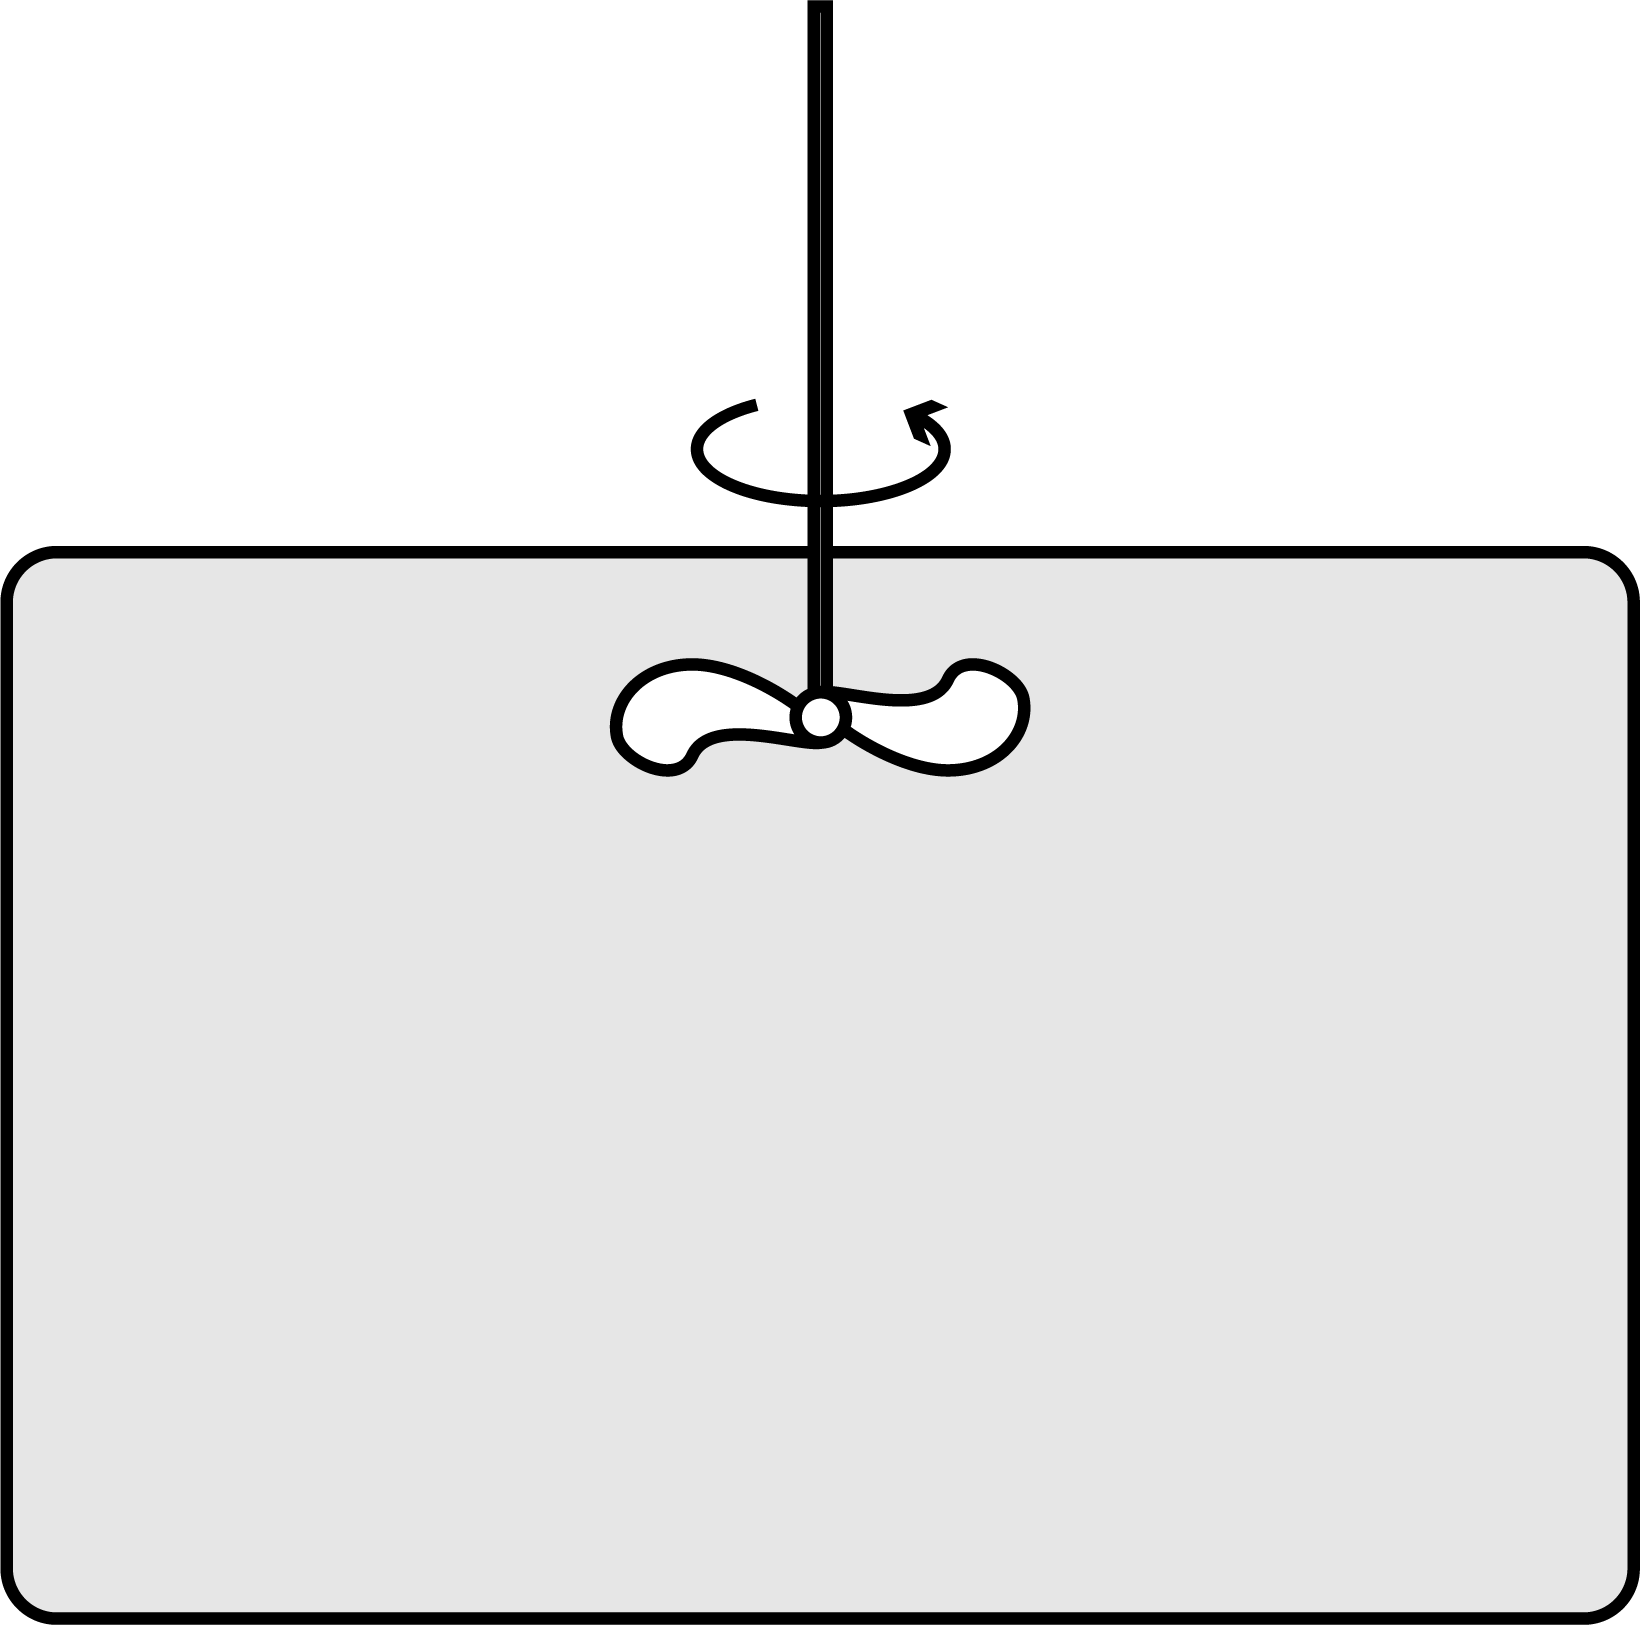
\includegraphics[width=6cm]{image/5-1-2.png}
\caption{搅动空气发热}\label{fig:1-2}
\end{wrapfigure}
还有一类向系统输送能量的方式,\,表面上看是功,\,效果上却是热.\,这被我们称为\emph{耗散}(dissipation).\,俗称\emph{功变热}.\,例如常见的摩擦生热过程,\,非弹性碰撞的过程,\,激光泵浦的过程.\,都是典型的功变热的例子.\,我们看一个十分浅显的例子.\,涡轮叶片搅动气缸中的空气使其温度升高.\,在这个过程中,\,涡轮无疑对气体做功,\,但这个做功并不与系统广义坐标的变化相关.\,它的特点是仅仅作用在系统的一个子系统上.\,再由系统倾向于热平衡的趋势把得来的能量平分到系统各个自由度上.\,从而造成了与吸热完全类似的结果:\,广义坐标没有变化,\,但系统从外界获得了能量.

究其原因,\,本质上是因为系统具有了所谓的\emph{耗散结构}(dissipative structure).\,它不把系统看成一个平衡的整体,\,而是有着复杂内部非线性相互作用的对象.\,故输入的功不一定改变体系的广义坐标,\,但像加热一个系统一般,\,增加了系统的内能.

耗散结构的特点之一是外力驱动系统远离平衡态.\,在非弹性的碰撞过程中固体内部的低频弹性波的成分被突然增强,\,而激光发射的过程中大量粒子被输运到亚稳态而实现布居反转,\,这些都破坏了原来热平衡下的布局.\,需要结合动力学与统计方法来讨论这些现象.

特点之二是开放条件下的自组织现象.\,以普利高津({\it Progogine})为首的研究者把生命现象,\,连同研究过程中的很多奇特现象看成是一种耗散结构的结果.\,这些过程伴随着系统与外界连续不断的能量,\,粒子与信息的交换,\,使得微小的涨落可以在具有正反馈的功能结构中被放大,\,使得体系的对称性被破坏,\,形成有组织的自发序.
\begin{figure}[H]
\centering
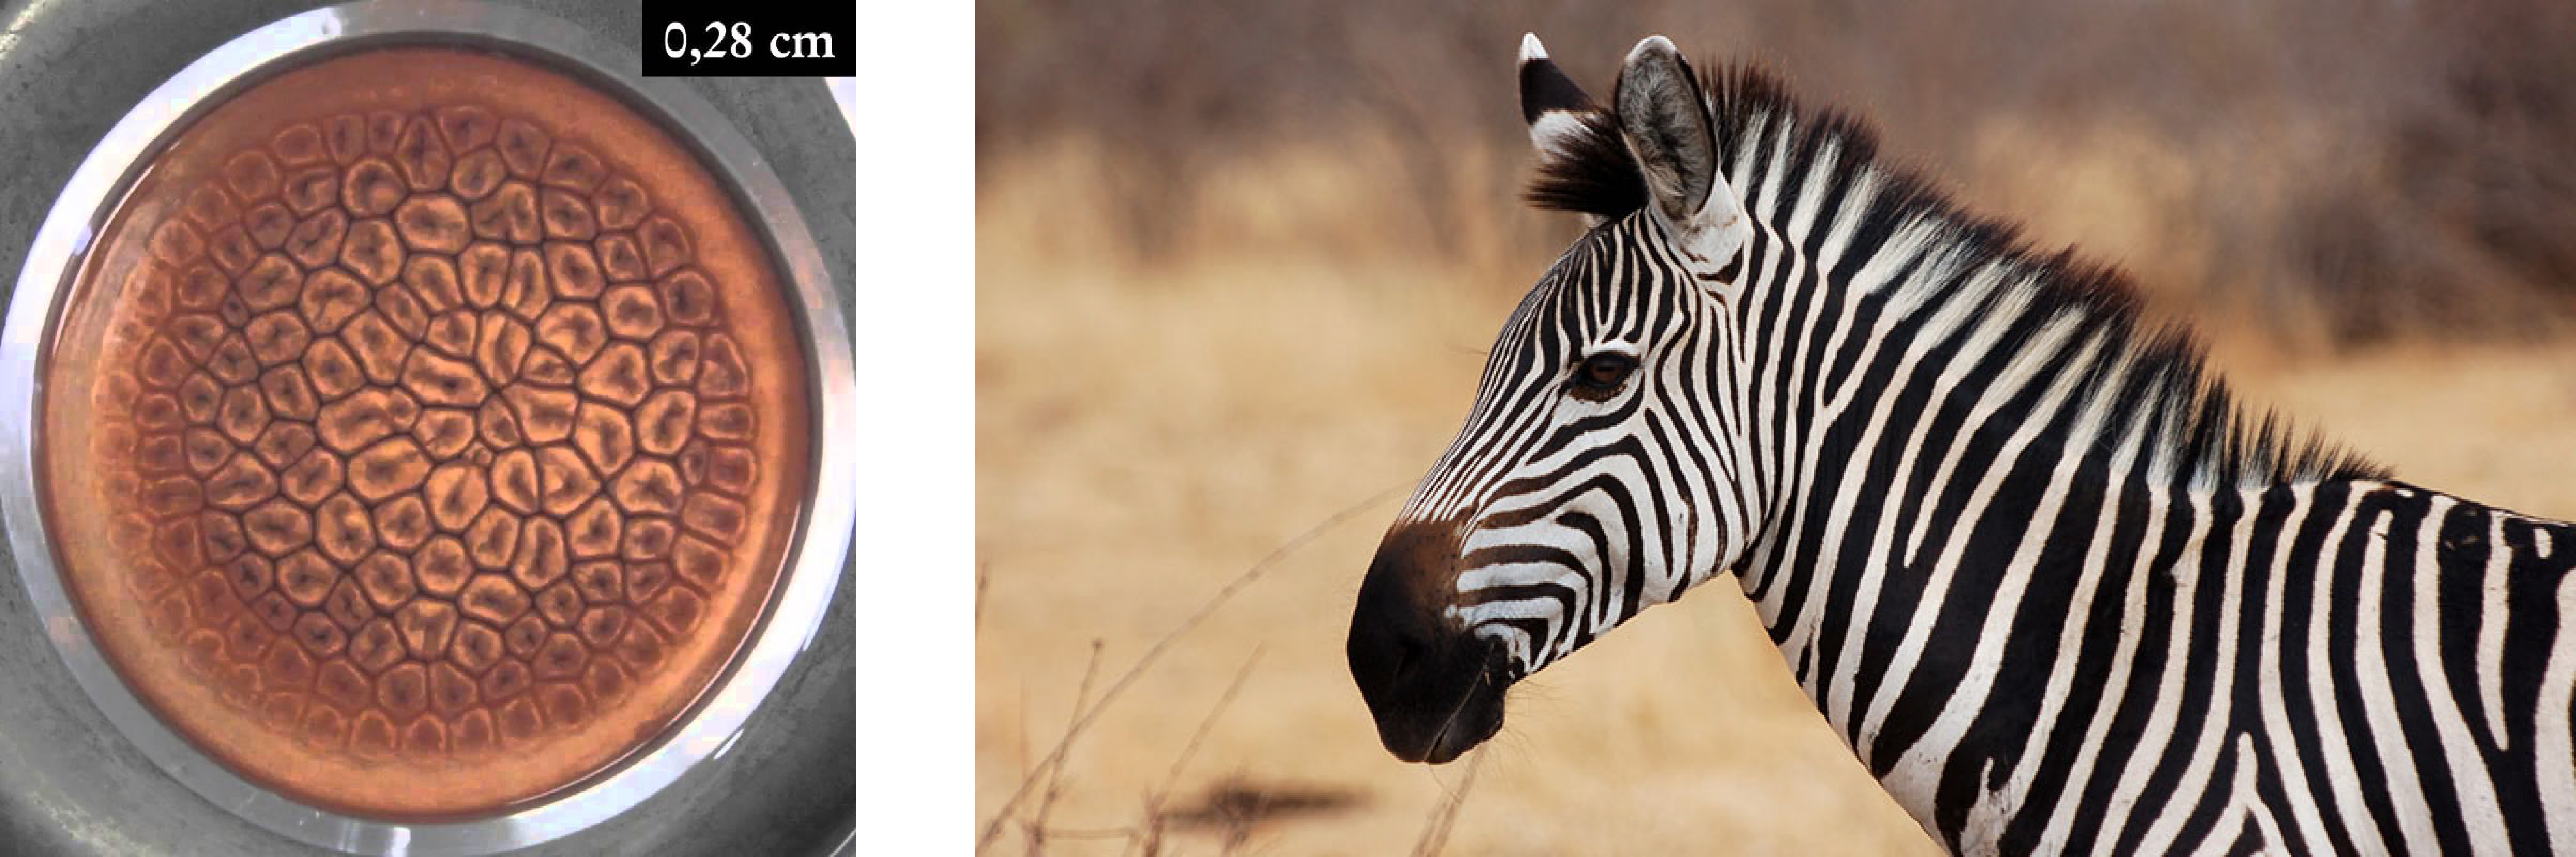
\includegraphics[width=14cm]{image/5-1-3.png}
\caption{自组织现象:\,B\'enard 对流与斑马身上的条纹}
\end{figure}


\npg{-10pt}

\section{理想气体}

\subsection{理想气体的定义}

满足以下三个条件的气体为理想气体:
\begin{enumerate}
	\item 分子间作用力可以忽略;
	\item 分子体积可以忽略;
	\item 分子按自由度平分能量.
\end{enumerate}

我们讨论一下这三个条件.\,首先第一个条件的意思,\,旨在把理想气体间的作用力当成\emph{短程力}(short-range force)处理.\,仅仅当两个分子间距离进入力程范围才可以当做可以发生相互作用(碰撞或散射).\,在这个意义下,\,分子体积实际上也可以处理为半径为力程大小的钢球模型.\,我们忽略这一个体积,\,也就是说所有分子可以自由活动的体积就等于容器体积$V$.\,且分子间相互作用力为零.

然而这两点合在一起将导致一个严重的问题:\,那便是热平衡不可以达到.\,若每个分子不可以通过相互作用或刚性的碰撞与别的分子交换能量与动量.\,那从根本上就不可以达到热平衡,\,统计方法也就无济于事.\,故分子体积足够小,\,小到可以忽略其对热力学性质的影响,\,但又足够大,\,大到在我们关心的时间空间尺度内体系能很快地达到热平衡.\,这才是对这两点的正确理解方式.

我们设分子的速率分布函数为$f(v)$,\,意思是每取$N$个分子,\,速率介于$v$到$v+\ud v$的分子数平均为:
\[\ud N=Nf(v)\ud v\]

从而分子的平均速率与方均速率为:
\[\overline{v}=\int_0^\infty vf(v)\ud v \quad ; \quad \overline{v^2}=\int_0^\infty v^2 f(v)\ud v\]

分子质量为$m$,\,直径为$D$,\,数密度为$n$.\,从中我们得出分子间平均距离$d$:
\[d\sim\frac{1}{\sqrt[3]{n}}\]

\begin{wrapfigure}[15]{o}[-10pt]{7cm}
\centering
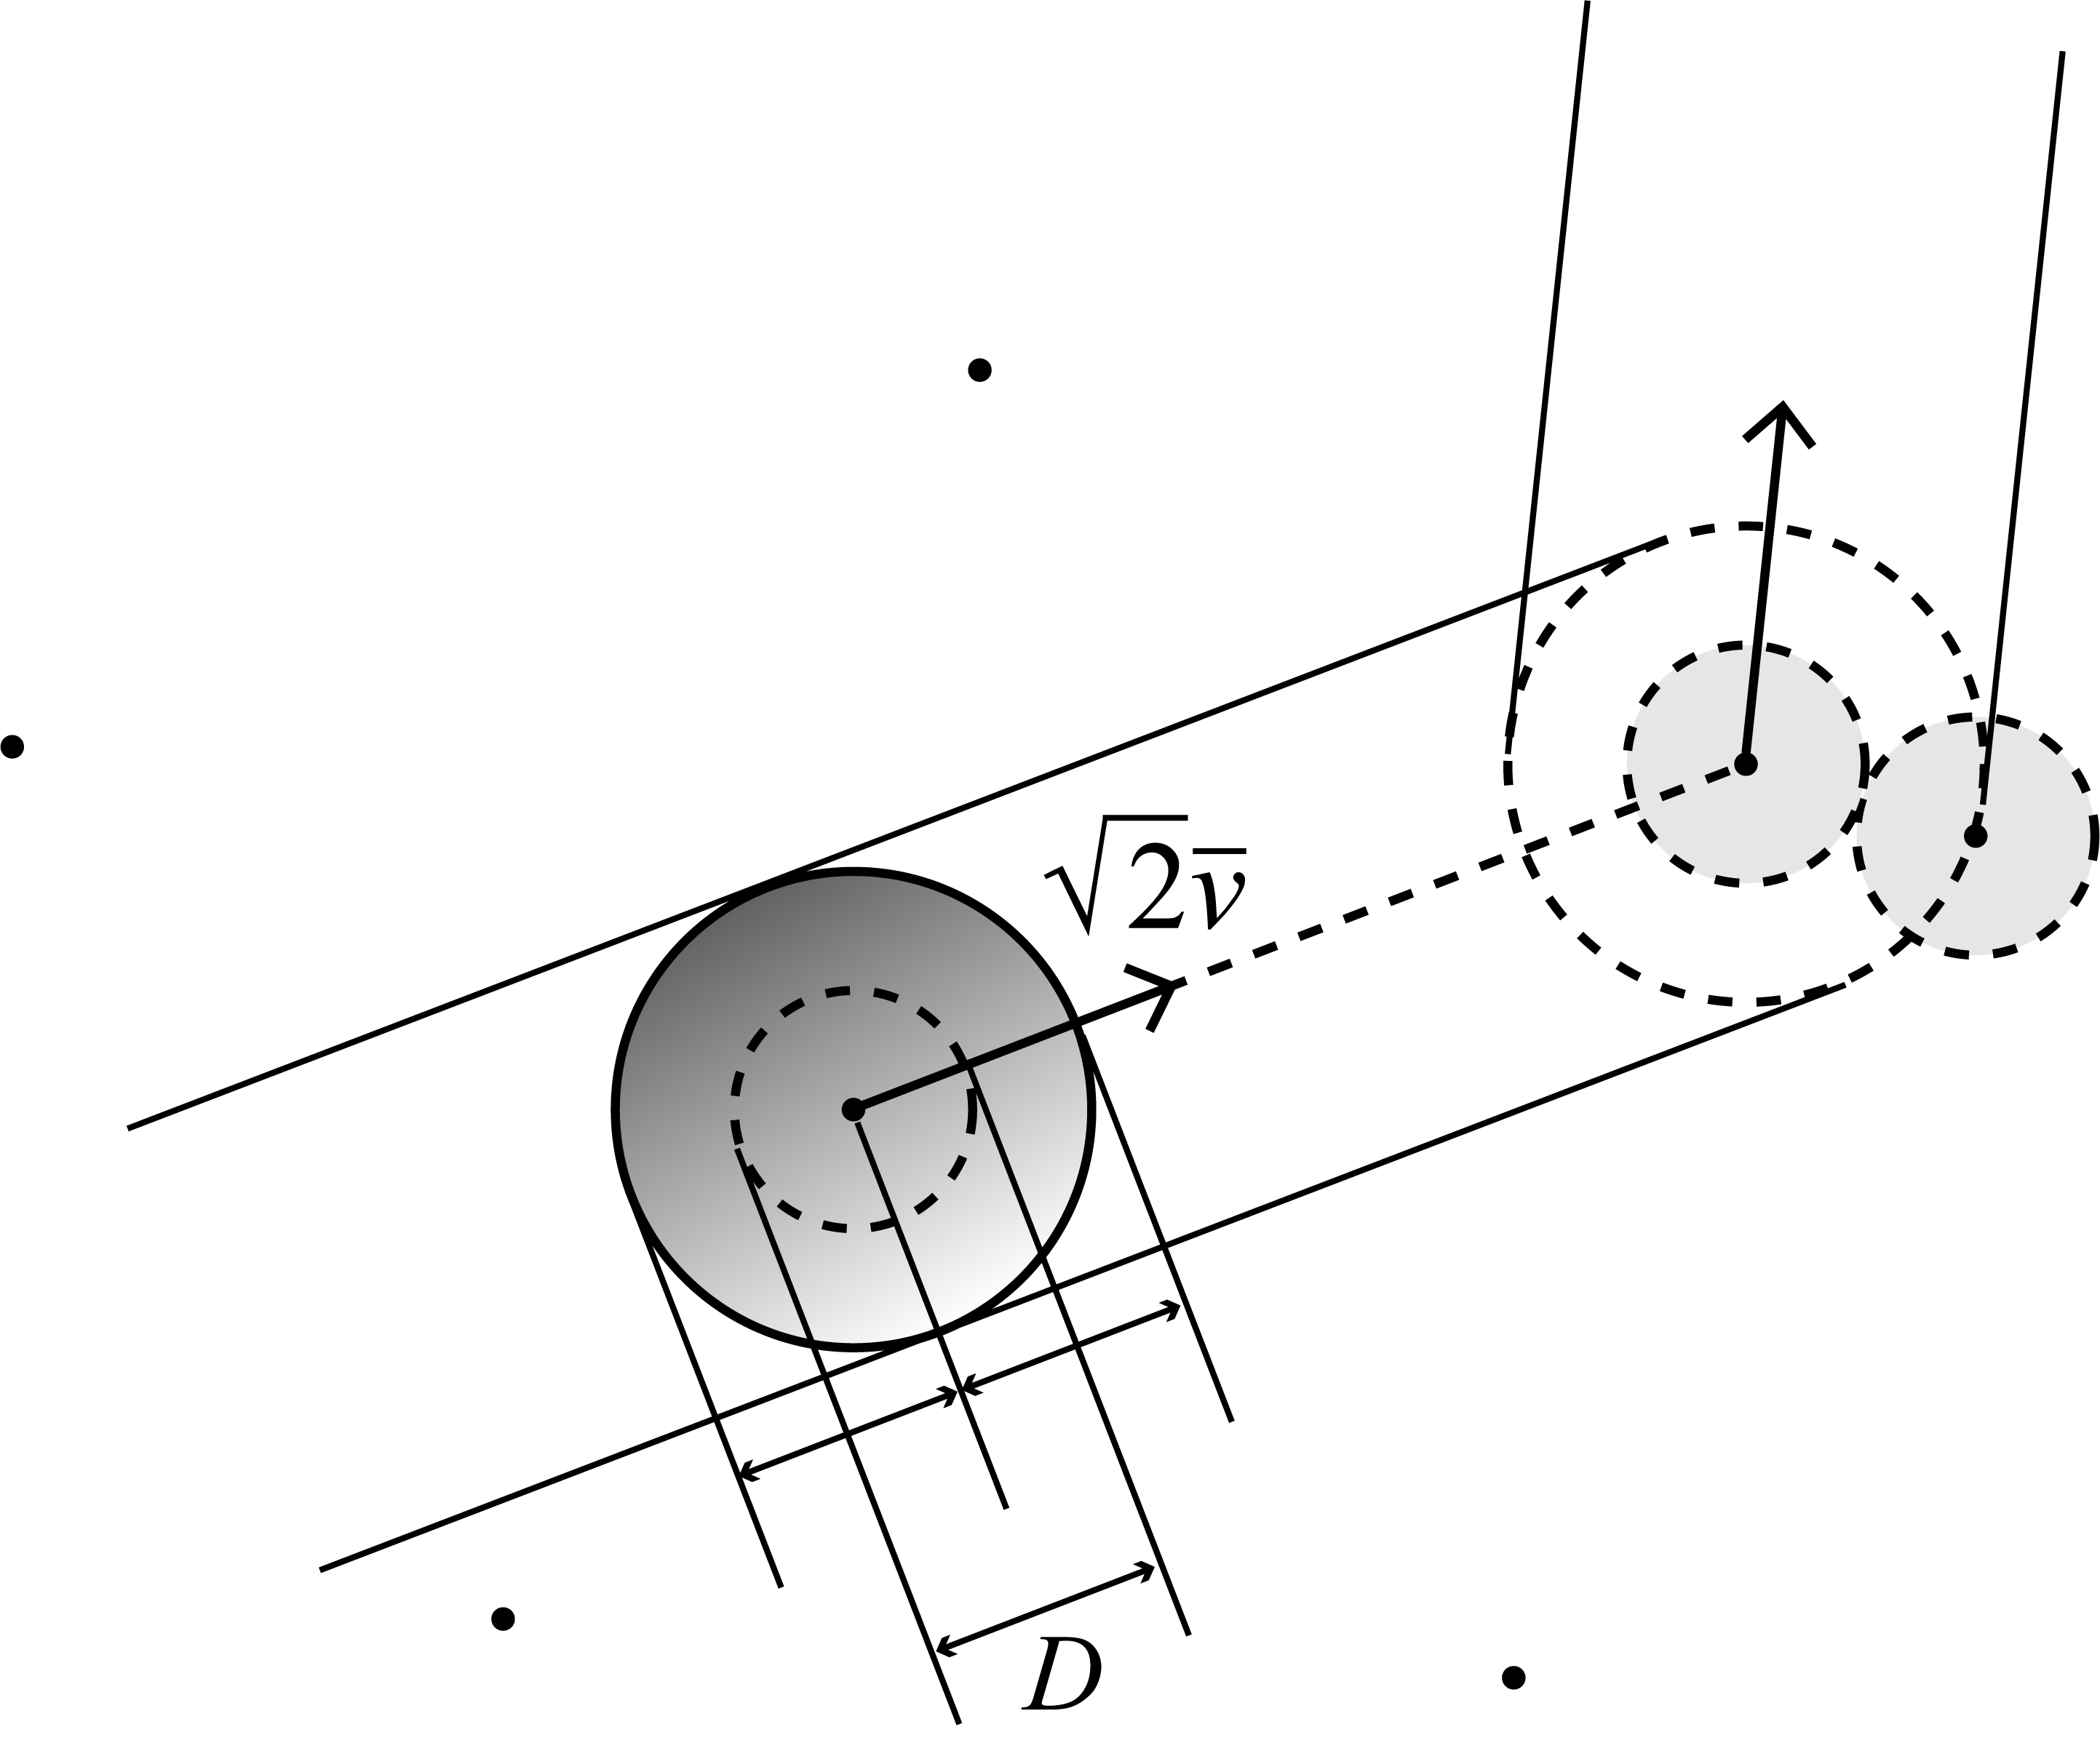
\includegraphics[width=6cm]{image/5-1-4.png}
\caption{曲折柱体计算}
\end{wrapfigure}
可以想见,\,分子间平均距离$d\sim 10{\rm nm}$(大气压下)越大,\,分子直径$D\sim 1{\rm nm}$越小,\,气体越能够近似为理想气体.\,同时其相隔两次碰撞的平均时间间隔$\tau$与空间间隔$\lambda$也会越大.\,如何计算这两个量呢?\,由于分子的速度符合麦克斯韦分布律(参见第五章),\,故两分子间的平均相对速率为$\sqrt{2}\overline{v}$.\,将待研究的粒子处理为钢球,\,速率恒定为$\sqrt{2}\overline{v}$,\,其半径为原分子直径$D$.而其他分子处理为静止的质点,\,半径为零.\,这样钢球碰到质点,\,即相当于原来的两个分子发生碰撞.\,而时间$t$内钢球扫过的体积为:
\[V(t)=\pi D^2\cdot \sqrt{2}\overline{v}t\]

发生碰撞次数$c$:
\[c(t)=nV(t)\]

当$c=1$时,\,对应的时间即为平均自由时间$\tau$,\,又称为\emph{驰豫时间}(relaxation time),\,而这一段时间内粒子走过的距离即为\emph{平均自由程}$\lambda$(mean free path):
\[\tau=\frac{1}{\sqrt{2}\pi nD^2\overline{v}} \quad ; \quad \lambda=\frac{1}{\sqrt{2}\pi nD^2}\]

即有:
\[\lambda\sim\frac{d^3}{D^2}\sim 100d\sim 1{\rm \upmu m}\]

以上数据仅仅在大气压下有效,\,注意平均自由程与分子平均速度无关,\,仅仅是一个几何相关量.\,而它与$n$成反比,\,也就是与$p$成反比,\,如果压强减小到约$1{\rm Pa}$(而温度不变),\,则平均自由程$\lambda$增大5个量级,\,也就是分米量级.

现在我们做一个总结:\,我们取了一个分子间相互作用力与分子的大小可以忽略的模型来研究理想气体,\,它对应的条件是:
\[D \ll d \quad ; \quad \lambda\sim\frac{d^3}{D^2} \ll L\]

第一个条件是保证分子体积可以忽略,\,第二个条件是在研究的问题尺度内保证分子有足够的空间来实现动量能量交换以达到热平衡.

现在让我们专心研究第三个条件.\,能量按自由度均分是麦克斯韦分布的一个独特结果.\,详情也可以参见第五章.\,现在我们指出,\,由于系统中的各个自由度,\,如$x,\,y,\,z$方向的平动,\,分子的转动,\,振动的能量具有相似的形式\footnote{指谐振子形式,\,详见第五章.},\,而且可以通过相互作用(碰撞)交换能量,\,总能量守恒.\,在这样的条件下,\,统计规律告诉我们每一个分子每一个自由度上都分得相同的平均能量值.\,这个平均能量值\footnote{及其对应的按能量高低的配分.}即代表了体系的温度:
\[\overline{\varepsilon}=\frac{1}{2}kT\]

体系自由度越多,\,分子数越多,\,在一定温度下储能就越多:
\[U=N\cdot\frac{f}{2}kT\]

其中$f$是系统能量自由度数\footnote{注意其与动力学自由度的区别,\,振动的势能也对应能量自由度,\,但其动力学自由度与振动动能重合.}.\,它被视为与温度无关的常量\footnote{然而实验发现这些不是常量,\,而是随着温度升高越来越大,\,存在一些基本不变的平台,\,思考这意味着什么.}.\,对于上式,\,我们再引入\emph{摩尔}(mole)这一化学计量单位来表示巨大的原子数$N$:
\[\frac{N}{N_A}=\nu \quad ; \quad N_A=6.022140857\pow{23}/{\rm mol}\]

同时,\,普适气体常量被定义为:
\[R=N_A k=8.314{\rm J/mol\cdot K}\]

这样气体的内能即为:
\[U=\frac{f}{2}\nu RT\]

\subsection{理想气体物态方程}
我们发现,\,$\ud p_1=f(v)\ud v$表示的含义为任意一个分子的速率落在$v\sim v+\ud v$区间内的概率.\,然而对于这样的分子,\,它速度方向在空间中的取向是任意的,\,各向同性的.\,所以建立极轴后,\,速度与极轴夹角在$\theta\sim\theta+\ud \theta$范围内的概率又为:
\[\ud p_2=\frac{\ud \Omega}{4\pi}=\frac{2\pi\sin\theta\ud\theta}{4\pi}=\frac{\sin\theta\ud\theta}{2}\]

对于这样的分子,\,它在容器中的任何位置都是有可能且等概率的,\,所以出现在体积微元$\ud V$中的概率还有$\ud p_3$,\,联合概率为$\ud p=\ud p_1\ud p_2\ud p_3$.

\begin{wrapfigure}[12]{o}[-10pt]{6cm}
\centering
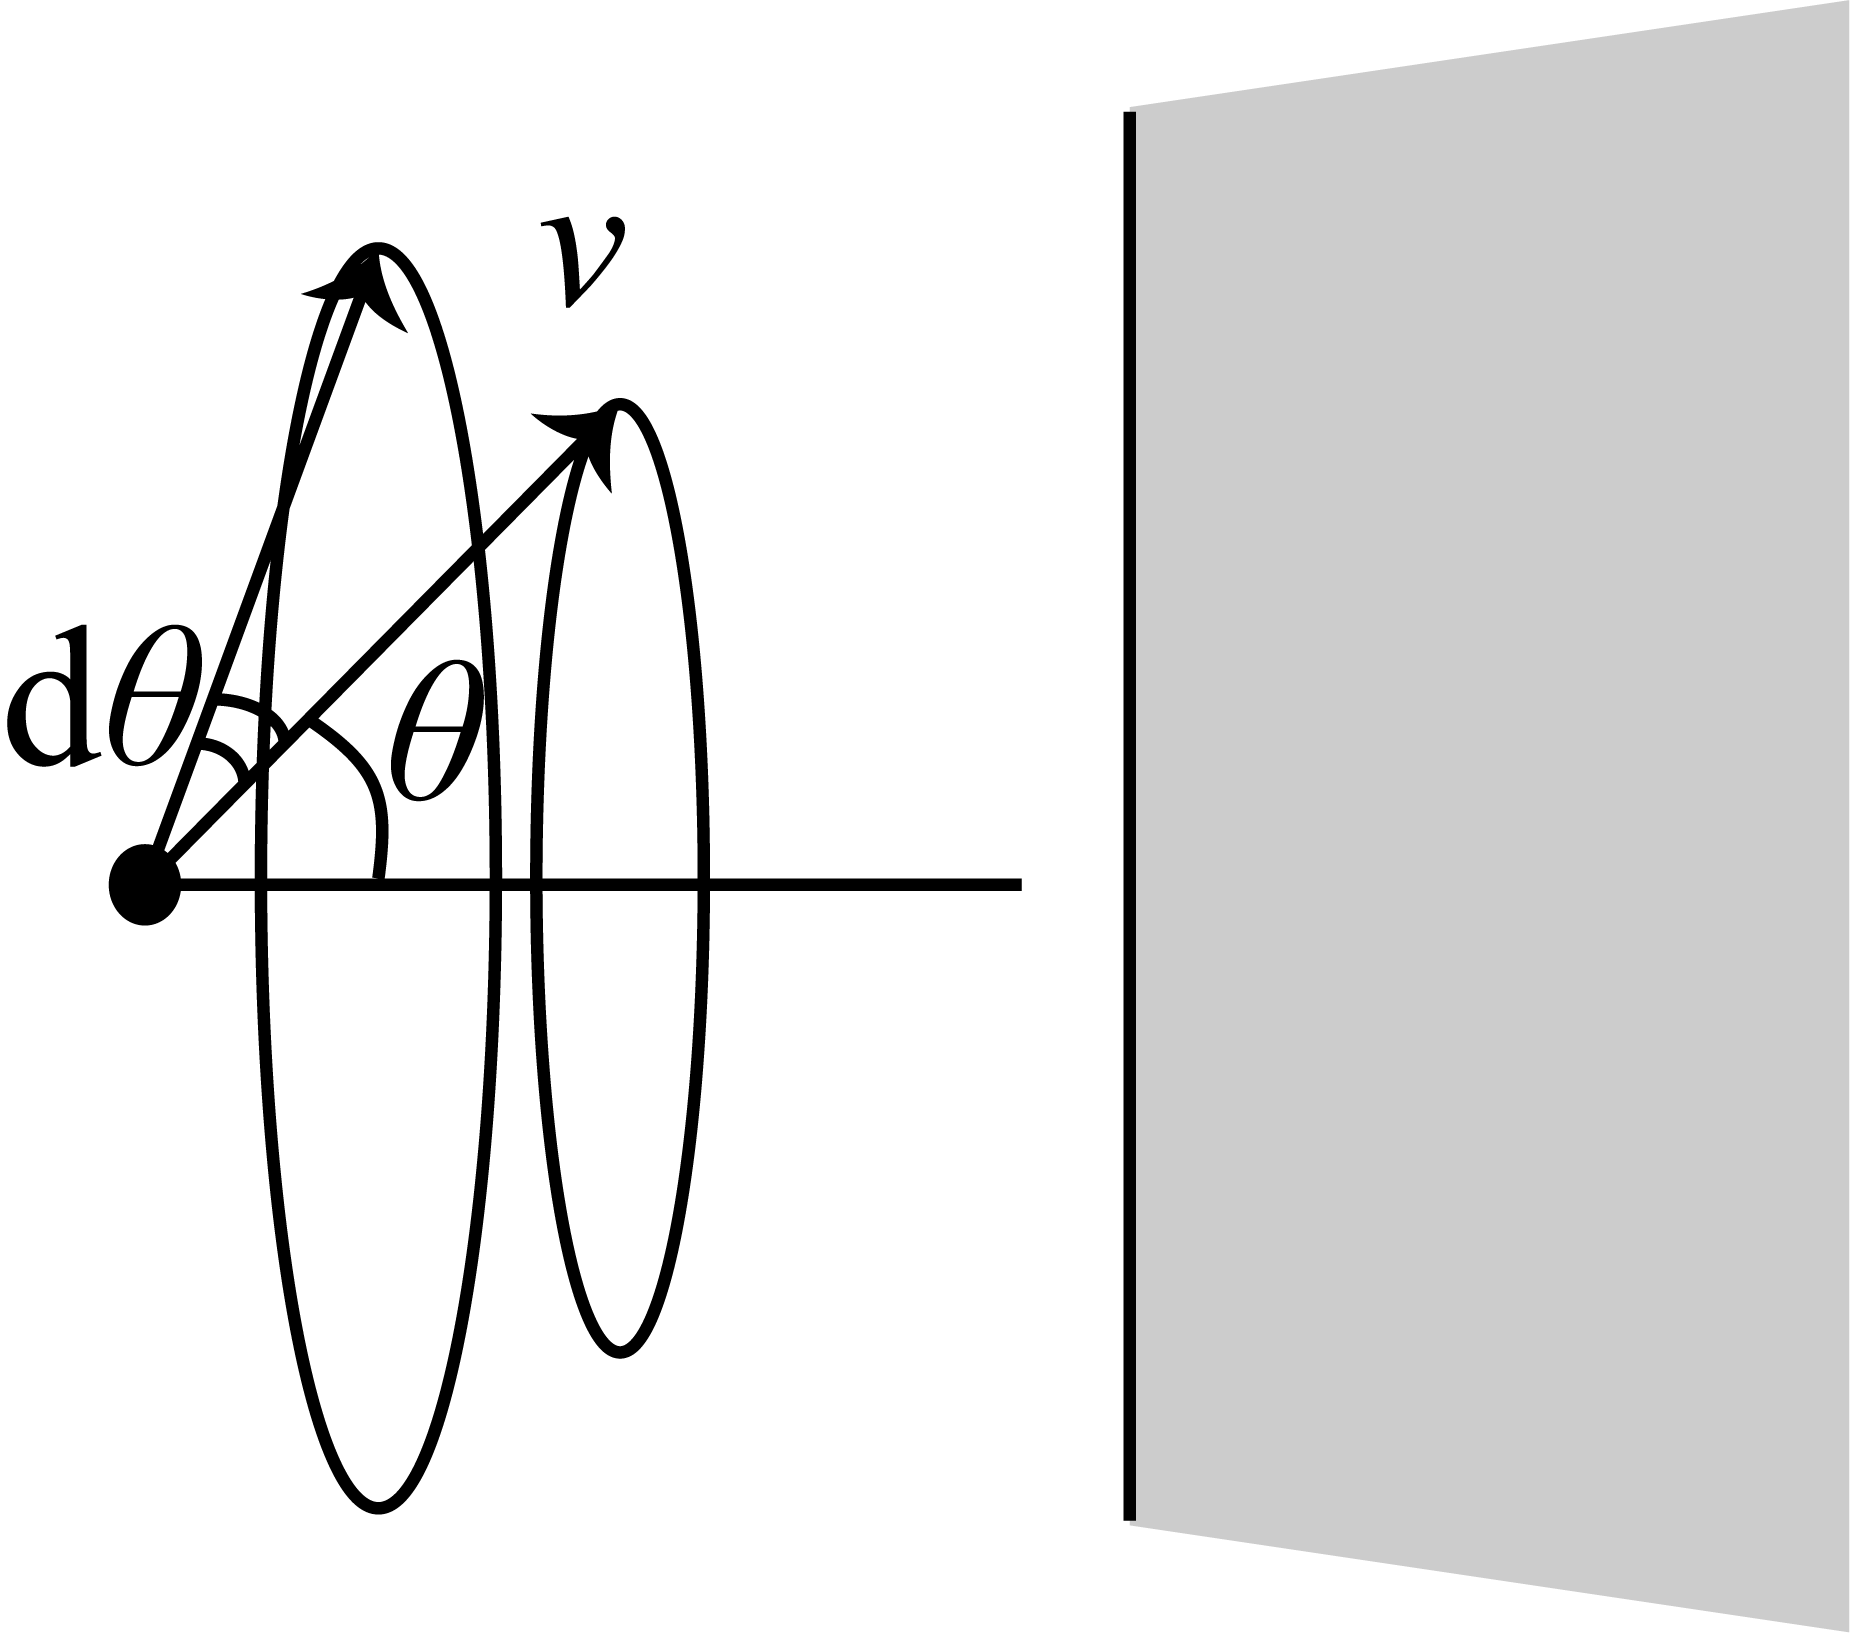
\includegraphics[width=6cm]{image/5-1-5.png}
\caption{粒子速度方向分布}
\end{wrapfigure}
我们接下来考虑气体的压强.\,在这之前我们了解两个概念是十分有帮助的:\,处于平衡态的系统可以看成互相达到平衡的各部分\emph{子系统}(subsystem)直接组成.\,这些部分的所有\emph{强度量}(intensive property)都是完全一致的,\,如理想气体的压强,\,温度,\,粒子数密度,\,摩尔体积,\,摩尔内能等等.\,而子系统的\emph{广延量}(extensive property)大小之和即为总系统的对应量的大小,\,如分子数,\,摩尔数,\,体积,\,内能,\,焓等等.\,我们可以这么理解:\,强度量描述体系的内禀属性,\,而广延量仅仅反应全同子系统的简单堆积.\,如一杯盐水,\,确定了我们关心的强度量\ca 温度和浓度之后,\,我们就可以回答``怎样的盐水''这一个问题.\,而接下来只需要再回答``有多少''这一个简单的问题,\,就能算出所有的广延量来.\,基于这一点理解,\,我们可以发现以下两个性质是成立的:\\[1pt]

{\hei 保持所有强度量不变,\,一个广延量变化$\lambda$倍,\,所有广延量随之变化$\lambda$倍.}\\[1pt]

{\hei 两个广延量之比为强度量,\,典型的如质量$M$比体积$V$为密度$\rho$,\,体积$V$比摩尔数$\nu$为摩尔体积$v$等.}\\[1pt]

理想气体作为极其简单的系统,\,它的独立强度量仅仅只有两个.\,一是系统的温度$T$.\,它决定了分子的平均热运动剧烈程度,\,也就是平均能量大小.\,另一个就是分子数密度$n$,\,它反映单位体积里有多少个全同单元,\,是一种``浓度''.\,其他所有强度量都是这两个量的导出.\,比如压强$p$,\,用分子动理论的方法:
\begin{eqnarray*}
p 	&=&	\int_0^{\infty}\int_0^{\frac{\pi}{2}}n\ud S v\cos\theta\ud t \cdot f(v)\ud v \cdot\frac{\sin\theta\ud\theta}{2}\cdot 2mv\cos\theta/\ud S\ud t 	\\
	&=&	nm\cdot\int_0^{\infty}v^2 f(v)\ud v \cdot \int_0^{\frac{\pi}{2}}\sin\theta\cos^2\theta\ud\theta	\\
	&=& \frac{1}{3}nm\overline{v^2}		\\
	&=& \frac{2}{3}n\overline{\varepsilon_k}	\\
	&=& nkT
\end{eqnarray*}

可见对容器壁的压强正比于温度和分子数密度,\,这一点的物理图像还是很直观的.\,这个压强被我们称之为\emph{外压强}(outer pressure).\,它是由于分子碰撞容器壁引起.\,还有所谓的\emph{内压强}(inner pressure)的概念,\,它由于分子间的碰撞引起.\,理想气体的内压强与外压强相等\footnote{然而范德瓦尔斯气体则不然,\,详见第四章.}.\,但如果气体足够稀薄,\,以至于容器尺度与分子平均自由程可以比拟.\,此时内压强的概念也失去了意义,\,这意味着气体完全不可以用动力学方法处理,\,压强的梯度不会导致气体团的加速度,\,而是以下面所介绍的泻流的方式进行.

上文我们推出来的关系式被称作(强度量之间的)\emph{物态方程}(equation of state),\,它有很多变式,\,如:
\[pV=NkT \quad ; \quad pV=\nu RT \quad ; \quad pv=RT \quad ; \quad p=\frac{\rho RT}{\mu}\]

上面最后一式中$\mu$表示摩尔质量,\,稍作变形还可以得到密度公式:
\[\rho=\frac{\mu p}{RT}\]

用分子动理论方法还可以得到另一个十分重要的量\ca \emph{泻流数}(effusion number).\,如果在容器壁上开一个小孔.\,则速率在在$v$到$v+\ud v$区间内的分子,\,单位面积单位时间通过小孔的分子数为:
\begin{eqnarray*}
\ud \Gamma 		&=& 	\int_0^{\frac{\pi}{2}}n\ud S v\cos\theta\ud t \cdot f(v)\ud v \cdot\frac{\sin\theta\ud\theta}{2}/\ud S\ud t 	\\
				&=&		\frac{n}{2}\cdot \int_0^{\frac{\pi}{2}}\sin\theta\cos\theta\ud\theta	\\
				&=&		\frac{1}{4} nv f(v)\ud v 	\\
				&=&		\frac{1}{4}\ud n v
\end{eqnarray*}
可见速率为$v$的那一部分分子,\,泻流数就是$\ud \Gamma=\frac{1}{4} \ud nv$.\,那么对于所有分子,\,总泻流数为:
\[\Gamma=\frac{1}{4}n\overline{v}\]

泻流的条件是开的孔的大小足够小,\,以至于分子在穿过孔时不会受到别的分子的碰撞.\,也就是其平均自由程$\lambda$显著地大于孔的直径$L$.\,相反地,\,如果$\lambda\ll L$,\,那么就变成了一种压强差驱动气体集团运动的动力学模型,\,我们在下一节阐述.

最后,\,理想气体的内能则可以根据之前关于温度定义的讨论,\,直接写出:
\[U=\nu C_{mV} T\]

其中$C_{mV}$被称为\emph{定容摩尔热容}(molar heat capacity at constant volume).\,其意义之后将了解.\,现在只需知道$\displaystyle C_{mV}=\frac{f}{2}R$.

\subsection{混合理想气体}
考虑几种理想气体的混合,\,我们也需要忽略几种组分分子间的相互作用,\,尤其是应该排除几种分子间发生化学反应的情况\footnote{如混合{$\rm NH_3$}与{$\rm Cl_2$}.}.\,此时,\,几种气体由各自的数密度$n_i$和热平衡下的公共温度$T$描述.\,另一种描述方法是给出总分子数密度$n$与各组分分子所占的比例(强度量)$x_i$:
\[n=\sum n_i \quad ; \quad x_i=\frac{n_i}{n}\]

称为\emph{摩尔分数}(mole fraction),\,注意$x_i$间要满足的归一关系:
\[\sum x_i=1\]

不同组分间分子纵然有碰撞,\,但这对于这一部分分子碰撞容器壁产生的压强大小没有影响.\,也就是说,\,压强等于各组分以$n_i$单独存在时对容器壁产生的分压$p_i$.\,这叫做\emph{道尔顿分压定律}({\it Dalton}'s law of partial pressures):
\[p=\sum p_i \quad ;\quad p_i=n_i kT=x_i p \quad ; \quad p=nkT\]

值得注意,\,每个分子的质量$m_i$或能量自由度数$i_i$并不影响压强的计算.\,压强单方面地决定于分子数密度与温度(分子平均平动动能.\,分子质量改变的是整个体系的摩尔质量$\mu$,\,取一定体积的气体:
\[M=\nu\mu=\sum M_i=\sum \nu_i\mu_i \quad \Rightarrow \quad \mu=\sum x_i \mu_i\]

其中出现的摩尔数$\nu_i$之比即为分子数密度$n_i$之比,\,而摩尔质量$\mu_i$与分子质量的换算关系也很基础,\,请读者一定要熟练使用:
\[\nu_i : \nu_j=\frac{n_i V}{N_A} : \frac{n_j V}{N_A}=n_i : n_j \quad ; \quad \mu_i=N_A m_i\]

能量自由度数影响的是摩尔内能$u$:
\[u=\nu \overline{C_{mV}} T=\sum u_i=\sum \nu_i C_{mVi} T \quad \Rightarrow \quad \overline{C_{mV}}=\sum x_i C_{mVi}=\sum \frac{x_i f_i}{2}R\]

上面我们定义了平均摩尔定容热容$\overline{C_{mV}}$.\,平均的含义一定是按分子数$n_i$(摩尔数$\nu_i$,\,比例$x_i$)平均.

\subsection{理想气体的过程}
\begin{wrapfigure}[15]{o}[-10pt]{6cm}
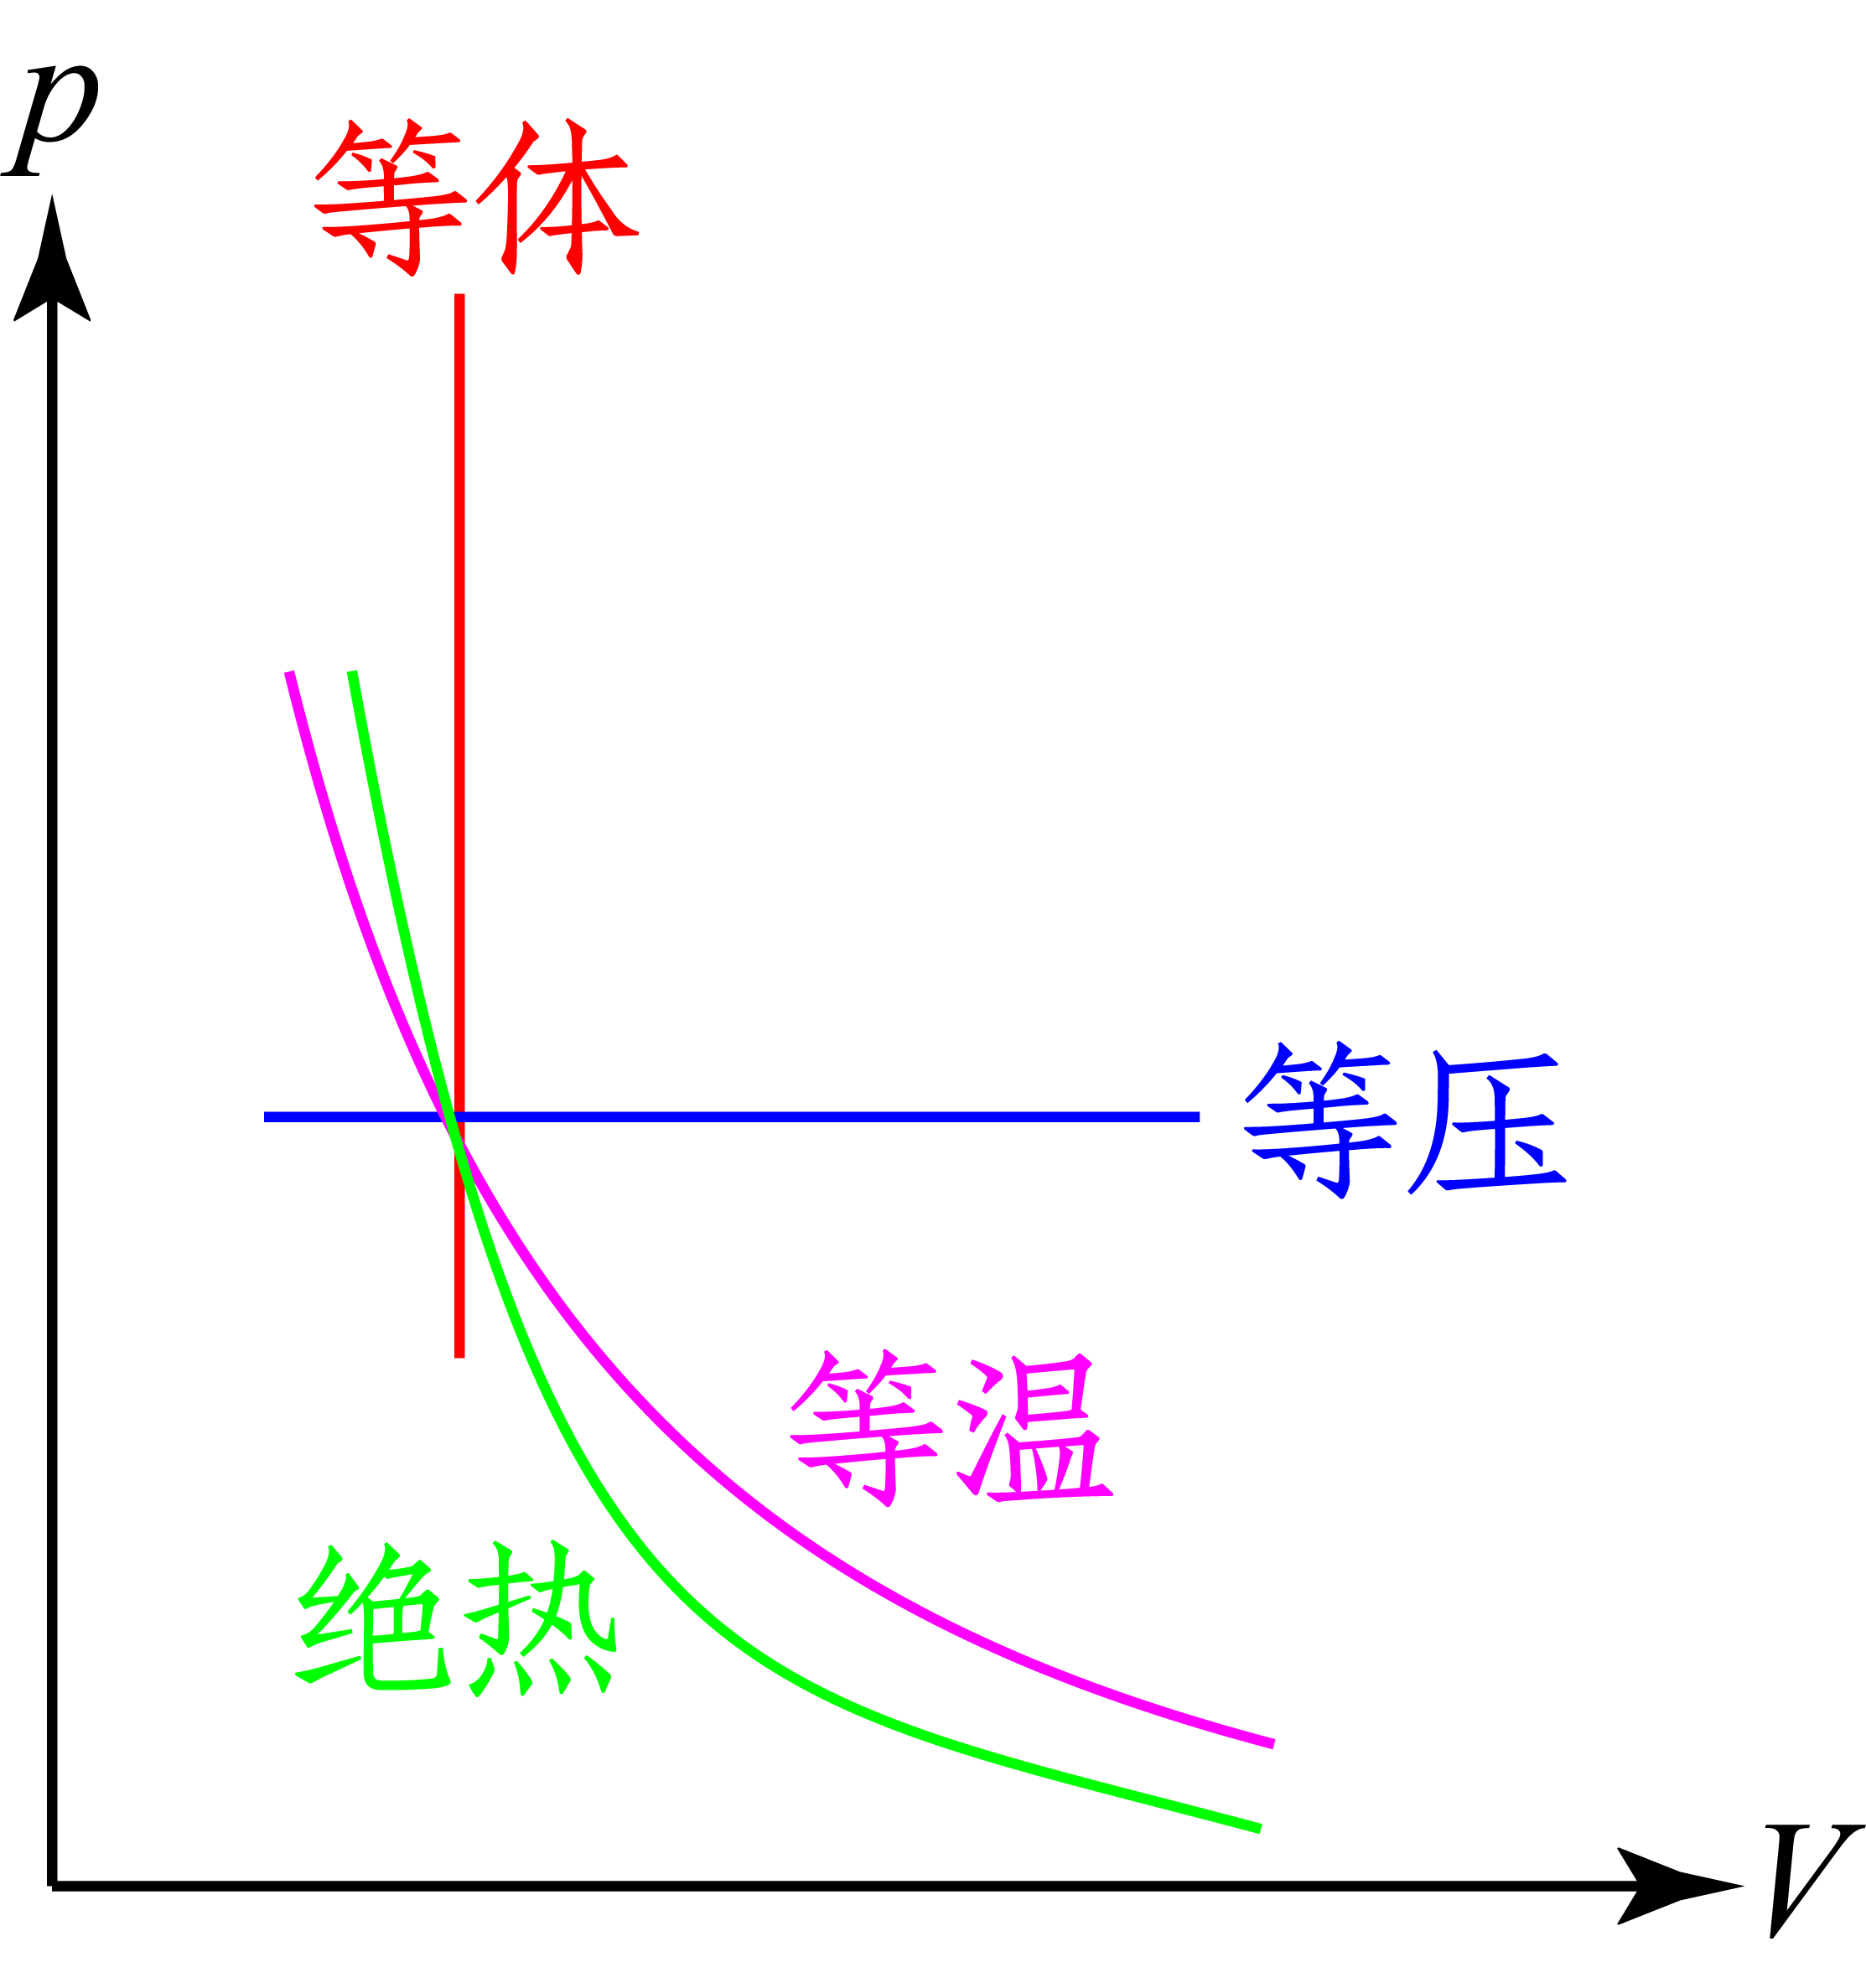
\includegraphics[width=6cm]{image/5-1-6.png}
\caption{四大准静态过程}\label{fig:1-6}
\end{wrapfigure}
所谓\emph{过程}(process)是状态的集合.\,我们考虑的范围内,\,过程的初态和末态都需要是均匀的平衡态.\,中间态如果也可以视为平衡态,\,就叫做\emph{准静态过程}(quasi-static process),\,若中间态蕴含着非平衡,\,则称为\emph{非准静态过程}(non-quasi-static process).\,下面列举常见的过程:
\subsubsection{\hei 等体过程(isochoric process)}
作为等体过程体积功为零$W=0$,\,只能以从外界吸放热$Q$(或是如图\ref{fig:1-2}所示的功变热形式.).\,系统吸热导致温度$T$升高,\,定义系统\emph{热容}(heat capacity)为:
\[C=\frac{\dbar Q}{\ud T}\]

而压强$p$将升高,\,定义\emph{压强系数}(pressure coefficient)为:
\[\beta:=\frac{1}{p}\frac{\ud p}{\ud T}\]

根据理想气体的物态方程与内能公式我们算出\footnote{热力学的角标表示这个量不变,\,而这里热容的表达式下一章学了熵的概念后可以写:\[C=T\frac{\partial S}{\partial T}\]}:
\[C_V=\left(\frac{\dbar Q}{\ud T}\right)_V=\nu C_{mV} \quad ; \quad \beta_V=\frac{1}{p}\left(\frac{\partial p}{\partial T}\right)_V=\frac{1}{T}\]

\subsubsection{\hei 准静态的等压过程(isobaric process)}
若是控制压强$p$而不是体积$V$不变,\,区别在于气体从外界吸收的热量中一部分要用来对外做功:
\[\ud U=\dbar Q-p\ud V\]

热容按同样的方法定义,\,分别称为等体热容和等压热容\footnote{中文太灵活,\,``等体''也有人说成``定体'',\,``等容'',\,``定容''.\,统一术语十分困难.}.\,而\emph{热膨胀系数}(thermal expansion coefficient)定义为:
\[\alpha:=\frac{1}{V}\frac{\ud V}{\ud T}\]

注意这实际上是\emph{体膨胀系数}(volumetric thermal expansion),\,由近似方法可知,\,近似为线膨胀系数$\alpha_L$的三倍.\,对于理想气体等压过程,\,同理可得:
\[C_p=\left(\frac{\dbar Q}{\ud T}\right)_p=\nu (C_{mV}+R)=\nu C_{mp} \quad ; \quad \alpha=\frac{1}{V}\left(\frac{\partial V}{\partial T}\right)_p=\frac{1}{T}\]

\subsubsection{\hei 准静态的等温过程(isothermal process)}
系统与恒温大热库接触,\,吸热膨胀, 压强减小;\,放热收缩,\,压强增大.\,这时$pV$为过程不变量.\,我们定义\emph{压缩系数}(compression coefficient):
\[\kappa:=-\frac{1}{V}\frac{\ud V}{\ud p}\]

注意若是在固体情形,\,以上量被称为\emph{体模量}(bulk modulus).\,对于理想气体,\,等温压缩系数为:
\[\kappa_T=-\frac{1}{V}\left(\frac{\partial V}{\partial p}\right)_T=\frac{1}{p}\]

\subsubsection{\hei 准静态的绝热过程(adiabatic process)}
绝热过程中$\dbar Q=0$,\,对于理想气体:
\[\ud U +p \ud V=0\]
\[\nu C_{mV} \ud T + \frac{\nu R T}{V}\ud V=0\]
\[C_{mV}\frac{\ud T}{T}+R\frac{\ud V}{V}=0\]

惯例上定义\emph{绝热指数}(adiabatic index)$\gamma$为:
\[\gamma:=\frac{C_{mp}}{C_{mV}}=1+\frac{R}{C_{mV}}=\frac{f+2}{f}\]

则可以由$\gamma$和$R$表示两个摩尔热容:
\[C_{mV}=\frac{1}{\gamma -1}R \quad ;\quad C_{mp}=\frac{\gamma}{\gamma -1}R\]

从而我们从绝热过程的热力学第一定律方程积分得:
\[TV^{\gamma-1}={\rm Const.}\]

也可以写为:
\[pV^\gamma={\rm Const.} \quad ; \quad \frac{p^{\gamma-1}}{T^\gamma}={\rm Const.}\]

前一式可以用于在$p-V$图\ref{fig:1-6}上确定过程曲线.\,后一式则注重关心强度量之间的变化关系而不关心广延性质.\,在绝热过程中(用角标$S$表示绝热,\,$S$其实表示熵,\,具体原因见下一章.),\,热膨胀系数,\,压强系数与压缩系数分别为:
\[\alpha_S=\frac{1}{V}\left(\frac{\partial V}{\partial T}\right)_S=-\frac{1}{\gamma -1}\frac{1}{T} \quad ;\quad \beta_S=\frac{1}{p}\left(\frac{\partial p}{\partial T}\right)_S=\frac{\gamma}{\gamma -1}\frac{1}{T}\quad ;\quad \kappa_S=-\frac{1}{V}\left(\frac{\partial V}{\partial p}\right)_S=\frac{1}{\gamma}\frac{1}{p}\]

\subsubsection{\hei 准静态的多方过程(polytropic process)}
多方过程可以由过程方程$pV^n={\rm Const.}$描述,\,多方指数$1<n<\gamma$.\,实际过程若发生缓慢,\,可以近似处理为某种形式的多段多方过程.\,多方过程的热容为:
\[C_{mn}=\left(\frac{1}{\gamma -1}-\frac{1}{n-1}\right)R\]

而其他响应函数(指上面定义的$\alpha$,\,$\beta$与$\kappa$)的形式与绝热过程算出来的类似,\,只需要把$\gamma$改为$n$.\,多方过程在特殊的参数条件下即变成以上过程:
\begin{figure}[H]
\centering
\begin{tabular}{c|c|l}
\hline
绝热指数$n$		&	摩尔热容$C_m$						&	描述			\\ \hline\hline
$n<0$ 			   		&	$\left(\dfrac{1}{\gamma -1}+\dfrac{1}{1-n}\right)R$ 		&	 吸收大量热量,\,压强体积温度同时增加			\\ \hline
$n=0$				  &	$C_{mp}$    																				&   等压过程 		    \\ \hline
$0<n<1$			&   $\left(\dfrac{1}{\gamma -1}+\dfrac{1}{1-n}\right)R$ 				&   相比吸热等温膨胀,\,温度有升高				\\ \hline
$n=1$		&	$\infty$ 																									&  	等温过程 			\\ \hline
$1<n<\gamma$		&	$ -\left(\dfrac{1}{n -1}-\dfrac{1}{\gamma -1}\right)R$ 				& 	膨胀降温时要从外界吸热 			\\ \hline
$n=\gamma$		&	$0$ 																									&	绝热过程 			\\ \hline
$n>\gamma$		&	$\left(\dfrac{1}{\gamma -1}-\dfrac{1}{n-1}\right)R$						& 	压缩气体同时给气体热量的过程	\\ \hline
$n=\infty$		&	$C_{mV}$ 																						&	等温过程			\\ \hline
\end{tabular}
\end{figure}

\subsubsection{\hei 自由膨胀过程}
\begin{wrapfigure}[15]{o}[-10pt]{6cm}
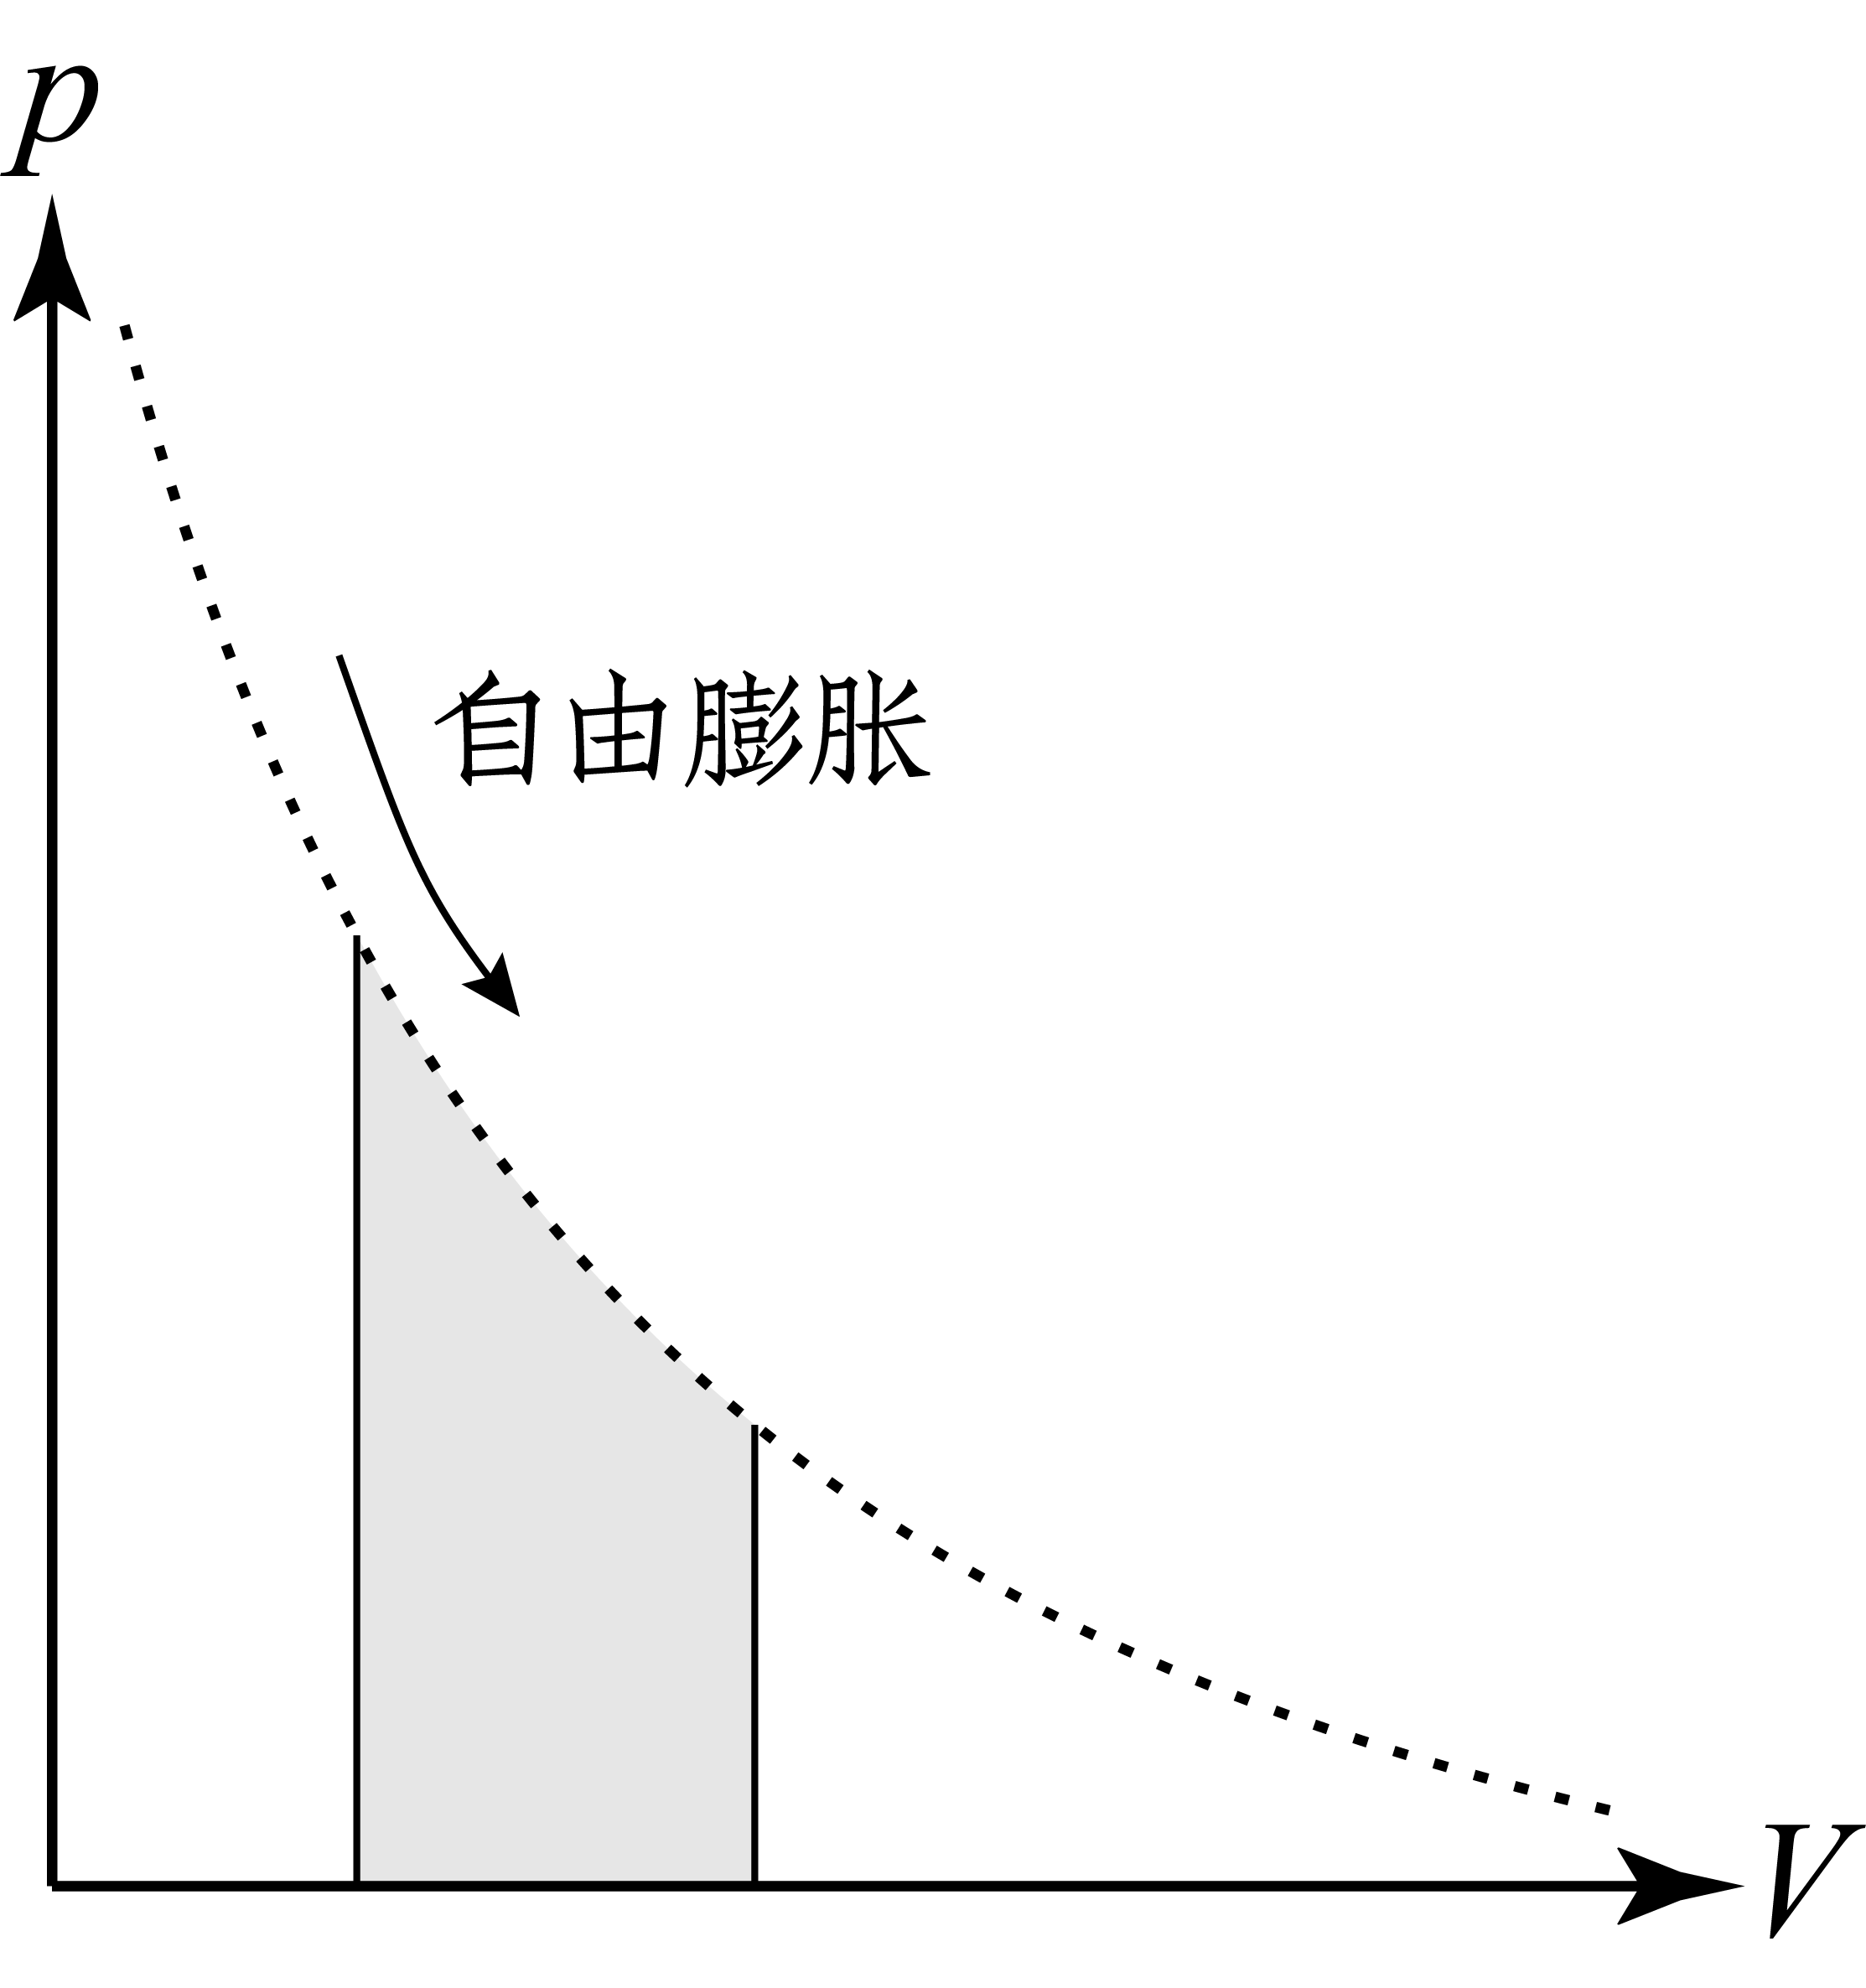
\includegraphics[width=6cm]{image/5-1-7.png}
\caption{$p-V$图上画自由膨胀}
\end{wrapfigure}
理想气体向真空的\emph{自由膨胀过程}(free expansion process)是一类典型的非准静态过程.\,在这样一个过程中,\,由于外压为零,\,外界对气体做功为零.\,而系统绝热,\,从而从外界吸热也为零.\,故由于热力学第一定律,\,内能不变.\,再根据理想气体内能直接依赖于温度的性质,\,我们发现:\,理想气体的自有膨胀是一个非准静态的等温膨胀.

从而在$p-V$图上,\,我们画一根等温线,\,它是否代表向真空的自由膨胀过程?\,我们需要画成虚线,\,线上每一个点都表示平衡态,\,而从一个点到另一个相邻的点中发生的过程则没有达到力学平衡,\,从而不能视为准静态过程.\,这一根虚线能够代表气体在自有膨胀过程中的状态,\,因为即使不均匀,\,整体的内能和可以确定出平均温度,\,整体的体积和平均温度又可以确定出平均压强.\,如果在某个时刻命自有膨胀结束,\,体系达到平衡态后其状态就落在了这根等温线上.\,只不过,\,这根线下面积此时也没有了实际意义,\,因为气体对外做功应该是零.

\vspace{2cm}

\subsubsection{\hei 向固定压强膨胀}
\begin{wrapfigure}[11]{o}[-10pt]{6cm}
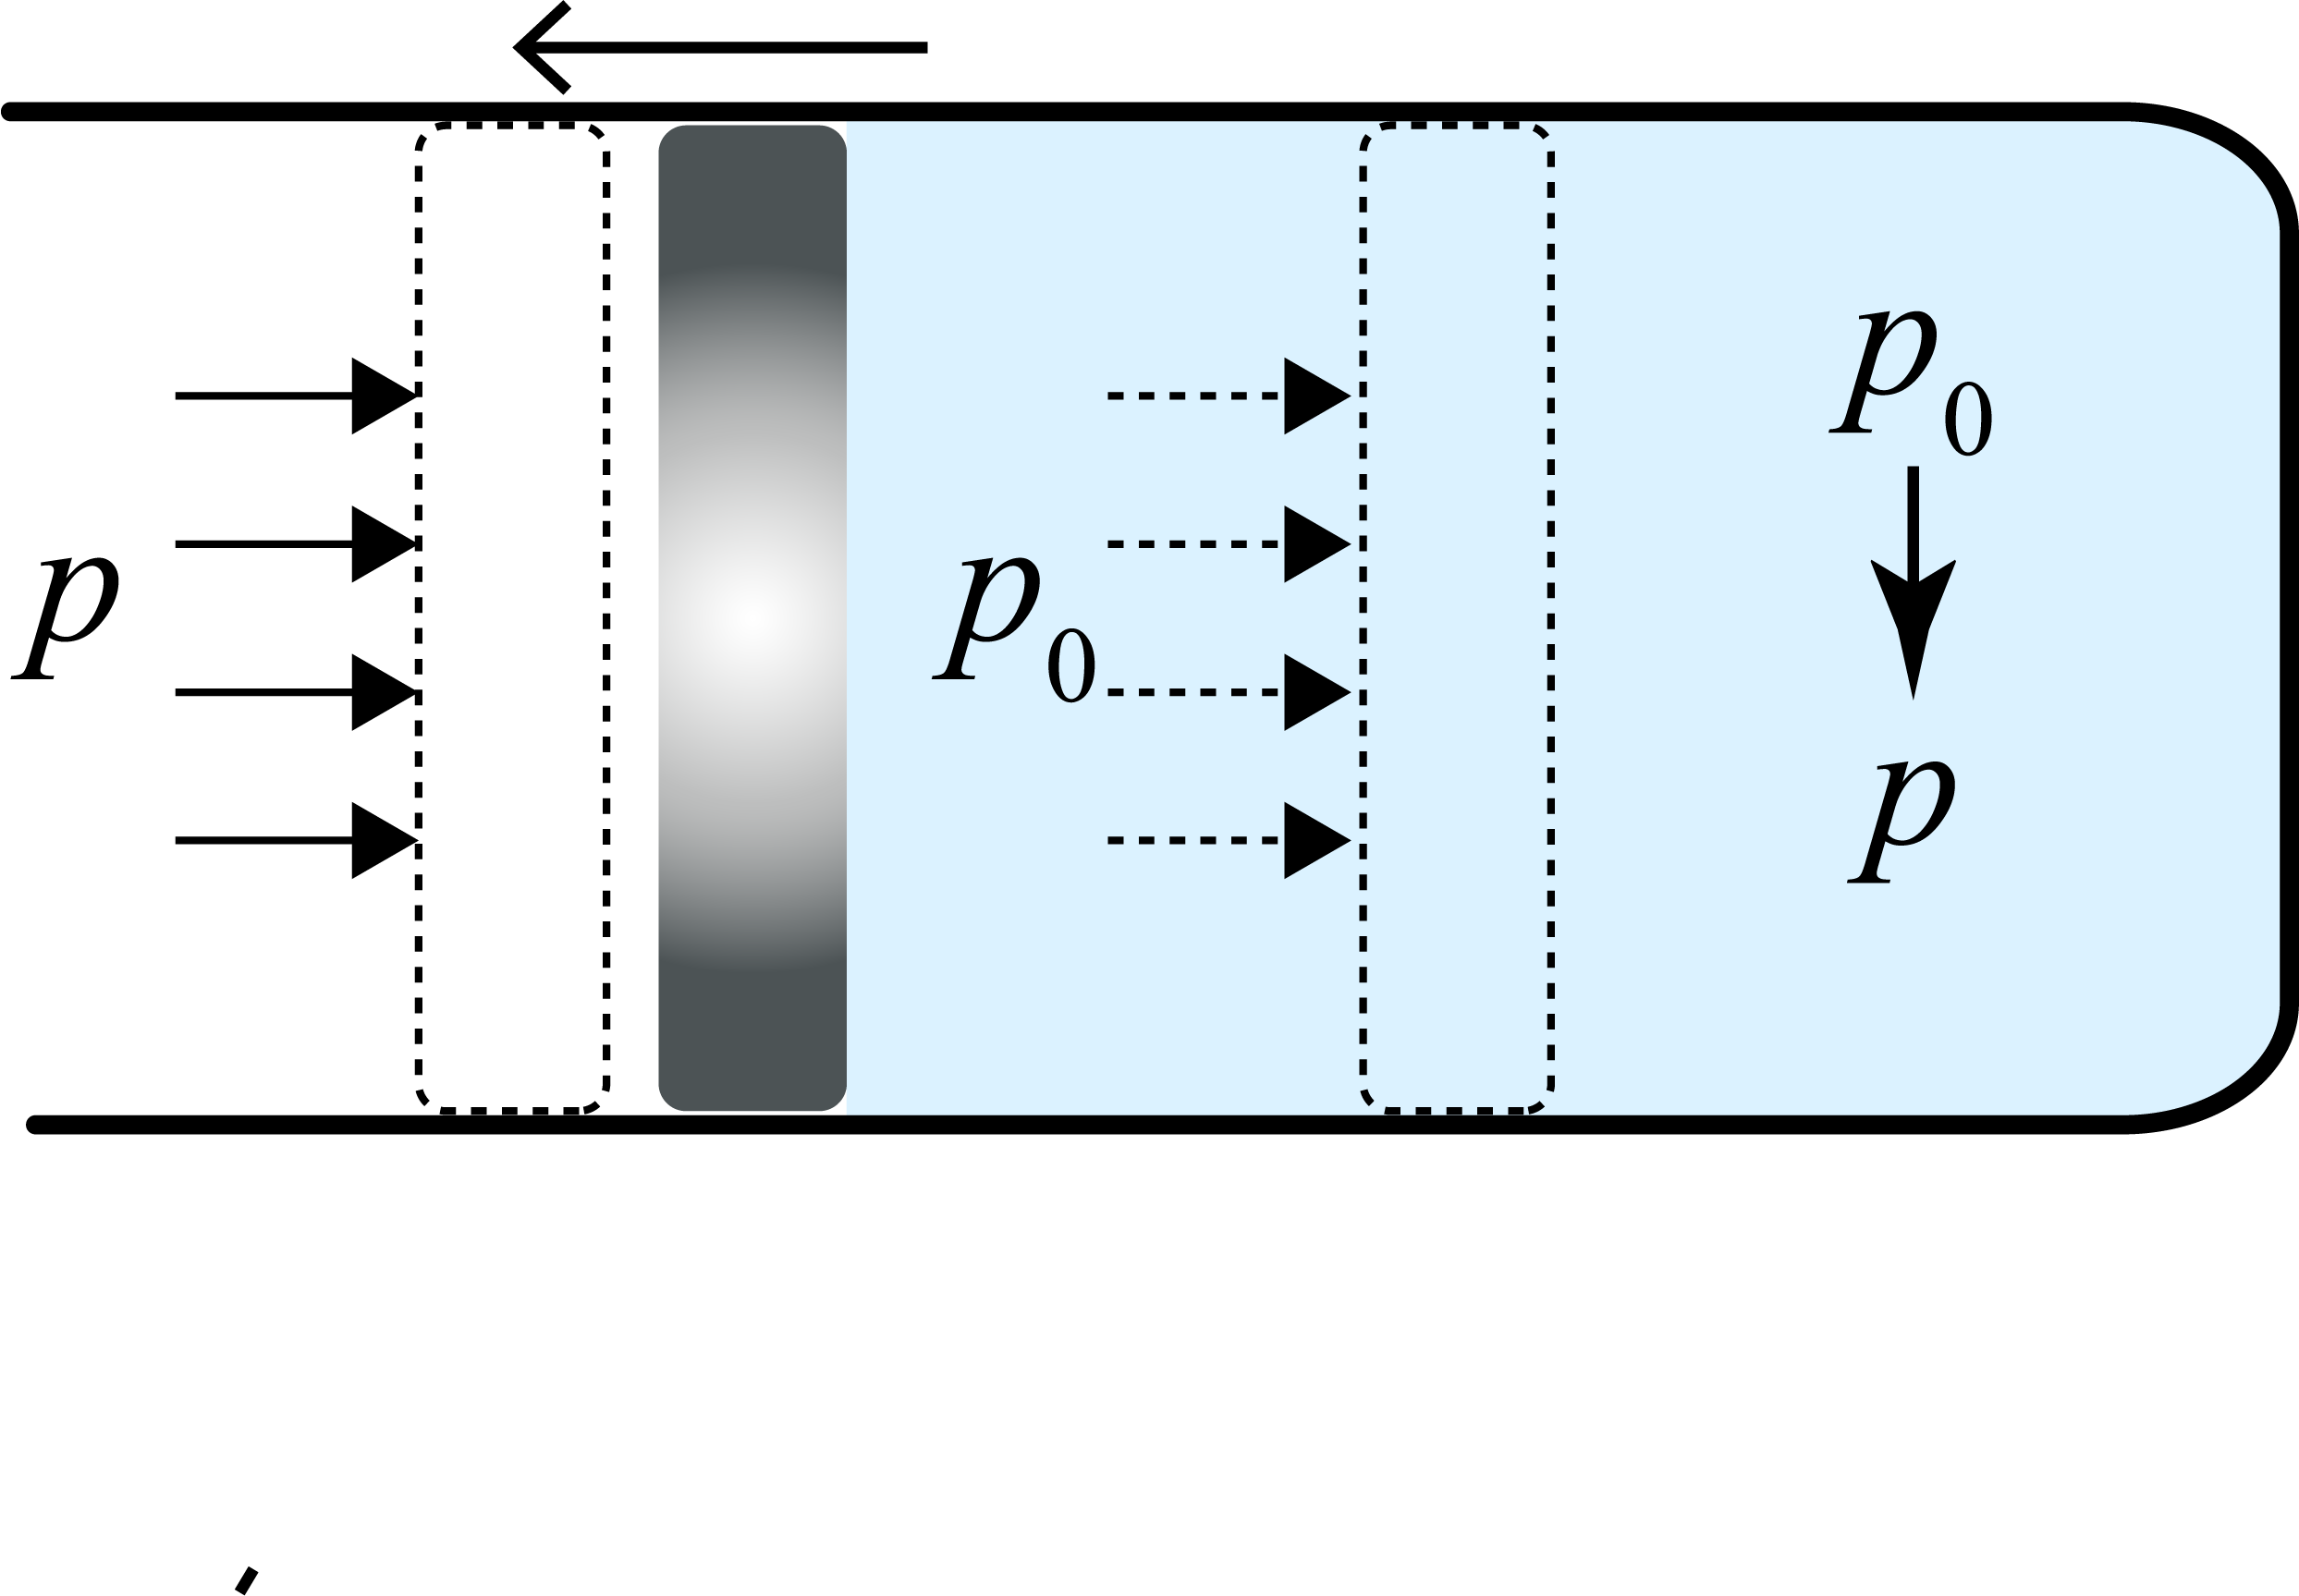
\includegraphics[width=6cm]{image/5-1-8.png}
\caption{向固定压强膨胀}
\end{wrapfigure}
考虑原平衡态压强为$p_0$的气体,\,突然命外压变小为$p$,\,气体将发生某种膨胀,\,如果膨胀稍过度,\,其压强小于外界压强$p$时,\,又会被压缩,\,这样来回振动,\,直到达到新的平衡态.\,如果这个过程系统绝热,\,则系统对外界做功应该写为:
\[W=p(V-V_0)\]

这一个模型可以这样理解:\,它保证了外界压强$p$的严格不变性.\,内部气体由于发生了急剧的体积变化,\,最靠近活塞的部分气体压强由于急剧的膨胀实际上就会等于外界气压$p$.\,这是忽略活塞质量(轻活塞)的情形.\,若是考虑活塞的质量,\,这个结论也还是成立,\,因为内外气体对活塞做功之和转化为活塞动能.\,而前后平衡态活塞实际上动能都是零.\,故内部气体对外做功可以由外界固定压强部分气体的体积功来计算.\,这就是上式.\,那么同样,\,由热力学第一定律和理想气体的性质,\,我们有:
\[\frac{V}{V_0}=1+\frac{p_0-p}{\gamma p} \quad ; \quad \frac{T}{T_0}=\frac{1}{\gamma}+(1-\frac{1}{\gamma})\frac{p}{p_0}\]

如果我们在初态压强$p_0$与末态压强$p$之间搭设很多的压强平台$p_i$,\,使得外压是缓慢地从$p_0$逐级减小到$p$,\,那么用极限的方法容易证明(请读者自己完成),\,过程恰好变为准静态的绝热过程:
\[pV^\gamma=p_0V_0^\gamma \quad ; \quad \frac{p^{\gamma-1}}{T^\gamma}=\frac{p_0^{\gamma-1}}{T_0^\gamma}\]

此时屡次的非平衡态将无限趋于平衡态,\,而非准静态过程也就无限趋于准静态过程了.

\npg{-2cm}

\subsubsection{\hei 节流过程(throttling)}
节流过程亦是对很多复杂系统过程的抽象,\,如冷凝机内部工作物质所发生的循环的定常流动.\,我们从中提取出一个模型,\,如下图,\,气体在内壁光滑的管道内做定常流动,\,通过一多孔塞后压强减小,\,气体膨胀.\,整个过程绝热.\,我们取一个固定的气团(图中红加蓝)作为研究对象.\,经过一定时间$t$后左侧与右侧体积变化分别为$V_1$与$V_2$,\,那么气体的流量被定义为:
\[Q=\frac{m_i}{t}=\frac{\rho_i V_i}{t}=\rho_i v_i A\]

由于是定常流动,\,左右两侧流量必须相等,\,这是质量守恒的要求,\,而体积流量$v_i A$可以不相等,\,因为气体可以被压缩.

下面我们考虑气体的热力学第一定律,\,由于$Q$小,\,我们忽略气体的整体动能(这一点在下一节我们将做详细讨论).\,
\begin{figure}[H]
\centering
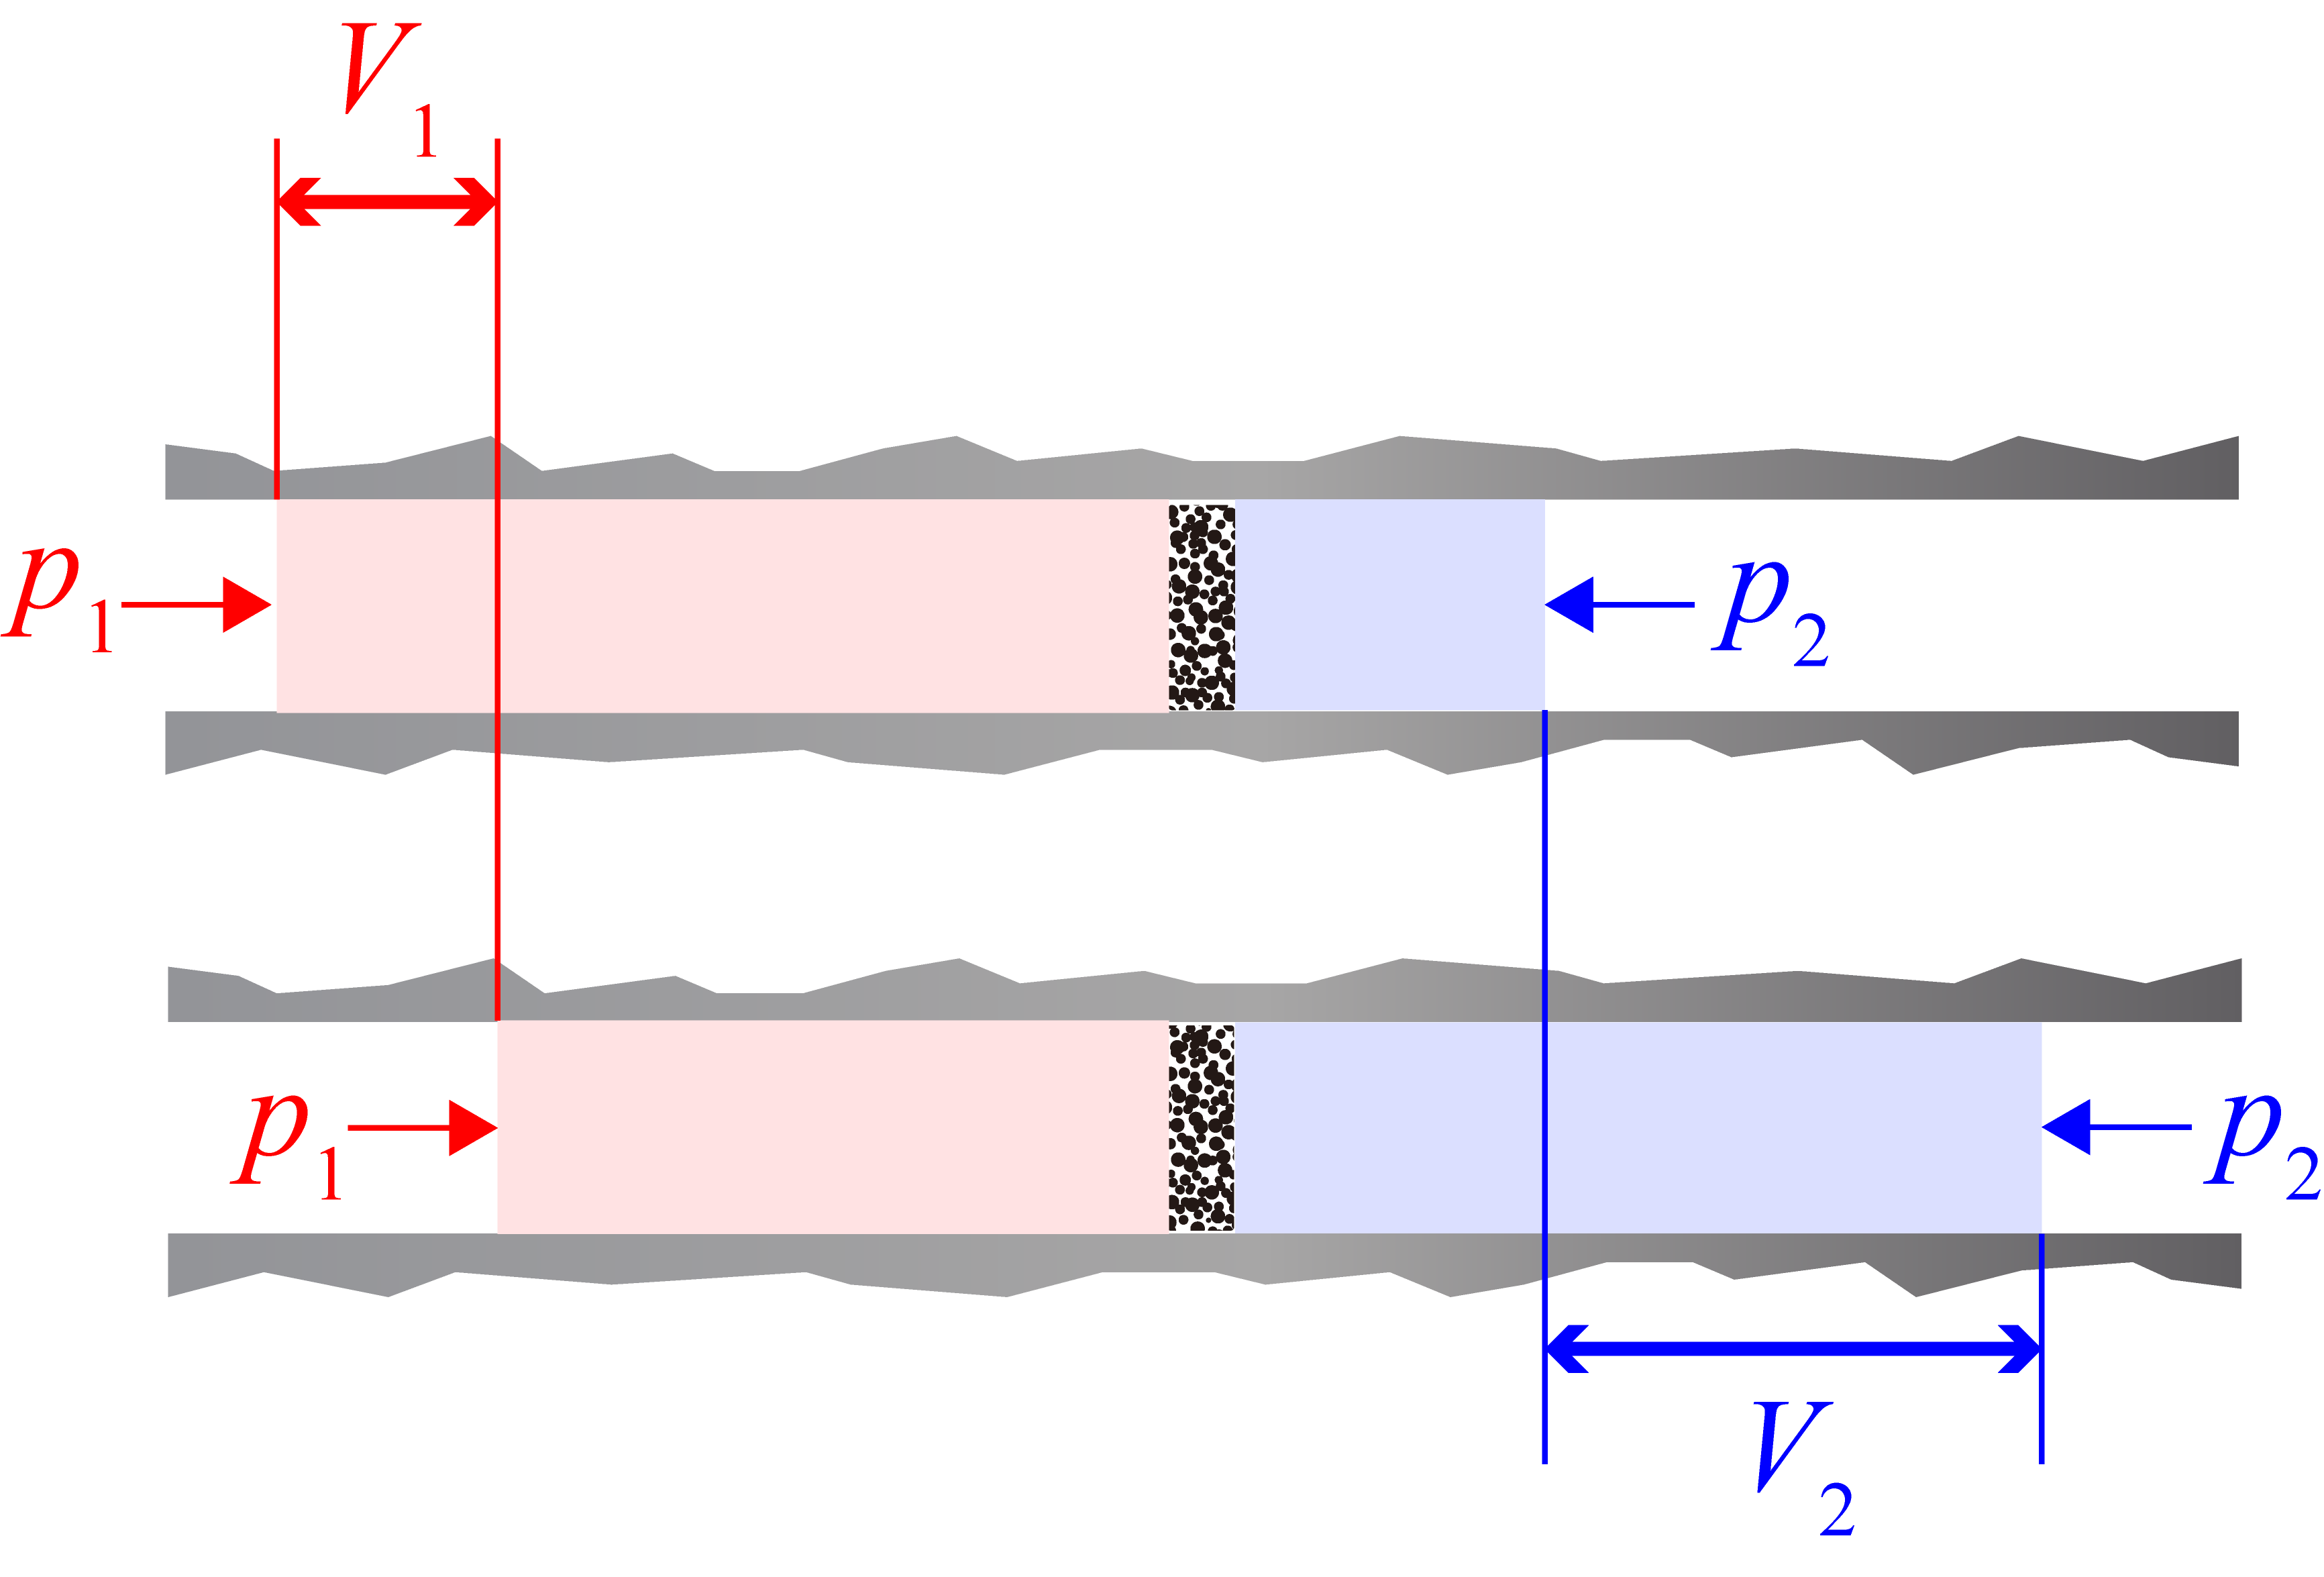
\includegraphics[width=14cm]{image/5-1-9.png}
\caption{多孔塞制节流阀}
\end{figure}

对于红+蓝的整体,\,热一定律表述为:
\[p_1V_1-p_2V_2=U_2-U_1\]

即:
\[U_1+p_1V_1=U_2+p_2V_2\quad ;\quad H_1=H_2\]

也就是说,\,节流过程前后焓不变的过程.\,若流过的气体是理想气体,\,那么
\[H=\nu C_{mV}T+pV=\nu (C_{mV}+R)T=\nu C_{mp}T\]

可见这也是一个温度不变的过程.\,但是吸热,\,做功都为零,\,它并不是一个达到平衡的准静态过程.

\npg{-2cm}

\section{开放系统的理想气体}

开放的气体系统一般有两个特点,\,一是其性质一般被描述为:\,在某处$\bs{r}$的气体性质怎样.\,而描述该气体性质的只能是各种强度量.\,如压强$p(\bs{r})$,\,温度$T(\bs{r})$等等.\,二是气体往往处于动态的物质,\,能量的交换与流动中.\,这就意味着我们分析其物理规律时必须单独取出一个\emph{气团}(parcel of air)作为研究对象.\,研究周围气体对它可能造成的微观扩散,\,黏滞,\,传热过程,\,研究周围气体对气团压力造成的体积功与加速过程.\,下面我们由简入难地分析这些问题.

\subsection{静态平衡问题\ca 重力场中的大气}
对于静态平衡的热力学体系,\,气团首先要符合的是静力学平衡条件:
\[\nabla p+\bs{f}=\bs{0}\]

其中$\bs{f}$代表体积力,\,我们考虑重力场系统,\,则为:
\[\nabla p+\rho \bs{g}=\bs{0}\]

而密度反过来又同时和压强,\,温度有关:
\[\rho=\frac{\mu p}{RT}\]

\begin{wrapfigure}[20]{o}[-10pt]{4cm}
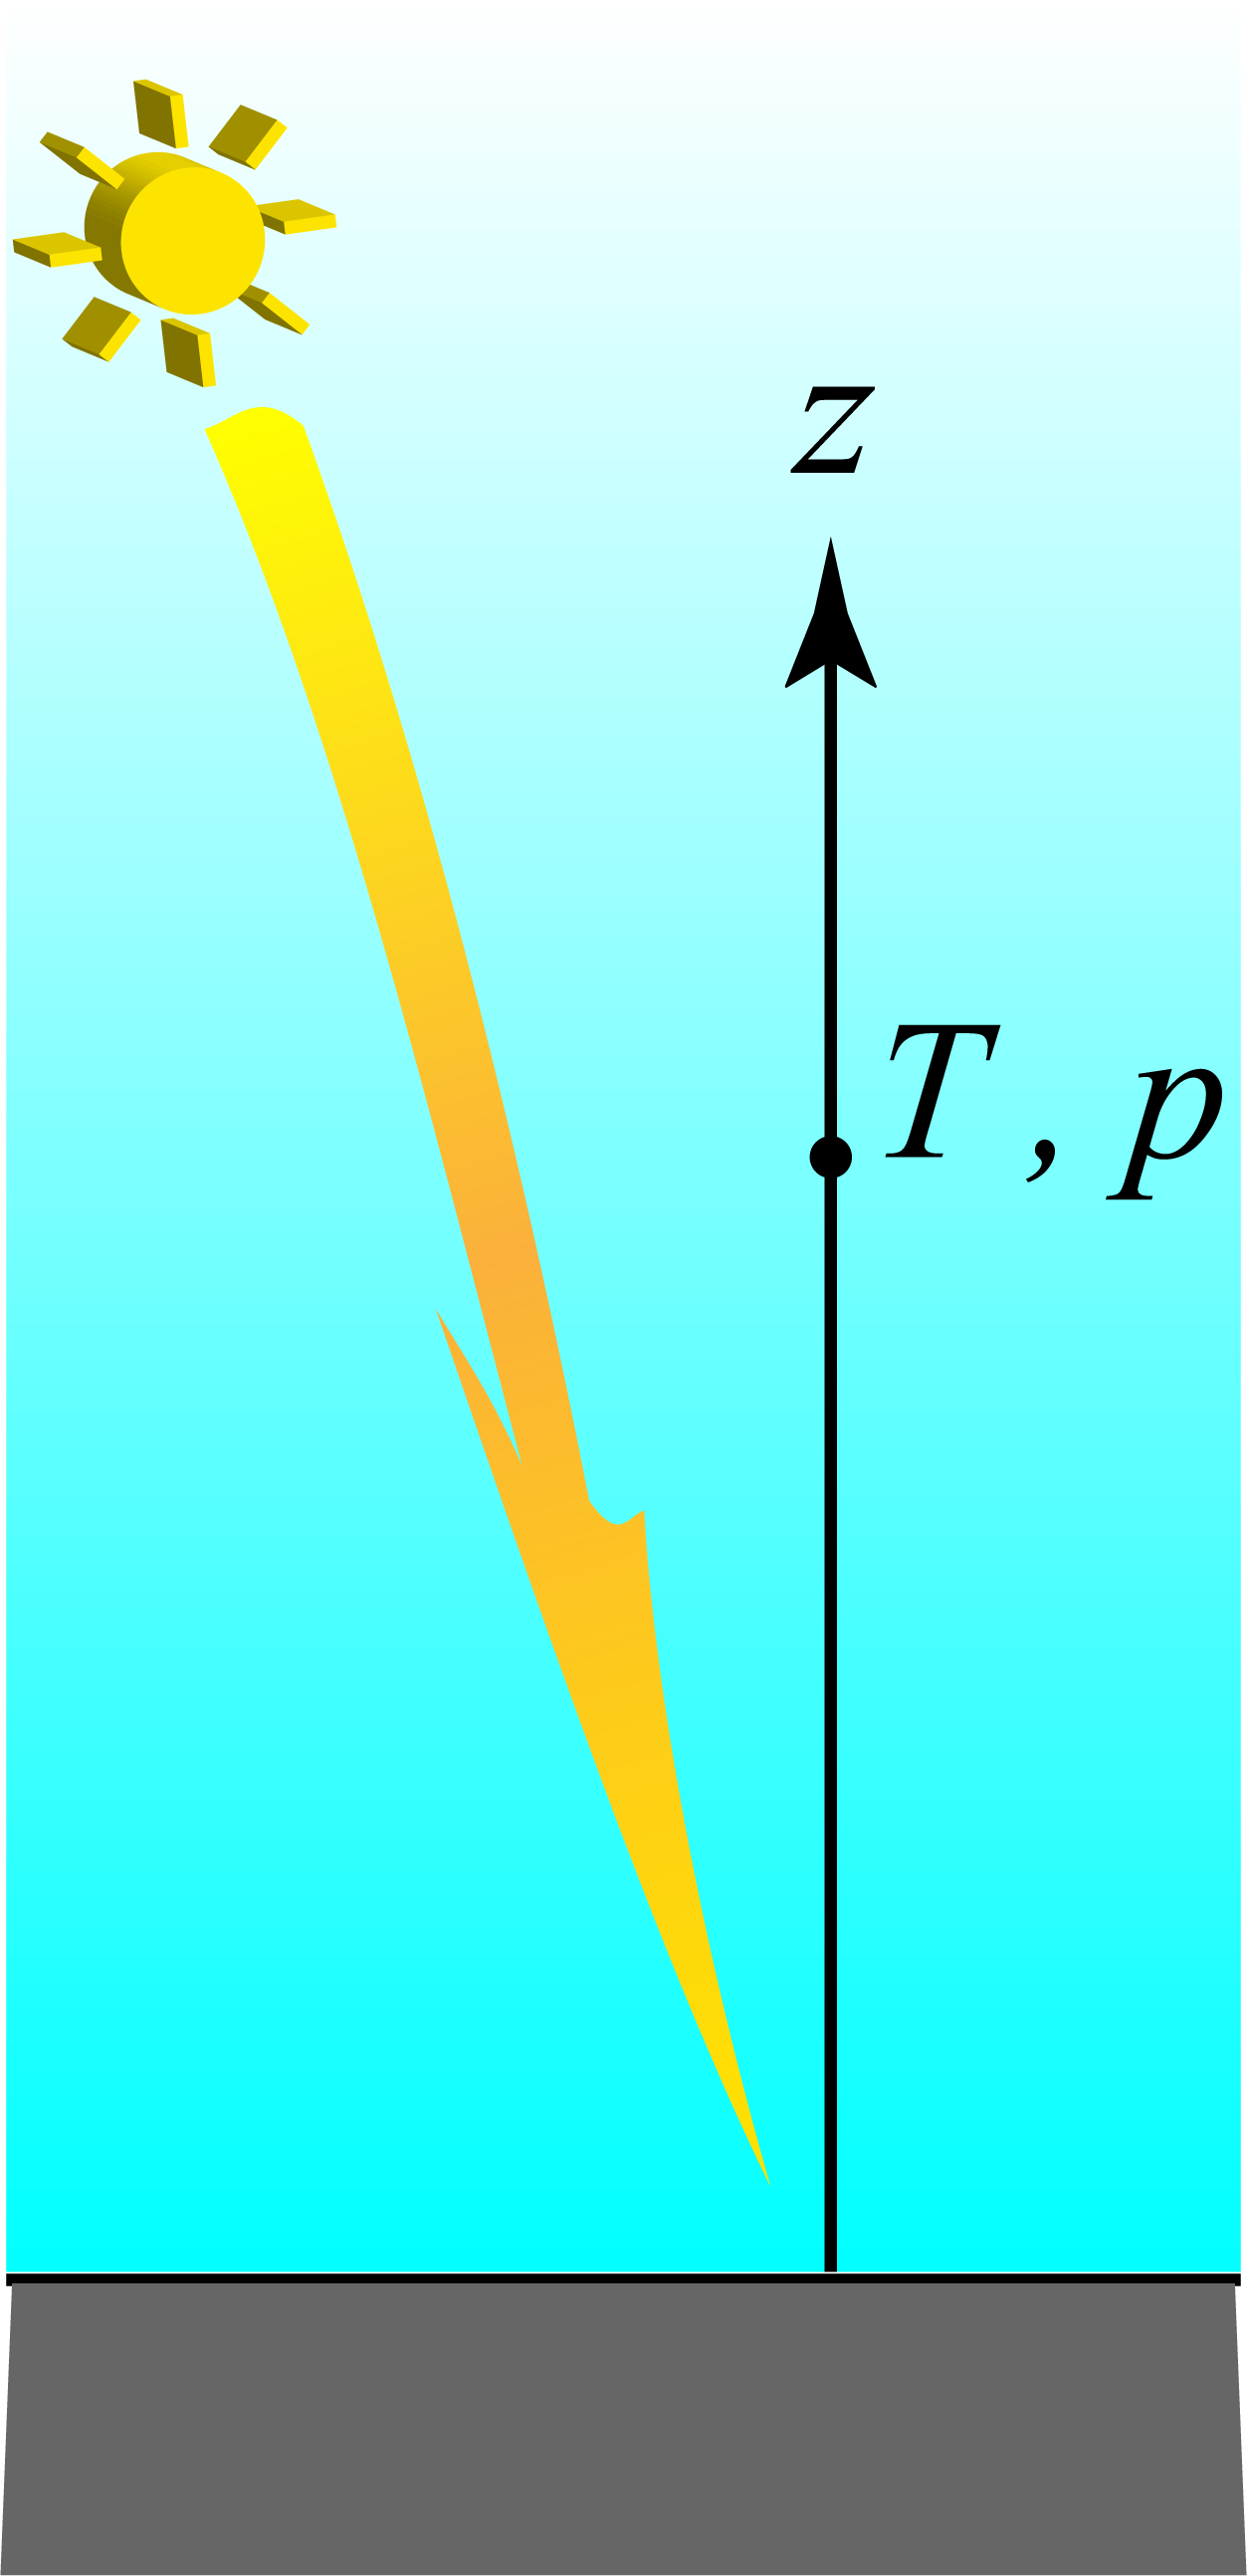
\includegraphics[width=4cm]{image/5-1-10.png}
\caption{地球大气}
\end{wrapfigure}
于是,\,压强的分布纯粹由温度分布决定,\,而温度分布则看似成为了一个纯粹的热学问题,\,而且在一定范围内粗略地研究我们可以简单地假设温度随高度均匀地变化$T(z)=T(0)-\Gamma z$.\,然而这个问题并不简单,\,大体上如果讨论限于地球表面对流层的大气,\,其基本图像可以视为由太阳照射地表,\,地表升温而加热大气导致的.\,而对于不同的气候,\,地理环境,\,时间与天气条件这个温度随高度递减的方式都十分地不相同,\,我们也还是定义\emph{环境温度递减率}(environmental lapse rate)来线性表示温度的降低:
\[\Gamma=-\frac{\ud T}{\ud z} \quad;\quad T(z)=T(0)-\Gamma z\]

了解这一点后便可计算出其压强分布:
\[p(z)=p(0)\cdot[1-\frac{\Gamma z}{T(0)}]^\frac{\mu g}{\Gamma R}=p(0)\cdot[\frac{T(z)}{T(0)}]^\frac{\mu g}{\Gamma R}\]

当环境递减率取某些不同的值时大气的性质是不同的,\,我们考虑其对流性质.\,考虑一个干的气团,\,让它在垂直方向上发生微扰,\,认为力学平衡总是很快地达到\ca 气团压强始终等于外大气压.\,但热学平衡总是来不及达到\ca 既使气团温度与外大气不相等,\,它与外界的热量交换可以忽略,\,从而可以发现,\,气团做绝热碰撞:
\[p(z)=p(0)\cdot[\frac{T'(z)}{T(0)}]^\frac{\gamma}{\gamma -1}\]

比对气团温度$T'(z)$与外大气温度$T(z)$,\,我们发现有一临界的环境温度递减率,\,我们称为\emph{干绝热递减率}(dry adiabtic lapse rate),\,它表征干燥的气团发生微扰后温度,\,密度恰好与周围大气相等的情况:
\[\Gamma_d=\frac{\gamma-1}{\gamma}\frac{\mu g}{R}=\frac{\mu g}{C_{mp}}=9.8\cdgr/\mathrm{km}\]

若$\Gamma>\Gamma_d$,\,则环境递减率过高,\,向上微扰的气团温度高于环境温度,\,所受浮力偏大,\,将偏离平衡位置,\,产生热对流,\,成云致雨.\,反之,\,$\Gamma<\Gamma_d$时浮力偏小,\,气团受到回复力而稳定在平衡位置处,\,对应着稳定无对流的大气.\,对于地球大气体系,\,有对流与无对流的情况都有时发生,\,其平均递减率就在临界绝热递减率附近.

对于临界大气为何温度随高度线性递减,\,而递减率又与定压热容有直接的关联,\,有一种较为直接的证明方法.\,其思想为虚功原理结合下面经常使用的流管分析法.\,我们让从$z=0$到$z=h$的截面积为$A$的气柱在顶部与底部的压力作用下向上发生虚位移,\,由于是临界平衡,\,故位移以后恰巧每一小块气柱$A\ud z$都与新的位置的环境大气性质全同,\,也就是与之前在这儿的那块气柱性质一样.\,整体上看,\,相当于把$z=0$处的一块质量为$\delta m$的气团位移到了$z=h$处.\,写出热力学第一定律,\,要注意其本质为能量守恒,\,这里还要包括重力势能:
\[p(0)\delta V(0)-p(h)\delta V(h)=\delta U(h)-\delta U(0)+\delta m gh\]

而由焓的定义$\delta H=\delta U +p\delta V$,\,以及理想气体的焓有公式$\delta H=\delta \nu C_{mp}T$,\,我们得出:
\[\delta \nu C_{mp}[T(0)-T(h)]=\delta \nu \mu gh\]

即:
\[T(h)=T(0)-\frac{\mu g}{C_{mp}}h\]

对于实际地球对流层大气来说,\,还需要考虑空气中水蒸气受冷造成的液化放热现象,\,其临界递减率将会取决于气体含水蒸气的多少.\,而地球下层大气还分为\emph{对流层}(troposphere)与\emph{平流层}(stratosphere),\,平流层含大量臭氧,\,太阳的紫外辐射将在传播的过程中被平流层逐渐吸收.\,所以平流层的上部具有较强的辐射和较高的平衡温度,\,而温度随高度递增,\,提供了一个稳定的大气环境,\,极难发生对流.





\subsection{能量守恒\ca 伯努利方程}
我们把流体力学里讨论的\emph{伯努利方程}(Bernoulli Equation)推广到热力学中.\,它适用条件为\emph{定常流动}(steady flow)中的同一条\emph{流线}(streamline)上.\,它也是推广的热力学第一定律,\,它代表能量的守恒.

\begin{wrapfigure}[10]{o}[-10pt]{6cm}
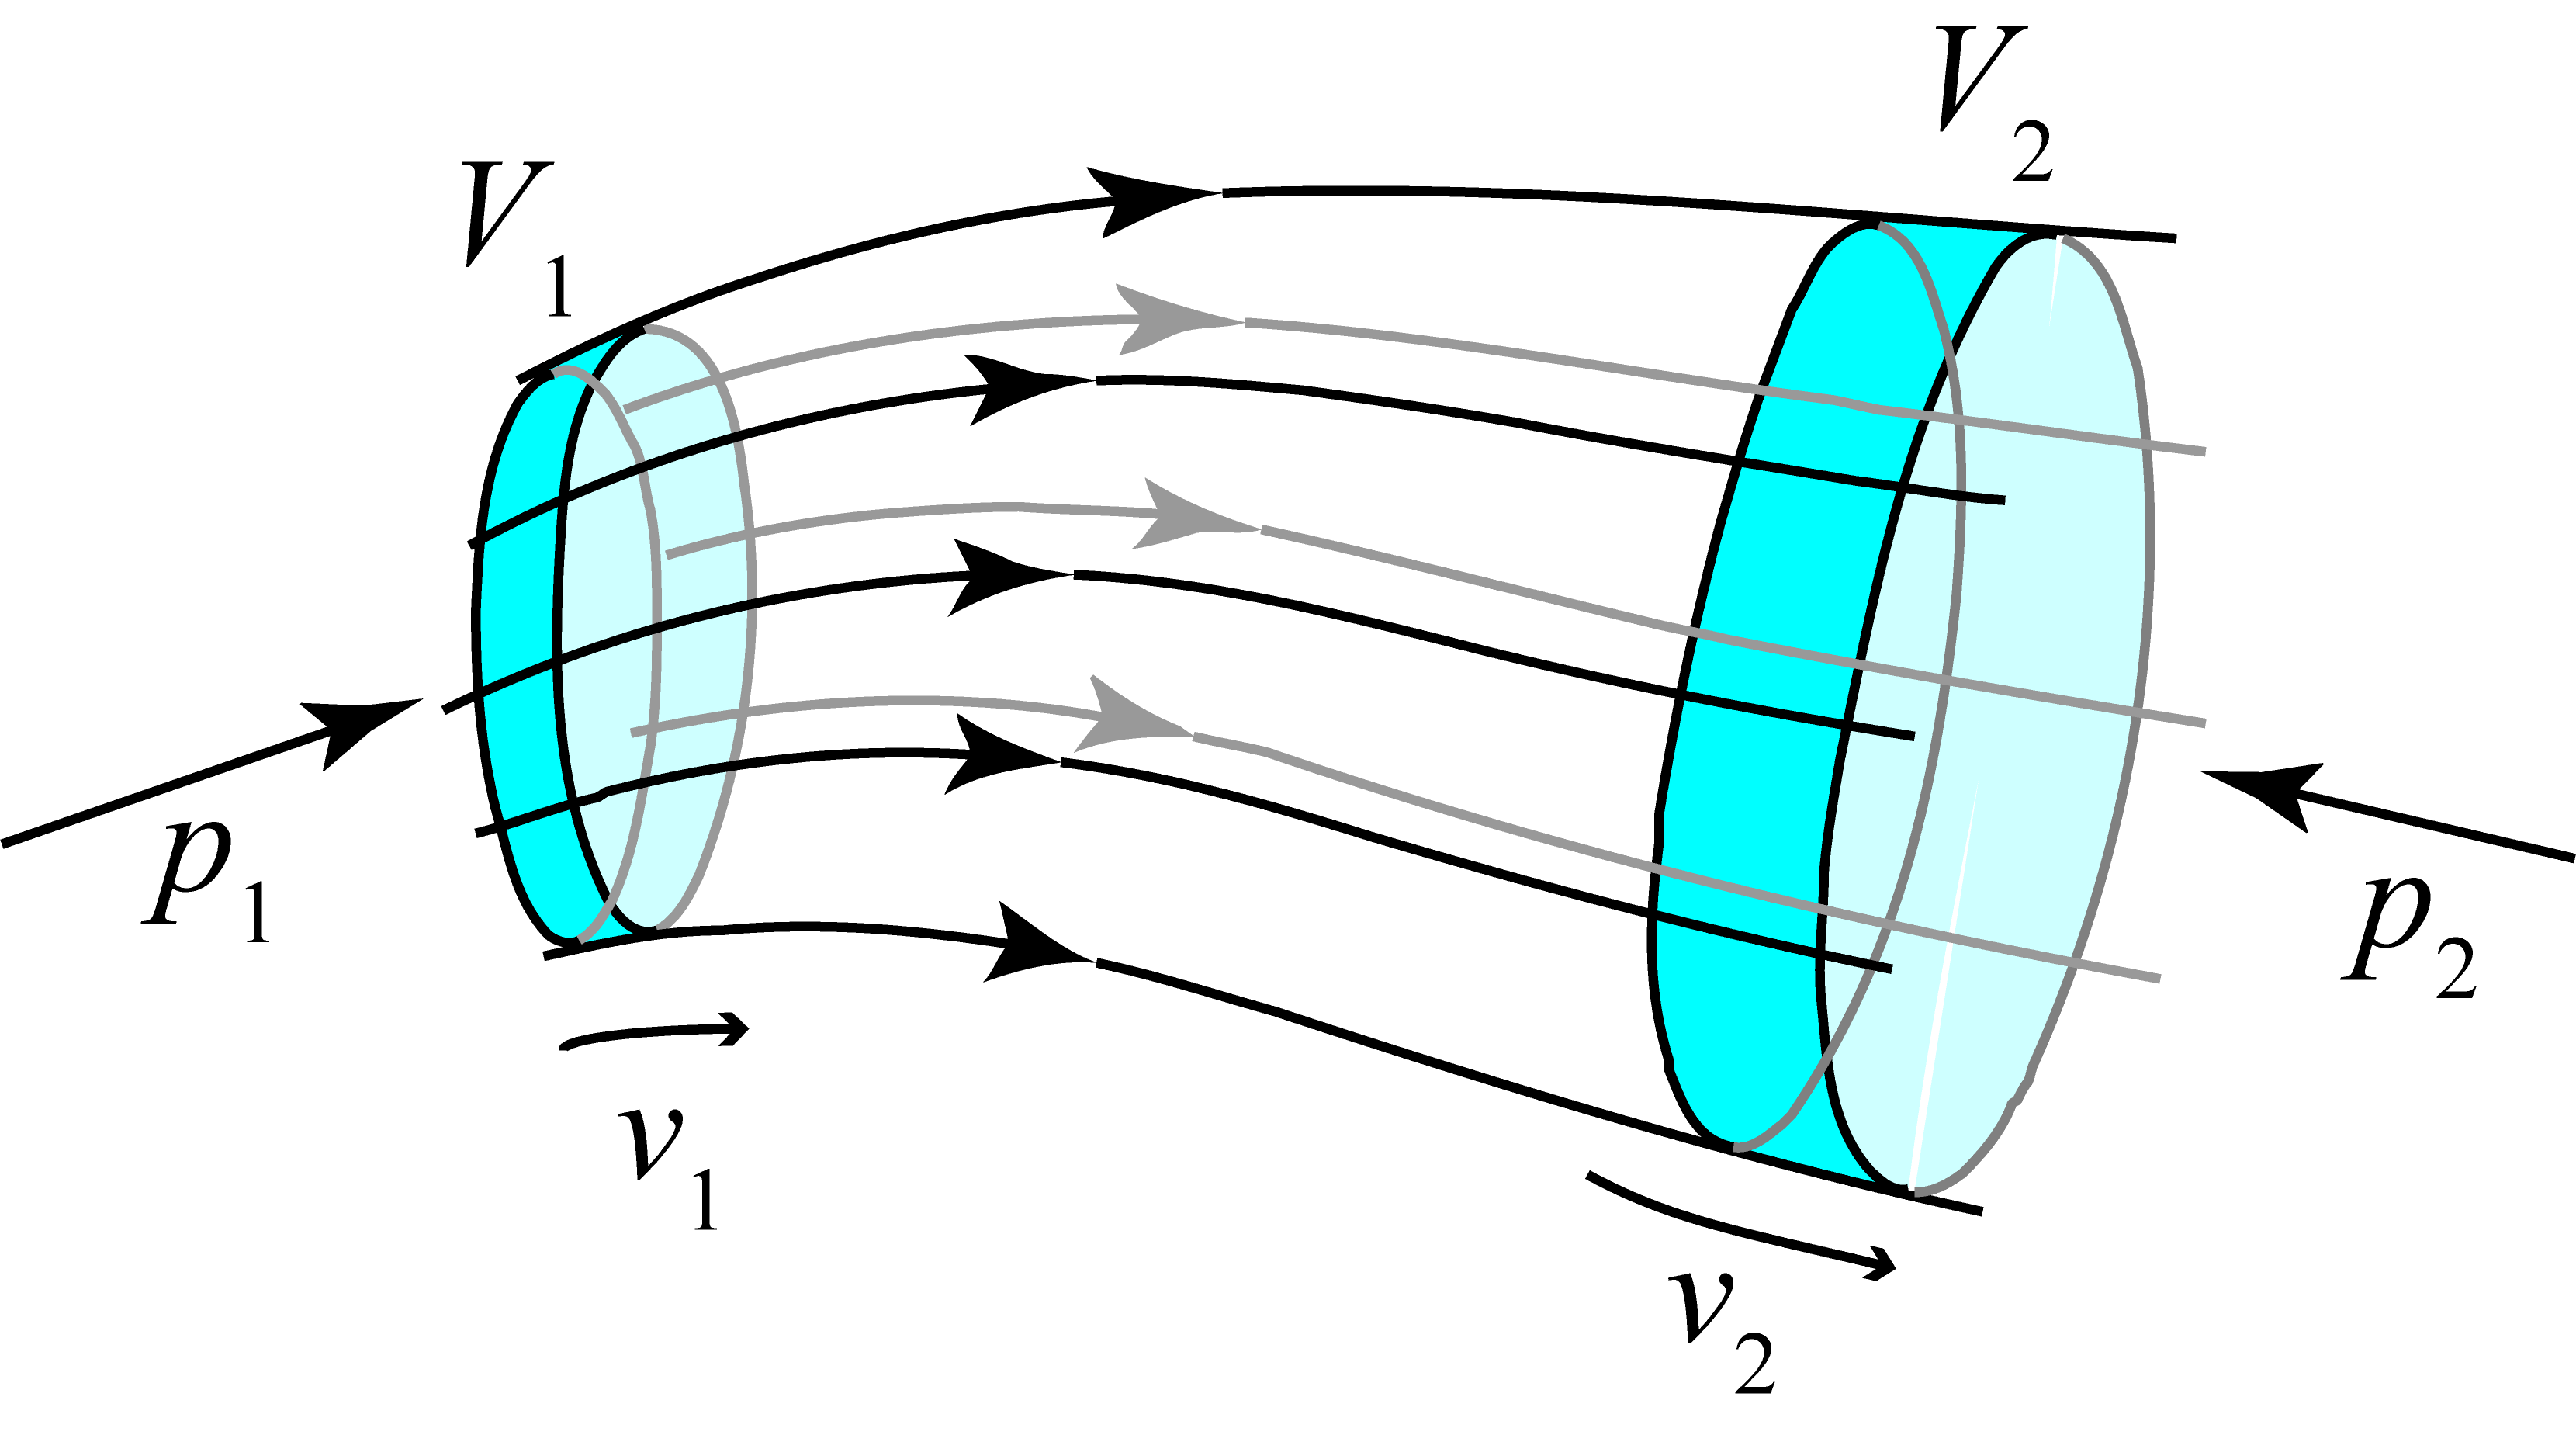
\includegraphics[width=6cm]{image/5-1-11.png}
\caption{气体沿一条流管流动}
\end{wrapfigure}
不可压缩流体的伯努利方程的图像其实很清晰,\,我们若不考虑流体势能的变化,\,那么伯努利原理实际是在说,\,两侧的压强差导致了流体的加速:
\[p_1-p_2=\frac{1}{2}\rho v_2^2-\frac{1}{2}\rho v_1^2\]

从而沿流线,\,以下量守恒:
\[p+\frac{1}{2}\rho v^2=\mathrm{const.}\]

但若考虑可以压缩的气体,\,以及考虑保守外力的做功,\,是否有以上守恒量呢?\,我们假设保守外力为质量力:\,单位质量的流体的势能为$\Phi$,\,那么对于一定时间间隔$t$下的流管发生的流动$m=Qt$,\,有以下能量守恒:
\[p_1V_1-p_2V_2=(U_2+\frac{1}{2}mv_2^2+m\Phi_2)-(U_1+\frac{1}{2}mv_1^2+m\Phi_1)\]

两边同时除以质量,\,得守恒律:
\[u+\frac{p}{\rho}+\frac{v^2}{2}+\Phi=\mathrm{const.}\]

其中$u+p/\rho=u+pv=h$即为比焓,\,而$u$为比内能,\,$v$为比体积,\,``比''表示单位质量的某物理量,\,它是一种强度量.\,从而以上量我们还可以写为:
\[h+\frac{v^2}{2}+\Phi=\mathrm{const.}\]

我们还定义所谓的\emph{阻滞焓}(stagnation enthalpy)的概念.\,它表示让运动的气体发生某种虚构的定常流动绝热地停止下来后气体应该有的焓.\,那么比阻滞焓为:
\[h'=h+\frac{v^2}{2}\]

最后这一广义的伯努利方程,\,就被我们写为一个广义的两项的能量守恒形式:
\[h'+\Phi=\mathrm{const.}\]

那么对于理想气体,\,我们还可以定义阻滞温度:
\[T'=T+\frac{\mu v^2}{2C_{mp}} \quad ; \quad h'=\frac{1}{\mu}C_{mp}T'\]

而对于普通不可压缩流体,\,我们一般不关心其热学性质,\,故焓可以扣除内能项$h=p/\rho +v^2/2$,\,而$\rho$为常数.\,这样我们又可以定义阻滞压强:
\[p'=p+\frac{1}{2}\rho v^2\quad;\quad h'=\frac{p'}{\rho}\]




\subsection{动量守恒\ca 欧拉方程}
让我们考虑管道内的理想气体流动,\,管道的截面积在不断减小的情况$A=A(x)$.\,可以想见,\,这会导致流速的增加,\,进一步导致压强的减小,\,对应方程为\emph{连续性方程}(continuity equation)与伯努利方程,\,分别对应质量与能量守恒:
\[\rho vA=\mathrm{const.}\]
\[\frac{1}{\mu}C_{mp}T+\frac{v^2}{2}=\mathrm{const.}\]

以上方程还应联系物态方程理解:
\[\rho=\frac{\mu p}{RT}\]

\begin{figure}[H]
\centering
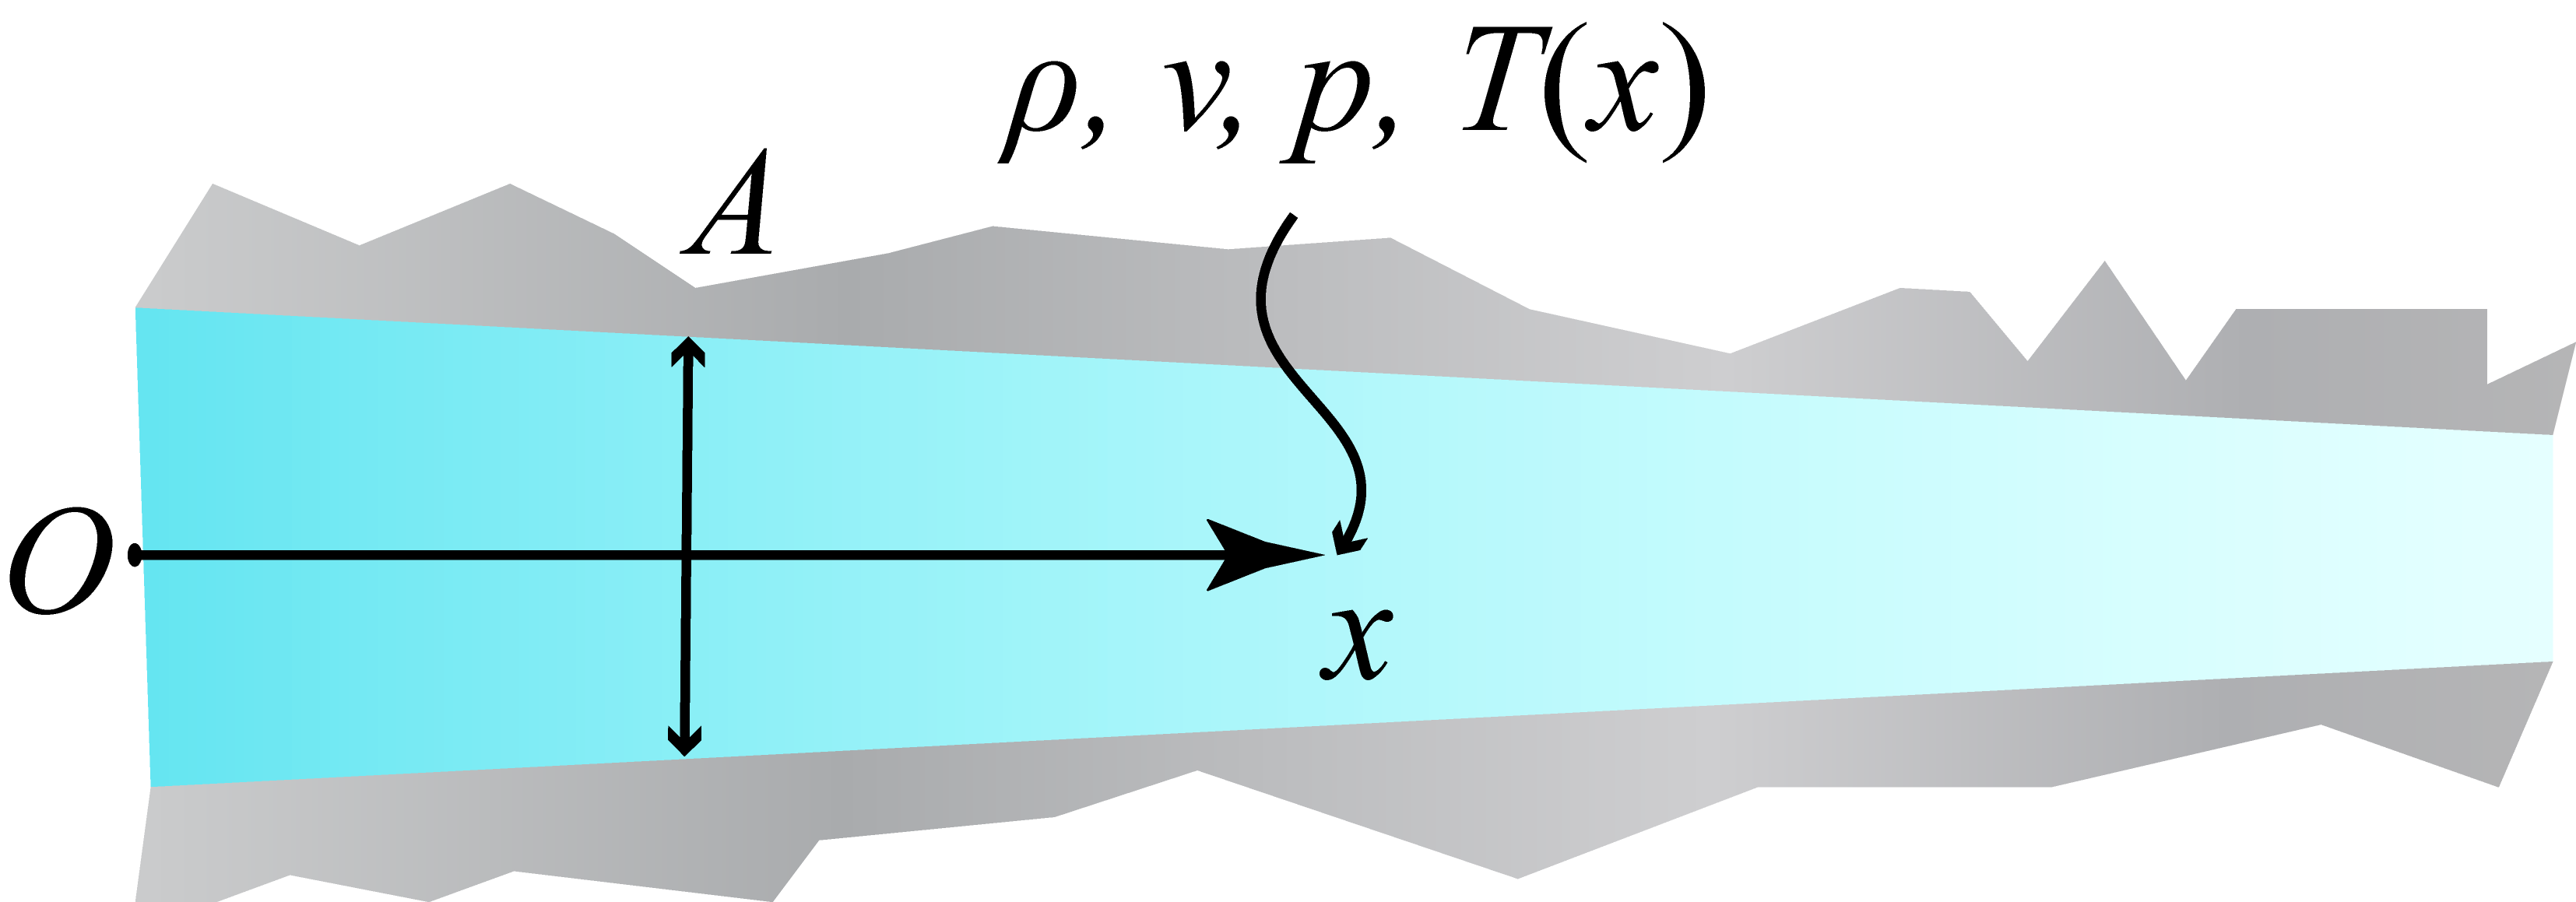
\includegraphics[width=12cm]{image/5-1-12.png}
\caption{截面积减小的管道内的气流}
\end{figure}



注意到我们把$A$的变化当做已知量以后,\,却仍设了待求解的四个物理量$v(x),\,p(x),\,T(x),\,\rho(x)$,\,但目前却只有三个方程.\,那么我们漏了怎样一个方程呢?\,这个方程就是流体的\emph{欧拉方程}(Euler equation),\,它是一个纯粹的动力学方程,\,不包含任何热效应.\,一般写作:
\[\frac{\mathrm{D} \bs{v}}{\mathrm{D} t}=-\frac{\nabla p}{\rho}-\nabla \Phi\]

其中$\mathrm{D}$代表\emph{随体导数}(material derivative):
\[\frac{\mathrm{D}}{\mathrm{D} t}=\frac{\ud}{\ud t}+\bs{v}\cdot \nabla\]

上式代表了压强梯度力与保守外力对流体的加速效应,\,在上述情形中没有外力所以等式右边只有一项.\,实际上,\,它代表了整个体系动量守恒.\,而对于上述情形,\,气体做定常流动,\,上式写为:
\[v\frac{\ud v}{\ud x}=-\frac{1}{\rho}\frac{\ud p}{\ud x}\]

这一个式子也可以由上一节的类似方法\ca 取一定长度的气团来导出.\,但切不可忽略管壁对气体在过程中作用的冲量:
\[p_1A_1\bs{e}_x \cdot t-p_2A_2\bs{e}_x \cdot t+\int -p\ud \bs{A} \cdot t=m\bs{v}_2-m\bs{v}_1\]

左边恰巧是在整个表面的压强的面积分,\,可以由高斯定理化为体积内的体积分:
\[\int_{x_1}^{x_2}-\frac{\ud p}{\ud x}\cdot A\ud x=Q(v_2-v_1)\]

又考虑到以上积分式无法直接积出结果,\,故对积分上限求导,\,再考虑到$Q=\rho vA$,\,化简后即得欧拉方程:
\[\frac{\ud p}{\ud x}=-\rho v\frac{\ud v}{\ud x}\]

对于管道截面积相对于长度变化缓慢的情况\footnote{即,\,在所关心的范围内截面积的相对变化很小:\[\frac{\Delta A}{A}\ll 1\]},\,联立以上四个方程,\,解得:
\[\frac{\ud v}{v}=-\frac{\ud A}{A}(1-\frac{\mu v^2}{\gamma RT})^{-1}\]
\[\ud p=\rho v^2\cdot\frac{\ud A}{A}(1-\frac{\mu v^2}{\gamma RT})^{-1}\]
\[\ud T=\frac{\mu v^2}{C_{mp}}\cdot\frac{\ud A}{A}(1-\frac{\mu v^2}{\gamma RT})^{-1}\]

可见,\,随着截面积$A$的减小,\,流速加快,\,压强和温度都要减小,\,利用这个效应可以制作纯粹依靠风力制冷的``土空调''.\,注意到以上结论还依赖于一个条件:
\[\frac{\mu v^2}{\gamma RT}<1\]

这意味着分子代表的气团集体运动能量要远小于分母代表的微观热运动能量,\,这在一般情况下是很容易满足的,\,因为$v\sim 10 \mathrm{m/s}$而热运动平均速率$\bar{v}\simeq 500 \mathrm{m/s}$,\,若对于高速运动的气体,\,其发生的过程中气团速度的改变与热运动平均速度可以比拟,\,实际上把气团处理为平衡的理想气体也是不妥当的.
%!TEX root = ../physical-olympics-2.tex
\chapter{热力学第二定律}


热力学第一定律固然强大,\,它根本上杜绝了所谓的\emph{第一类永动机}(perpetual motion machine of the first kind)的可能性,\,也排除了一大类不现实的热力学过程的发生.\,然而由这样一个只关心整体性质,\,不深入到微观本质的热力学规律又能告诉我们多少呢?\,\emph{炼金术}(alchemy)不违背热力学第一定律,\,它企图实现物质与物质之间的随意转化,\,\emph{第二类永动机}(perpetual motion machine of the second kind)亦不违背热力学第一定律,\,它基于能量守恒,\,主张同一份能源的无限再生利用.\,对于前者,\,微观机理彻底地否定了它,\,不同的原子有不同的构成,\,原子核的结构十分稳定,\,至今无法自由操控.\,而对于后者,\,统计规律也彻底地进行了否定,\,它告诉我们,\,一个体系的过程总是有确定的方向性,\,在一定条件下,\,过程被我们分类为\emph{自发过程}(spontaneous process)与\emph{不自发过程}(non-spontaneous process),\,具有特定方向性的过程一旦发生,\,其时间反演的过程就将不现实.\,但十分神奇的一点是,\,不同体系的不可逆特性居然是紧密相关的,\,若将一个过程的不可逆性与另一个不可逆过程的不可逆性建立联系,\,我们就能从中同时发现统一的热力学温标与态函数熵这两个概念,\,从而量化过程的不可逆性,\,这一套宏观的规律称为热力学第二定律.\,它道出了热力学过程的方向性,\,本质是微观统计规律,\,限制了另一大类不现实的热力学过程的发生.


\section{循环过程}
在历史上,\,热力学基本规律的确立与发展和热机的使用与改进是紧密相关的.\,直到今天卡诺循环的引入仍然不失为介绍热力学第二定律理论体系的强有力工具.\,本节将介绍热机,\,热泵的基本模型与著名的卡诺循环.\,为之后引入热力学第二定律相关概念打下基础.

\subsection{热机与热泵}
\begin{wrapfigure}[13]{o}[-10pt]{7cm}
\centering
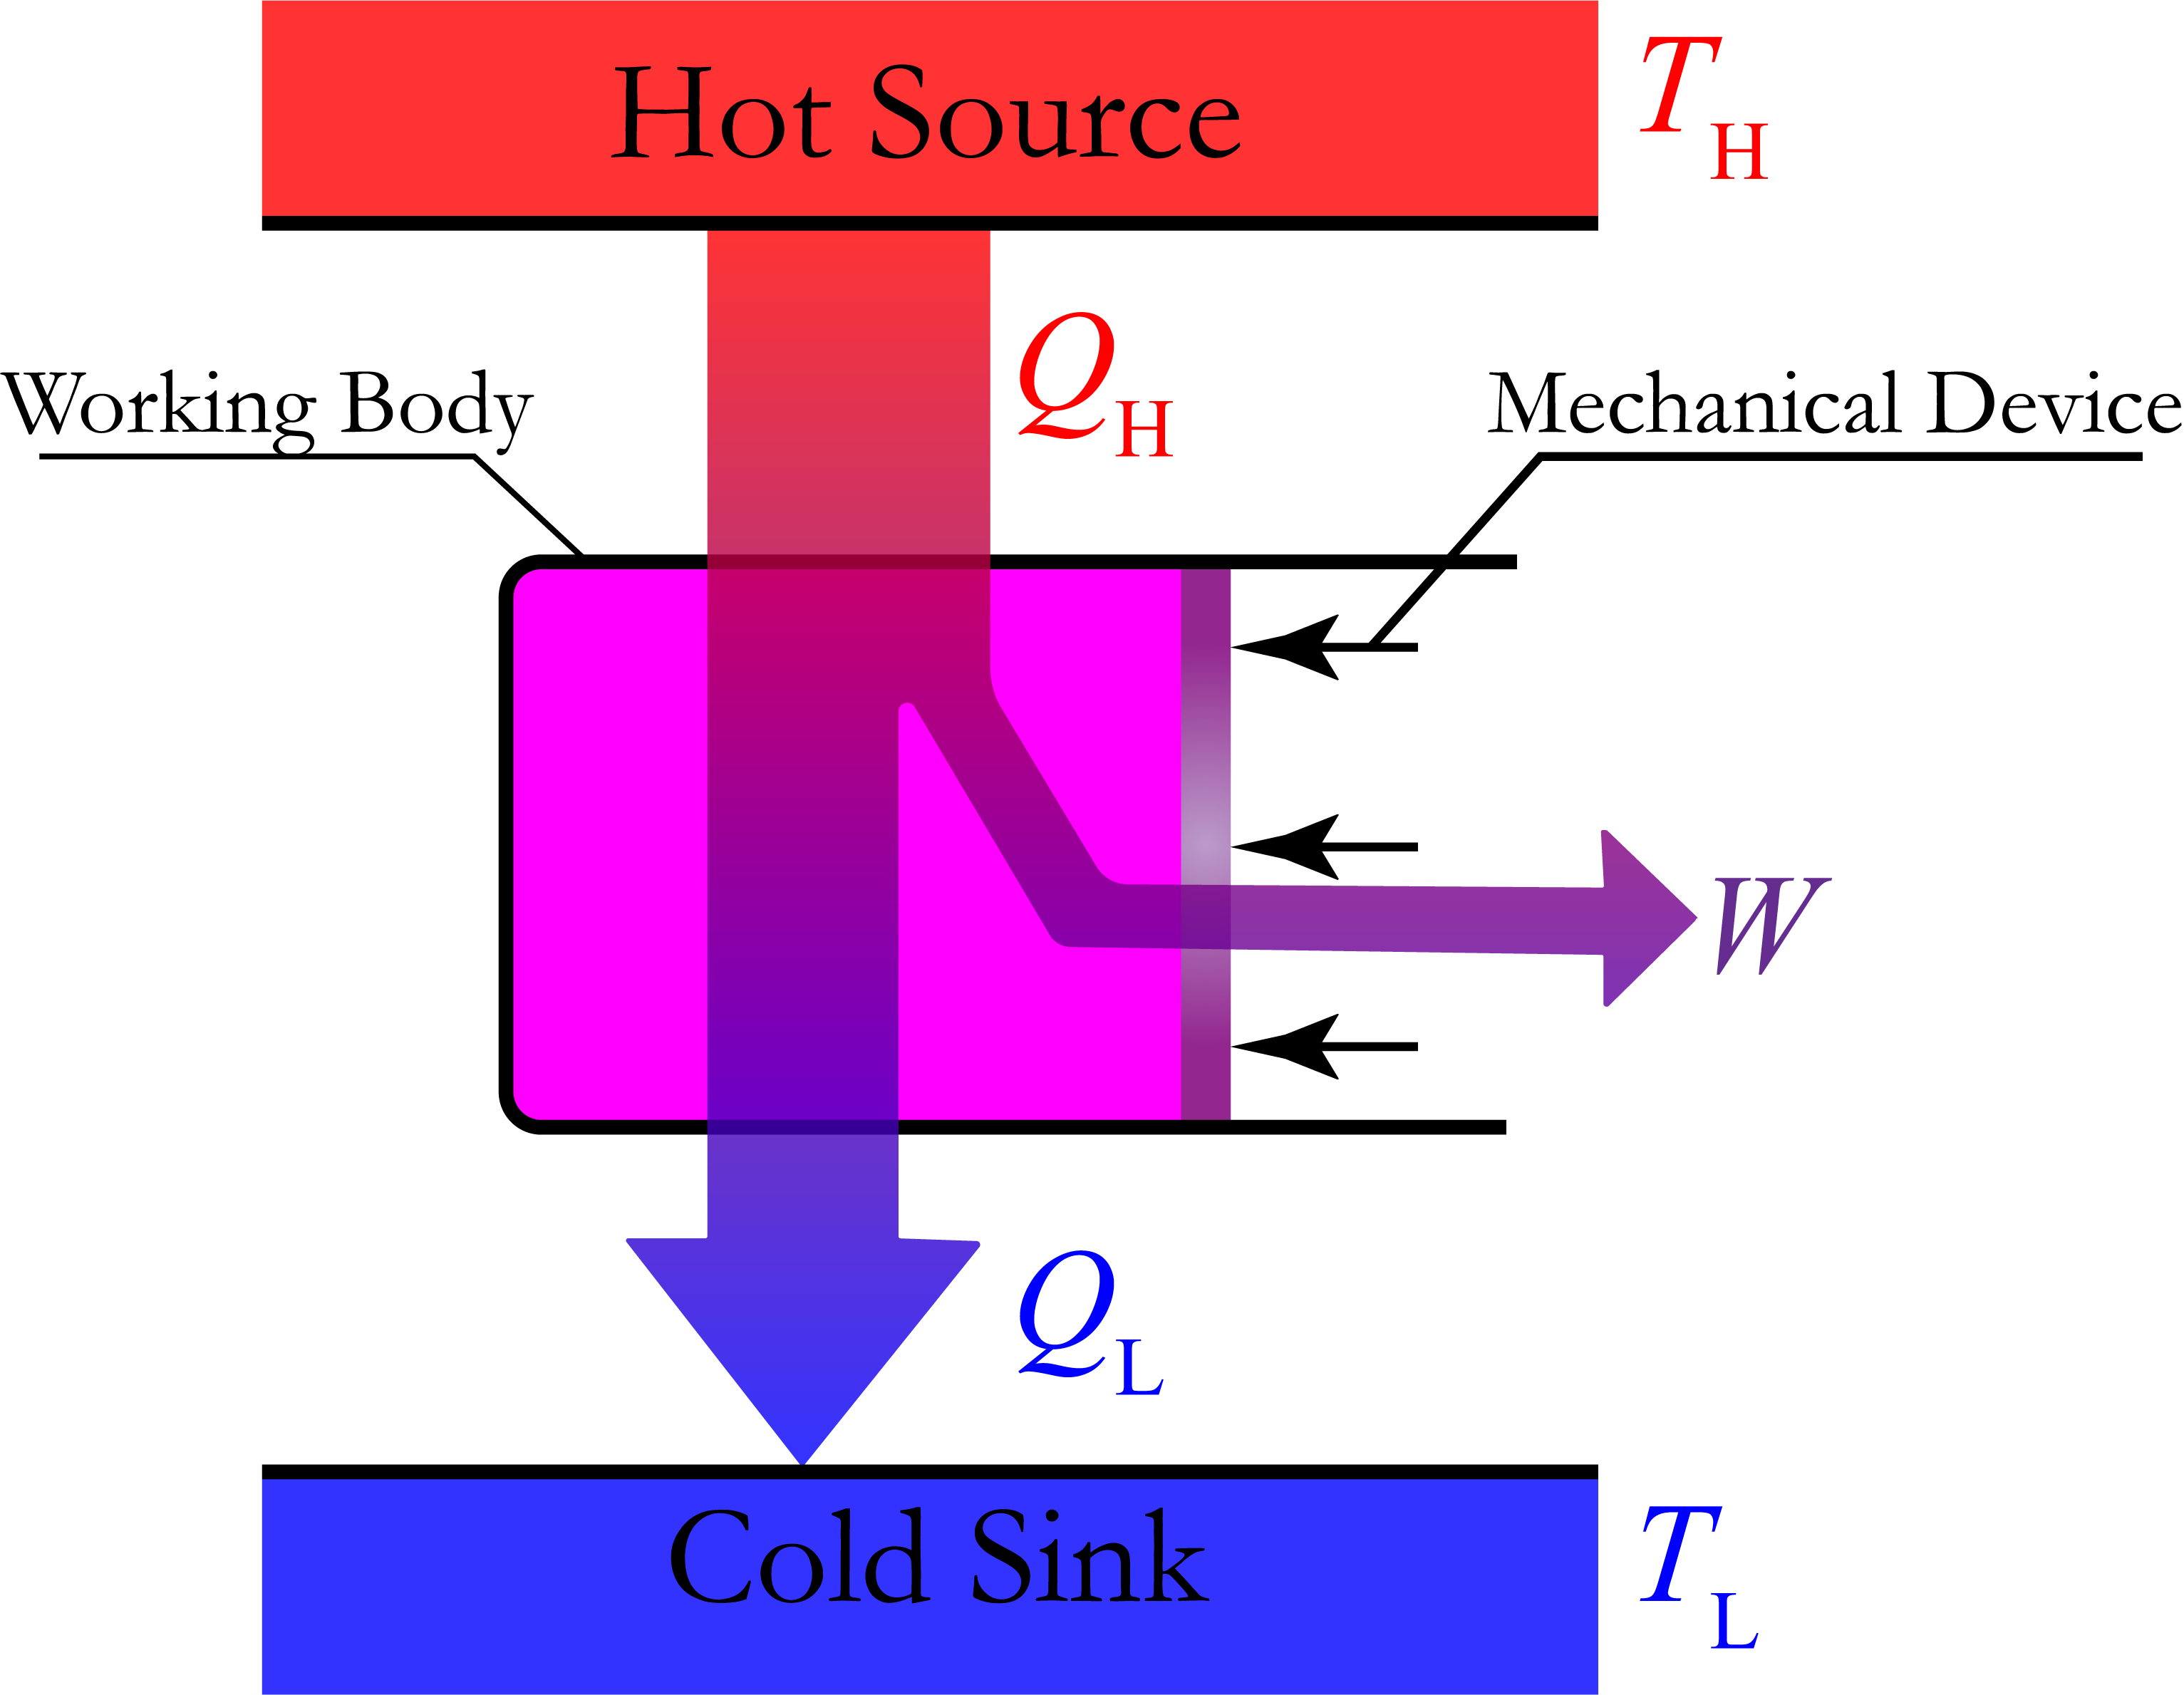
\includegraphics[width=7cm]{image/5-2-1.png}
\caption{热机模型}\label{fig:heat engine}
\end{wrapfigure}
上一章介绍过循环过程的概念.\,我们介绍了$p-V$系统的正负循环.\,现在我们把这样的$p-V$体系看成很多实际生活中一些机器的工作过程的抽象.\,其实际承担了状态循环变化的体系称为\emph{工作物质}(working body).\,而其联动的\emph{机械装置}(mechanical device)可以与外界交换功.\,最后,\,这样的体系还需要可以与其交换热量的对象,\,凡是工作物质从中吸热的被称为\emph{热源}(heat source),\,而工作物质向之放热的被称为\emph{冷库}(cold sink).\,这样我们就抽象出了一个理论模型,\,根据热力学第一定律,\,如果做正循环,\,工作物质一个循环将从高温热源吸收更多的热量,\,向低温冷库放更少的热量,\,而通过机械装置输出功,\,故被称为\emph{动力循环}(power cycle),\,对应机器为\emph{热机}(heat engine).\,而如果考虑相反的过程\footnote{这样的过程不一定可逆,\,这里指的是那些定性现象相反的循环.},\,工作物质一个循环向高温热源放热,\,从低温冷库吸热,\,机械装置要对它做功,\,则是一个\emph{泵热循环}(heat pump cycle).\,对应机器被称为\emph{热泵}(heat pump).

\begin{figure}[H]
\centering
\includegraphics[width=14cm]{image/5-2-2.jpg}
\caption{俄罗斯巴拉科沃(Balakovo)核电站汽轮机}
\end{figure}

根据以上原理,\,热机主要分为以下两大类:
\begin{description}
	\item[\hei 蒸汽机(steam engine)]  蒸汽机是一类\emph{外燃机}(external combustion engines),\,工作物质是在气相与液相混合的水(水蒸气).\,用外界燃烧的热量,\,或者来自太阳能,\,核能,\,地热等的非燃烧热量加热\emph{锅炉}(boiler)中的水,\,由此产生高温高压蒸汽,\,用蒸汽带动机械装置运转向外输出能量.\,经过这样的装置后(这中间一般视为节流过程),\,水蒸气一般变为过饱和的冷气体或者还夹杂着水滴,\,进一步导入冷凝器而液化变为液态水回收进入锅炉.\,完成一个循环.\,18世纪末与大半个19世纪可谓``蒸汽时代'',\,蒸汽机在大型机械生产工厂,\,蒸汽机车,\,蒸汽机轮船等交通工具中大放异彩.\,虽然石油开采为小型汽车生产提供了可能,\,大型交通工具和生产业动力来源之后也慢慢地几乎被内燃机与电力所取代.\,但直到今天,\,我们的生产生活有$90\%$以上的电量都来自于\emph{汽轮机}(steam turbine)形式的热电厂.\,值得一提的是其中化石能源(煤电,\,气电,\,以及较为小规模的油电)仍然占据$75\%$的高比重(中国与美国的情况大致相同),\,新型能源的比重不大,\,但在稳步上升中.
	\item[\hei 内燃机(internal combustion machine)]  蒸汽机的锅炉设计让燃烧能量给了流动的工作物质,\,实现了工作物质不含燃料,\,不与燃料混合或被燃料污染.\,这有效地提高了燃料能量利用的效率.\,然而却需要为工作物质准备额外的空间,\,不利于把热机做小.\,与之相反,\,内燃机利用了\emph{燃烧室}(combustion chamber)的设计,\,工作物质直接是高能量密度的燃料和氧化剂(一般就是空气).\,利用高温高压下点燃化学反应释放的巨大化学能来产生热,\,导致气体反向对机械装置\ca \emph{活塞}(piston)或\emph{涡轮}(rotor)做功.\,与外燃机工作物质发生的真循环过程不同,\,内燃机发生的过程是一种开放循环.\,以常规的四冲程活塞式内燃机为例,\,气体经历四个冲程:\,\emph{吸入}(intake),\,\emph{压缩}(compression),\,\emph{做功}(power),\,\emph{排出}(exhaust).\,整个循环从常态燃料中开始,\,最后以排出气体在大气中冷却结束.\,而\emph{燃气涡轮发动机}(gas turbine engine)更是针对四个阶段分别设计功能区,\,使得四个阶段同时进行,\,提供了极大的功率输出.\,按照其机械装置的不同分为四类:\,军用战斗机往往采用\emph{涡喷发动机}(turbojet engine),\,而民航客机往往是\emph{涡扇发动机}(turbofan engine);\,运输机,\,巡逻机经常采用\emph{涡桨发动机}(turboprop engine);\,而直升机和其他陆上,\,海上交通工具则通过\emph{涡杆发动机}(turboshaft engine)将动力用传动轴导出.\,在这样的设计中,\,燃料产生的能量用来驱动涡轮带动整个装置大量吸入外界空气\footnote{火箭除外,\,它需要自备燃料与氧化剂.}并有效地压缩气体从而产生动力.\,涡轮转动的能量也正是很多民航飞机上电力的来源.
\end{description}
\begin{figure}[H]
\centering
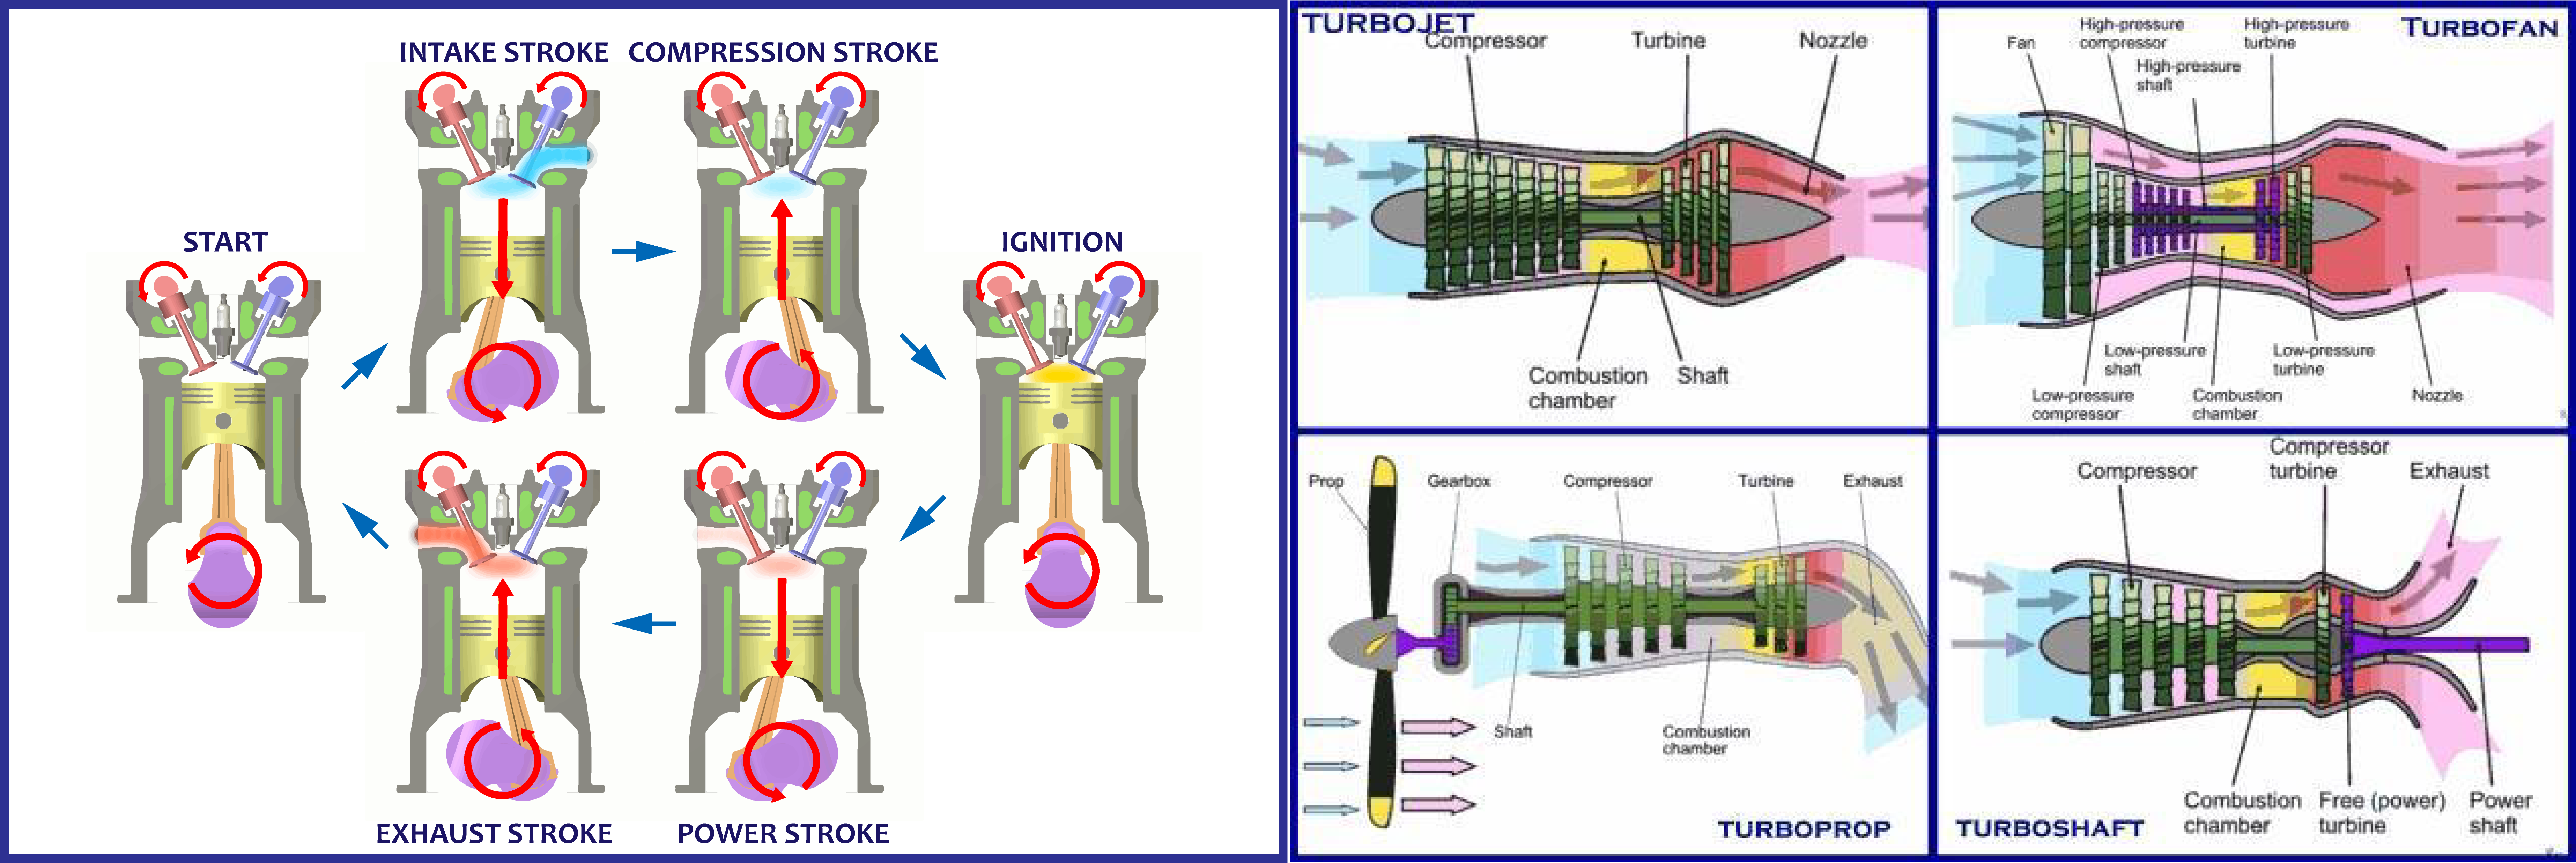
\includegraphics[width=17cm]{image/5-2-3.png}
\caption{左:\,四冲程活塞内燃机;\,右:\,四类涡轮机}
\end{figure}

我们发现,\,将实际的热机抽象为前图\ref{fig:heat engine}那样的模型往往是过分地简单了.\,实际问题中的工作物质往往成分在发生改变,\,有物质的输入输出,\,甚至无法视为一个完整的循环过程.\,但理论可以帮我们分析与把握这个过程的一些主要信息.\,在实际问题中热机的\emph{能效}(energy efficiency)是主要的关心因素之一,\,它定义为输出的有用功$W$与燃料提供的化学能$Q_{\rm H}$之比:
\[\eta=\frac{W}{Q_{\rm H}}\]

\begin{wrapfigure}[22]{o}[-10pt]{7cm}
\centering
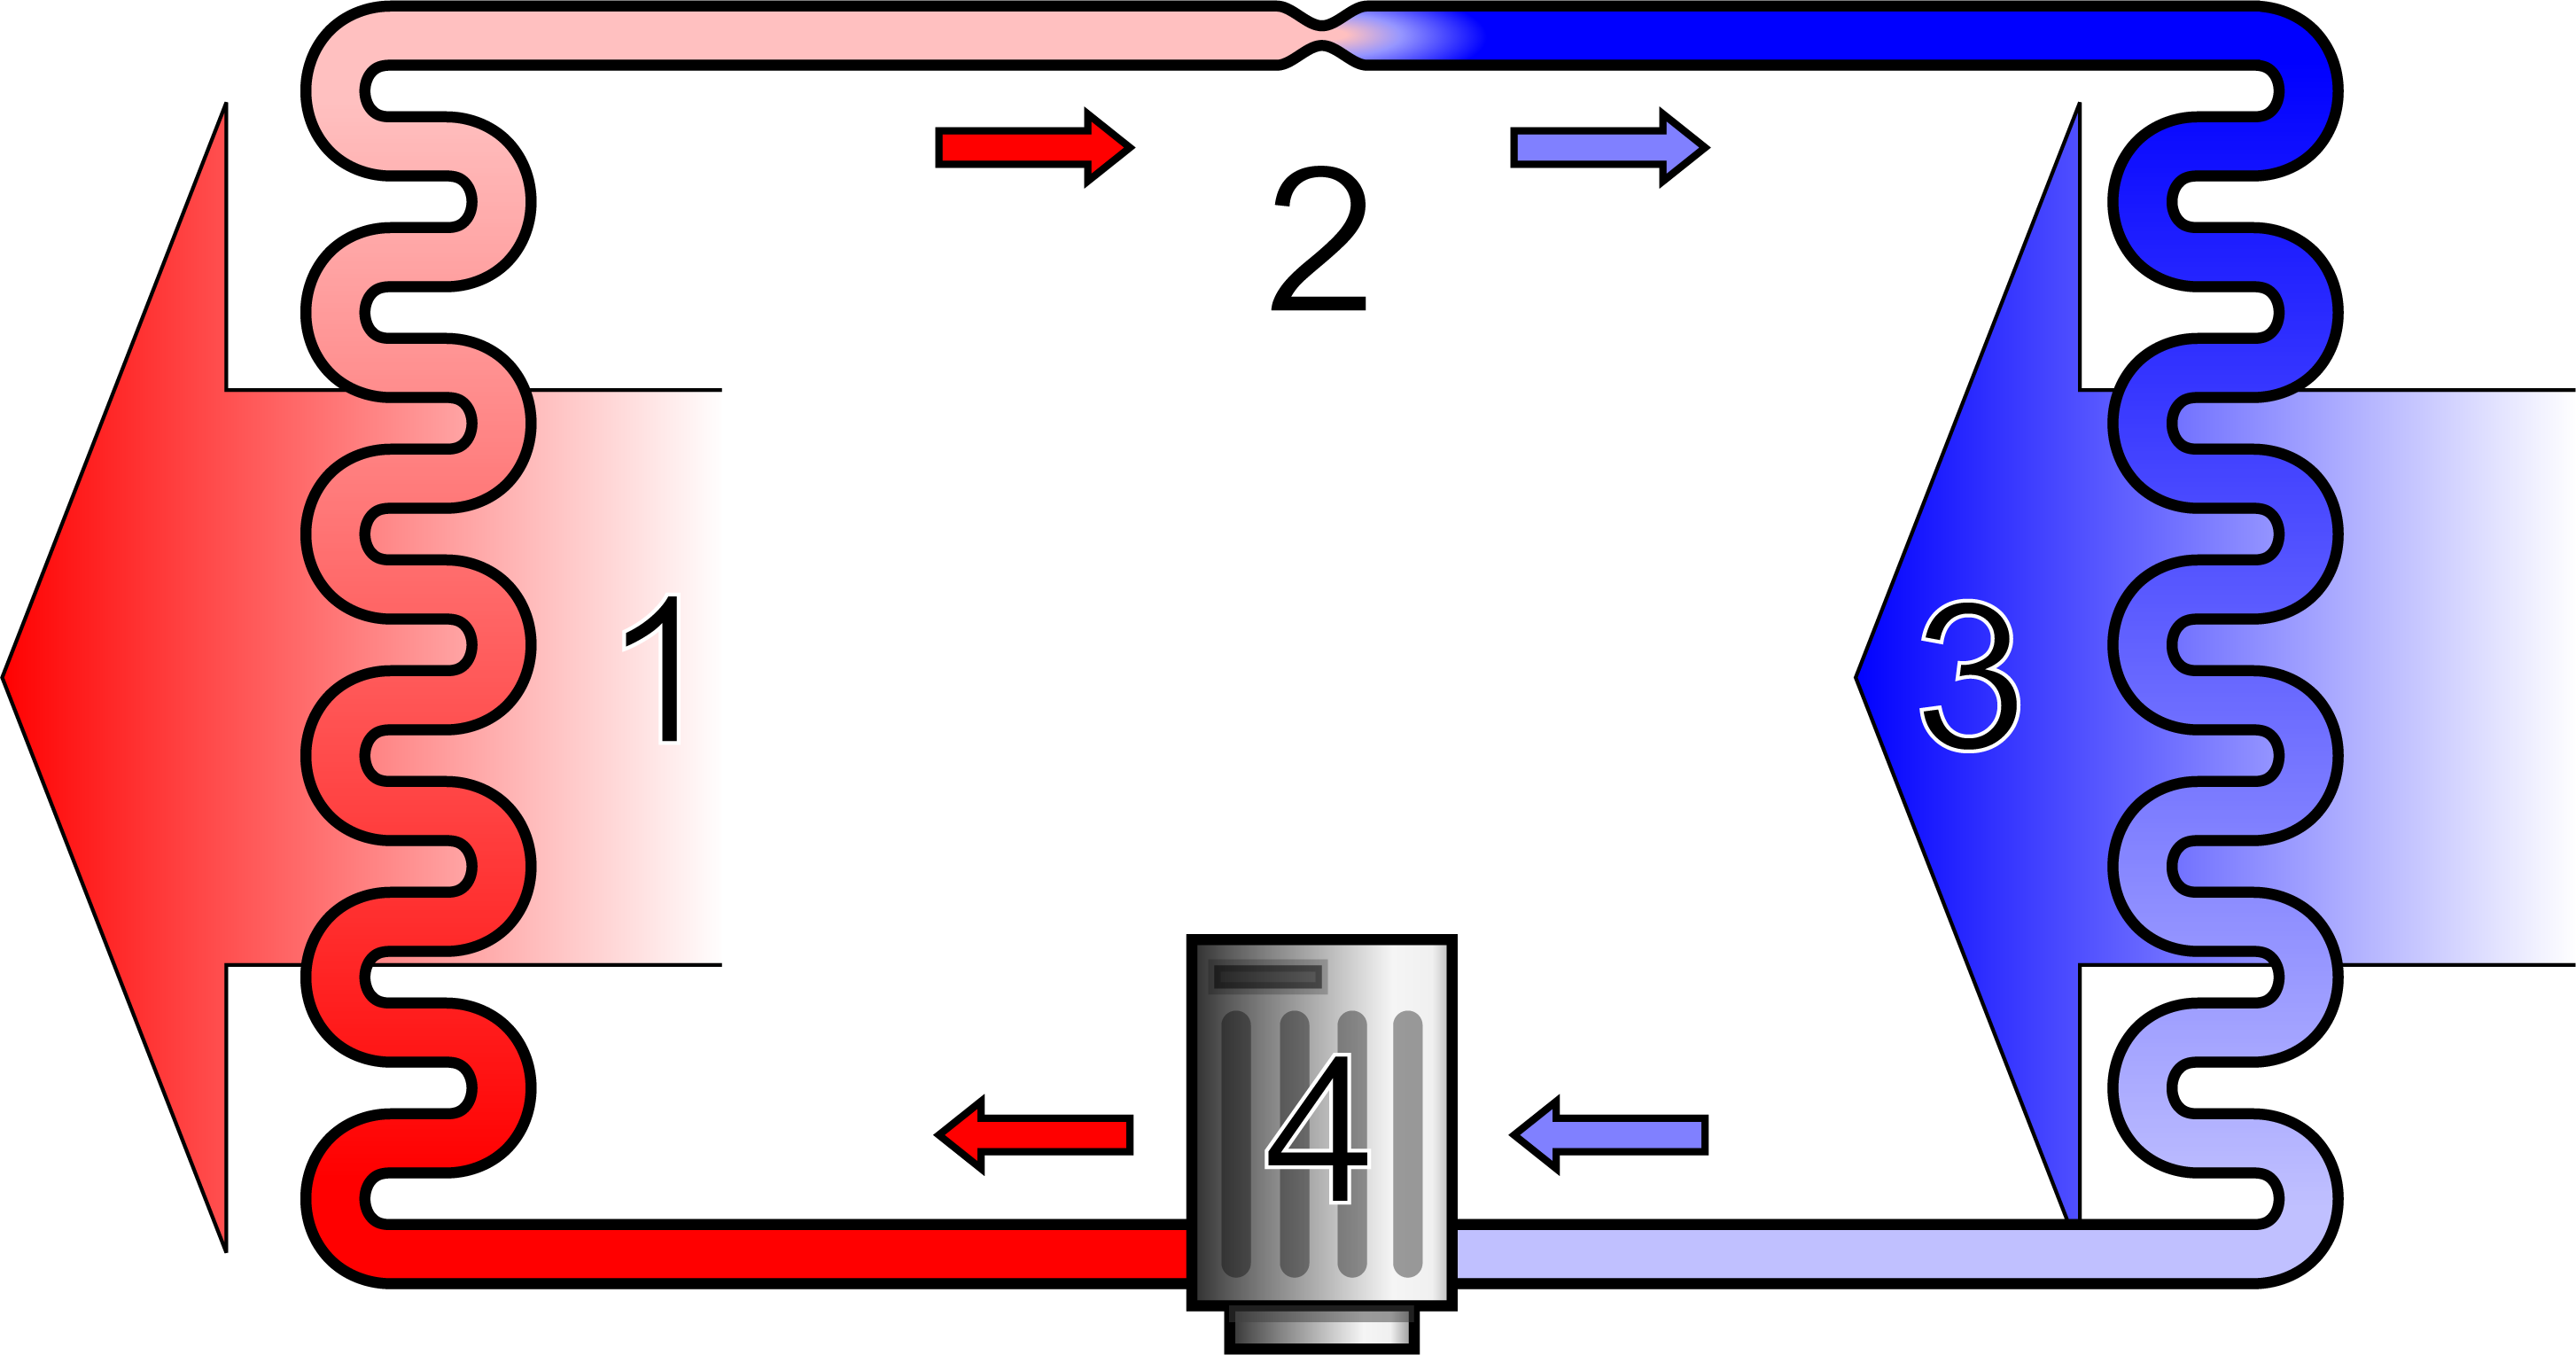
\includegraphics[width=7cm]{image/5-2-4.png}
\caption{热泵的普遍构成}
\vspace{1cm}
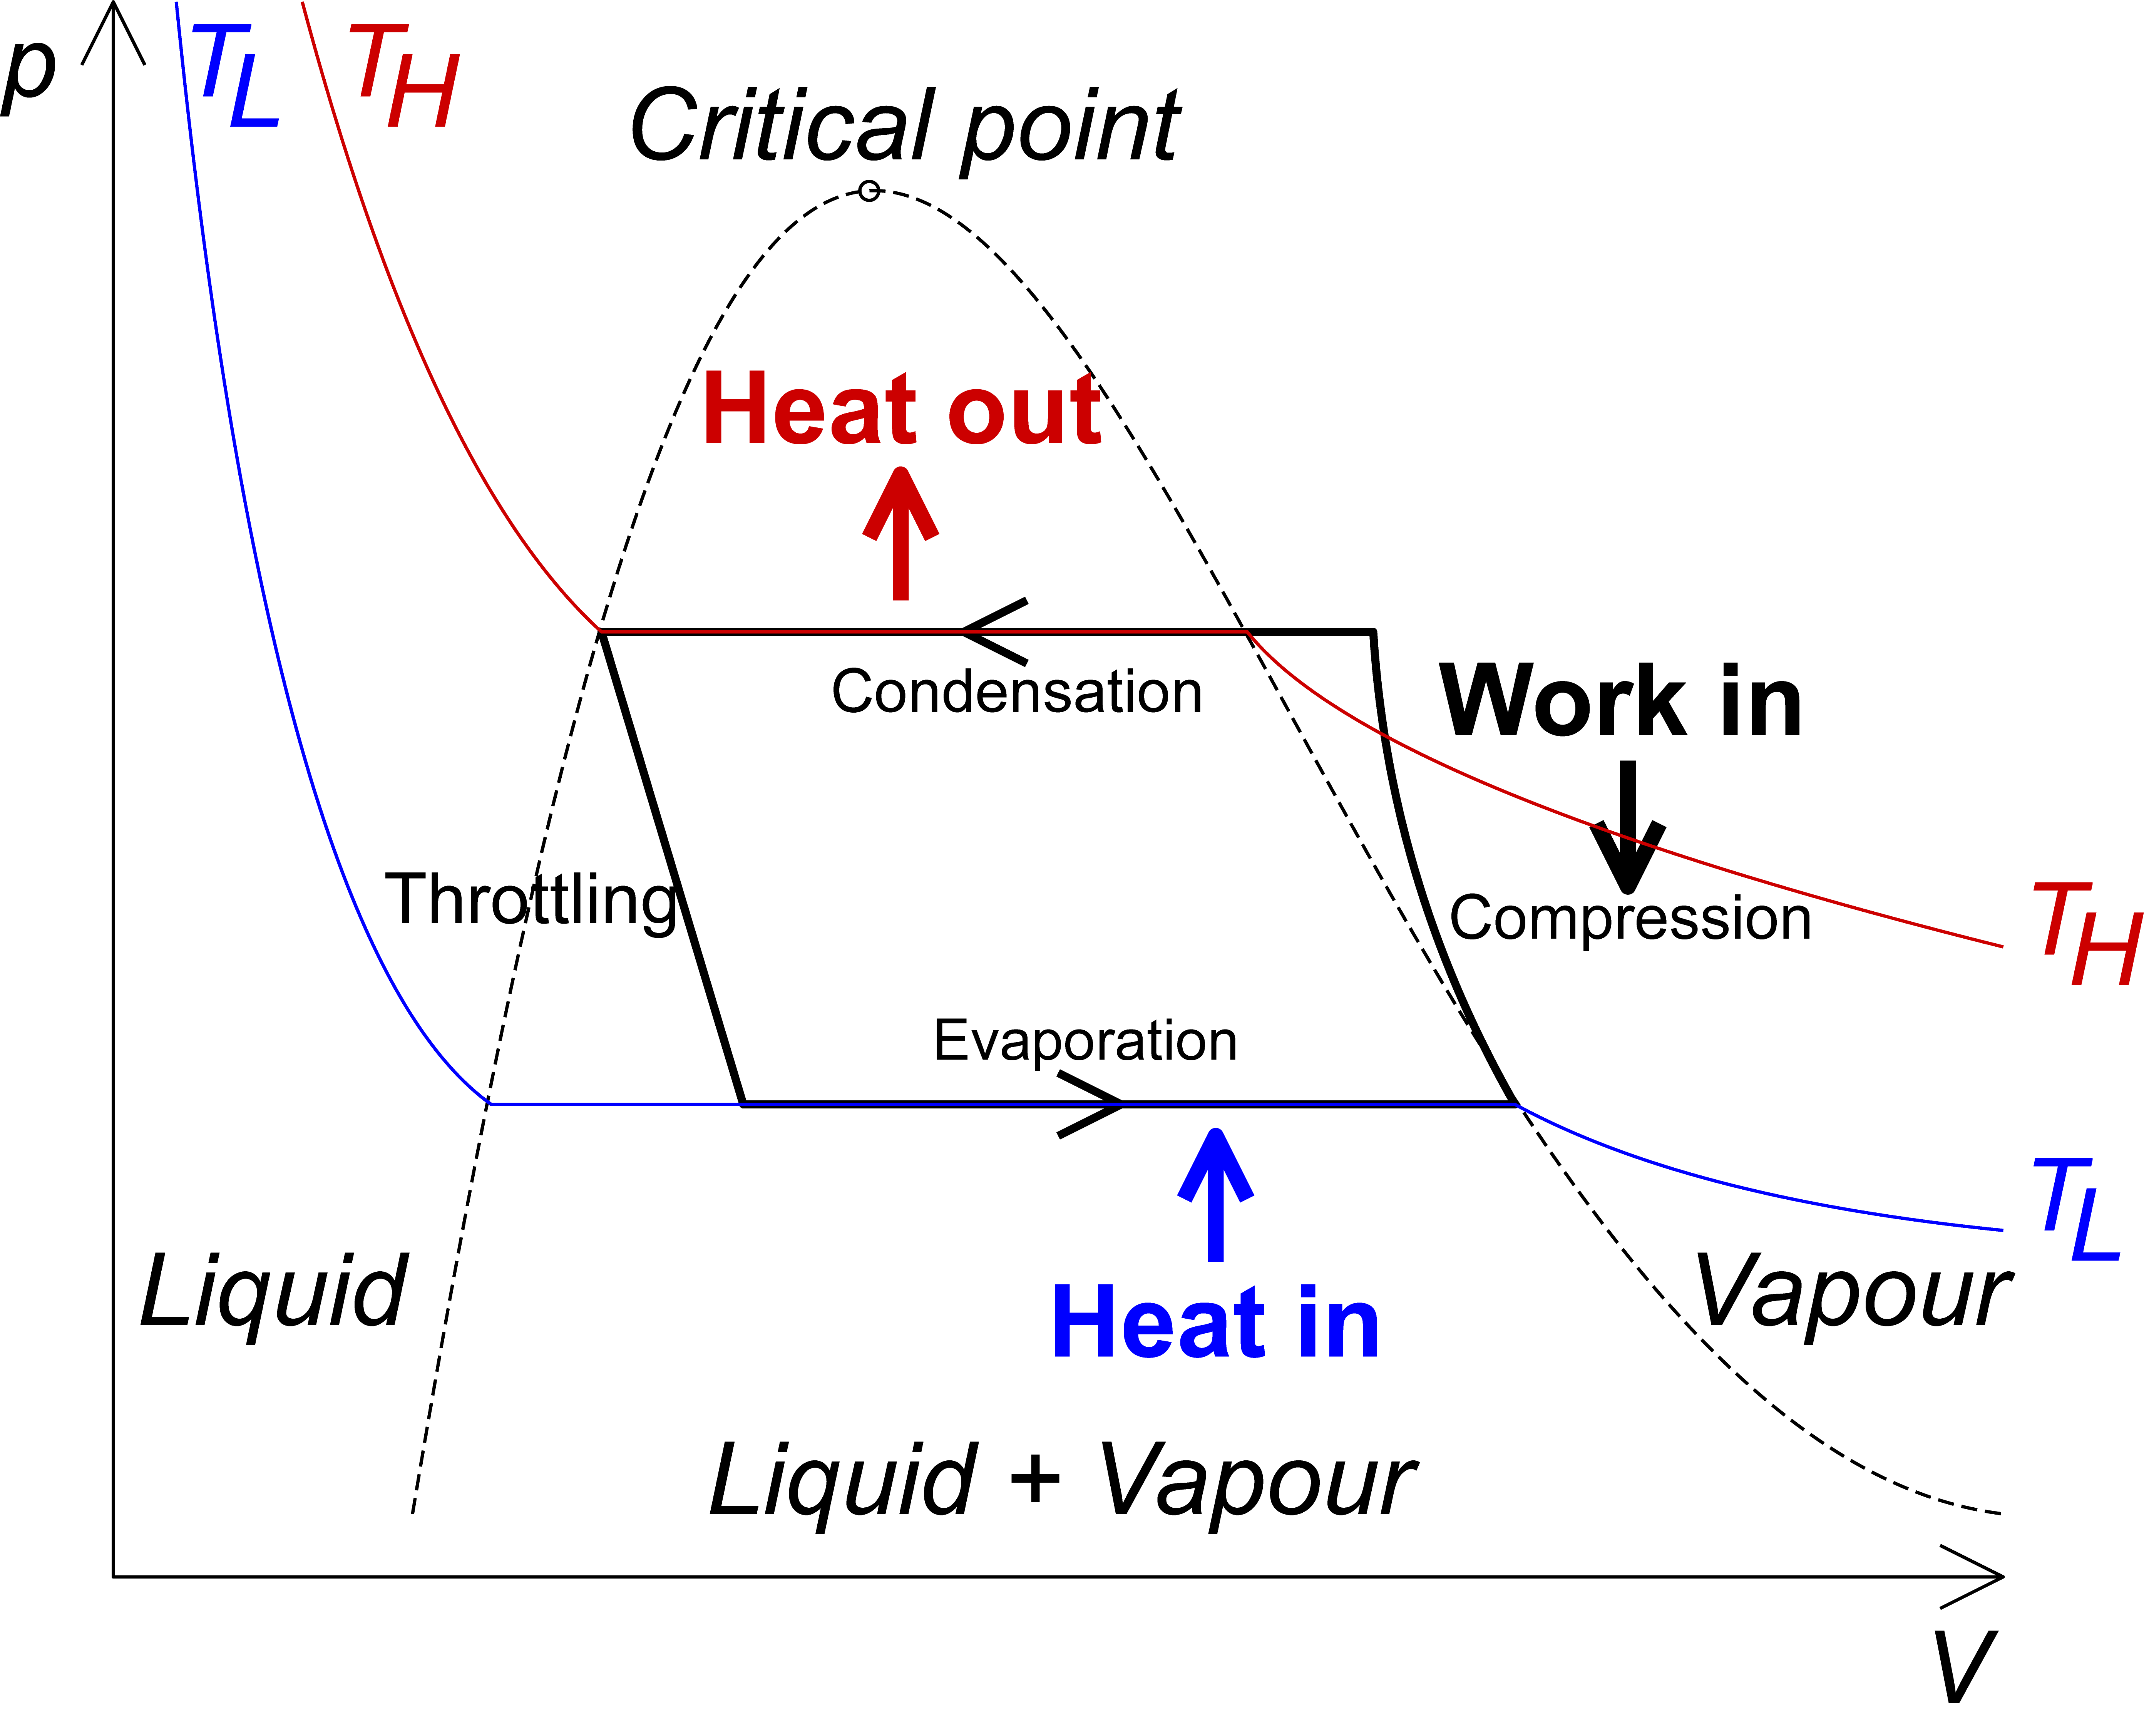
\includegraphics[width=7cm]{image/5-2-5.png}
\caption{热泵的工作循环}
\end{wrapfigure}
而热泵也根据其设计功能分为\emph{制冷机}(cooling machine),\,\emph{制热机}(heating machine)与\emph{可逆机}(reversible machine).可逆的热泵同时具备制冷制热两种功能,\,采用换向阀来控制气流的流向从而改变效果.\,当采用制热模式时,\,其效率往往比使用单独的电阻加热高3到4倍.

无论何种类型的热泵,\,其构成与原理可以被抽象为典型的四步.\,高温热源处更高温的气体在\emph{冷凝器}(condenser)处变为液态而放热;\,\emph{膨胀阀}(expansion valve)处的节流过程使液态流体温度与压强大降而成为气液混合的状态;\,低温冷库处稀薄的半液态流体在\emph{蒸发器}处蒸发吸热;\,最后通过\emph{压缩机}(compressor)泵入冷凝管,\,压强与温度显著升高.\,这样的循环称为\emph{斯特林循环}(Stirling cycle).


而对于热泵的\emph{性能系数}(coefficient of performance),\,需要对两种不同的模式区分:

对于制冷模式,\,取低温冷库处吸热比输入功率:
\[\eta=\frac{Q_{\rm L}}{W}\]

对于制热模式,\,取高温热源处放热比输入功率:
\[\eta=\frac{Q_{\rm H}}{W}\]

两者都可能大于一.

\subsection{热机循环}
从瓦特({\it Watt}\,)改良蒸汽机开始,\,一代代的工程师开始致力于提高热机的效率.\,这其中便产生了大量实用的热机模型.\,直到1824年法国物理学家与工程师卡诺({\it Carnot}\,)给出了惊人的卡洛热机模型与关于热机工作效率上限的论断.\,这实际上意味着\emph{热力学}(thermodynamics)的诞生.\,之后热机优化建立在严格的热力学计算的基础上.\,发展到今天理论早已成熟,\,只待技术的发展与革新.

简单的热机循环计算往往将工作物质视为理想气体在$p-V$图上的准静态过程构成的循环.\,下将一一列举:
\subsubsection{\hei 勒鲁瓦循环(Lenoir cycle)}
\begin{wrapfigure}[11]{o}[-10pt]{5cm}
\centering
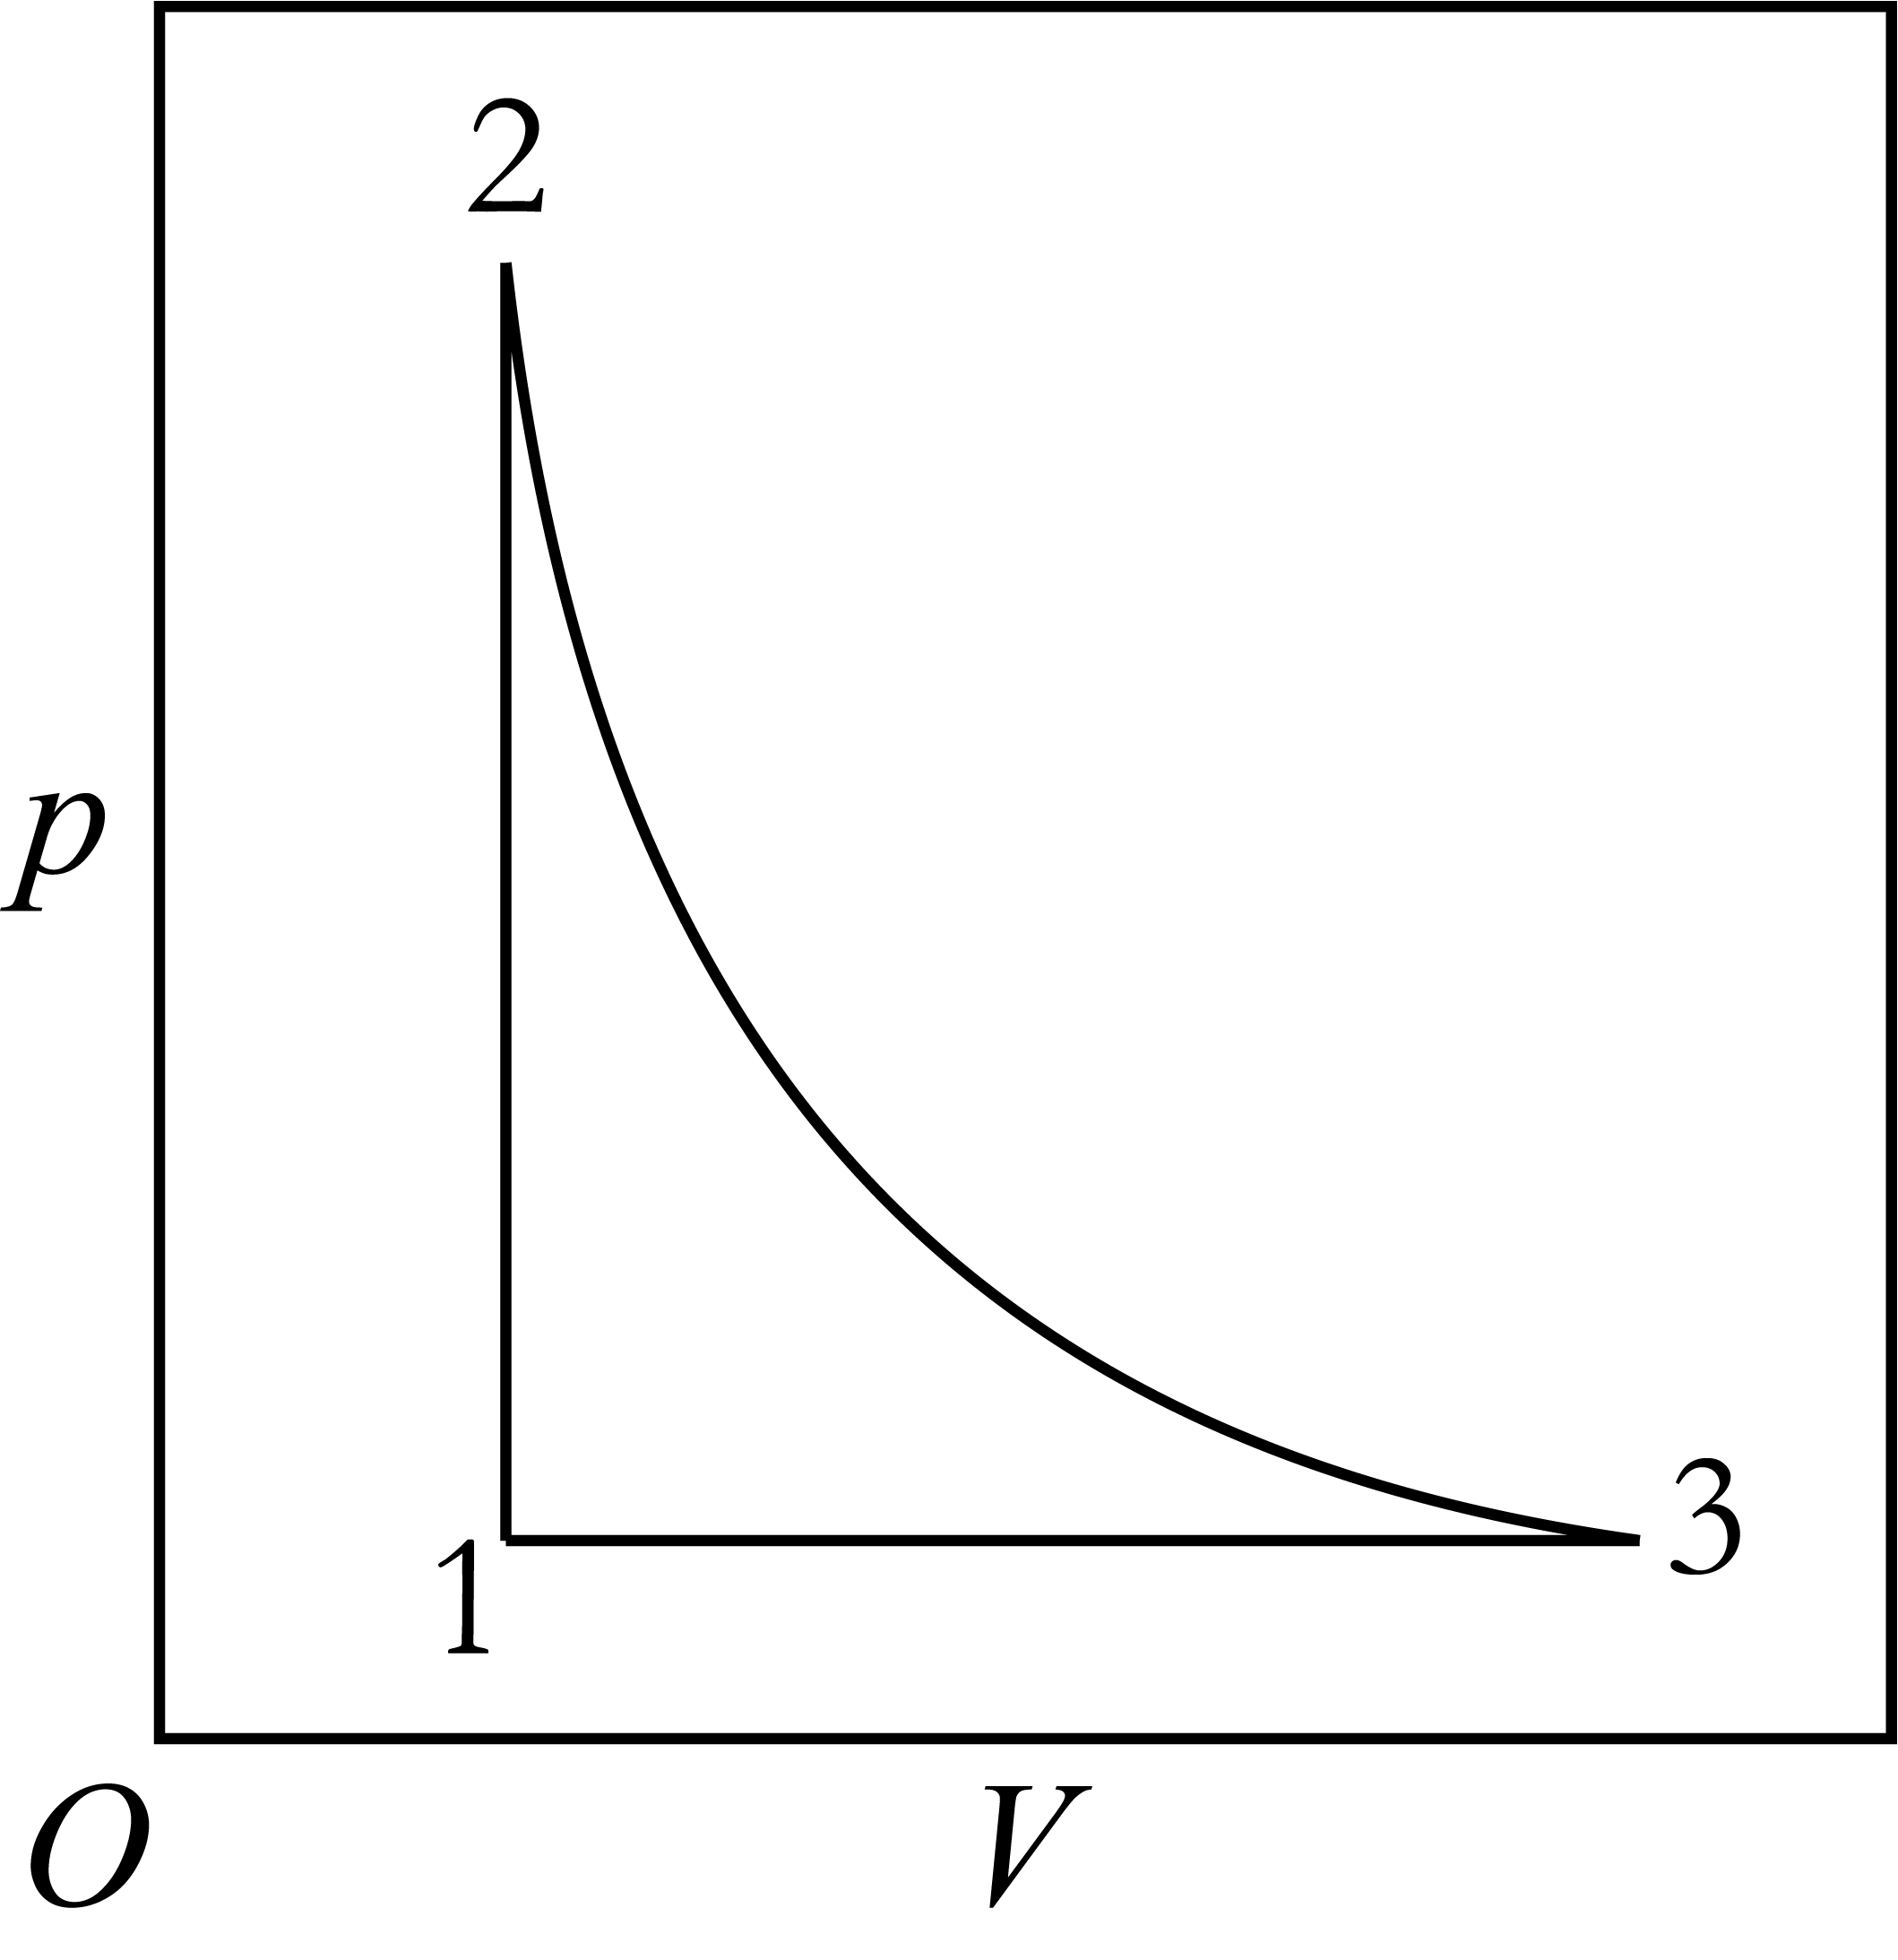
\includegraphics[width=5cm]{image/5-2-6.png}
\caption{Lenoir cycle}
\end{wrapfigure}
1860年法国工程师勒鲁瓦发明的勒鲁瓦机是第一个为商业设计的内燃机.\,其对应循环常常用来描述\emph{脉冲喷气发动机}(pulse jet engine)的模型.\,它区别于其他热机的特点是无需压缩气体.\,一个循环内,\,理想气经历:
\begin{enumerate}[i]
	\item 1-2:\,定容爆炸吸热
	\item 2-3:\,绝热膨胀
	\item 3-1:\,定压放热
\end{enumerate}

定义\emph{爆炸比}(explosion ratio)$r_p$:
\[r_p=\frac{p_2}{p_1}\]

则可以计算出其效率为:
\[\eta=1-\gamma\frac{T_3-T_1}{T_2-T_1}=1-\gamma\frac{r_p^{\frac{1}{\gamma}}-1}{r_p-1}\]
\subsubsection{\hei 奥托循环(Otto cycle)}
\begin{wrapfigure}[12]{o}[-10pt]{5cm}
\centering
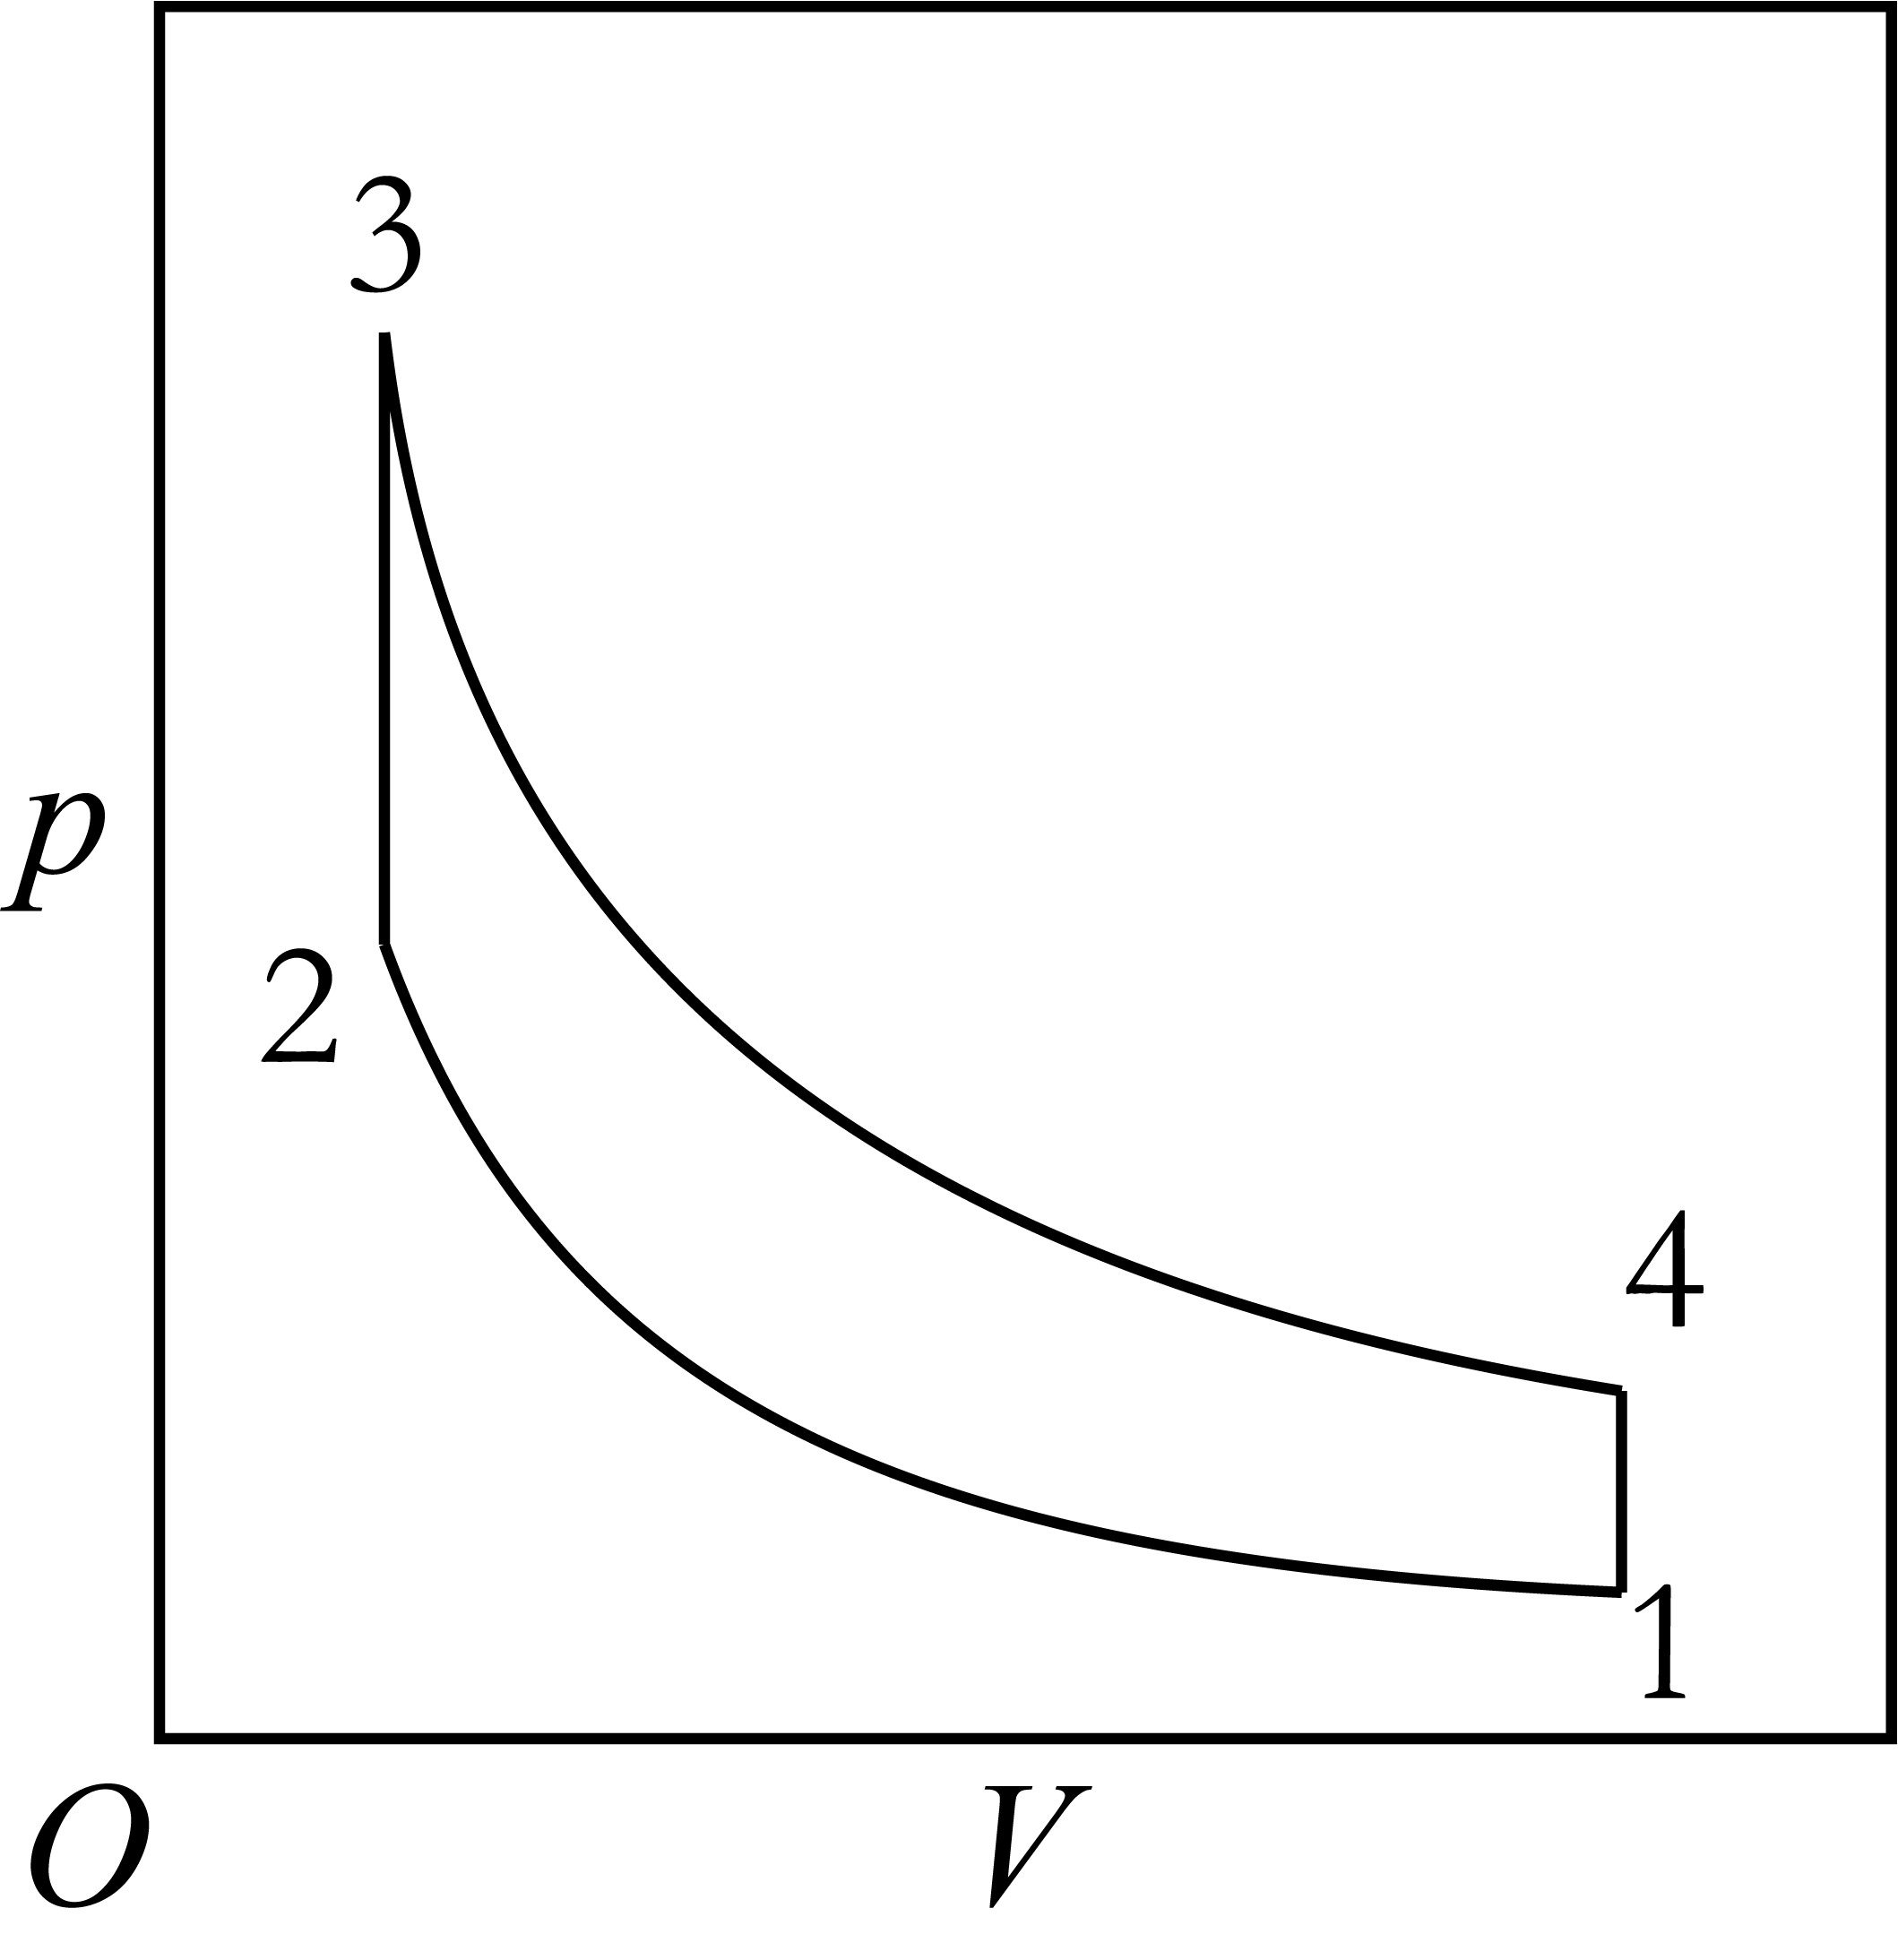
\includegraphics[width=5cm]{image/5-2-7.png}
\caption{Otto cycle}
\end{wrapfigure}
这是最典型的四冲程型\emph{汽油机}(gasoline engine,\,gas engine)的工作循环.\,特点是通过压缩气体产生高温高压易燃汽油空气混合体,\,再通过火花塞点燃混合体,\,过程可以视为瞬间发生的,\,从而体积不变,\,压强突然增大.\,一个循环内,\,理想气经历:
\begin{enumerate}[i]
	\item 1-2:\,绝热压缩
	\item 2-3:\,定容爆炸吸热
	\item 3-4:\,绝热膨胀
	\item 4-1:\,定容放热
\end{enumerate}

定义\emph{压缩比}(compression ratio)$r$:
\[r=\frac{V_1}{V_2}\]

则可以计算出其效率为:
\[\eta=1-\frac{T_1}{T_2}=1-\frac{T_4}{T_3}=1-r^{-(\gamma-1)}\]

对于空气与燃油的混合气$\gamma\simeq 1.3$,\,由于爆炸燃烧机制,\,目前的压缩比能做到$r\simeq 10$,\,这样看其理论效率上限$\sim 50\%$,\,目前一般的汽油机效率为$25\%\sim35\%$.\,最高能到$40\%$,\,离理论上限还尚有一段提升空间.

\npg{0cm}

\vspace{1cm}

\subsubsection{\hei 迪塞尔循环(Diesel cycle)}

迪塞尔机又称为\emph{柴油机}(Diesel fuel engine).\,其与汽油机设计上存在区别.\,为了提高汽油机的效率,\,柴油机企图增大压缩比,\,故采用粗重的活塞.\,并取消汽油机中点火爆炸的过程,\,而让压缩冲程的末温直接使得燃料能够燃烧,\,而缓慢注入燃料以使得燃烧充分.\,这样,\,典型的迪塞尔循环可以认为是这样四个过程:
\begin{wrapfigure}[12]{o}[-10pt]{5cm}
\centering
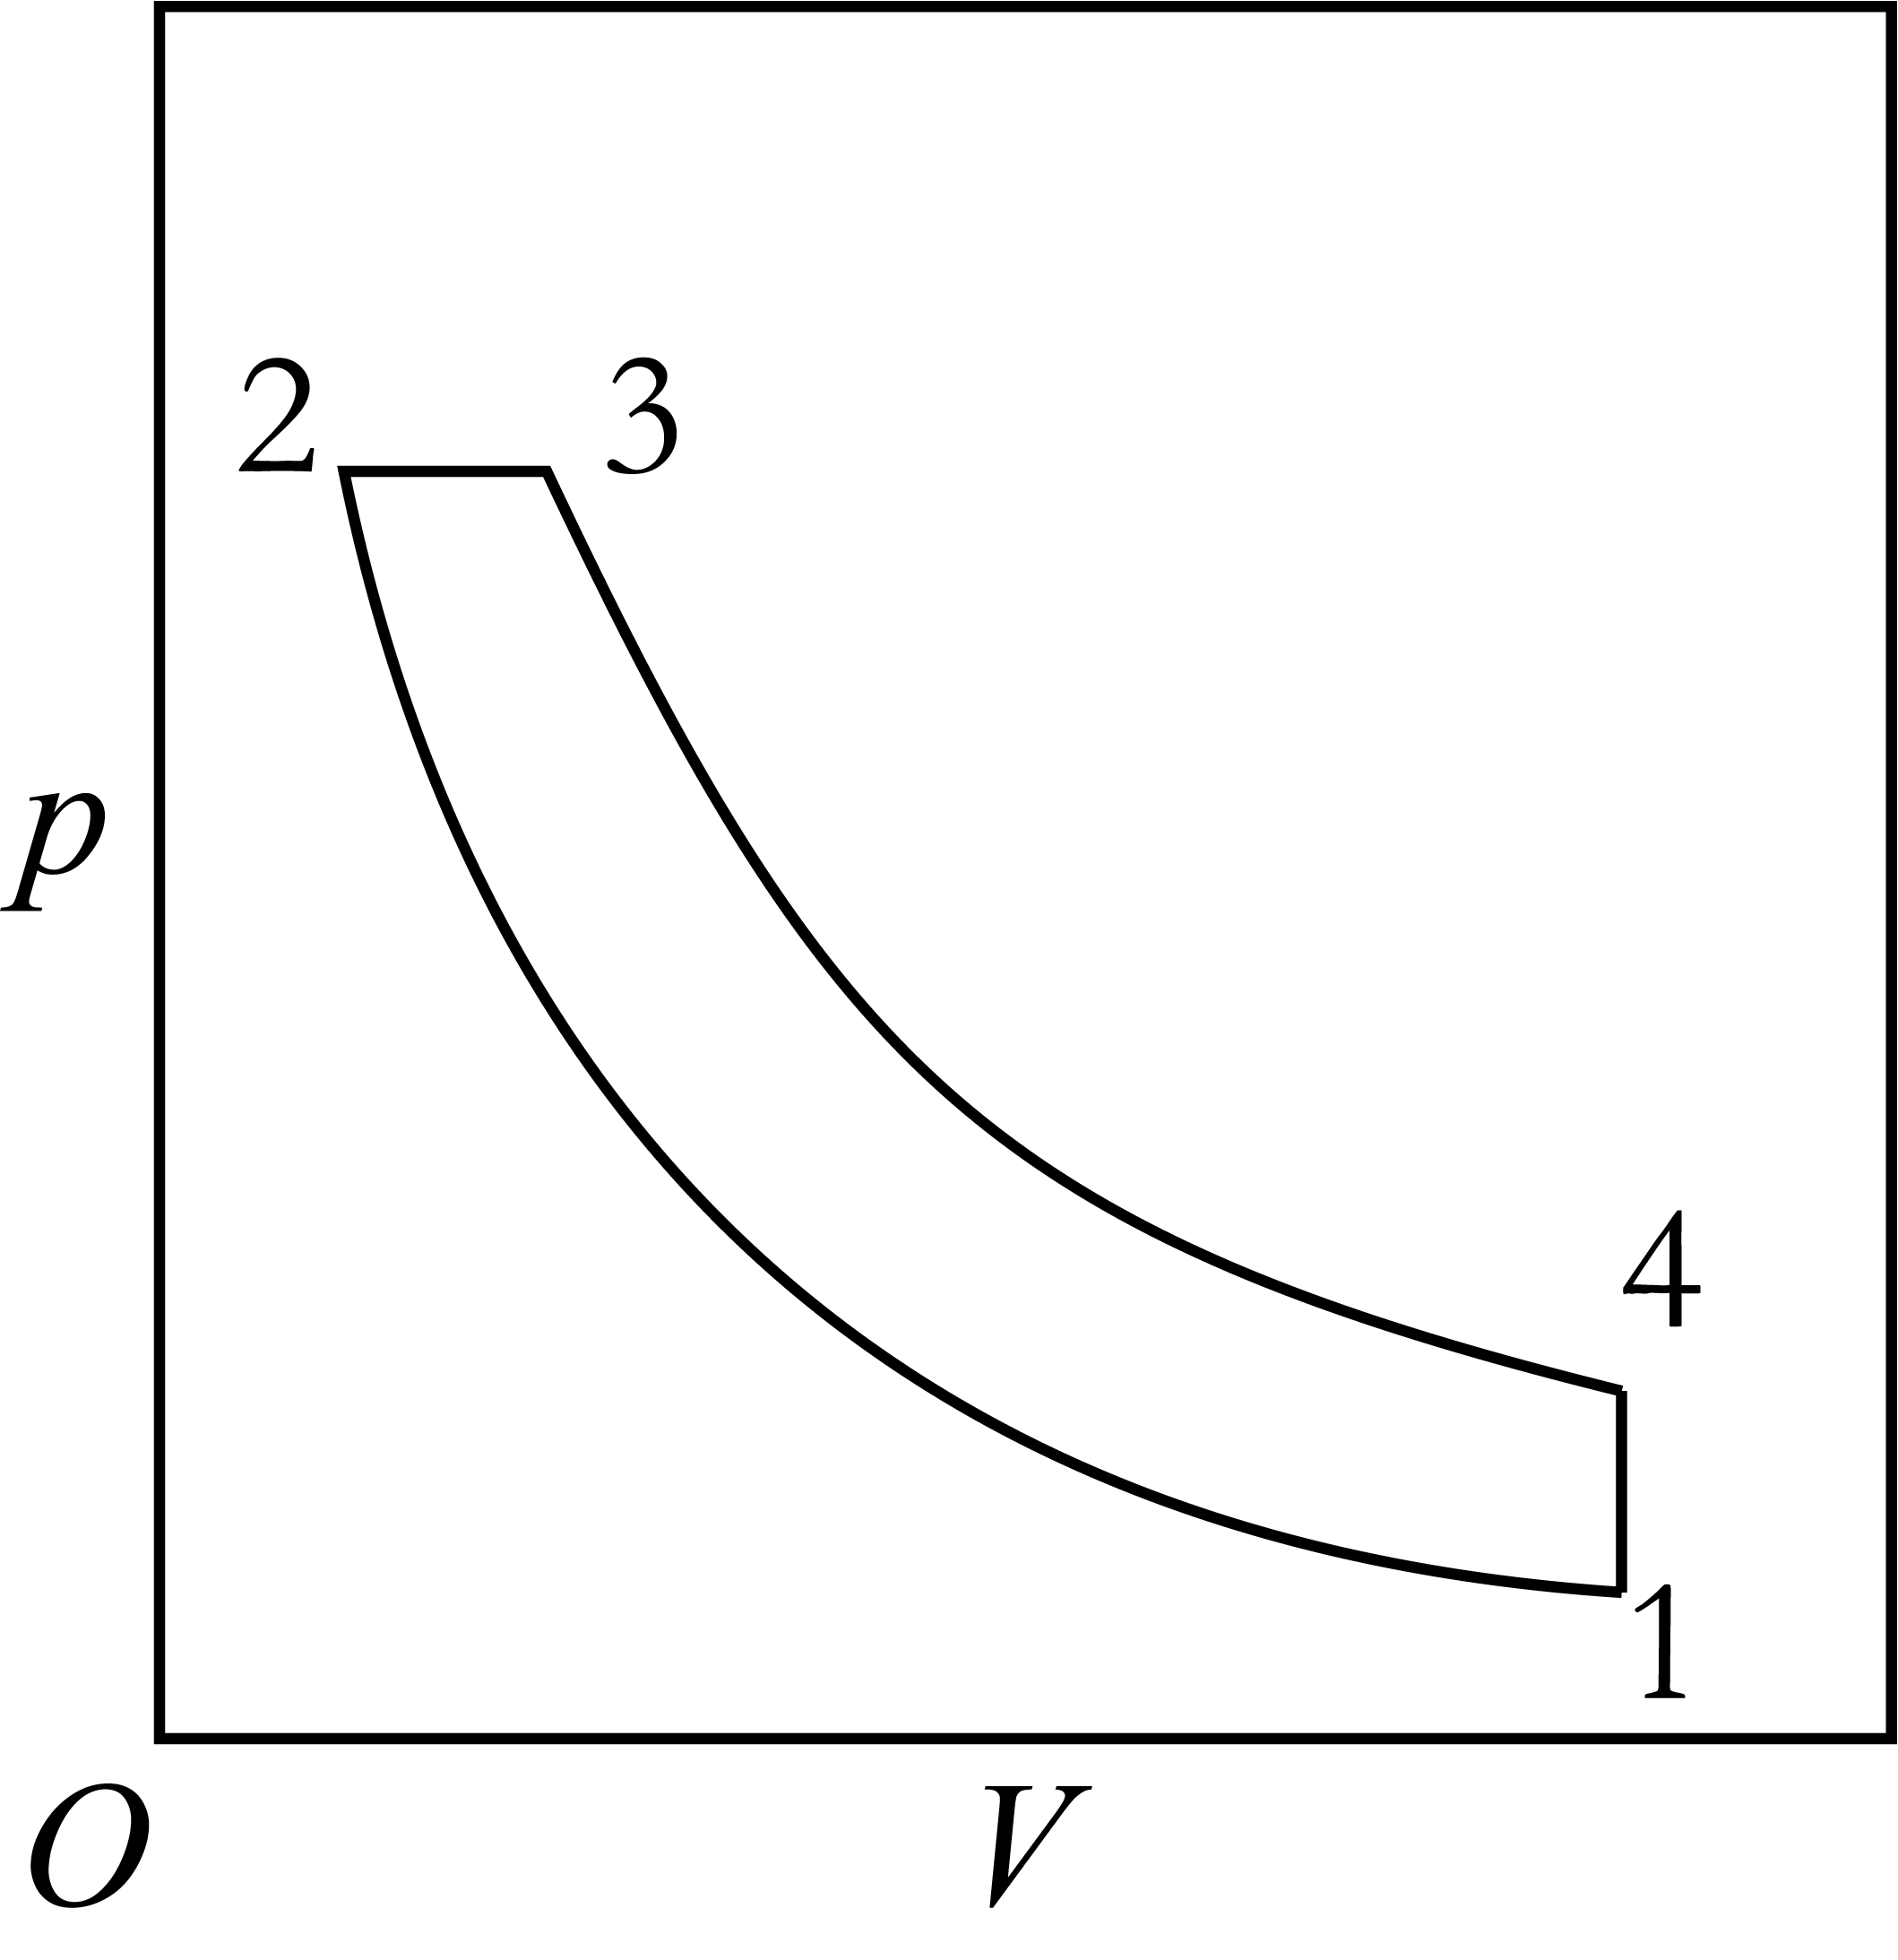
\includegraphics[width=5cm]{image/5-2-8.png}
\caption{Diesel cycle}
\end{wrapfigure}
\begin{enumerate}[i]
	\item 1-2:\,绝热压缩
	\item 2-3:\,定压燃烧吸热
	\item 3-4:\,绝热膨胀
	\item 4-1:\,定容放热
\end{enumerate}

定义压缩比$r$与\emph{停气比}(cut off ratio)$\alpha$:
\[r=\frac{V_1}{V_2}\quad ;\quad \alpha=\frac{V_3}{V_2}\]

则可以计算出其效率为:
\[\eta=1-\frac{1}{\gamma}\cdot\frac{T_4-T_1}{T_3-T_2}=1-\frac{\alpha^\gamma-1}{\gamma r^{\gamma-1}(\alpha-1)}\]

\vspace{2cm}

\subsubsection{\hei 布莱顿循环(Brayton cycle)}

涡轮机等开放式热力学循环的一般抽象是带有两个等压过程的布莱顿循环.\,可以认为是这样四个过程:
\begin{wrapfigure}[12]{o}[-10pt]{5cm}
\centering
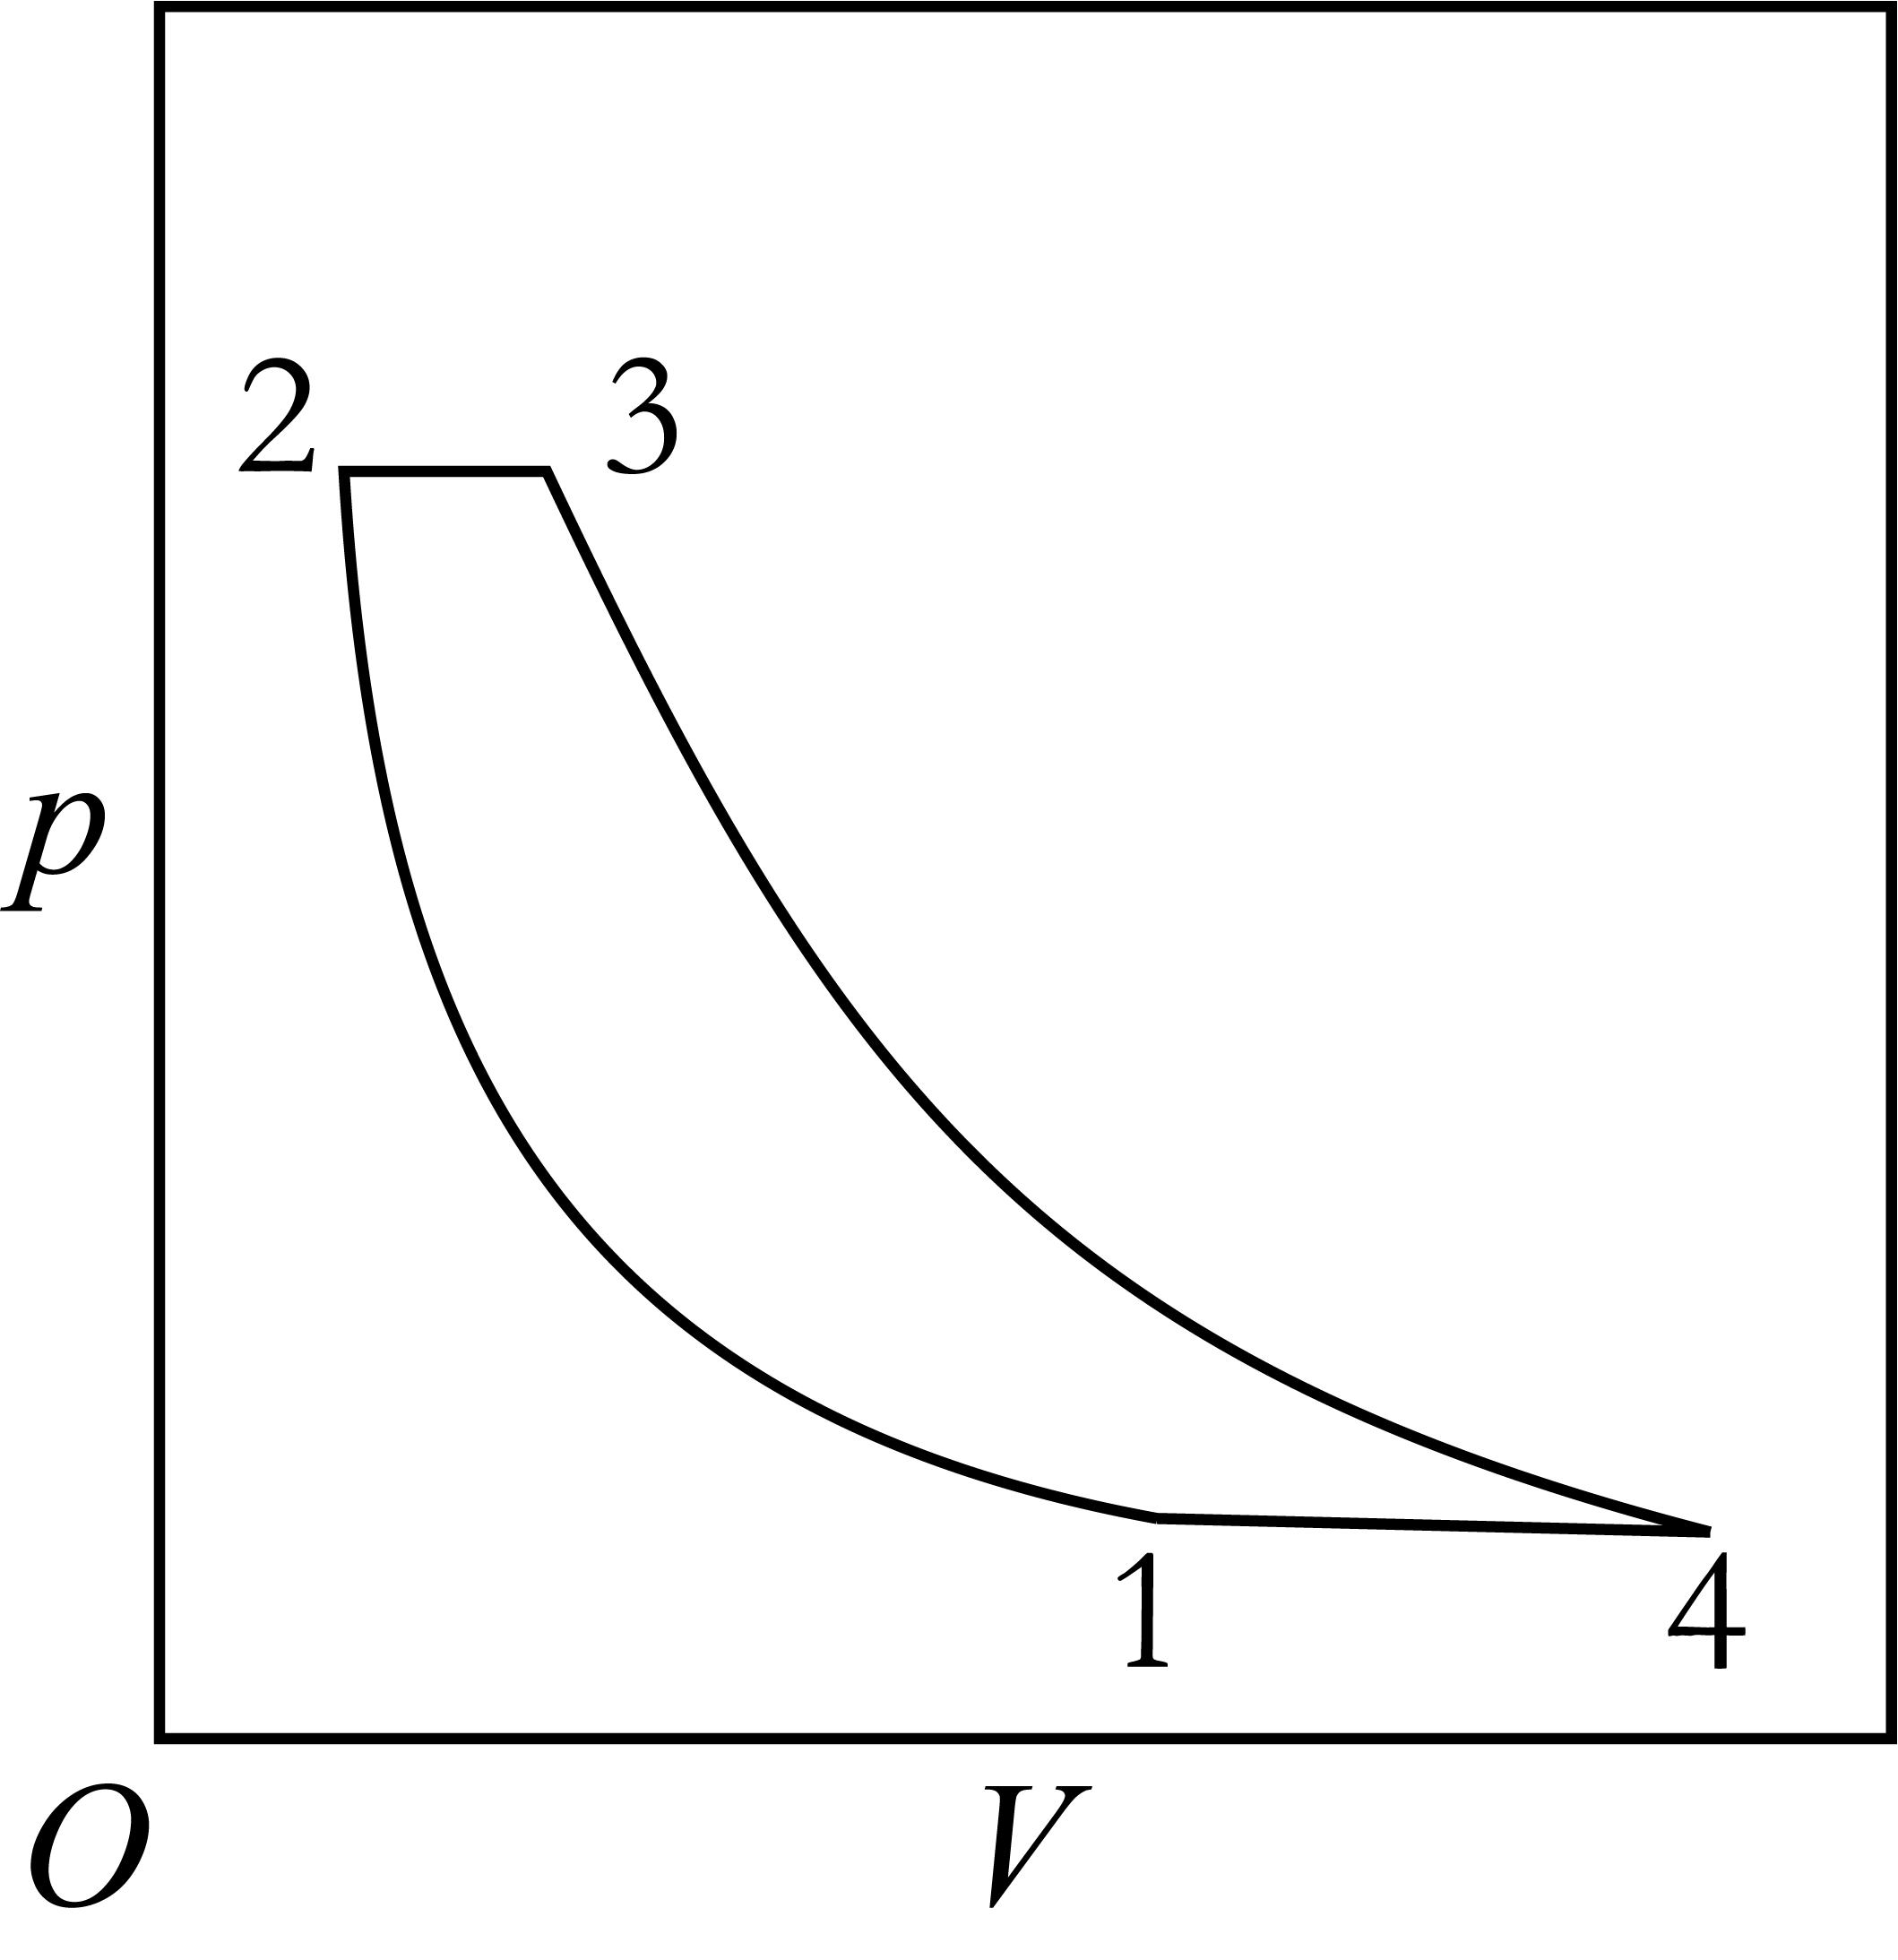
\includegraphics[width=5cm]{image/5-2-9.png}
\caption{Brayton cycle}
\end{wrapfigure}
\begin{enumerate}[i]
	\item 1-2:\,绝热压缩
	\item 2-3:\,定压燃烧吸热
	\item 3-4:\,绝热膨胀
	\item 4-1:\,定压放热
\end{enumerate}

定义\emph{压强比}(pressure ratio)$r_p$:
\[r_p=\frac{p_2}{p_1}\]

则可以计算出其效率为:
\[\eta=1-\frac{T_1}{T_2}=1-{r_p}^{-\frac{\gamma-1}{\gamma}}\]

\npg{-3cm}

\subsubsection{\hei 卡诺循环(Carnot cycle)}

卡诺循环是一种具有极其重要的理论意义的理想循环.\,它不能对应实际应用与生活与生产的实际热机.\,但是却像直线与平面之于几何理论那样,\,对卡洛循环与热机的很多讨论都将与热力学理论体系紧密相关.\,对于理想气体,\,卡诺循环意味着其吸放热都发生在与两个恒温热源做等温接触的过程中.
\begin{wrapfigure}[10]{o}[-10pt]{5cm}
\centering
\vspace{-0.5cm}
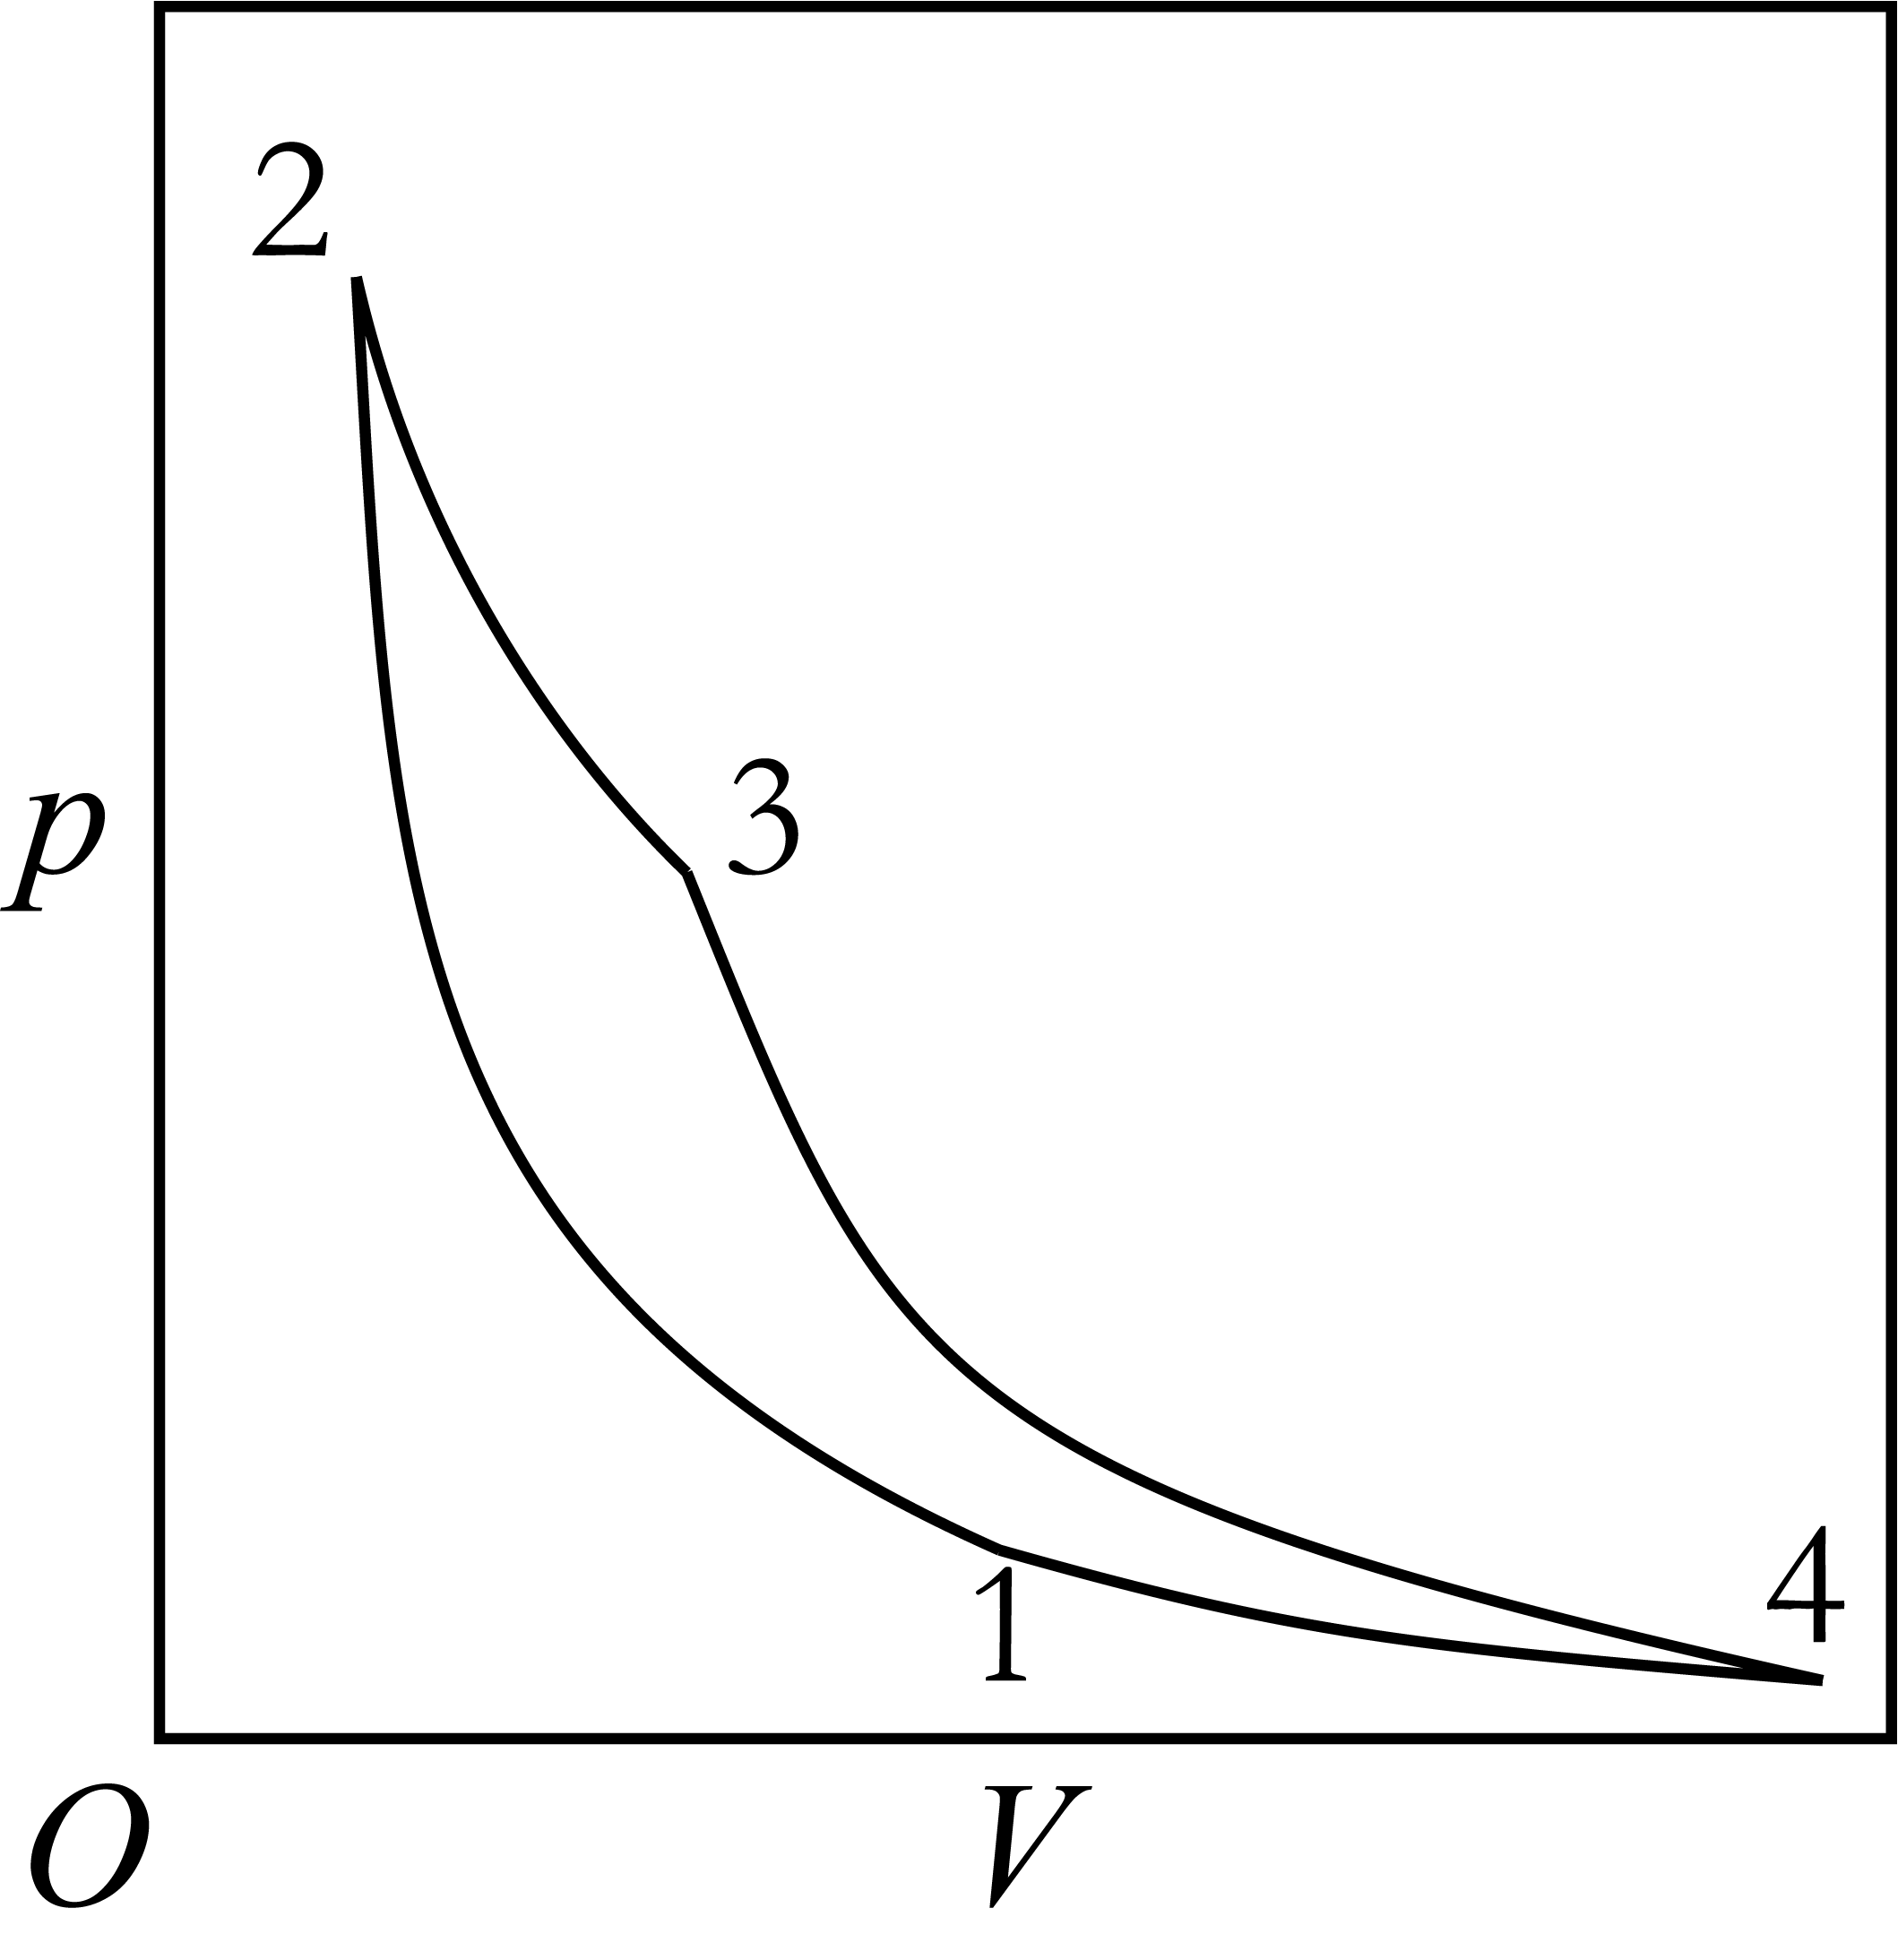
\includegraphics[width=5cm]{image/5-2-10.png}
\caption{Carnot cycle}
\end{wrapfigure}
整个循环由两条绝热线与两条等温线围成.\,过程如下:

\begin{enumerate}[i]
	\item 1-2:\,绝热压缩
	\item 2-3:\,等温吸热
	\item 3-4:\,绝热膨胀
	\item 4-1:\,等温放热
\end{enumerate}

高温热源的温度为$T_{\rm H}$,\,低温冷库的温度为$T_{\rm L}$.\,那么可以计算出卡诺热机的效率为:
\[\eta=1-\frac{T_{\rm L}}{T_{\rm H}}\]


\section{理想气体的熵}

理想气体的准静态过程是这一章内我们关心的问题.\,如何判断一个微元准静态过程中理想气体吸热还是放热?\,具体来说,\,我们关心在$(T,\,V)$点沿着$(\ud T,\,\ud V)$变化方向改变状态所需要吸收的热量微分$\dbar Q$.\,由热一,\,它应为:
\[\dbar Q=\ud U+p\ud V=\nu C_{mV}\ud T+\frac{\nu RT}{V}\ud V\]

这可以进行如下的化简:
\[\dbar Q=\nu C_{mV} T\cdot [\frac{\ud T}{T}+(\gamma-1)\frac{\ud V}{V}]=\nu C_{mV} T\cdot\ud \ln(TV^{\gamma-1})\]

我们定义态函数\ca \emph{熵}(entropy):
\[S_1=\nu C_{mV}\ln(TV^{\gamma-1})\]

那么自然得出:
\[\dbar Q=T\ud S_1\]

这给出了气体吸放热与状态变化之间的联系.\,一个直接的推论就是,\,准静态绝热过程中$TV^{\gamma-1}$是不变的(绝热方程).\,或者说,\,准静态绝热过程可以被称为\emph{等熵过程}(isentropic process).\,而熵作为一个态函数,\,等熵线就是绝热线.

熵在定义时可以相差一个与状态无关的常数(但与摩尔数$\nu$有关,\,目前它不随着状态变化而变化).\,我们为了方便暂时不写这个常数.\,但如果我们一开始以$(p,\,V)$或者$(p,\,T)$作为状态参量.\,那么自然而然写出来的符合$\dbar Q=T\ud S$的熵为:
\[S_2=\nu C_{mV}\ln(pV^\gamma)\quad ;\quad S_3=\nu C_{mV}\ln\frac{T^\gamma}{p^{\gamma-1}}\]

它们都相差一个过程不变的常数:
\[S=S_3\quad ;\quad S_1=S+\nu R\ln(\nu R)\quad ;\quad S_2=S+\nu C_{mp}\ln(\nu R)\]

我们把$S_3$取为标准的熵.\,原因在于,\,如果我们要讨论摩尔数$\nu$变化的情况时.\,在对数里放两个强度量可以使表达式成为一个广延量\ca 当摩尔数增大到$\lambda$倍而所有强度量不变时,\,熵$S$也增大到$\lambda$倍.\,而其他两个$S$附加的项$\nu R\ln(\nu R)$与$\nu C_{mp}\ln(\nu R)$使得定义失去了这种广延性.

\begin{figure}[H]
\centering
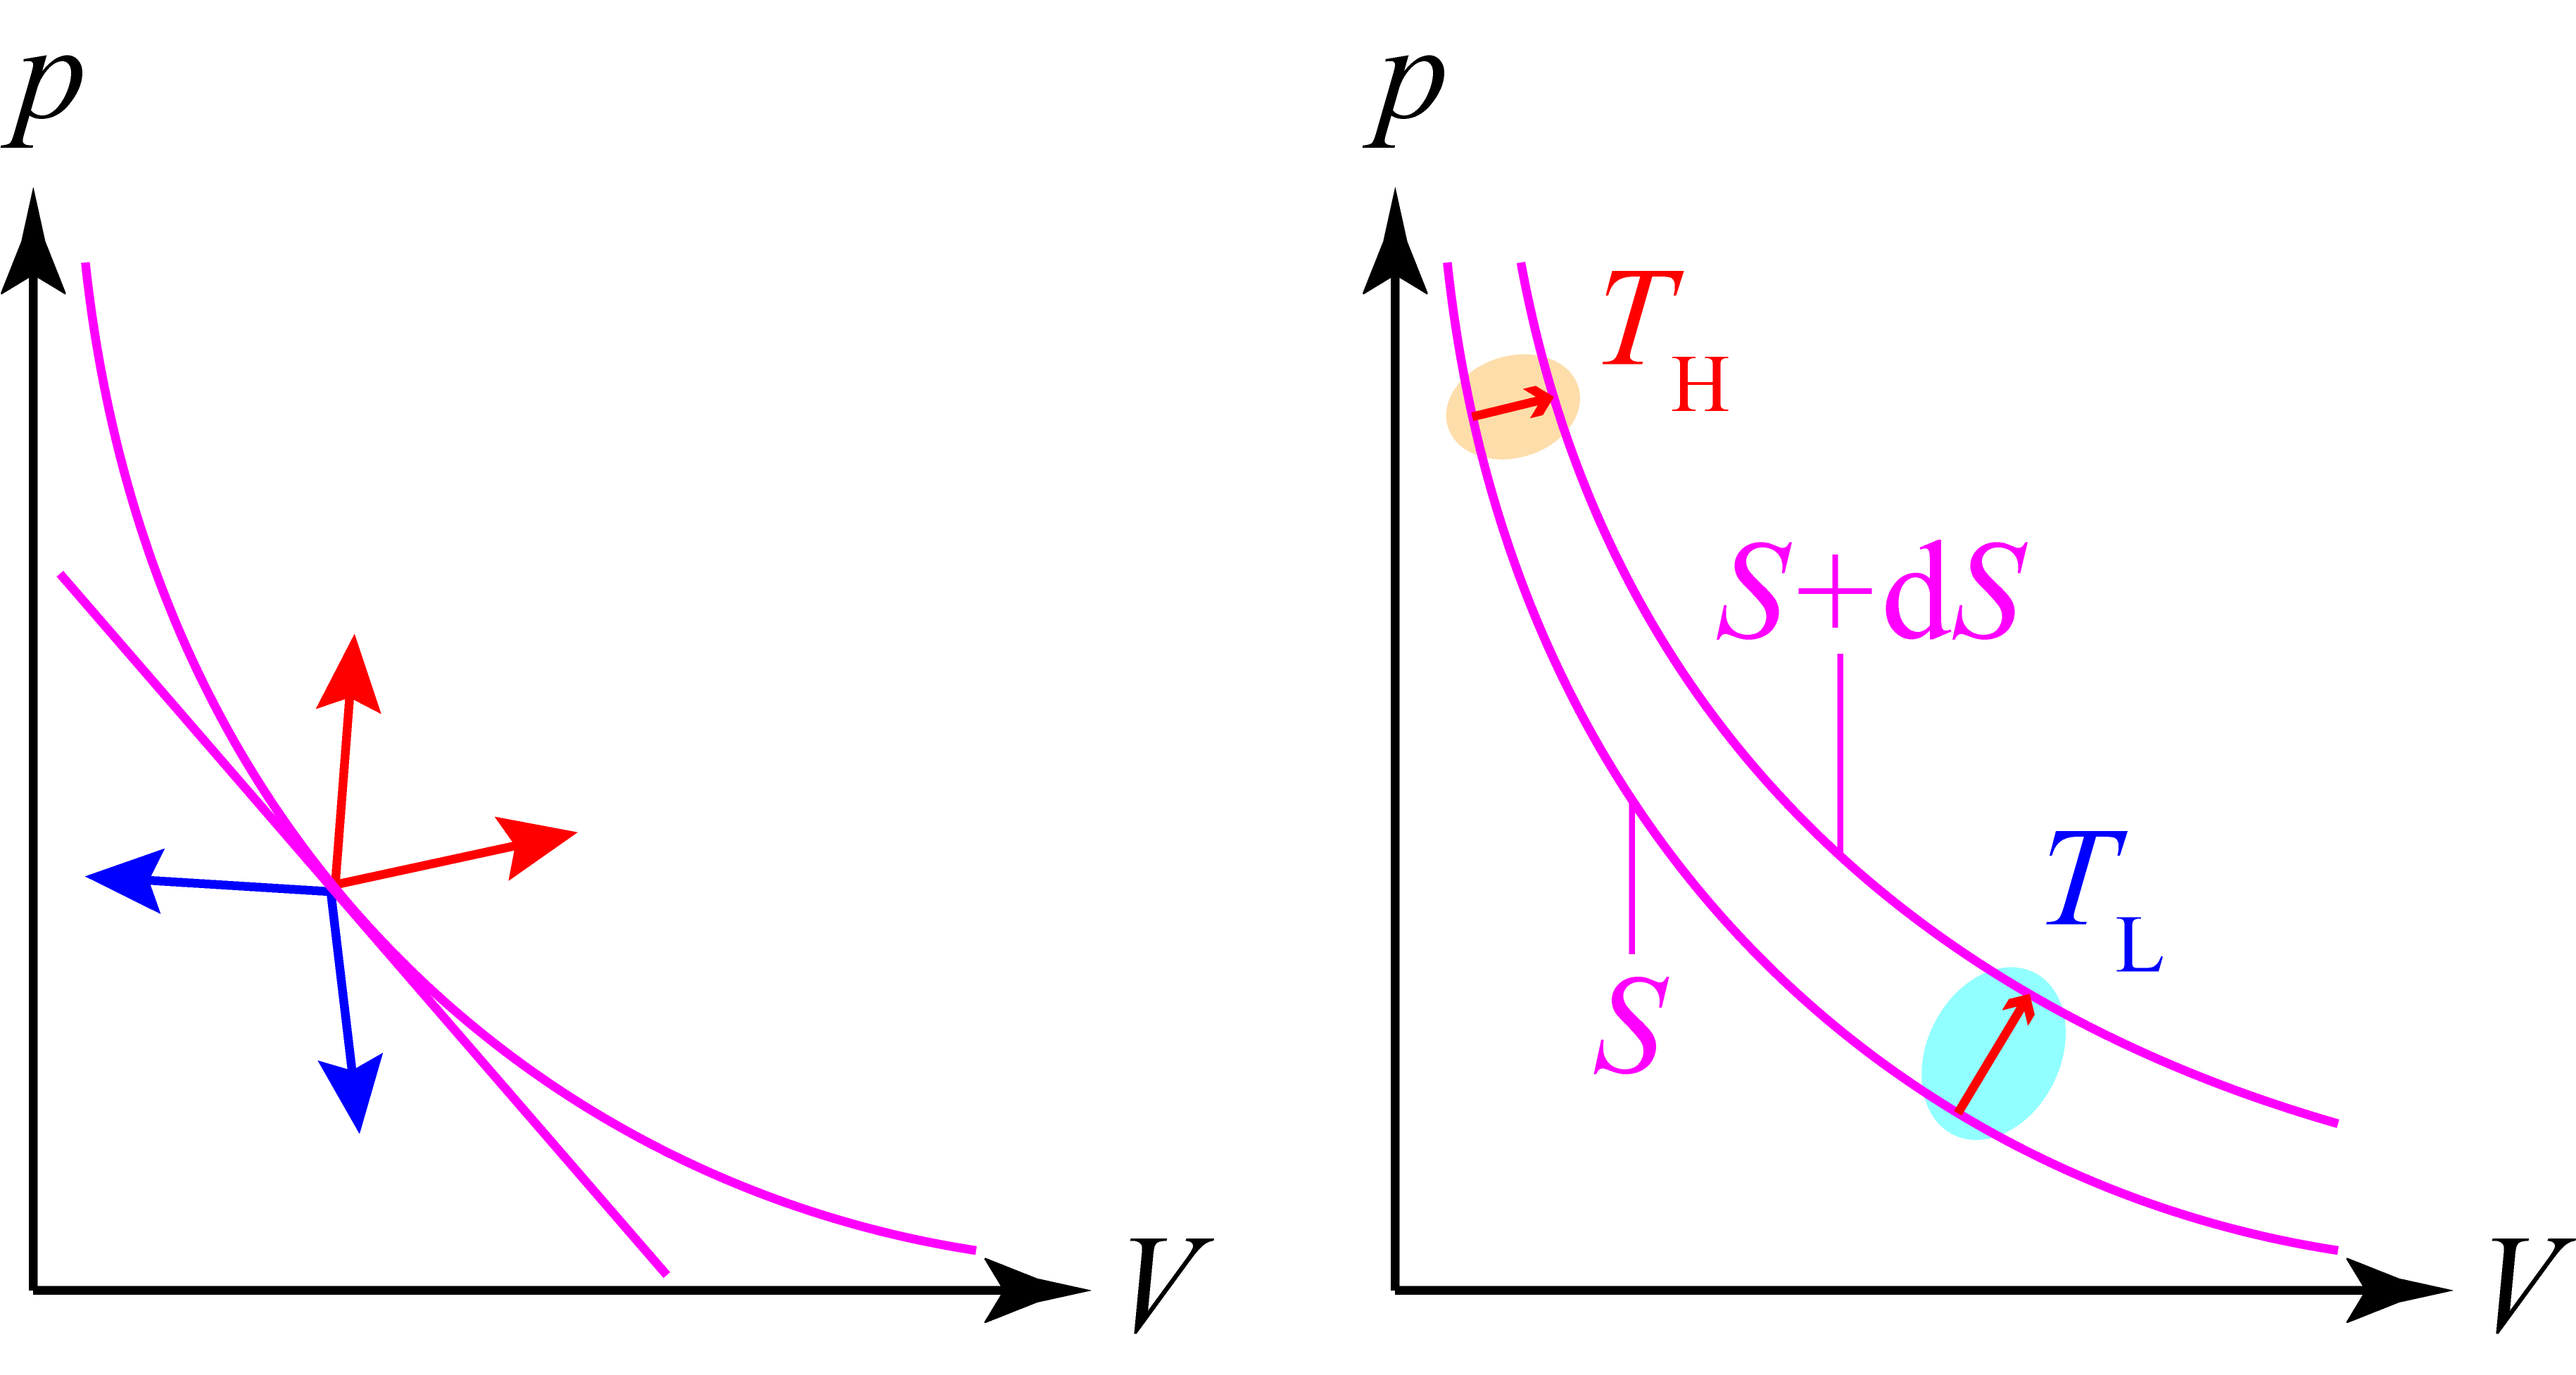
\includegraphics[width=15cm]{image/5-2-11.png}
\caption{左:\,吸放热的元过程方向;\,右:\,两根等熵线间的``热量差''}\label{fig5-2-11}
\end{figure}

我们由此得出这样的结论:\,在一个准静态过程中.\,沿着等熵线以下的方向熵降低(如图\ref{fig5-2-11}中蓝色箭头方向),\,从而要放热.\,而往上走则熵增加,\,要吸热.\,但注意到既使沿着切线方向走熵还是会降低(无论往上还是往下),\,只不过这时候其降低是一个二阶小量而已.\,也就是说如果气体历经$p-V$图上的负斜率直线过程,\,一定是先吸热,\,后放热.\,在中间有一个熵的极值点符合:
\[k=\frac{\ud p}{\ud V}=-\gamma\frac{p}{V}\]

我们画出两条相隔很近的等熵线(差$\ud S$).\,注意到两条线之间的``热量差''这个概念本身不够严谨,\,因为热量是过程量不是状态量.\,但由于两条等熵线相隔很近,\,所以从一点出发到另一条绝热线上的点还在这一点附近(微元过程,\,取$\Delta S\rightarrow 0$的极限).\,所以可以认为温度近似不变.\,尽管这样,\,吸热仍然与过程发生的平均温度$T$有关:
\[Q_{\rm H}=T_{\rm H}\ud S\quad;\quad Q_{\rm L}=T_{\rm L}\ud S\]

\begin{figure}[H]
\centering
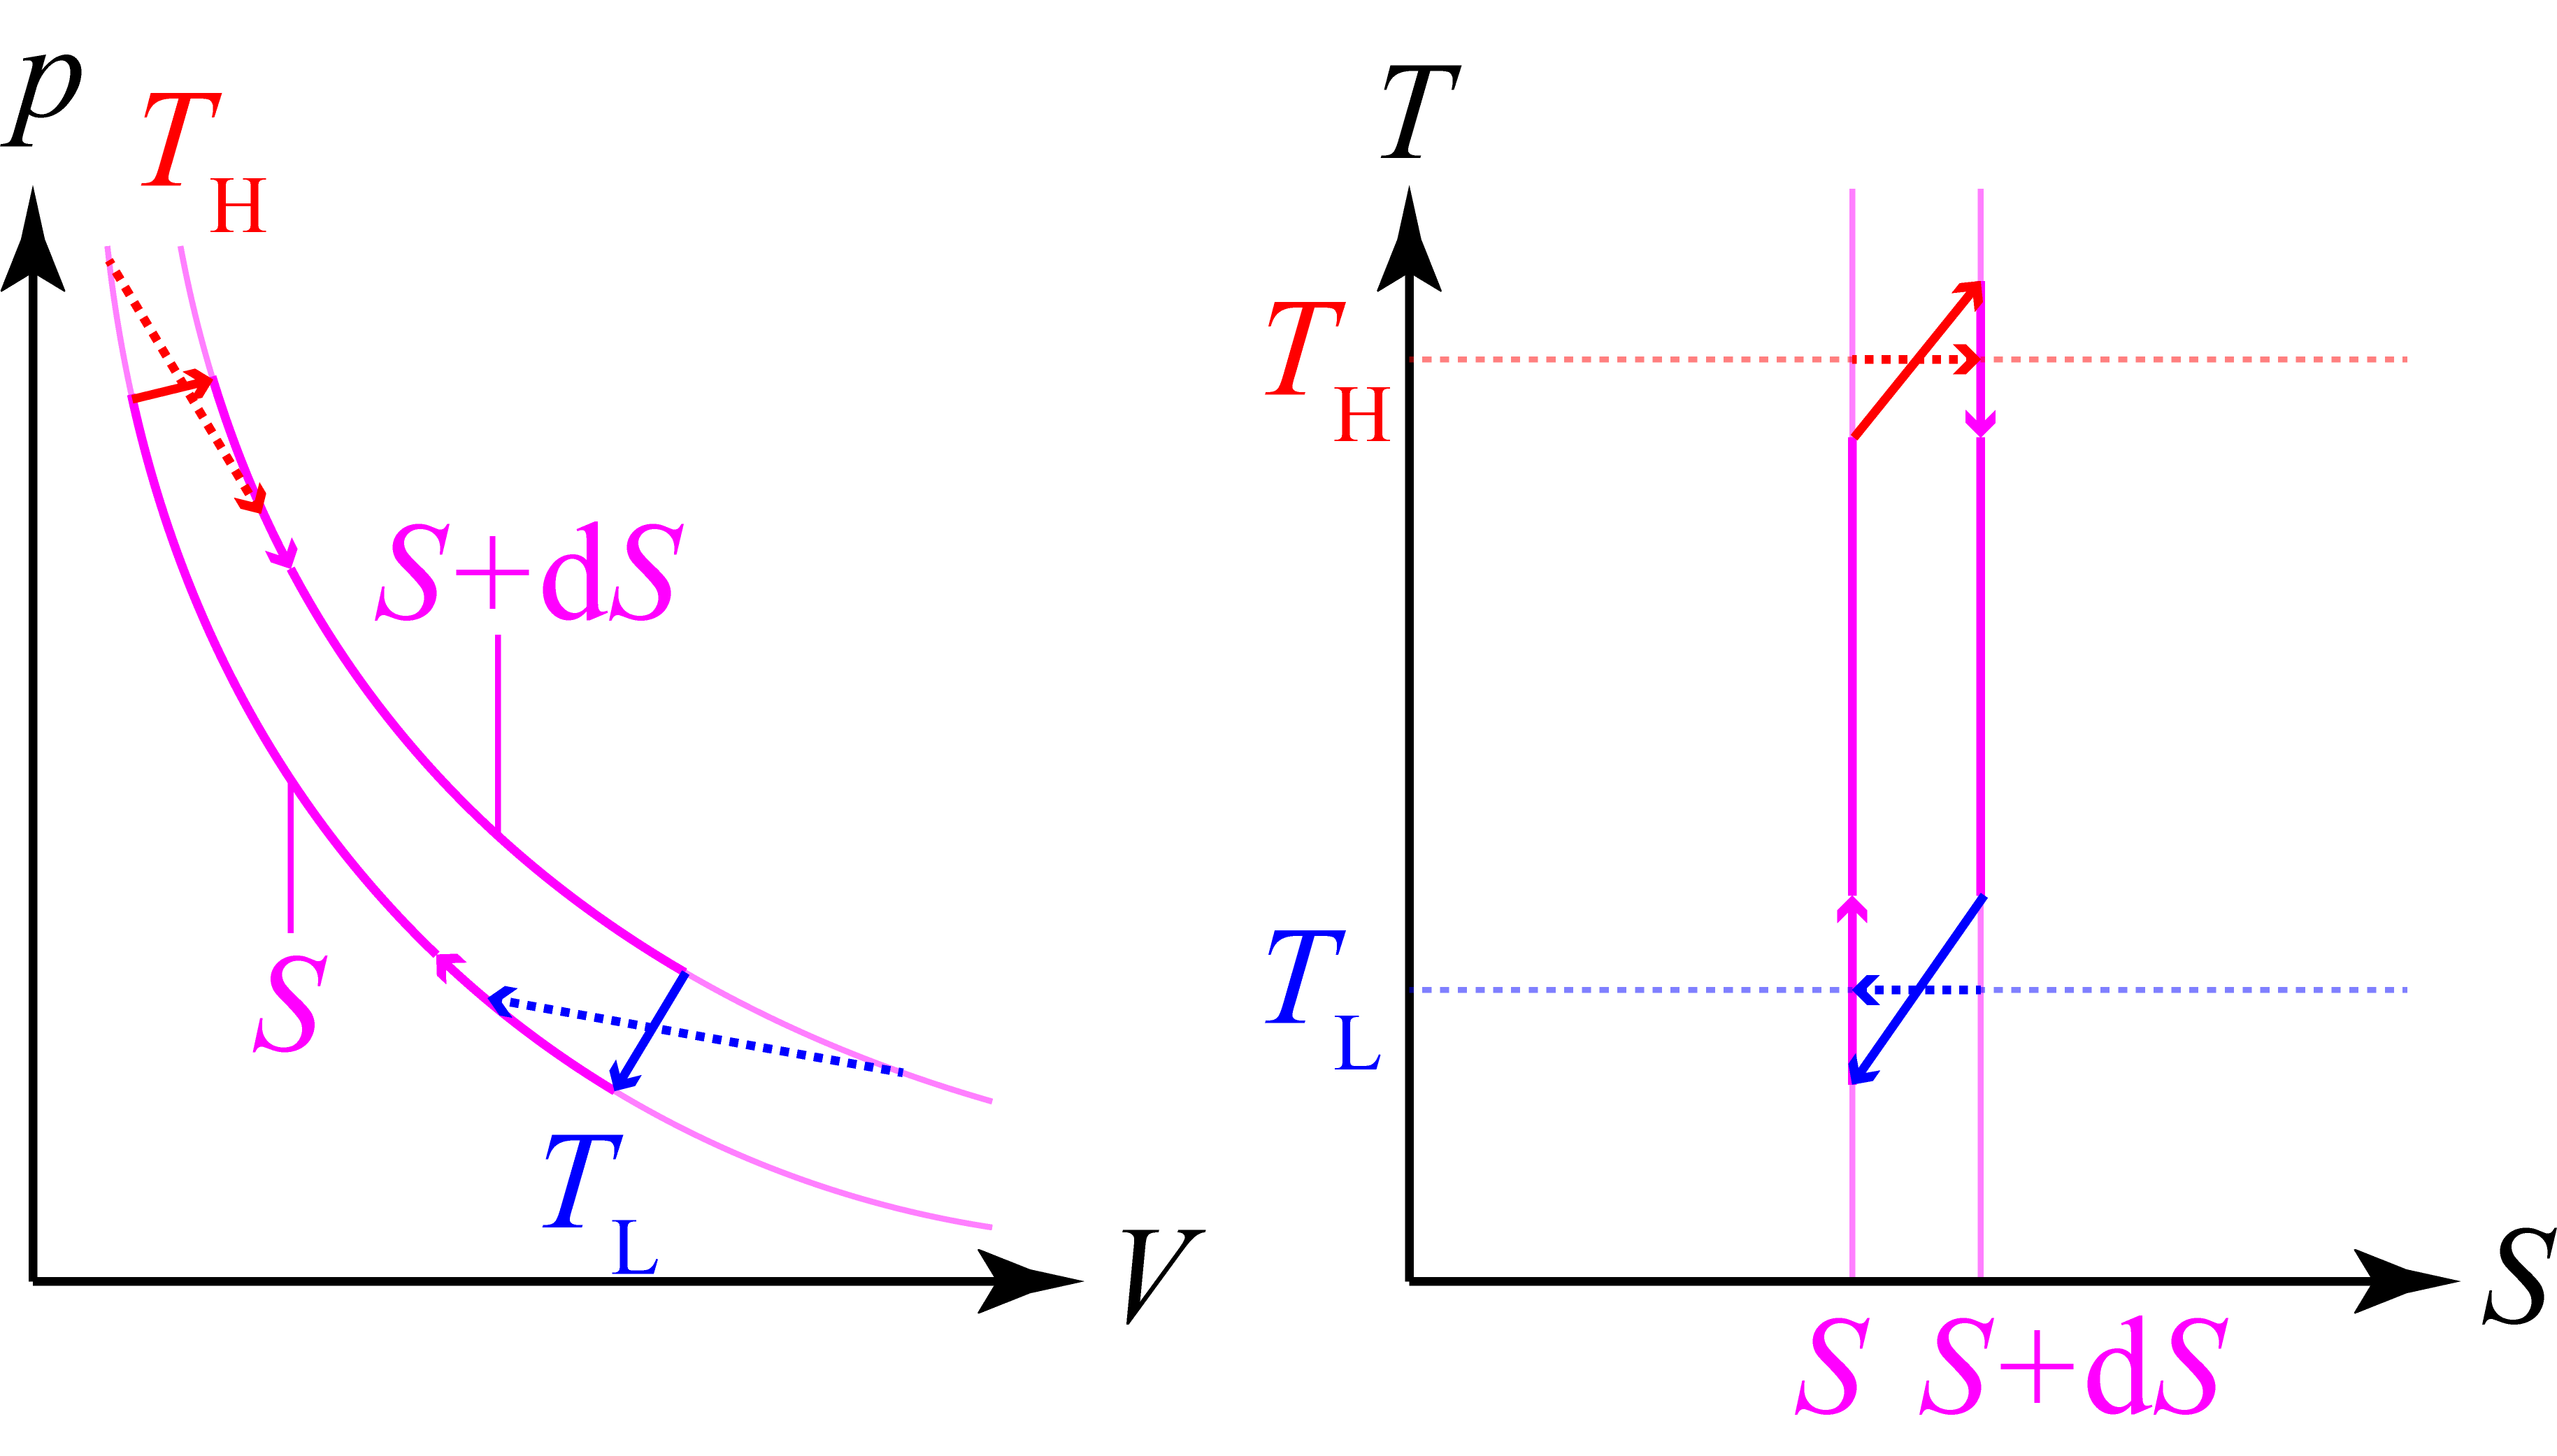
\includegraphics[width=15cm]{image/5-2-12.png}
\caption{示功图与示热图}\label{fig5-2-12}
\end{figure}

由于$S$是态函数,\,我们也可以选取$(T,\,S)$来作为体系的状态参量.\,而做$T-S$图表示状态与过程.\,此时等温线实际上就是水平线,\,而绝热线就是竖直线.\,而其包围的面积实际上就是整个过程所吸收的热量:
\[Q=\oint T\ud S\]

而由于热一,\,它一定等于$p-V$图中的面积,\,它表示对外做功:
\[W=\oint p\ud V\]

正是由于这个直观的关系,\,热力学理论分析时我们经常对照两个图像.\,分别叫做\emph{示功图}(work indicator diagram)与\emph{示热图}(heat indicator diagram).

还有两点值得讨论:

第一,\,以上讨论仅仅限于理想气体的准静态过程.\,我们发现对于理想气体,\,如果采用理想气体温标(即分子内能恰正比于温度),\,恰好可以引入独特的态函数熵来计算其吸热.\,然而,\,对于非准静态过程初末态之间的联系我们还一无所知,\,仅仅知道热一总是成立的.

第二,\,对于其他体系是否有$\dbar Q=T\ud S$?,\,这看上去似乎不显然.\,首先我们知道热力学第零定律定义了温度是某种热平衡的系统共同具有的属性,\,但我们一直使用的温度似乎是根据理想气体的分子平均动能定义出来的(理想气体温标):


这样,\,直接把这个温度用于其他体系似乎不太可能会得出相似的结论,\,而另外定义新的温标又会造成物理规律的不统一性.\,温度也就失去了作为了互为热平衡态共同参数的性质.\,然而,\,需要知道上式不是无来由的,\,它来源于麦克斯韦分布律\ca 微观体系的经典动力学与统计规律的共同结果,\,在这一点上其实温度的定义是普适的,\,它都反应了各个自由度上热运动的剧烈程度.\,所以实际上存在普适的热力学温标,\,而同样的也将存在对应的普适的态函数熵.\,它们都由大量微观粒子的统计规律给出.\,然而十分神奇的一点是,\,普适的温度与熵的存在性在历史上和逻辑上的确是可以由简单的公理得出的热力学第二定律的体系.\,这正是下一节我们要说明的.\,而要深刻了解温度与熵的微观本质需要深入了解统计力学方法,\,我们在下一章将给出相关的论述.
\[T=\frac{2\overline{\varepsilon_k}}{3k}\]


\section{热力学第二定律}

费曼说过,\,所有自然现象的最自然特征莫过于它们明显的不可逆性.\,大量微观粒子构成的宏观热力学体系在种种现象上体现出不可逆的特性,\,即\emph{热力学时间箭头}(time arrow of thermodynamics).\,如果令时间反演,\,系统的各状态逆序发生,\,外界对其做功变为对外做功,\,向外界放热变为从外界吸热.\,那么很多现象都给出了从未被观察到的结果:\,混合均匀地两钟气体自发地分开,\,低温冷库向高温热源自发放热,\,热能单一地转化为机械能等等.\,无耗散的准静态过程是理想的\emph{可逆过程}(reversible process),\,仅有系统内部处处达到细致平衡,\,在与外界平衡的状态下统一地改变其状态才能将其过程反演而符合物理规律.\,而广泛存在的\emph{不可逆过程}(reversible process),\,一方面在于过程反演的不实际性,\,还在于如果我们把系统和外界各部分视为一整个孤立的体系,\,那么发生的不可逆过程无法通过任何可能的过程回到初始状态.\,在发生不可逆过程的时候,\,体系的某些特征沿着一个方向被永久而不可恢复的改变了,\,衡量这个特征的物理量就是熵,\,而这种断言就是热力学第二定律.\,它回答了热一所不能回答的问题,\,给出了热力学过程发生的方向性与限度.\,对于这些问题的讨论是热二的特色.

热力学第二定律在逻辑体系上承接热力学第零,\,第一定律,\,我们现在取消前面已经有良好定义的理想气体与针对它的温标的概念.\,而热机模型与其效率只取决于吸放热仍然有良好的定义:
\[\eta=1-\frac{Q_{\rm L}}{Q_{\rm H}}\]

\begin{figure}[H]
\centering
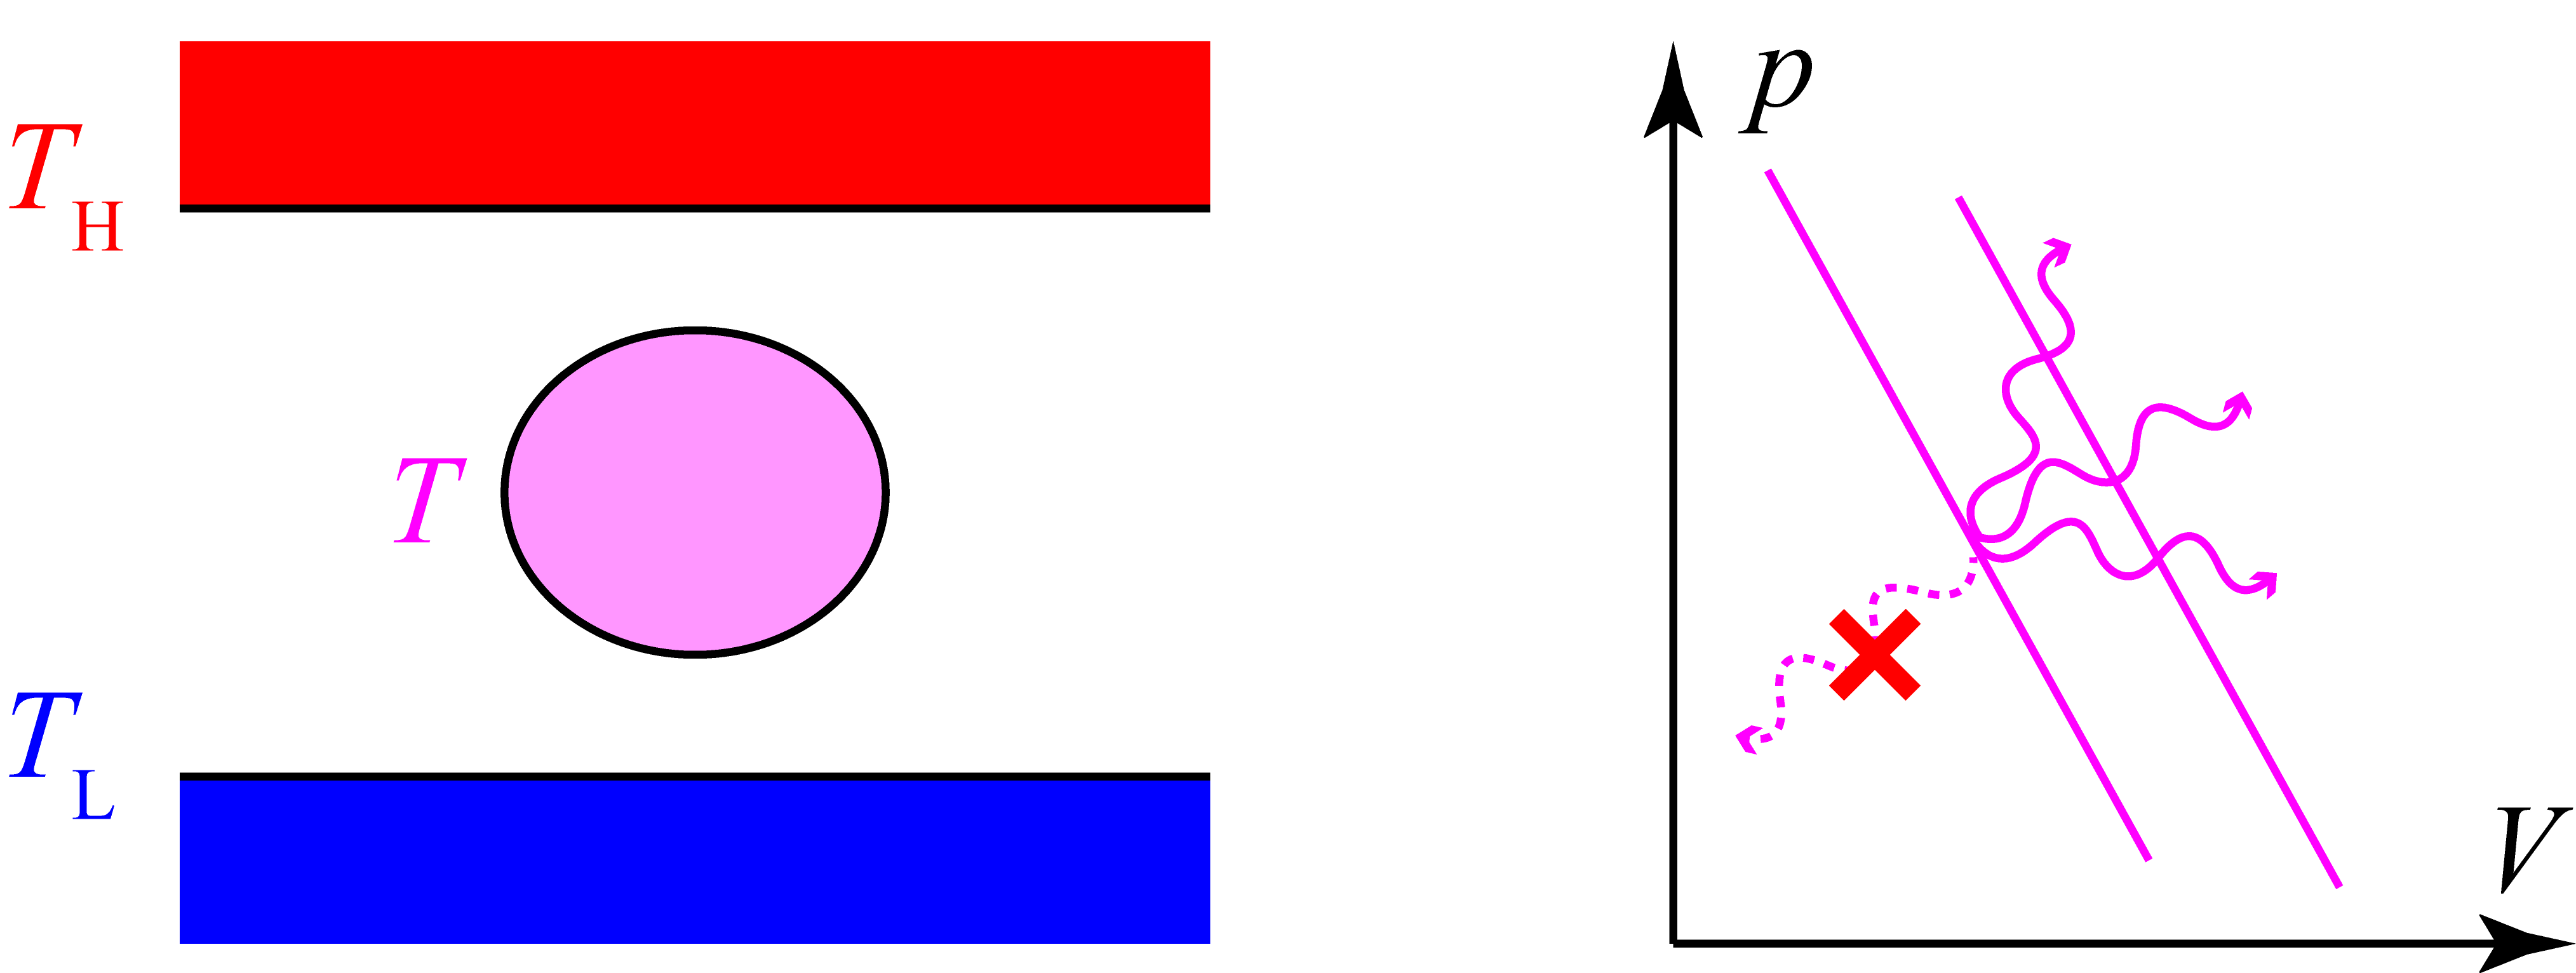
\includegraphics[width=15cm]{image/5-2-13.png}
\caption{熵增原理}\label{fig5-2-13}
\end{figure}
我们讨论一个$p-V$系统作为工作物质在两个恒温热源(冷库在此被称为低温热源)之间的工作,\,各个温度暂时只是一个记号,\,其值暂不确定.\,为了统一起见,\,我们研究系统与外界的功热交换时规定$\ud U=\dbar W+\dbar Q$,\,即以从外界吸热和外界对其做功为正.\,首先,\,我们孤立那个$p-V$系统,\,让它做绝热过程而只能与外界有功的交换.\,那么准静态的绝热过程\footnote{它具有极其独特的含义,\,参见之后第五章的讨论.}将给出系列绝热线,\,它们彼此绝不可以相交,\,否则在一点处将存在多个绝热的方向.\,图中为了简化而近似画成了平行直线(这在微元的循环过程中\ca 微小吸放热,\,微小温差\ca 是合理的处理方法).\,现在考虑一个非准静态的绝热过程.\,如果是绝热压缩,\,那么外界给予气体的压强应该大于系统的平均压强,\,这样造成的不平衡才可以使得系统自发收缩.\,如果是绝热膨胀,\,同理,\,外界给予气体的压强应该小于系统的平均压强.\,不管怎样,\,都有:
\[\dbar W \geq -p\ud V\]

这样造成的结果是系统的状态只能往绝热线的一侧走,\,类似于热力学第零定律,\,对于这个特定体系,\,我们暂时可以把这些可以通过准静态绝热过程相互连接的状态称为具有共同的熵.\,而更高的绝热线代表更高的熵,\,以上观点给出了\emph{熵增原理}(principle of entropy increase):

\begin{center}
\hei 熵增原理:\,孤立系统的熵只增不减,\,$\Delta S \geq 0$
\end{center}

这一点的意义不仅仅在于末态到达另一条绝热线上以后仍然孤立地自发回到初始状态,\,还意味着既使借助外界\ca 两个恒温热源,\,可能出现的其他辅助工作物质的帮助,\,也无法在不改变其他物体的状态(两个热源净吸放热为零,\,其他工作物质初末状态复原)的条件下回到初始状态,\,原来的功也被补偿.\,这构成热力学第二定律的一种表述,\,它在热力学体系里是公理,\,代表了自然界的某种规律.

\begin{figure}[H]
\centering
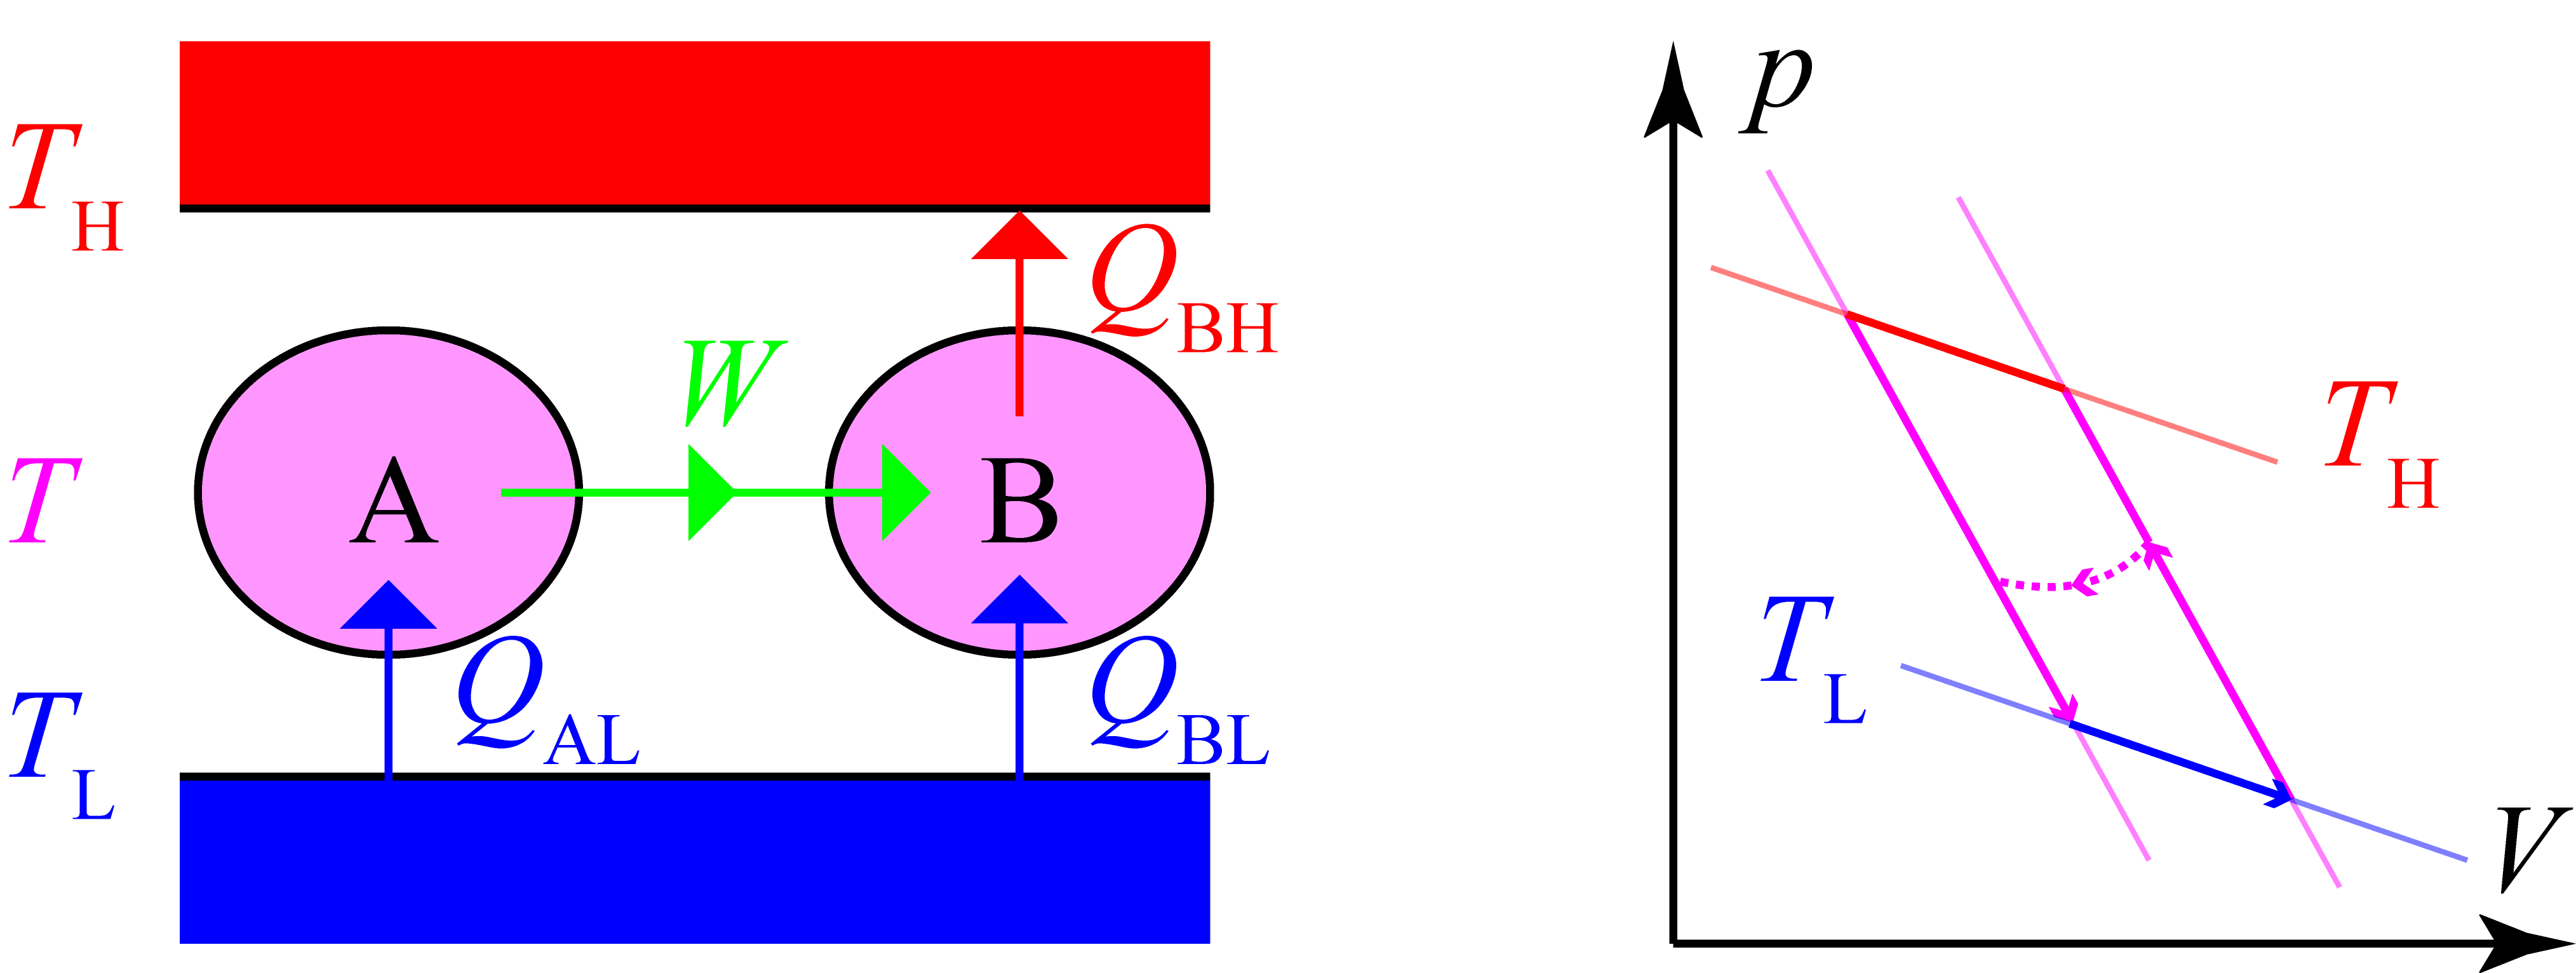
\includegraphics[width=15cm]{image/5-2-14.png}
\caption{三种不可逆过程的联系}\label{fig5-2-14}
\end{figure}

质疑这一点会引发什么结果?\,如果在某个任意中间温度$T,\,T_{\rm L}<T<T_{\rm H}$下可以通过某个过程让较高绝热线上的状态回到相距很近的较低绝热线上的状态.\,那么我们将它与两条绝热线和在低温热源上吸热膨胀的过程组成一个循环,\,其合效果是从低温热源吸收了热,\,并完全转变为对外界的做功.\,这也是被热力学第二定律禁止的,\,或者说其反过程不可逆:

\begin{center}
\hei 开尔文表述:\,功变热不可逆,\,$W=-Q\geq 0$
\end{center}

表述为文字,\,则为热机不可能在一个循环过程中从单一热源吸热转变为对外做功而不产生其他影响.

继续质疑这一点.\,再构造一个热泵B,\,它接受来自热机A的功而从低温热源向高温热源泵热,\,其总结果是,\,低温热源向高温热源传了热,\,其他体系状态历经一个循环回到初态.\,同样的,\,它被热力学第二定律禁止:

\begin{center}
\hei 克劳修斯表述:\,温差传热不可逆,\,$Q_{\rm H}=-Q_{\rm L}\geq 0$
\end{center}

可见热力学第二定律的不同表述之间都是相互联系的.\,实际上如果把两个热源和工作物质视为整体,\,那么其实后两个表述就是整个体系的熵增原理,\,此时,\,整个循环过程来看,\,如果过程中时时,\,处处都是无耗散的准静态过程,\,那么熵应该是不变的,\,过程应该是可逆的,\,这就是卡诺热机模型:\,是高温热源与气体等温时放热$Q_{\rm H}>0$,\,气体与低温热源等温时再放热$|Q_{\rm L}<0|$.\,而气体对外做功为$|W=-Q_{\rm H}-Q_{\rm L}<0|$.\,或者是这个过程的逆过程\ca 卡诺热泵循环.\,对于所有热机,\,热力学第二定律断言:

\begin{center}
\hei 卡诺定理:\,卡诺热机效率最高,\,$\displaystyle \eta=1-\frac{-Q_{\rm L}^\prime}{Q_{\rm H}^\prime}\leq 1-\frac{-Q_{\rm L}}{Q_{\rm H}}$
\end{center}

证明思路是,\,如果有热机效率高于卡诺热机效率,\,意味着输出相同的功时其在两个热源的吸放热可以同时减到比卡诺热机小,\,那么用输出的功给一个对应的卡诺热泵,\,总的结果是低温热源向高温热源放热了,\,由于热力学第二定律,\,这不可以成立.

从而,\,卡诺定理实际上也是热力学第二定律的等价表述.\,这些表述都有一个特点,\,可逆过程对应取等号,\,而不等号发生在不可逆的过程中,\,代表过程的方向性.\,在等号情况下,\,工作于两个恒温热源间的可逆卡诺热机的吸放热比是恒定的,\,这给出了热力学温标的定义:
\[\frac{-Q_{\rm L}}{Q_{\rm H}}=\frac{T_{\rm L}}{T_{\rm H}}\]

只需确定一种特定系统的温度,\,便可以由可逆循环的吸放热比测量任意其他平衡态的温度.\,目前,\,这种特定的系统被取做水的三相共存系统\footnote{2018年预通过的新国际单位制提案指出将可能把联系微观统计规律与宏观测量的常数$k_B$作为基本常数.\,这样确定了温度与能量换算的线性关系,\,从极低温到极高温完全一致.},\,温度定义为$273.16{\rm K}$.\,这就是热力学温标.\,而这也给出了与之共轭的熵的概念:
\[\ud S=\frac{\dbar Q}{T}\]

上式对可逆过程适用.\,对于卡诺循环来说,\,如果着眼点在整个系统,\,那么一个循环下来工作物质的熵是复原的.\,而两个恒温热源的熵变根据上面温度的定义:
\[\Delta S=-\frac{Q_{\rm H}}{T_{\rm H}}-\frac{Q_{\rm L}}{T_{\rm L}}=0\]

可见大的系统初末态在一条等熵线(实际上整个循环中每一个状态之间都彼此等熵,\,因为整个系统做绝热可逆过程)上.\,而如果我们着眼点在气体上,\,而且让气体做一个任意的可逆循环过程,\,一定有:
\[\Delta S=\oint \frac{\dbar Q}{T}=0\]

以上式子为克劳修斯等式(Clausius equality),\,同理对于不可逆过程将给出不等式,\,普遍的,\,我们对一个系统,\,有:
\[\Delta S=S_{\rm final}-S_{\rm initial}\geq \int_{\rm initial}^{\rm final}\frac{\dbar Q}{T}\]

上式也是热力学第二定律的表述,\,它十分强大,\,其他表述都可以简单地从这个表述验证.\,它甚至有十分清晰的图像:\,右边是从外界流向系统的熵流,\,左右的区别在于系统内部不平衡条件下的各种流造成的熵产生,\,详见下一节和本章最后一节的相关讨论.\,对于上式,\,如果不等号左边为零,\,可以理解为功变热的不可逆性:\,右边积分里的$\dbar Q$小于零将使得不等式成立,\,说明在过程中体系更自发的行为是接受外界对其做功,\,而以放热的形式形成能量守恒,\,当然条件是初末态等熵\ca 一般考虑循环过程.\,如果不等式右边为零,\,给出了熵增原理\ca 绝热体系的熵只增不减.



\vspace{1cm}
\section{熵的计算}

\subsection{理想气体的熵}

理想气体温标与热力学温标为何统一?\,一者,\,用理想气体温标定义的温度自动符合卡诺定理:\,卡诺循环效率为热力学定义值$\displaystyle\eta=1-\frac{T_{\rm L}}{T_{\rm H}}$,\,且关键是它能使得下式成为全微分:
\[\ud S=\frac{\dbar Q}{T}=\frac{\ud U+p\ud V}{T}=f(T,\,V)\ud T+g(T,\,V)\ud V\]

如果理想气体温标是$T'=h(T)\cdot T$,\,那么$\displaystyle \frac{\dbar Q}{T'}$不可能再是一个全微分,\,而与热力学第二定律定义的温标不一致.\,

二者,\,热力学第二定律的体系看似复杂而充满精巧的构造,\,实则可以在更深的层次:\,微观动力学规律与统计规律的基础上进行自然的推导.\,此时温度,\,熵,\,热量不仅可以普适而简单地定义,\,而且具有清晰的物理图像,\,我们在第五章统计物理基础中展开说明.

所以,\,理想气体的熵我们可以直接使用第二节的推导,\,不过我们这里写作:
\[S(T,\,V)=\nu C_{mV}\ln T+\nu R \ln V\]
\[S(p,\,V)=\nu C_{mV}\ln p+\nu C_{mp} \ln V\]
\[S(p,\,T)=\nu C_{mp}\ln T-\nu R \ln p\]

以上三个定义不太一样,\,差一些取决于摩尔数$\nu$的常数.\,而且只有最下面一个是广延量.\,一种常见的处理方法是把体积换为摩尔体积:
\[V_m=\frac{V}{\nu}\]

摩尔体积实际上与比体积(单位质量的体积)$v$,\,密度$\rho$,\,粒子数密度$n$有如下正反比关系:
\[\rho=\frac{1}{v}=\frac{\mu}{V_m}=nm\]

这样三个式子都变成了广延量.\,它们还差一些与$\nu$成正比,\,对数里面是$R$的一些广延量.\,这种定义的非唯一性很正常,\,实际过程中产生实际效果的是熵的变化量,\,仅有在极低温下,\,讨论量子体系时才需要讨论熵的绝对数值(热力学第三定律).\,还有一点,\,为了使得对数里的物理量不带单位,\,我们规定$p=p_0,\,v=v_0,\,T=T_0$时的熵为零,\,最后得到统一的熵的公式:
\[S=\nu C_{mV}\ln \frac{T}{T_0}+\nu R \ln \frac{v}{v_0}=\nu C_{mV}\ln \frac{p}{p_0}+\nu C_{mp} \ln \frac{v}{v_0}=\nu C_{mp}\ln \frac{T}{T_0}-\nu R \ln \frac{p}{p_0}\]

熵是广延量,\,我们作此要求.\,说明我们可以将一个均匀的系统按某比例分成若干份,\,熵也会随之分成对应比例的份数.\,甚至,\,我们可以将上面的熵除以总分子数,\,得到每一个分子上的熵的结果:
\[\varsigma=\left( \frac{i}{2}+1 \right)k\ln T-k\ln p \]

乍一看这是荒诞的,\,一个分子具有能量可能还比较好理解,\,但是一个分子为何可以具有温度,\,压强,\,甚至熵的概念?\,这些问题需要等我们之后章节研究了熵的统计学和信息学含义以后才能理解.

\subsection{固定热容固体熵}

理想情况下这种固体是以温度为单参数热力学系统,\,其内能为
\[U=CT\]

而吸热就是$Q=C\Delta T$,\,从而熵:
\[dS=C\frac{\ud T}{T}\]

从而:
\[S=C\ln\frac{T}{T_0}\]

\subsection{大热容恒温热库}

无疑,\,这种情况是上一种情形的大热容极限近似,\,如果温度变化$\Delta T$相对于$T$很小:
\[\Delta S=C\ln\frac{T+\Delta T}{T}\simeq\frac{C\Delta T}{T}=\frac{\Delta U}{T}\simeq\Delta{\frac{U}{T}}\]

即此时等价的定义不会造成区别:
\[S=\frac{U}{T}\]

\subsection{传热熵}

\begin{wrapfigure}[14]{o}[-10pt]{6cm}
\centering
\vspace{-0.5cm}
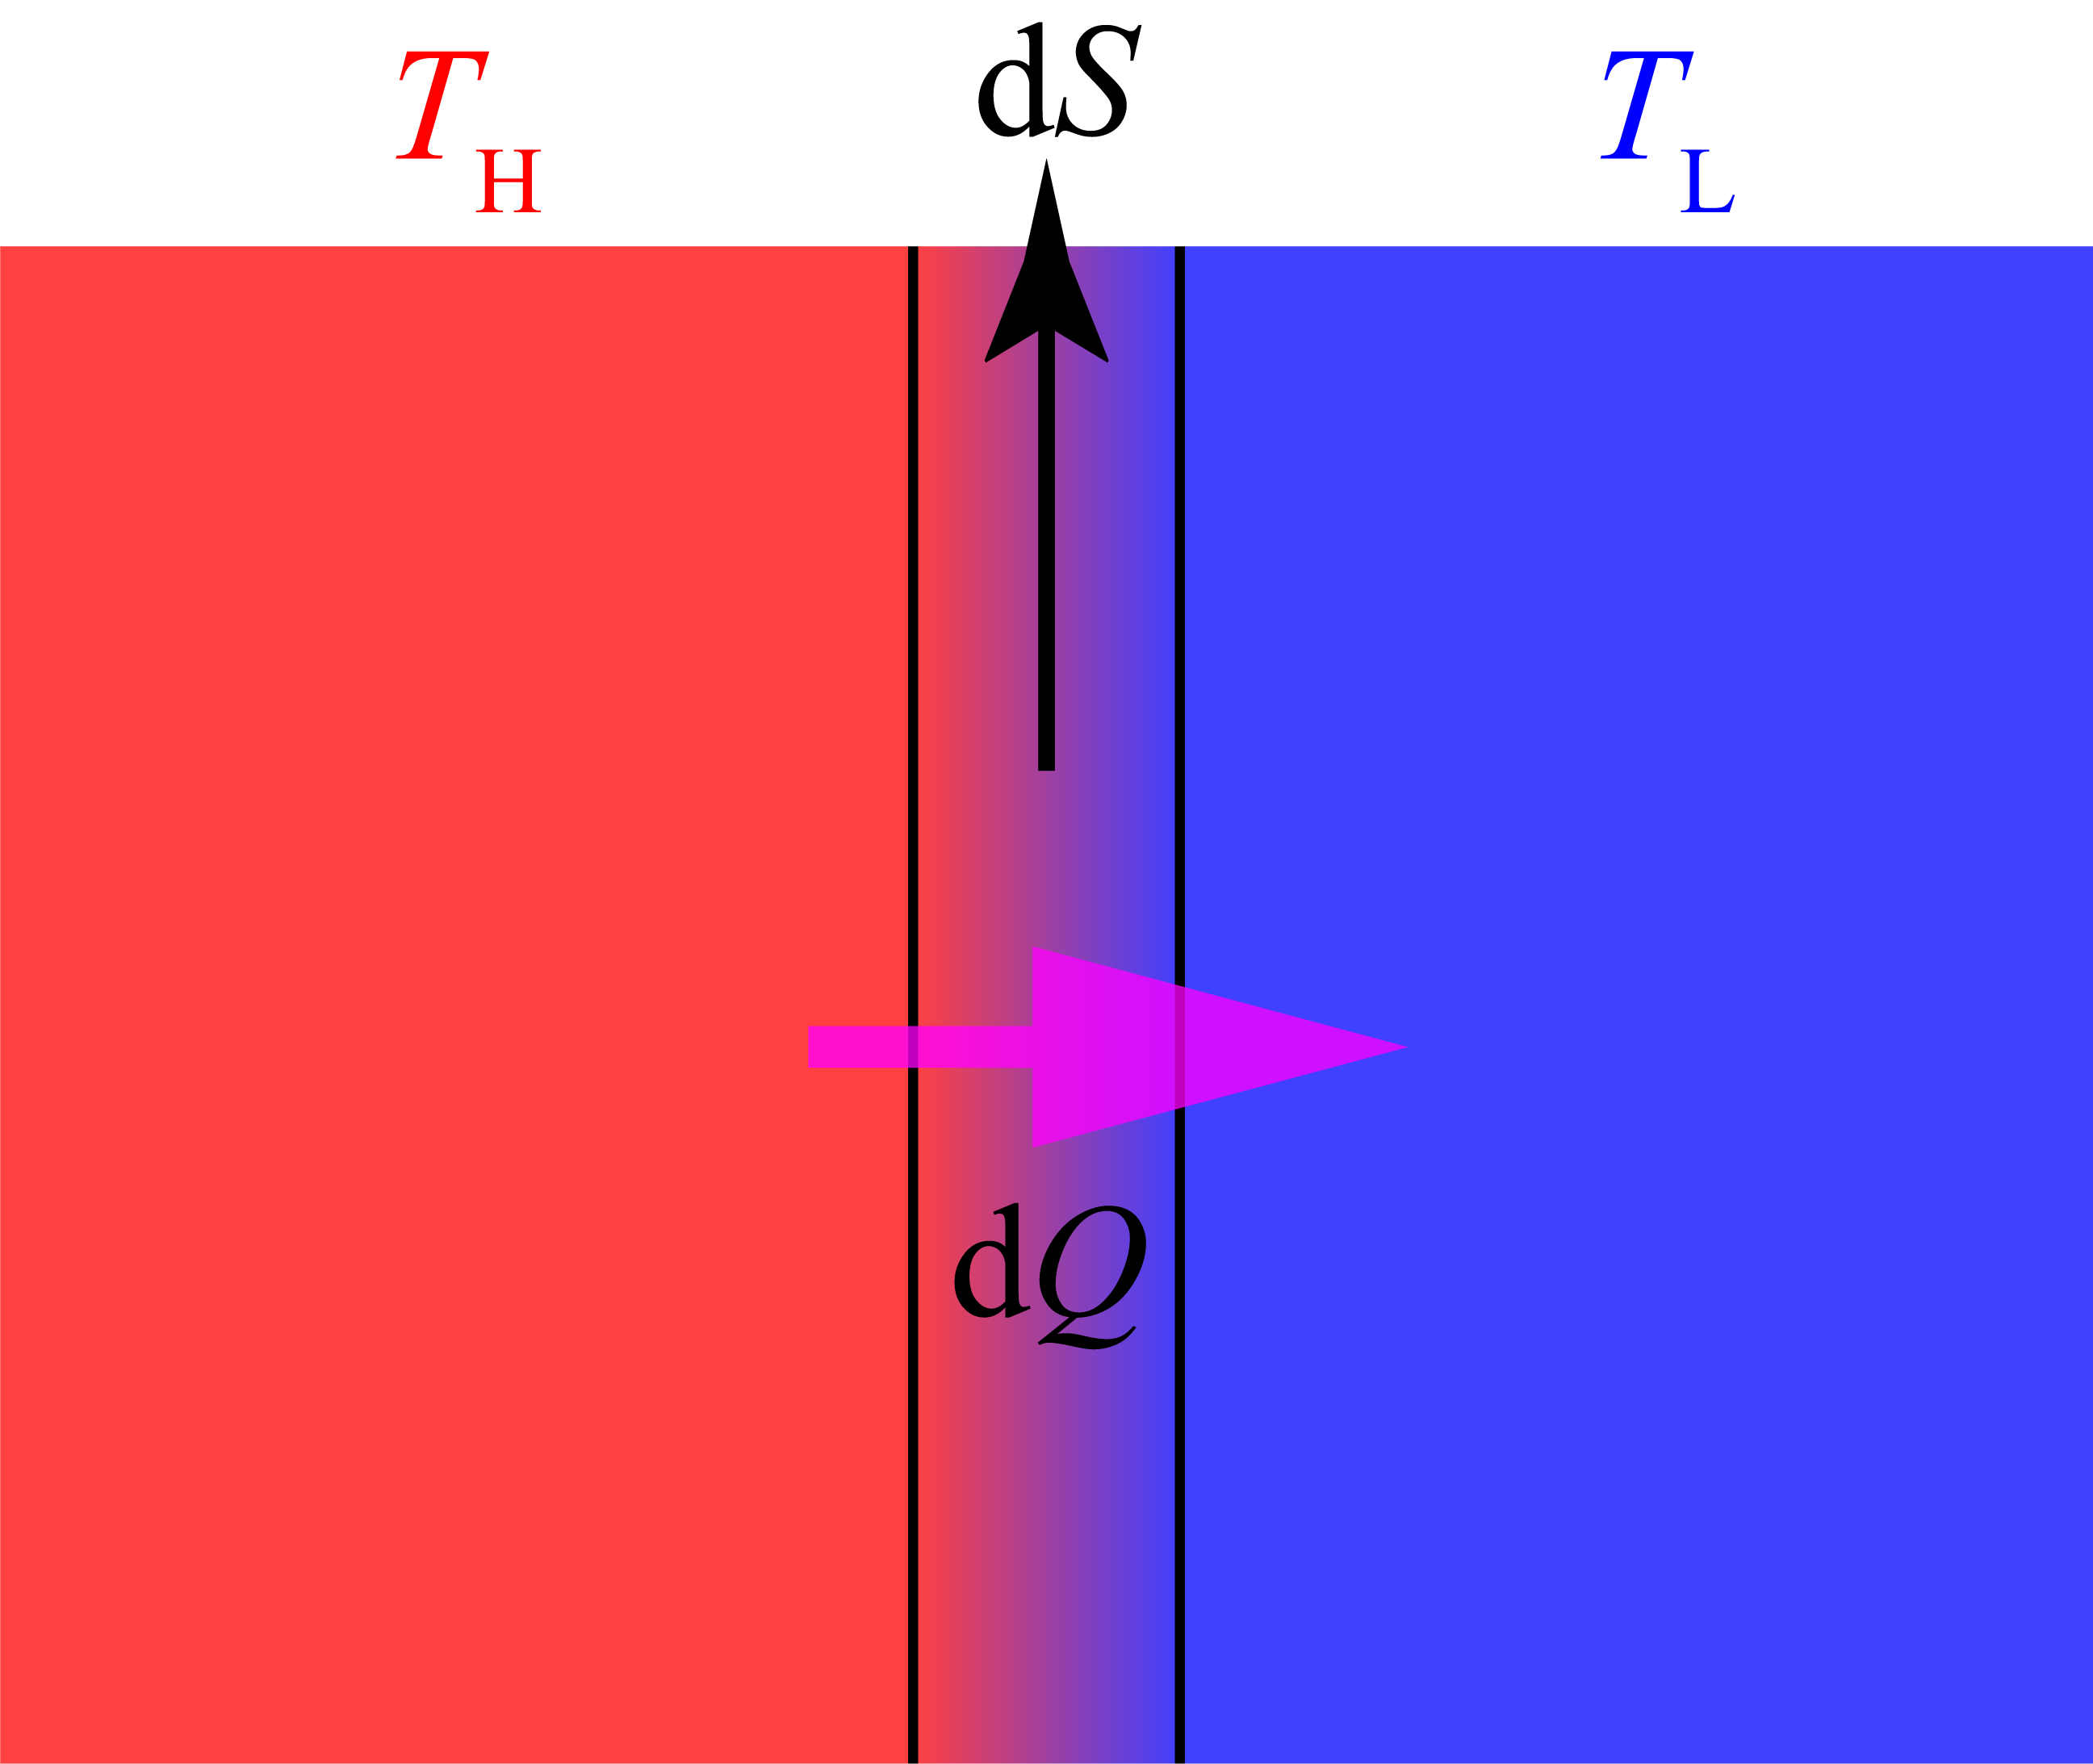
\includegraphics[width=6cm]{image/5-2-15.png}
\caption{传热熵产生}
\end{wrapfigure}
如果高温物体温度$T_{\rm H}$,\,低温物体温度$T_{\rm L}$,\,两者发生一个热接触而有热流$\dbar Q$从高温物体流向低温物体.\,这是一个非准静态过程,\,它不可逆,\,如何分析其熵的呢?\,考虑高温物体放热$\dbar Q$,\,实际上如果它是与一个温度同为$T_{\rm H}$的恒温热库接触而放出这个热量,\,其状态的改变是完全相同的,\,不过这是一个准静态过程,\,可以计算其熵变:
\[\ud S_{\rm H}=-\frac{\dbar Q}{T_{\rm H}}\]

即,\,有$|\ud S_{\rm H}|$的熵从高温物体中流了出来.\,同理,\,流向低温物体的熵为:
\[\ud S_{\rm L}=\frac{\dbar Q}{T_{\rm L}}\]

整个体系熵要增加:
\[\ud S=\dbar Q(\frac{1}{T_{\rm L}}-\frac{1}{T_{\rm H}})> 0\]

上式被称为传热过程中的\emph{熵产生}(entropy production).\,它其实也代表某种微观形式的耗散,\,它发生于高温与低温物体接触时平均起来高温的动能较大的粒子动能被拉低而低温物体动能被拔高的过程中.

\subsection{混合熵}

讨论理想气体的混合,\,而且混合后各种气体分子间亦无任何形式的相互作用.\,命气体的第$i$组分的摩尔分数为$x_i$,\,混合前不同气体处于温度为$T$,\,压强为$p$的平衡,\,不同组分占体积比为:
\[V_1:V_2:\,\cdots\, :V_n=x_1:x_2:\,\cdots\,:x_n\quad ; \quad V_i=x_i V\]

混合后温度仍然是$T$,\,体积倒是共用一个$V$了.\,而不同组分去对$p$进行分压:
\[p_1:p_2:\,\cdots\, :p_n=x_1:x_2:\,\cdots\,:x_n\quad ; \quad p_i=x_i p\]

\begin{wrapfigure}[15]{o}[-10pt]{5cm}
\centering
\vspace{-0.5cm}
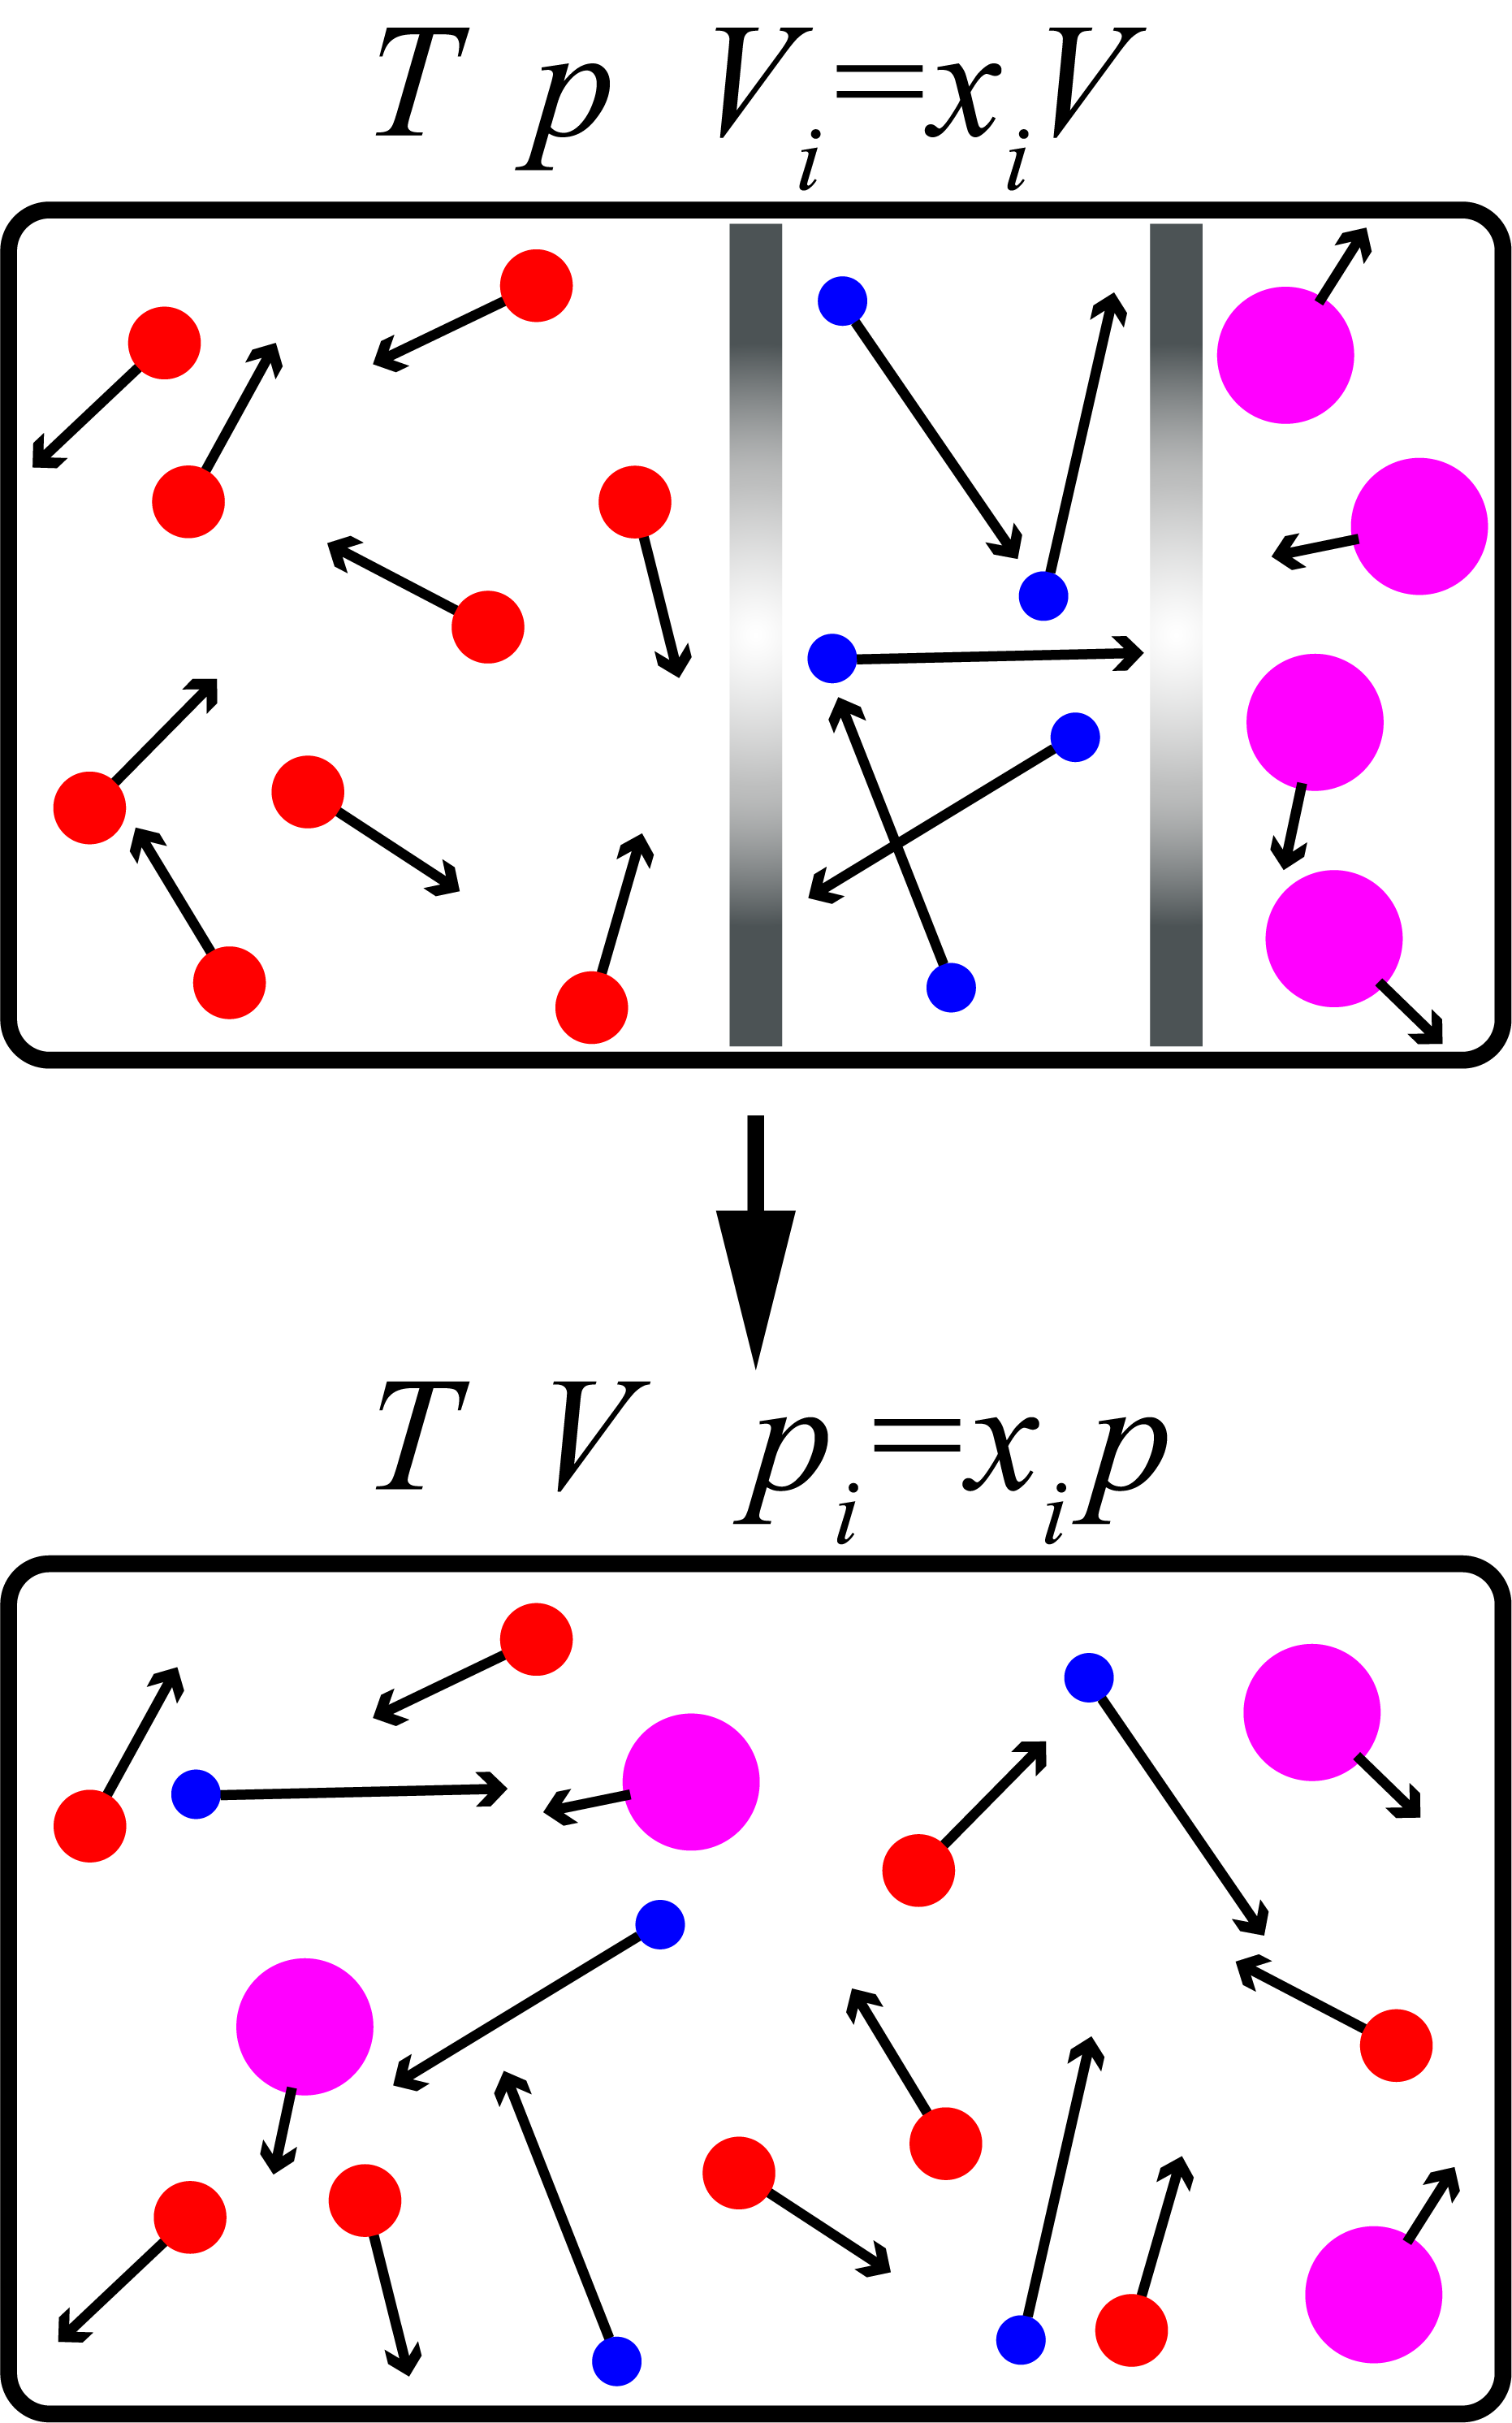
\includegraphics[width=5cm]{image/5-2-16.png}
\caption{混合熵}
\end{wrapfigure}
熵是广延量,\,混合理想气体的熵满足\emph{吉布斯定理}(Gibbs' theorem):\,混合气体的熵等于所有组分的熵的和,\,而每一组分在与其他组分共存的过程中,\,其他组分对这个组分可能的微观状态形式并无影响(分子间无相互作用).\,所以这个组分的熵就等于它单独存在时的熵.\,那么过程前后的熵变其实也就是气体向真空自由膨胀的熵变(因为$T$恰好不变,\,与自有膨胀特征相同),\,这是一个典型的不可逆过程:
\[\Delta S_i=\nu_i R\ln\frac{V}{V_i}=-\nu R x_i\ln x_i\]

故算出\emph{混合熵}(entropy of mixing)为:
\[\Delta S=-\nu R\sum x_i\ln x_i>0\]

我们写出末态混合均匀后熵的表达式,\,注意为了保证其广延性,\,我们采用$p,\,T,\,x_i$这些强度量作为其可以放到$\ln$后面的自变量:
\begin{eqnarray*}
S 	&=&	 \sum S_i \\
	&=&	\sum \nu_i C_{mp}\ln T-\nu_i R\ln p_i \\
	&=&	\nu C_{mp}\ln T-\nu R\ln p-\nu R\sum x_i\ln x_i \\
	&=&	S_0 +\Delta S
\end{eqnarray*}

从中混合熵的概念就十分明显了:\,它代表混合气体与同样条件下的单组分气体的熵$S_0$的区别.\,这很自然地引入了所谓的\emph{吉布斯佯谬}(Gibbs' paradox):\,一是为什么吉布斯定理不适用于单组分气体,\,如果把一缸气体体积分成两份,\,那么熵可以直接相加(广延性),\,但不能把这缸气体的压强(粒子数)分成两份而占据相同的体积,\,除非分成的两份分子有本质的不同.\,二就是多组分与单组分的区别在哪里,\,会造成物理量的差别.

这其实不是奇怪的事.\,我们考虑一缸氢气,\,它的熵应根据$S_0$计算,\,用它计算也符合测量结果.\,而某一天科学家们突然得知,\,原来氢分子${\rm H_2}$分为两种:\,核自旋平行的\emph{正氢}(orthohydrogen)和核自旋反向的\emph{仲氢}(parahydrogen),\,两者占比为$3:1$.\,两种分子仅仅是深入到原子核的性质略有不同,\,对常温下的分子物理化学性质几乎没有影响\footnote{然而低温下影响巨大,\,这与量子效应有关}.\,于是似乎要在熵公式后附加一项混合熵$\displaystyle -\nu R(\frac{1}{4}\ln\frac{1}{4}+\frac{3}{4}\ln\frac{3}{4})\approx 0.56\nu R$.\,这一项如何解释?\,通过第五章的学习我们将知道,\,熵实际上对应着信息的多少.\,在混合氢情况下我们知道了更多的信息:\,每一个氢分子究竟是正氢还是仲氢.\,所以熵增加了.\,但加这一项有必要吗?\,其实是没有必要的,\,因为它作为常数,\,在公式$\dbar Q=T\ud S$中求变化量时不出现,\,从而不会出现在实际可以测量的系统发生的过程中的宏观物理量上.\,然而一涉及到微观构成,\,它就是必要的了,\,如果两种氢之间可以相互转化,\,那么如果整缸氢气都是正氢或是仲氢,\,在一定时间后它将在两种氢之比为$3:1$处平衡,\,这个过程是个不可逆过程.\,这是因为正氢又分为三种可能的自旋态,\,那么把这三个态与仲氢的摩尔分数记做$x_1,\,x_2,\,x_3,\,x_4$,\,有:
\[x_1+x_2+x_3+x_4=1\]
\[\Delta S=-\nu R\ln\sqrt[4]{x_1x_2x_3x_4}\]

由算术几何平均不等式,\,在$\displaystyle x_1=x_2=x_3=x_4=\frac{1}{4}$处熵增取极大值.\,在这个状态往任何一个其他状态熵必然减少而不被热二允许.\,它就是我们要求的平衡态.\,所以两种氢之比为$3:1$,\,同时我们还可以看出之前我们算的熵变还不够严格,\,考虑四种氢时混合熵应为
\[\Delta S=\nu R\ln 4=1.4\nu R\]

值得一提,\,我们上面反过来通过预先在非平衡态都有良好定义的熵的极值来求平衡状态的参数条件的方法称为\emph{最大熵原理}(principle of maximum entropy),\,这种目前看似难以理解的方法亦会在第五章给出详细论述.



\section{热力学函数与其特性}

\subsection{四个热力学函数与四个状态参量}

在本节中我们将把态函数熵$S$视为与$p,\,V,\,T$并列的状态参量.\,由热力学第一定律:
\[\ud U=\dbar Q+\dbar W\]

无论是在准静态或非准静态过程中上式都使用,\,而只有在准静态过程中:
\[\dbar Q= T\ud S\quad;\quad \dbar W=-p\ud V\]

于是:
\[\ud U= T\ud S -p\ud V\]

这个式子又是对准静态和非准静态过程都适用的了,\,因为等式两边都是状态量,\,它们不关心过程的性质.\,这是对符合热力学规律的正确定义的各个物理量之间提出的必然要求,\,被称作\emph{热力学基本方程}(master equation).\.在这里,\,可以理解为如果把内能写作熵$S$和体积$T$的函数,\,它必须满足:
\[\left(\frac{\partial U}{\partial S}\right)_V=T\; ; \; \left(\frac{\partial U}{\partial V}\right)_S=-p\]

由混合偏导数与求导次序无关的性质,\,可以得到:
\[\left(\frac{\partial T}{\partial V}\right)_S=-\left(\frac{\partial p}{\partial S}\right)_V\]

而我们之前定义了焓$H=U+pV$,\,那么相应的有:
\[\ud H= T\ud S +V\ud p\]
\[\left(\frac{\partial H}{\partial S}\right)_p=T\; ; \; \left(\frac{\partial H}{\partial p}\right)_S=V\]
\[\left(\frac{\partial T}{\partial p}\right)_S=\left(\frac{\partial V}{\partial S}\right)_p\]

我们再定义\emph{亥姆霍兹自由能}(Helmholtz's free energy),\,简称\emph{自由能}(free energy)为$F=U-TS$,\,从表达式上看,\,它反映了一种能量最低与熵最高的``抗衡''.\,它的相应结论为:
\[\ud F=- S\ud T -p\ud V\]
\[\left(\frac{\partial F}{\partial T}\right)_V=-S\; ; \; \left(\frac{\partial F}{\partial V}\right)_T=-p\]
\[\left(\frac{\partial S}{\partial V}\right)_T=\left(\frac{\partial p}{\partial T}\right)_V\]

最后还可以定义\emph{自由焓}(free enthalpy),\,它又被叫做\emph{吉布斯自由能}(Gibbs' free energy),\,定义为$G=H-TS=U+pV-TS$,\,相关性质为:
\[\ud G=- S\ud T +V\ud p\]
\[\left(\frac{\partial G}{\partial T}\right)_p=-S\; ; \; \left(\frac{\partial G}{\partial p}\right)_T=V\]
\[\left(\frac{\partial S}{\partial p}\right)_T=-\left(\frac{\partial V}{\partial T}\right)_p\]

\npg{-2cm}
以上四个热力学基本函数的定义自然而然的给出了四个基本关系式,\,称为\emph{麦克斯韦关系}(Maxwell relations):
\[\left(\frac{\partial T}{\partial V}\right)_S=-\left(\frac{\partial p}{\partial S}\right)_V\]
\[\left(\frac{\partial T}{\partial p}\right)_S=\left(\frac{\partial V}{\partial S}\right)_p\]
\[\left(\frac{\partial S}{\partial V}\right)_T=\left(\frac{\partial p}{\partial T}\right)_V\]
\[\left(\frac{\partial S}{\partial p}\right)_T=-\left(\frac{\partial V}{\partial T}\right)_p\]

\begin{wrapfigure}[9]{o}[-10pt]{8cm}
\centering
\vspace{-0.3cm}
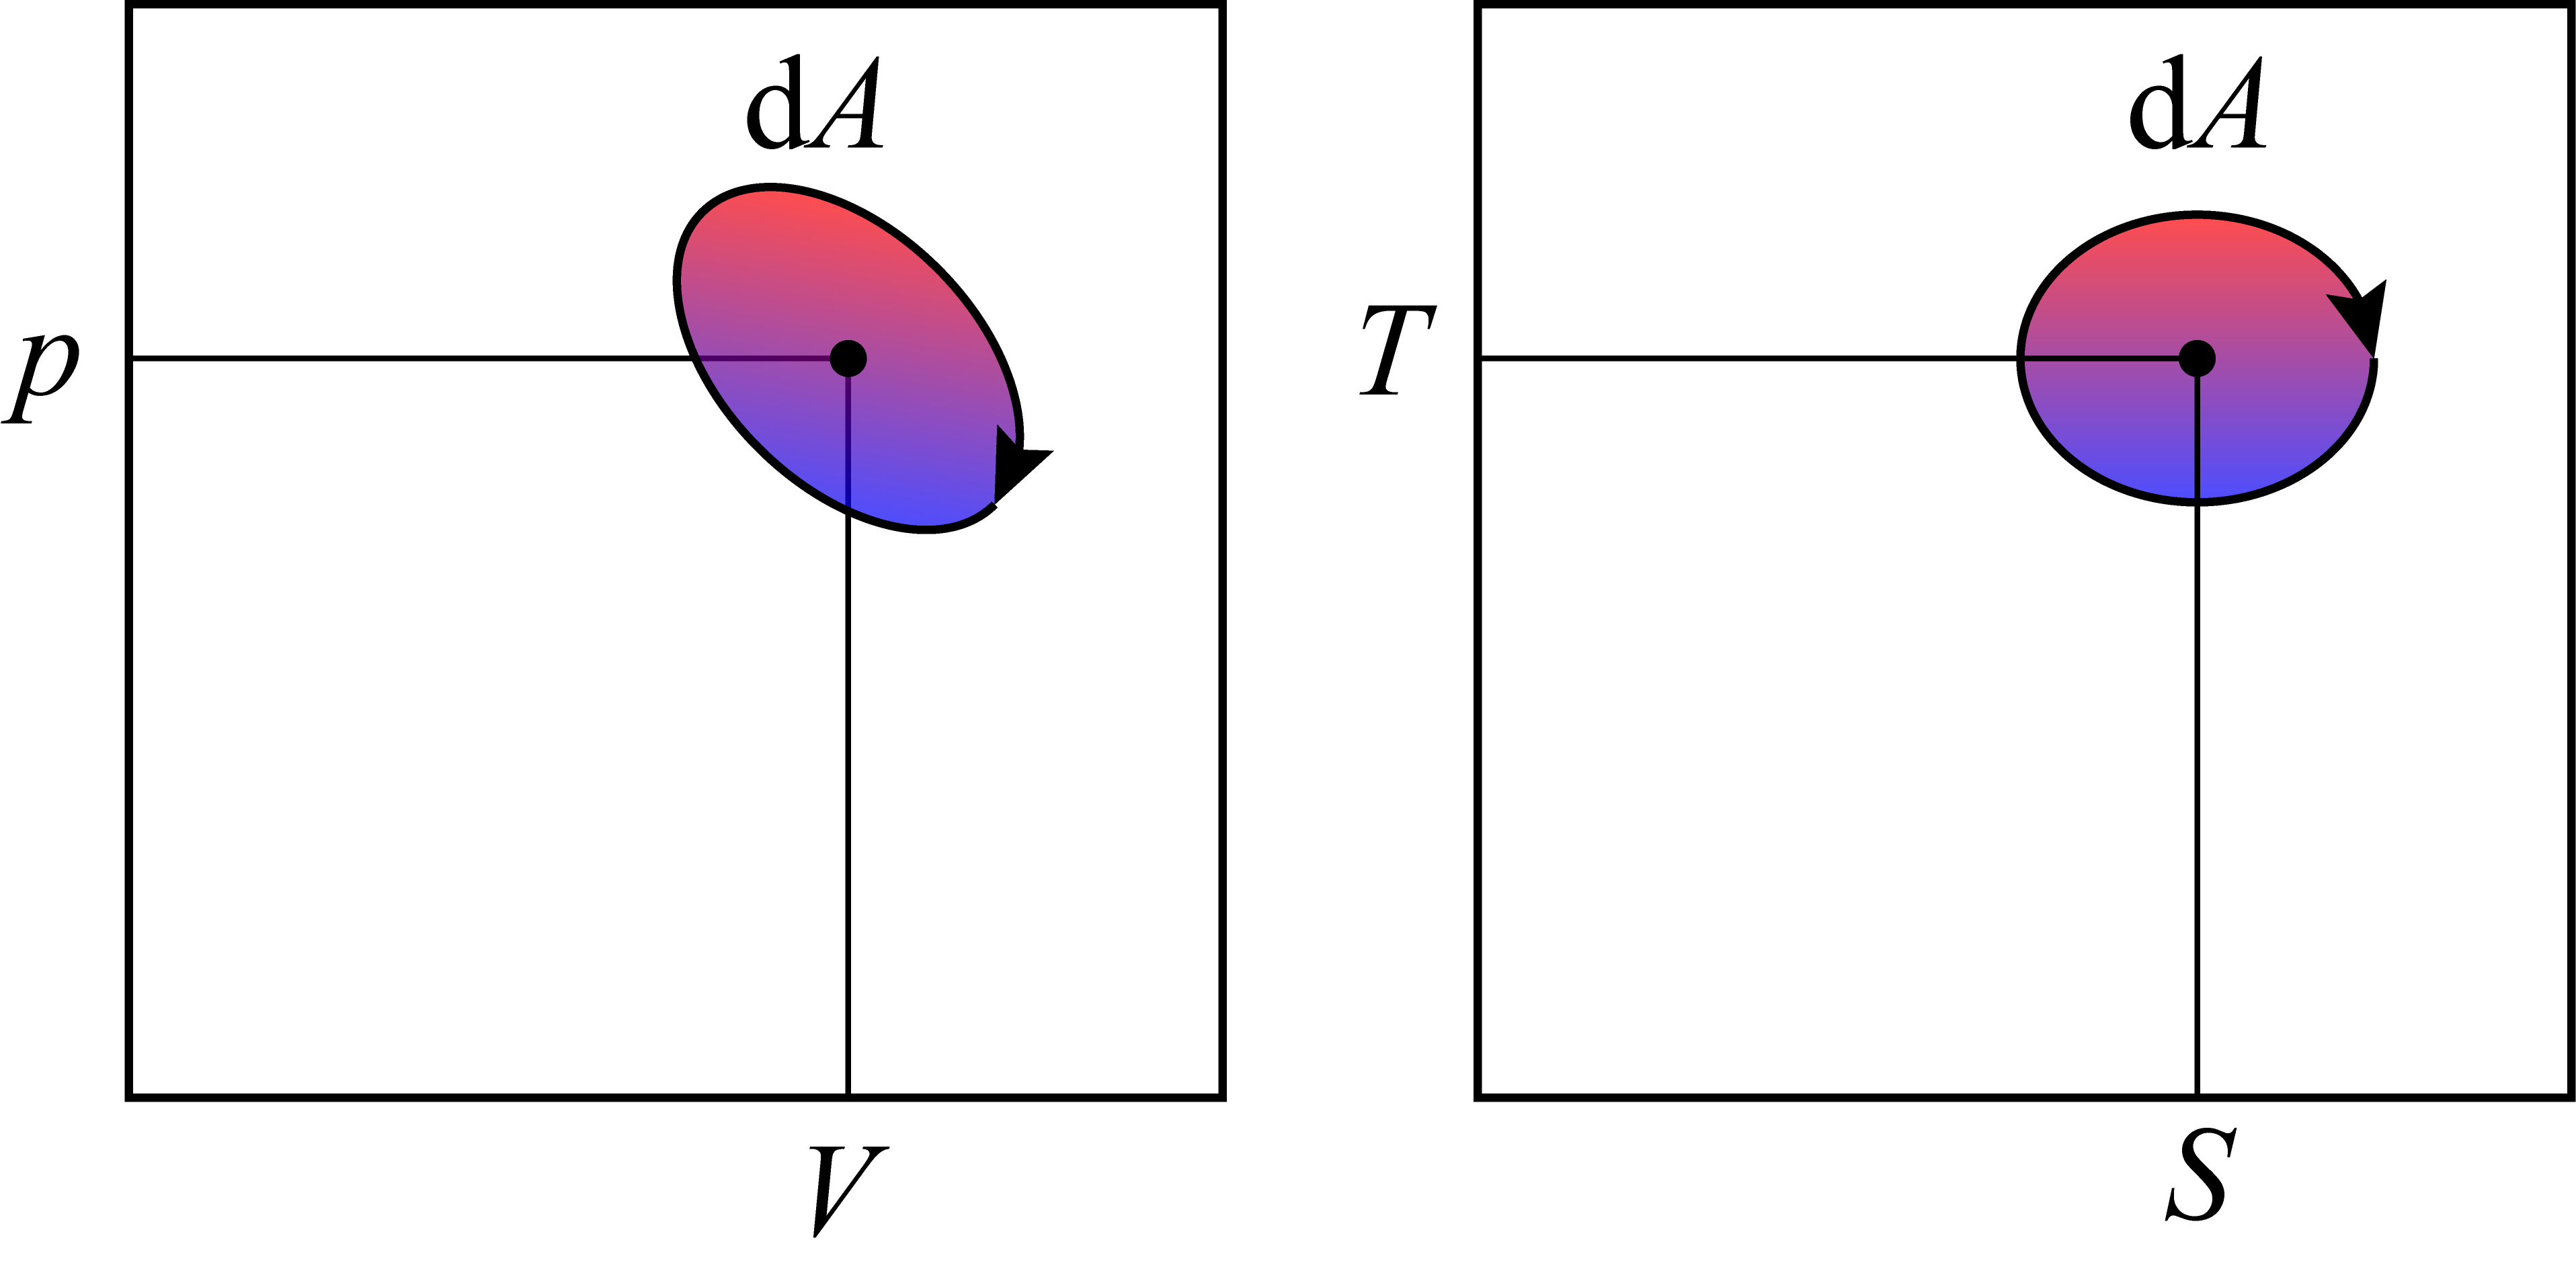
\includegraphics[width=8cm]{image/5-2-17.png}
\caption{循环过程的做功与吸热相等}
\end{wrapfigure}
如何理解这些关系?\,它们实际上都来自热力学规律对从$p,\,V$确定$T,\,S$的映射的性质.\,如果我们画出$p-V$图与$T-S$图,\,则两个图形上的点一一对应.\,$p-V$图上的一个闭区域的面积必须和对应的$T-S$图上的面积相等.\,这是因为其边界对应的循环过程的吸热与做功就是两个面积,\,由热一两者必然相等.\,这种性质在数学上表述为\emph{雅可比行列式}(Jacobian determinant)必须等于一:
\[\frac{\partial(T,S)}{\partial(p,V)}=\begin{vmatrix}\dfrac{\partial T}{\partial p} & \dfrac{\partial S}{\partial p} \\[8pt] \dfrac{\partial T}{\partial V} & \dfrac{\partial S}{\partial V}\end{vmatrix}=\left(\frac{\partial T}{\partial p}\right)_V\left(\frac{\partial S}{\partial V}\right)_p-\left(\frac{\partial S}{\partial p}\right)_V\left(\frac{\partial T}{\partial V}\right)_p=1\]

而且是$+1$,\,这代表循环的顺时针与逆时针在映射下保持不变.\,对于符号$\partial(p,V)$,\,我们理解为点$(p,V)$周围的一小块邻域的面积大小.\,这样这个式子就是一个直观的微商式,\,而上式两个面积比之所以可以用行列式来表示,\,是因为在$p-V$图上$(p,V)$点移动$\ud p$,\,在$T-S$图上移动矢量$(\dfrac{\partial T}{\partial p},\dfrac{\partial S}{\partial p})\ud p$,\,若移动$\ud V$,\,则在$T-S$图应移动$(\dfrac{\partial T}{\partial V},\dfrac{\partial S}{\partial V})\ud V$,\,那么在$p-V$图上由两个移动构成的矩形面积为$\ud p\ud V$,\,而$T_S$图上面积应为$\left|(\dfrac{\partial T}{\partial V},\dfrac{\partial S}{\partial V})\times(\dfrac{\partial T}{\partial V},\dfrac{\partial S}{\partial V})\right|\ud p\ud V$,\,根据代数知识这个叉乘就等于以上行列式.

也是基于这个认识,\,不难写出:
\[\left(\frac{\partial T}{\partial V}\right)_S=\frac{\partial(T,S)}{\partial(V,S)}=\frac{\partial(p,V)}{\partial(V,S)}=-\frac{\partial(V,p)}{\partial(V,S)}=-\left(\frac{\partial p}{\partial S}\right)_V\]

其他三个麦克斯韦关系也可以依据这个方法进行推导.\,在$p-V$图和$T-S$图上应该如何直观理解这个式子还请读者自己思考.

\subsection{若干定理的证明}
\vspace{0.5cm}
\subsubsection{\hei 能态定理}
对于$p-V$体系,\,若给出状态方程,\,则能量关于状态参量的偏导数有以下条件必须满足:
\[\left(\frac{\partial U}{\partial V}\right)_T=T\left(\frac{\partial p}{\partial T}\right)_V-p\]

\npg{-3cm}
{\hei 证法一:}

利用$U(S,V)$是\emph{特性函数}(characteristic function),\,用它可以表示出任意状态参量与其偏导数:
\[p=-U_V\quad,\quad T=U_S \]
\[\left(\frac{\partial p}{\partial T}\right)_V=\left(\frac{\partial S}{\partial T}\right)_V\cdot\left(\frac{\partial p}{\partial S}\right)_V=-\left(\frac{\partial S}{\partial T}\right)_V\cdot U_{SV}\]
\[\ud T=\ud U_S=U_{SS}\ud S+U_{SV}\ud V\quad \Rightarrow \quad \left(\frac{\partial S}{\partial T}\right)_V=\frac{1}{U_{SS}}\; ,\;\left(\frac{\partial p}{\partial T}\right)_V=-\frac{U_{SV}}{U_{SS}}\]
从而等式右边为:
\[T\left(\frac{\partial p}{\partial T}\right)_V-p=U_V-\frac{U_S U_{SV}}{U_{SS}}\]

而等式左边为:
\[\left(\frac{\partial U}{\partial V}\right)_T=\left(\frac{\partial U}{\partial V}\right)_S+\left(\frac{\partial U}{\partial S}\right)_V\cdot\left(\frac{\partial S}{\partial V}\right)_T\]
\[\ud T=\ud U_S=U_{SS}\ud S+U_{SV}\ud V\quad \Rightarrow \quad \left(\frac{\partial S}{\partial V}\right)_T=-\frac{U_{SV}}{U_{SS}}\]

代入,\,即有:
\[\left(\frac{\partial U}{\partial V}\right)_T=U_V-\frac{U_S U_{SV}}{U_{SS}}\]
从而两式相等.

\vspace{1cm}
{\hei 证法二:}

方程以$T,\,V$作为自变量,\,故考虑自由能$F=U-TS$,\,它恰好以$T,\,V$为自变量时为特性函数,\,有:
\[\left(\frac{\partial U}{\partial V}\right)_T=\left(\frac{\partial F}{\partial V}\right)_T-T\left(\frac{\partial S}{\partial V}\right)_T=-p+T\left(\frac{\partial p}{\partial T}\right)_V\]

后一步推导用到了麦克斯韦关系.

\vspace{1cm}
{\hei 证法三:}

\begin{wrapfigure}[11]{o}[-10pt]{8cm}
\centering
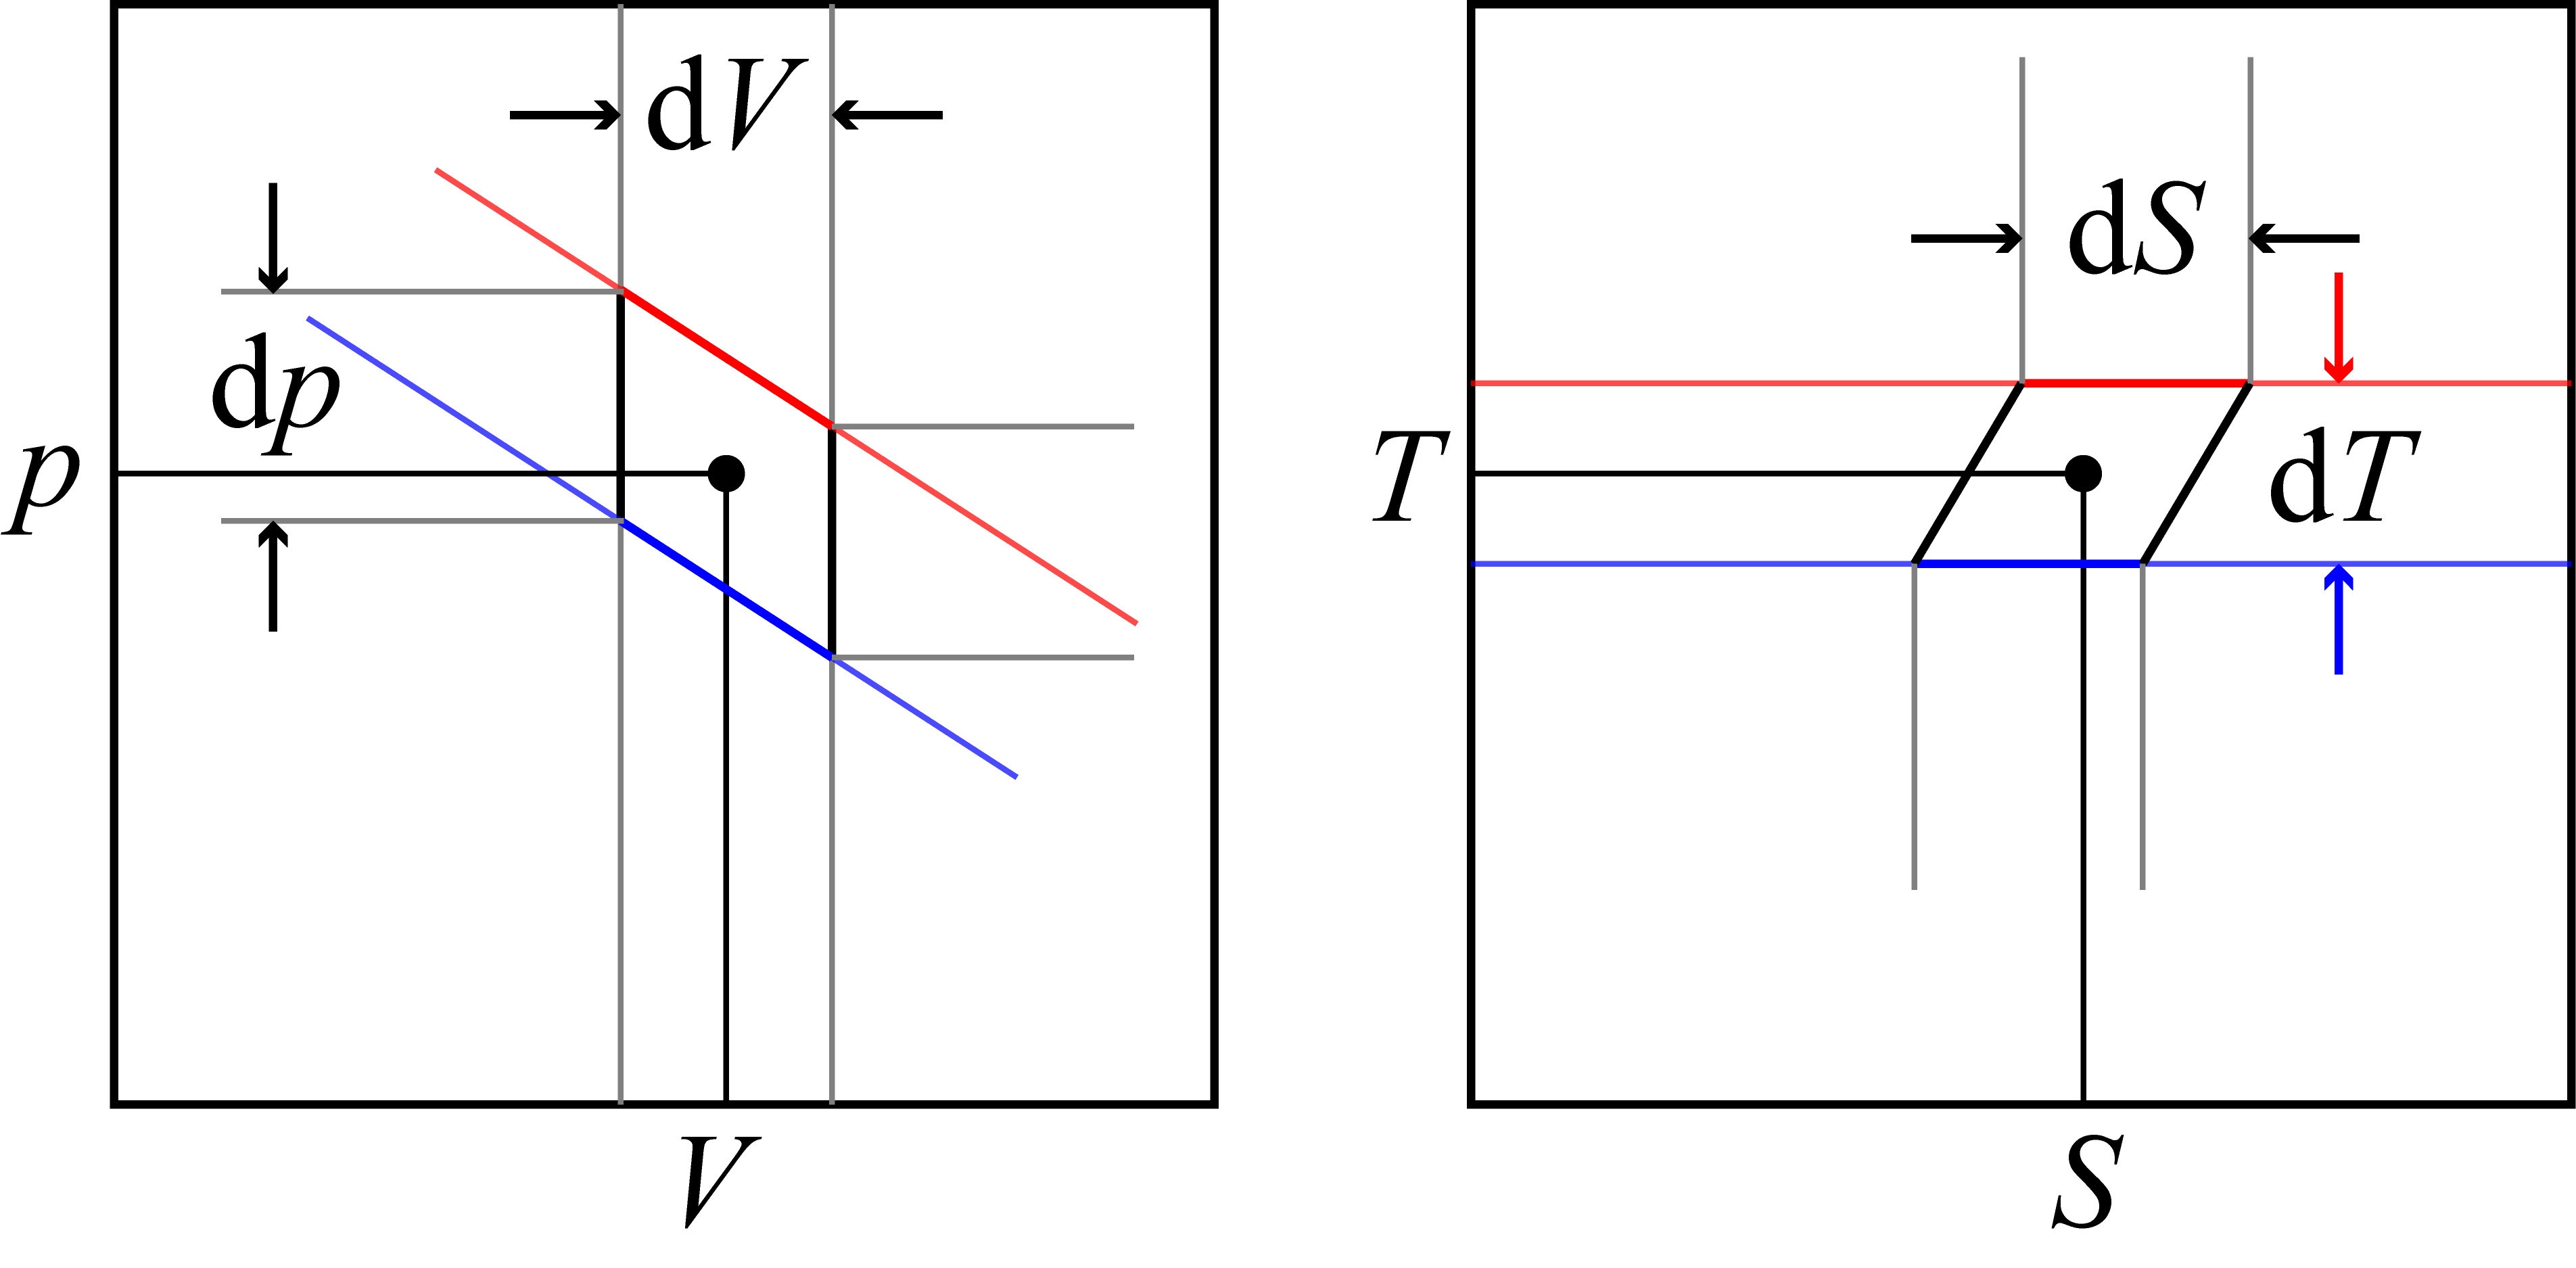
\includegraphics[width=8cm]{image/5-2-18.png}
\caption{构造循环过程证明能态定理}
\end{wrapfigure}
构造在两根相差$\ud V$的等体线和相差$\ud T$的等温线之间的循环过程.\,这不是一个卡诺循环,\,但依然近似有两个等温过程中的吸放热定义的效率为:
\[\eta=1-\frac{\dbar Q_{\rm L}}{\dbar Q_{\rm H}}=\frac{\delta \dbar Q}{\dbar Q}=\frac{\ud T}{T}\]

这一点从这个循环对应的$T-S$图中可以看出来,\,小段红线下方的面积与小段蓝线下方的面积,\,由于微元过程近似为平行四边形,\,两个面积的底$\ud S$相等,\,面积差即为平行四边形的面积$\ud T \ud S$,\,而吸放热约为$T\ud S$,\,它们的比就是上式.

现在我们把注意力集中在左图中.\,在等体过程中增加的压强为$\left(\dfrac{\partial p}{\partial T}\right)_V\ud T$,\,从而过程做功为:
\[\dbar W=\left(\frac{\partial p}{\partial T}\right)_V\ud T\ud V\]

而两个等温过程中的吸热,\,由热力学第一定律:
\[\dbar Q=p\ud V+\left(\frac{\partial U}{\partial V}\right)_T \ud V\]

把两式与循环效率比对:
\[\frac{\dbar W}{\dbar Q}=\frac{\ud T}{T}\]

即得:
\[\left(\frac{\partial U}{\partial V}\right)_T=T\left(\frac{\partial p}{\partial T}\right)_V-p\]

\vspace{1cm}
把这个式子用于理想气体的物态方程:
\[pV=\nu RT\quad \Rightarrow \quad \left(\frac{\partial U}{\partial V}\right)_T=0\]

可见理想气体的内能只和温度有关是由物态方程决定的.\,而满足该物态方程的其他气体模型也需要符合这一点,\,所以内能对温度的偏导数仍然符合等体热容的定义,\,但热容一般是温度的函数:
\[U=\nu \int C_{mV}(T)\ud T\]

实际气体,\,一方面在高密度,\,高温度情况下其状态方程会偏离理想物态方程的形式,\,另一方面,\,多原子分子气体其内能-温度关系在常温-低温区一般体现为温度的单调递增函数的形式,\,而在某些温度区间达到一些近似不变的平台.\,这反应了气体内部自由度的量子本质.\,在一种近似的模型处理中,\,我们可以让$T<T_c$时摩尔等体热容为$C_{mV}=\dfrac{i}{2} R$,\,而$T>T_c$时摩尔等体热容为$C_{mV}=\dfrac{f}{2} R$,\,而在$T=T_c$附近的微小区间内不仅热容迅速升高,\,内能也突然从$\dfrac{i}{2}\nu RT_c$上升到$\dfrac{f}{2}\nu RT_c$\footnote{事实上由于需要吸热而温度不变,\,这个过程热容是发散的.}.\,这实际上是一种相变-期间两种热容的分子可以视为共存,\,详见第四章相与相变的内容.

这种情况也很容易推广到一个类似体系中:\,液膜的热力学系统.\,在此时热力学基本方程写作:
\[\ud U=T\ud S+\sigma \ud A\]

可见在这儿表面张力系数$\sigma$是广义力,\,广义坐标是表面积$A$.\,故我们可以写出:
\[\left(\frac{\partial U}{\partial A}\right)_T=\sigma-T\left(\frac{\partial \sigma}{\partial T}\right)_A\]

一般$\sigma$是温度$T$的函数,\,只不过与理想气体情况不太相同的是,\,$\sigma$依赖于$T$但一般不依赖于液面表面积$A$,\,液膜的拉伸改变的是膜的厚度,\,而表面层永远是膜的两个表面上极薄的一层,\,它的性质不会改变,\,从而不会改变表面张力系数(详见下一章液体与固体的性质).\,事实上,\,此时我们注意到自由能的性质为:
\[\ud F=-S\ud T+\sigma \ud A\]

而$\dfrac{\partial \sigma}{\partial A}=0$意味着:
\[\left(\frac{\partial F}{\partial A}\right)_T=\sigma(T) \quad;\quad \left(\frac{\partial^2 F}{\partial A^2}\right)_T=0\]

这意味着$F=\sigma(T)A+f(T)$,\,对于$f(T)$,\,显然与表面现象没有关系,\,因为当面积$A=0$时这一项仍然存在,\,说明不是因为表面现象引起的,\,实验时与理论计算都应该扣除.\,从而我们给出:
\[F=\sigma A\]

也就是说平时说的表面能在热力学下实际上是自由能.\,它恰恰是表面积$A$的广延量.\,而熵应该为:
\[S=-\left(\frac{\partial F}{\partial T}\right)_A=-\sigma'A\]

最后再代入到$U=F+TS$,\,得:
\[U=(\sigma-T\sigma')A\]

内能与面积的比例系数不是$\sigma$,\,但由$\sigma$决定,\,意料之外,\,情理之中.\,这意味着等温地拉伸液膜是需要吸放热的,\,从微观机理上来看,\,熵必须大于零,\,从而$A$增加熵应该也要增加.\,从以上熵的表达式来看必然有:
\[\sigma'<0\]

从而我们得出了温度升高表面张力系数减小的结论.\,微观上看,\,温度升高导致分子从液相通过表面层到气相更简单,\,表面层变薄,\,所以表面能减小.\,从而拉伸液膜是要吸热的.\,而如果面积不变,\,而温度升高,\,我们得到等面积热容为
\[C_A=-T\sigma'' A\]

\begin{wrapfigure}[12]{o}[-10pt]{6cm}
\centering
\vspace{-0.3cm}
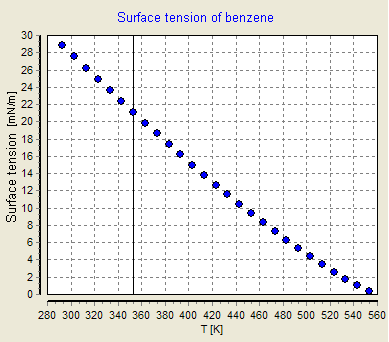
\includegraphics[width=6cm]{image/5-2-19.png}
\caption{苯的$\sigma\sim T$关系}
\end{wrapfigure}
对于一般的有机液体有经验公式:
\[\sigma=\sigma_0(1-\frac{T}{T_C})^n\]

一般$n\simeq \dfrac{11}{9}$,\,从而我们发现$C_A<0$\footnote{热力学预言简单的$p-V$系统如果热容小于零将是不稳定的\ca 传热将使得局部高温更高,\,低温更低.}.\,这没什么奇怪的,\,要知道液膜的表面层是依附于内部的液体而存在的.\,所以既使增加$A$对内部液体没有影响,\,升温绝对是对两侧的液,\,气相产生影响的.\,这个热容将被包含在正的较大的液体气体热容中.\,它的减小可以理解为温度升高时表面层变薄而直接减少内能的缘故.\,另外,\,在$T=T_C$处$\sigma$减小到零,\,内能与自由能也都减小到了零.\,这也是预料之中的.\,这一点就是液相与气相共存的临界点.\,第四章相与相变将仔细研究这个现象.

\vspace{0.5cm}
\subsubsection{\hei 物性函数间关系}
除了两个热容$C_{mp},\,C_{mV}$,\,实验中容易测得的量一般只能是$p,\,V,\,T$.\,从而连带着可以测的还有在上一章理想气体的过程这一节中介绍的各种\emph{物性函数}(material property function):\,膨胀系数$\alpha$,\,压强系数$\beta$和压缩系数$\kappa$.\,不同的过程中这些量间有关系:
\[\alpha_X=-p\beta_X\kappa_X\]
\[\alpha_p=p\beta_V\kappa_T\]
\[\gamma=\frac{C_{p}}{C_{V}}=\frac{\kappa_T}{\kappa_S}\]
\[C_{p}-C_{V}=pVT\alpha_p\beta_V\]

其中下标$X$表示一个任意的过程.

\vspace{0.3cm}
{\hei 证明:}

二自由变量的$p-V$系统引入一个过程方程后变为一自由变量,\,所有变化的微元互相之间都成正比,\,即:
\[\ud p=\lambda_p \ud x\; , \; \ud V=\lambda_V \ud x\; , \; \ud T=\lambda_T \ud x\]

其中$x$作为过程参数反应过程发生的程度.\,从而三个$X$过程的响应函数分别为:
\[\alpha_X=\frac{1}{V}\left(\frac{\partial V}{\partial T}\right)_X=\frac{\lambda_V}{V\lambda_T}\]
\[\beta_X=\frac{1}{p}\left(\frac{\partial p}{\partial T}\right)_X=\frac{\lambda_p}{p\lambda_T}\]
\[\kappa_X=-\frac{1}{V}\left(\frac{\partial V}{\partial p}\right)_X=-\frac{\lambda_V}{V\lambda_p}\]

从而得到待证第一式.\,而第二个式子的区别在于它不依赖于某个过程,\,而是直接从物态方程中得出:
\[F(p,V,T)=0\quad \Rightarrow \quad F_p\ud p +F_V \ud V +F_T \ud T=0\]
\[\Rightarrow \quad \alpha_p=-\frac{F_T}{VF_V}\, , \, \beta_V=-\frac{F_T}{pF_p}\, , \, \kappa_T=\frac{F_p}{VF_V}\]

即可证明第二式.\,这两个过程都仅仅是数学恒等式,\,不依赖于任何体系的物理性质.\,而第三个式子则需要热二的相关推论来推导.\,首先注意到一下关于两个热容的定义是与之前说法等价的:
\[C_{V}=\left(\frac{\partial U}{\partial T}\right)_V=T\left(\frac{\partial S}{\partial T}\right)_V\quad ;\quad C_{p}=\left(\frac{\partial H}{\partial T}\right)_p=T\left(\frac{\partial S}{\partial T}\right)_p\]

从而利用雅可比行列式的方法:
\[\frac{C_{p}}{C_{V}}=\frac{\left(\dfrac{\partial S}{\partial T}\right)_p}{\left(\dfrac{\partial S}{\partial T}\right)_V}=\frac{\partial(S,p)}{\partial(T,p)}\cdot\frac{\partial(T,V)}{\partial(S,V)}=\frac{\partial(T,V)}{\partial(T,p)}\cdot\frac{\partial(S,p)}{\partial(S,V)}=\frac{\left(\dfrac{\partial V}{\partial p}\right)_T}{\left(\dfrac{\partial V}{\partial p}\right)_S}=\frac{\kappa_T}{\kappa_S}\]

这就是第三式,\,而最后一式则考虑$(V,T)$为自变量:
\[C_p-C_V=T\left(\frac{\partial S}{\partial T}\right)_p-T\left(\frac{\partial S}{\partial T}\right)_V=T\left(\frac{\partial S}{\partial V}\right)_T\left(\frac{\partial V}{\partial T}\right)_p=T\left(\frac{\partial p}{\partial T}\right)_V\left(\frac{\partial V}{\partial T}\right)_p=pVT\alpha_p\beta_V\]

期间用了一次麦克斯韦关系.\,至此四个关系式都得证.

\vspace{0.5cm}
\subsubsection{\hei 吉布斯-亥姆霍兹方程}

吉布斯-亥姆霍兹方程(Gibbs-Helmholtz equation)用来确定化学反应中的吸放热(实际上是焓变)与吉布斯自由能的变化间的关系,\,而吉布斯函数又和化学反应发生的方向,\,化学平衡的位置紧密相关.\,这个关系写作:
\[\left(\frac{\partial}{\partial T}\right)_p \frac{G}{T}=-\frac{H}{T^2}\]

\vspace{0.3cm}
{\hei 证明:}

实际上:
\[H=G+TS=G-T\left(\frac{\partial G}{\partial T}\right)_p=-T^2[G\left(\frac{\partial}{\partial T}\right)\frac{1}{T}+\frac{1}{T}\left(\frac{\partial}{\partial T}\right)G]=-T^2\left(\frac{\partial}{\partial T}\right)\frac{G}{T}\]

这就是上式.\,相似的关系我们还可以写出:
\[\left(\frac{\partial}{\partial T}\right)_V \frac{F}{T}=-\frac{U}{T^2}\]
\[\left(\frac{\partial}{\partial V}\right)_T \frac{F}{V}=-\frac{G}{V^2}\]
\[\left(\frac{\partial}{\partial p}\right)_T \frac{G}{p}=-\frac{F}{p^2}\]

\subsection{自由能的含义}

我们先讨论亥姆霍兹自由能,\,对于双参数描述的简单系统,\,此时热力学基本关系牢固地成立,\,不管过程是否准静态:
\[\ud U=T\ud S-p\ud V\]

但对于非双参数的,\,比如我们考虑两种气体的相互扩散,\,初态与末态似乎其表现出来的性质是类似的.\,比如标准状态下$1{\rm mol}$正氢与$1{\rm mol}$仲氢混合均匀.\,如果视为一个$p-V$系,\,整个过程前后等温,\,等压,\,等体,\,但熵增.\,这类问题上式就不再是一个等式.\,究其本质,\,在与内部发生的各种过程的各种不平衡与耗散的因素造成的自发熵产生.\,体系总是受迫地远离平衡态,\,而有自发地从非平恒态回到平衡态.\,为了简化,\,我们假设系统与外界的热,\,功交换仍然是准静态且无耗散的\footnote{为了表述的简化我们让体系的每处都处于共同温度$T$而每个与外界交换的体积功都发生在共同压强$p$处,\,只要我们愿意对于较复杂的系统我们随时都可以把下面式子写为:\[\Delta U \leq \sum_i T_i\Delta S_i -\sum_j p_j\Delta V_j\]},\,熵产生仅仅发生在体系内部.\,此时上式应该写为:
\[\Delta U \leq T\Delta S -p\Delta V\]

这是因为外界对系统做功仍然为$\Delta W=-p\Delta V$,\,但根据克劳修斯不等式系统从外界吸热满足$\Delta Q\leq T\Delta S$.\,而最终$\Delta U=\Delta Q+\Delta W$的缘故.\,注意到克劳修斯不等式的本质就是系统与外界一起看成一个整体的熵增原理.\,它是普适的,\,对任意复杂体系都适用的统计规律.\,上式也通常写成
\[\Delta S\geq \frac{\Delta U}{T}+\frac{p\Delta V}{T}\]

上式也与熵增原理兼容,\,等体,\,绝热的体系自然可以认为是孤立的,\,它内能不变,\,从而上式给出了$\Delta S>0$.\,但上式实际上比熵增原理更强.\,因为即使如果对于$V$增大的过程,\,即使不可逆,\,上式对理想气体也应该严格成立,\,但对于一般多内部参量的$p-V$系统上式则可以取不等号.\,上式还给出了平衡态的条件:\,我们可以在不改变体系总内能和总体积的情况下分配各部分所占的内能和体积,\,如果可以通过某种分配方式让熵增加,\,则体系会自发地往这个方向演化.\,直至熵达到它的极大值,\,对应热力学平衡态.\,这叫做\emph{最大熵原理}(principle of maximum entropy).

从内能的相似表达式中可以得到完全一致的结论,\,不过此时我们要保持熵$S$与体积$V$不变.\,而结论是对应的\emph{热力学势}(thermodynamic potential)\ca 内能取最小.\,对应的原理为\emph{最小能原理}(principle of minimum energy).\,从内能出发的这个结论有些不足之处:\,熵理论上计算公式复杂,\,实际操作上又因为无法直接控制其不变而没有意义,\,且难以用微观统计观点诠释的熵的概念解释.\,所以仅仅有较为好的热力学理论价值.

亥姆霍兹自由能的优势就体现在这儿了,\,由于$F=U-TS$,\,在等温的条件下我们写出:
\[\Delta F\leq-S\Delta T-p\Delta V\]

从而这个关系式对应的平衡判据为\ca 在等温等体情况下自由能必须极小.\,这个式子实际上经常意味着纯粹的机械平衡.\,例如我们还记得液膜的自由能就是$F=\sigma A$,\,而后一项$-p\Delta V$理解为$\Delta W$,\,这个原理就是:\,在一定温度下固定边界(外界不做功)的液膜的面积要收缩到最小.\,利用\emph{变分法}(calculus of variation)我们可以把这个最小曲面确定下来.\,我们将在下一章介绍液体表面张力时介绍相关概念.

如果放宽条件,\,允许系统在不变的温度下对外做功$\Delta W'=-\Delta W=p\Delta V$,\,那么两边同时积分给出:
\[W'\leq F_{\rm initial}-F_{\rm final}\]

等号成立时,\,这就是个机械能守恒,\,自由能$F$具有势能的含义.\,而不等号的存在意味着热力学系统的不可逆性.\,上式又被称为\emph{最大功原理}(principle of maximum work).\,虽然名称与上面两个原理相似,\,但这个原理不是用作一个平衡判据,\,而是用于实际过程,\,工程上往往把整个系统与外界和合自由能称为\emph{火用}\footnote{笔者电脑字库里没有这个字orz.}(exergy).

接着我们讨论吉布斯自由能$G$.\,同样,\,吉布斯自由能的能量最小判据在等温等压的条件下被写作:
\[\Delta G\leq -S\Delta T +V\Delta p\]

也就是说,\,在等温,\,等压的过程中吉布斯自由能$G$总是取到它的极小值.\,而等温等压的过程又常常是各种化学反应发生的初末态要符合的条件.\,此式在判断化学反应的发生方向上极为有用.\,在各种燃烧的模型中,\,我们发现气体发生化学反应体积膨胀对外做的功不全由体积功$p_0\Delta V$表示,\,这是因为把外界压强(初末态平衡压强)与过程中气体压强划等号的不合理.\,此时还会有其他形式的机械功输出,\,要么转化为气体的动能,\,要么利用起来推动活塞对外做功.\,这一部分功称为非体积功$W''$,\,由于$W'=W''+p\Delta V$,\,我们通过上面的亥姆霍兹自由能的最大功原理写出等温等压下的吉布斯自由能的最大功原理:
\[W''\leq G_{\rm initial}-G_{\rm final}\]

\subsection{化学势}
最后我们再考虑一下粒子数可变的系统.\,对于理想气体类似的仅由$p-V$决定的系统在考虑粒子数变化后将有三个独立变化的状态参量.\,我们注意到粒子数$N$不变时:
\[\ud G=-S\ud T+V\ud p\]

而显然$G,\,S,\,V$恰好都是广延量,\,而作为自变量的$p,\,T$是两个强度量.\,这就是说,\,如果我们引入``每个粒子携带的吉布斯自由能''$\mu=\dfrac{G}{N}$,\,同样地,\,我们不假思索的把所有广延量平分到每个粒子上,\,用它们的小写表示,\,如$s,\,v,\,u,\,h,\,f$等等.\,研究吉布斯自由能便可以发现:
\[\ud \mu=-s\ud T+v\ud p\]
\[\ud G=\ud (N\mu)=-S\ud T+V\ud p+\mu \ud N\]

而如果研究内能便可以发现:
\[\ud u=T\ud s-p\ud v\]
\[\ud U=\ud (Nu)=NT\ud s-Np\ud v+ u\ud N=T\ud (Ns)-p\ud(Nv)+(u-Ts+pv)\ud N=T\ud S-p\ud V +\mu \ud N\]

另外两个热力学势是类似的:
\[\ud F=-S\ud T-p\ud V +\mu \ud N\]
\[\ud H=T\ud S+V\ud p+\mu \ud N\]

从中可以看出$\mu$具有某种特殊的含义,\,我们把这个量叫做\emph{化学势}(chemical potential).\,它是在准静态的等温等压过程中向体系添加一个粒子外界需要做的非体积功.\,它与相之间的平衡与转化问题息息相关.\,如一个在等温等压条件下自发进行的化学反应过程${\rm A \longrightarrow B}$,\,我们如果不对体系做非体积功,\,也不去吸收非体积功,\,那么根据最小功原理吉布斯自由能必须减小.\,也就是${\rm A}$的化学势必须比${\rm B}$的化学势高可以利用化学势的差对外输出机械功,\,这便是内燃机的原理.\,达到平衡时有$\mu_A=\mu_B$,\,此时两相之间的粒子交换已经是准静态的过程.\,不会造成过程的不可逆性.

在引入化学势后对于共存的,\,或多相混合的,\,甚至非均匀的$p-V$系统我们统一地写出热力学的基本关系式:
\[\ud U=T\ud S-p\ud V+\sum_\alpha \mu_\alpha\ud N_\alpha\]

上式是一个恒等式,\,不再像之前的讨论那样由于缺少内部的参数而导致成为不等式.\,这一点容易理解,\,因为考虑到化学势实际上说明我们对不同的组分进行了区分,\,考虑到了实际$p-V$系统的内部构成而不是仅仅研究其宏观彻体性质.\,在这一点上,\,上式中各个量都是明确的微观含义,\,对于平衡态和下一节要介绍的近平衡态都是可以使用的.\,不会造成不相等的情形.


\section{近平衡态热力学*}

从古至今,\,物理学对\emph{非平衡态}(non-equilibrium state)的研究兴趣丝毫不亚于对平衡态的研究.\,著名的\emph{开尔文勋爵}({\it Lord Kelvin})就曾试图处理不可逆过程.\,直到20世纪三四十年代才有\emph{昂萨格}({\it Onsager})等人建立了\emph{近平衡态}(near-equilibrium)的热力学与统计理论.\,而在六七十年代又由\emph{普利高津}({\it Prigogine})等人对\emph{远离平衡态}(far from equilibrium)的研究而大放异彩.\,远离平衡态的性质将在本书的讨论范围外,\,我们在这儿对近平衡态中的线性特性做一个简介.

\subsection{线性输运现象}
当系统处于非平衡态时,\,系统内部一般存在压强,\,温度,\,浓度,\,电势梯度.\,分别将引起质量\footnote{这是黏滞现象,\,本书将不讨论},\,热量,\,粒子与电荷的迁移,\,称为\emph{输运现象}(transport phenomenon).\,形象地看这种因果关系,\,我们把各种非平衡的梯度称为\emph{力}(force),\,而导致的输运称为\emph{流}(flow).\,在力较小时流近似与力成正比,\,这个线性的区域正是近平衡态热力学所研究的区域.\,历史上人们相继发现了如下经验规律:

\subsubsection{\hei 傅里叶({\it Fourier\,})热传导定律}
\[\bs{J}_q=-\kappa\nabla T\]
其中\(\bs{J}_q\)表示热流密度.\,热交换是指通过非粒子交换,\,也非物质团集体运动而通过热接触,\,分子碰撞而交换的能量部分.\,而系数\(\kappa\)称为\emph{热导率}(thermal conductivity).

\subsubsection{\hei 菲克({\it Fick\,})扩散定律}
\[\bs{J}_n=-D_0\nabla n\]
其中\(\bs{J}_n\)表示粒子流密度.\,但为了热力学的统一处理我们又经常把上式写为:
\[\bs{J}_n=-D\nabla \mu\]
注意到\(\mu=\mu(n,T)\),\,一般一定温度下化学势都是与浓度正相关的,\,两种定义因此而能够互相换算\(\displaystyle D_0=D\left(\frac{\partial \mu}{\partial n}\right)_T\),\,仅仅是\emph{扩散率}(diffusivity)的取法不同.\,然而如果不等温的情形如何处理?\,这不会带来问题,\,因为温度梯度也能造成粒子流,\,见下.

\subsubsection{\hei 欧姆({\it Ohm\,})定律}
\[\bs{J}_e=-\sigma\nabla \varphi\]
其中\(\bs{J}_e\)表示电流密度.\,而\(\sigma\)为导体的\emph{电导率}(electrical conductivity).

\subsubsection{\hei 索瑞({\it Soret\,})效应}
温差传热与浓度差传粒子的现象存在耦合,\,温度差(而不是浓度差)也将导致粒子的扩散.\,这个效应称为\emph{热迁移}(thermophoresis)或\emph{热扩散}(thermodiffusion).\,类似的可以由以下经验公式表示:
\[\bs{J}_n=-D_T\nabla T\]

其中\(D_T\)称为\emph{热扩散率}(thermodiffusivity).\,从而在傅里叶热传导实验中,\,如图\ref{fig5-2-20}左,\,在温度梯度下实际上存在着热流与粒子流两种同时存在的现象.
\begin{figure}[H]
\centering
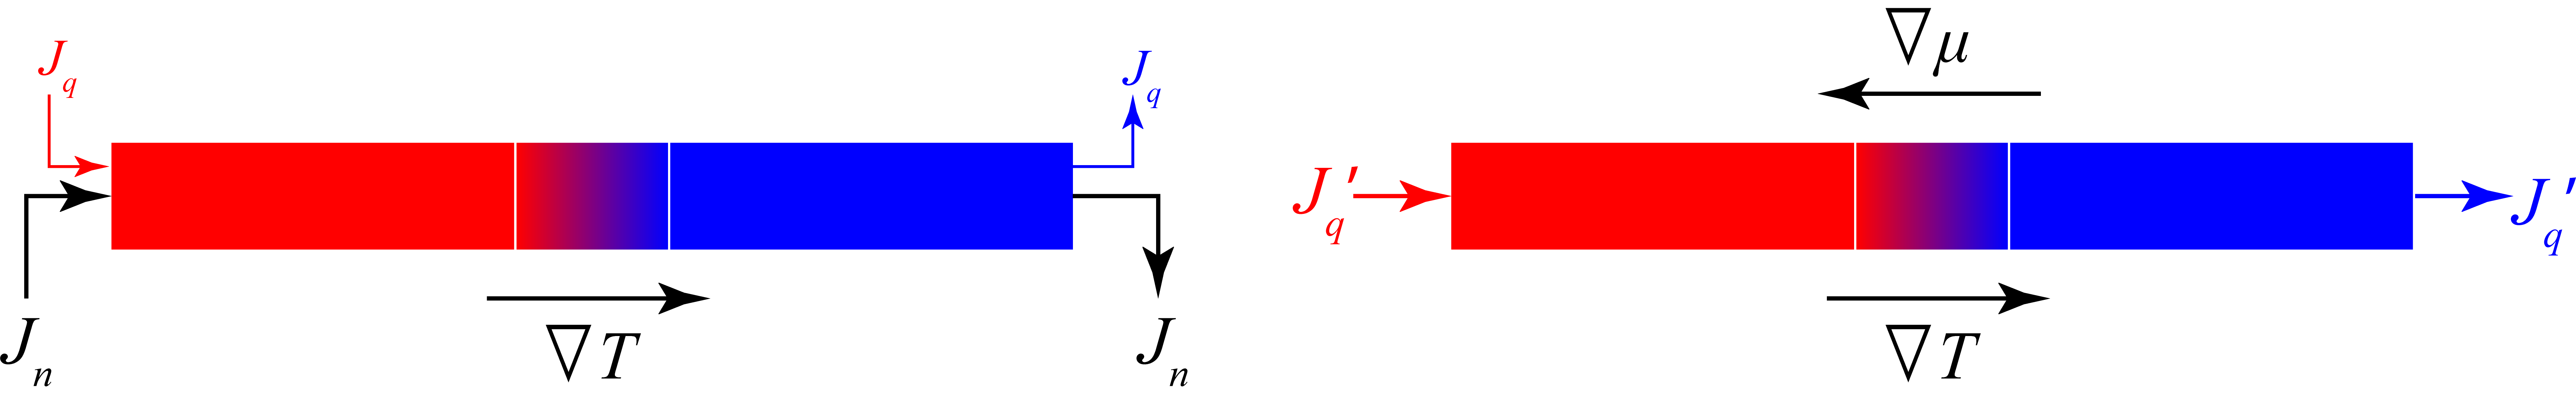
\includegraphics[width=16cm]{image/5-2-20.png}
\caption{Soret效应与Dufuer效应}\label{fig5-2-20}
\end{figure}

\subsubsection{\hei 杜福尔({\it Dufuer\,})效应}
如图\ref{fig5-2-20}右所示,\,在傅里叶热传导实验中阻断两侧的粒子流,\,那么由于热扩散现象的存在将造成两侧粒子的浓度差.\,两个效应由此产生的粒子流也因此而达到平衡而抵消.\,在此时对热流进行测量,\,其值将不同于有粒子流时的值,\,这可以被解释为由于粒子浓度梯度所造成的.\,经验规律可以写为:
\[\bs{J}_q-{\bs{J}_q}^\prime=\kappa_\mu\nabla\mu\]

\subsubsection{\hei 伽伐尼({\it Galvani\,})接触电势差}

金属内的电子体系不是一个简单的体系,\,在量子理论建立后才有\emph{能带理论}(energy band theory)能给出电子性质的正确描述.\,一般来讲,\,不同金属内的电子可以认为具有不同的化学势\(\mu_i\).\,此时如果让两种金属\(1\)与\(2\)相互接触,\,化学势高的金属,\,设为\(1\),\,其电子将自发地向化学势低的金属\(2\)上运动.\,这直接改变的不是化学势,\,而是更直接地导致了电磁学的结果---\(2\)上电势降低而\(1\)上电势升高.\,我们可以引入\emph{电化学势}(electrochemical potential)来表示两种驱动电子运动的效果的和,\,达到平衡时应有:
\[\bar{\mu}_1=\bar{\mu}_2\quad ; \quad \bar{\mu}_i=\mu_i-e\varphi_i\]

这一点也很好理解,\,\(\mu\)的含义为从无穷远移动一个电荷进入导体中外界所需要做的功,\,现在只需要把整体电荷分布所带来的电势能改变所需要的功也计及在内即可.\,上式给出了两种金属的\emph{接触电势差}(contact potential difference):
\[\varphi_1-\varphi_2=e(\mu_1-\mu_2)\]

然而它既不能产生回路电流,\,甚至也不能被直接测量:\,如果把第三种金属制作的电极加在两种金属两端,\,由于三个界面上都有接触电势差而使得第三种金属的两个电极上电势差为零.

\subsubsection{\hei 塞贝克({\it Seebeck\,})效应}
1821年物理学家塞贝克发现由两种材料的导线构成的闭合回路如果把两个连接点置于不同的温度环境下则会使得小磁针偏转.\,他把这个效应称为``热磁效应'',\,这是因为当时人们对电磁现象之间的联系缺乏认识,\,毕竟恰好在几乎同时奥斯特({\it \O rsted\,})才发现电流能够产生磁场.\,之后奥斯特就意识到这个现象是典型的热电耦合现象,\,展开了人们对热电耦合现象研究的序幕.\,类似于温差传热与浓度差传粒子的耦合,\,这个现象实际上是有以下经验规律:
\[\bs{J}_e=-\sigma \eta\nabla T\]

其中\(\eta\)被称为\emph{塞贝克系数}(Seebeck coefficient),\,而实际温差电现象有以下特点:\,温差电动势不依赖于导线的长度,\,不依赖于导线上温度的分布,\,既使中间有连接第三种材料的导线,\,只要连接点等温,\,也不影响温差电动势的大小.\,这很容易理解.\,首先意识到接触电势差不会带来电动势,\,其次在第\(i\)段导线上的非静电力为:
\[\bs{J}_e=\sigma \bs{K}\quad \Rightarrow \quad \bs{K}=-\eta_i\nabla T\]

从而两端的总电动势为:
\[\mathcal{E}_i=\int_{H_i}^{L_i} -\eta_i \nabla T\cdot\ud \bs{l}=\eta_i(T_{H_i}-T_{L_i})\]

上式以高温端向低温端为正,\,两个温度分别用\(T_H\)和\(T_L\)表示.\,通过上式发现的确这个积分与路径无关,\,而两端等温的导线段将不产生电动势.\,故如果把导线\(1\)和\(2\)连成回路,\,以从\(1\)上高温到低温,\,\(2\)上低温到高温为回路正方向的回路电动势为:
\[\mathcal{E}=(\eta_1-\eta_2)(T_H-T_L)=\eta_{12}\Delta T\]

而\(\eta_{12}\)则是实用的\emph{温度系数}(temperature sensitivity).\,塞贝克系数是可正可负的,\,类似于热扩散现象,\,如果载流子为正电荷,\,如\(\mathrm{p}\)型半导体,\,那么热扩散导致电荷从高温端向低温端迁移,\,系数为正.\,如果载流子为负电荷,\,如\(\mathrm{n}\)型半导体,\,相反的系数就为负.\,金属的塞贝克系数就都是负的.\,由此现象制作的\emph{热电偶}(thermocouple)是很好的宽温度范围测温仪器.\,下图\ref{fig5-2-21}左演示了其半导体型热电偶的工作原理.

\begin{figure}[H]
\centering
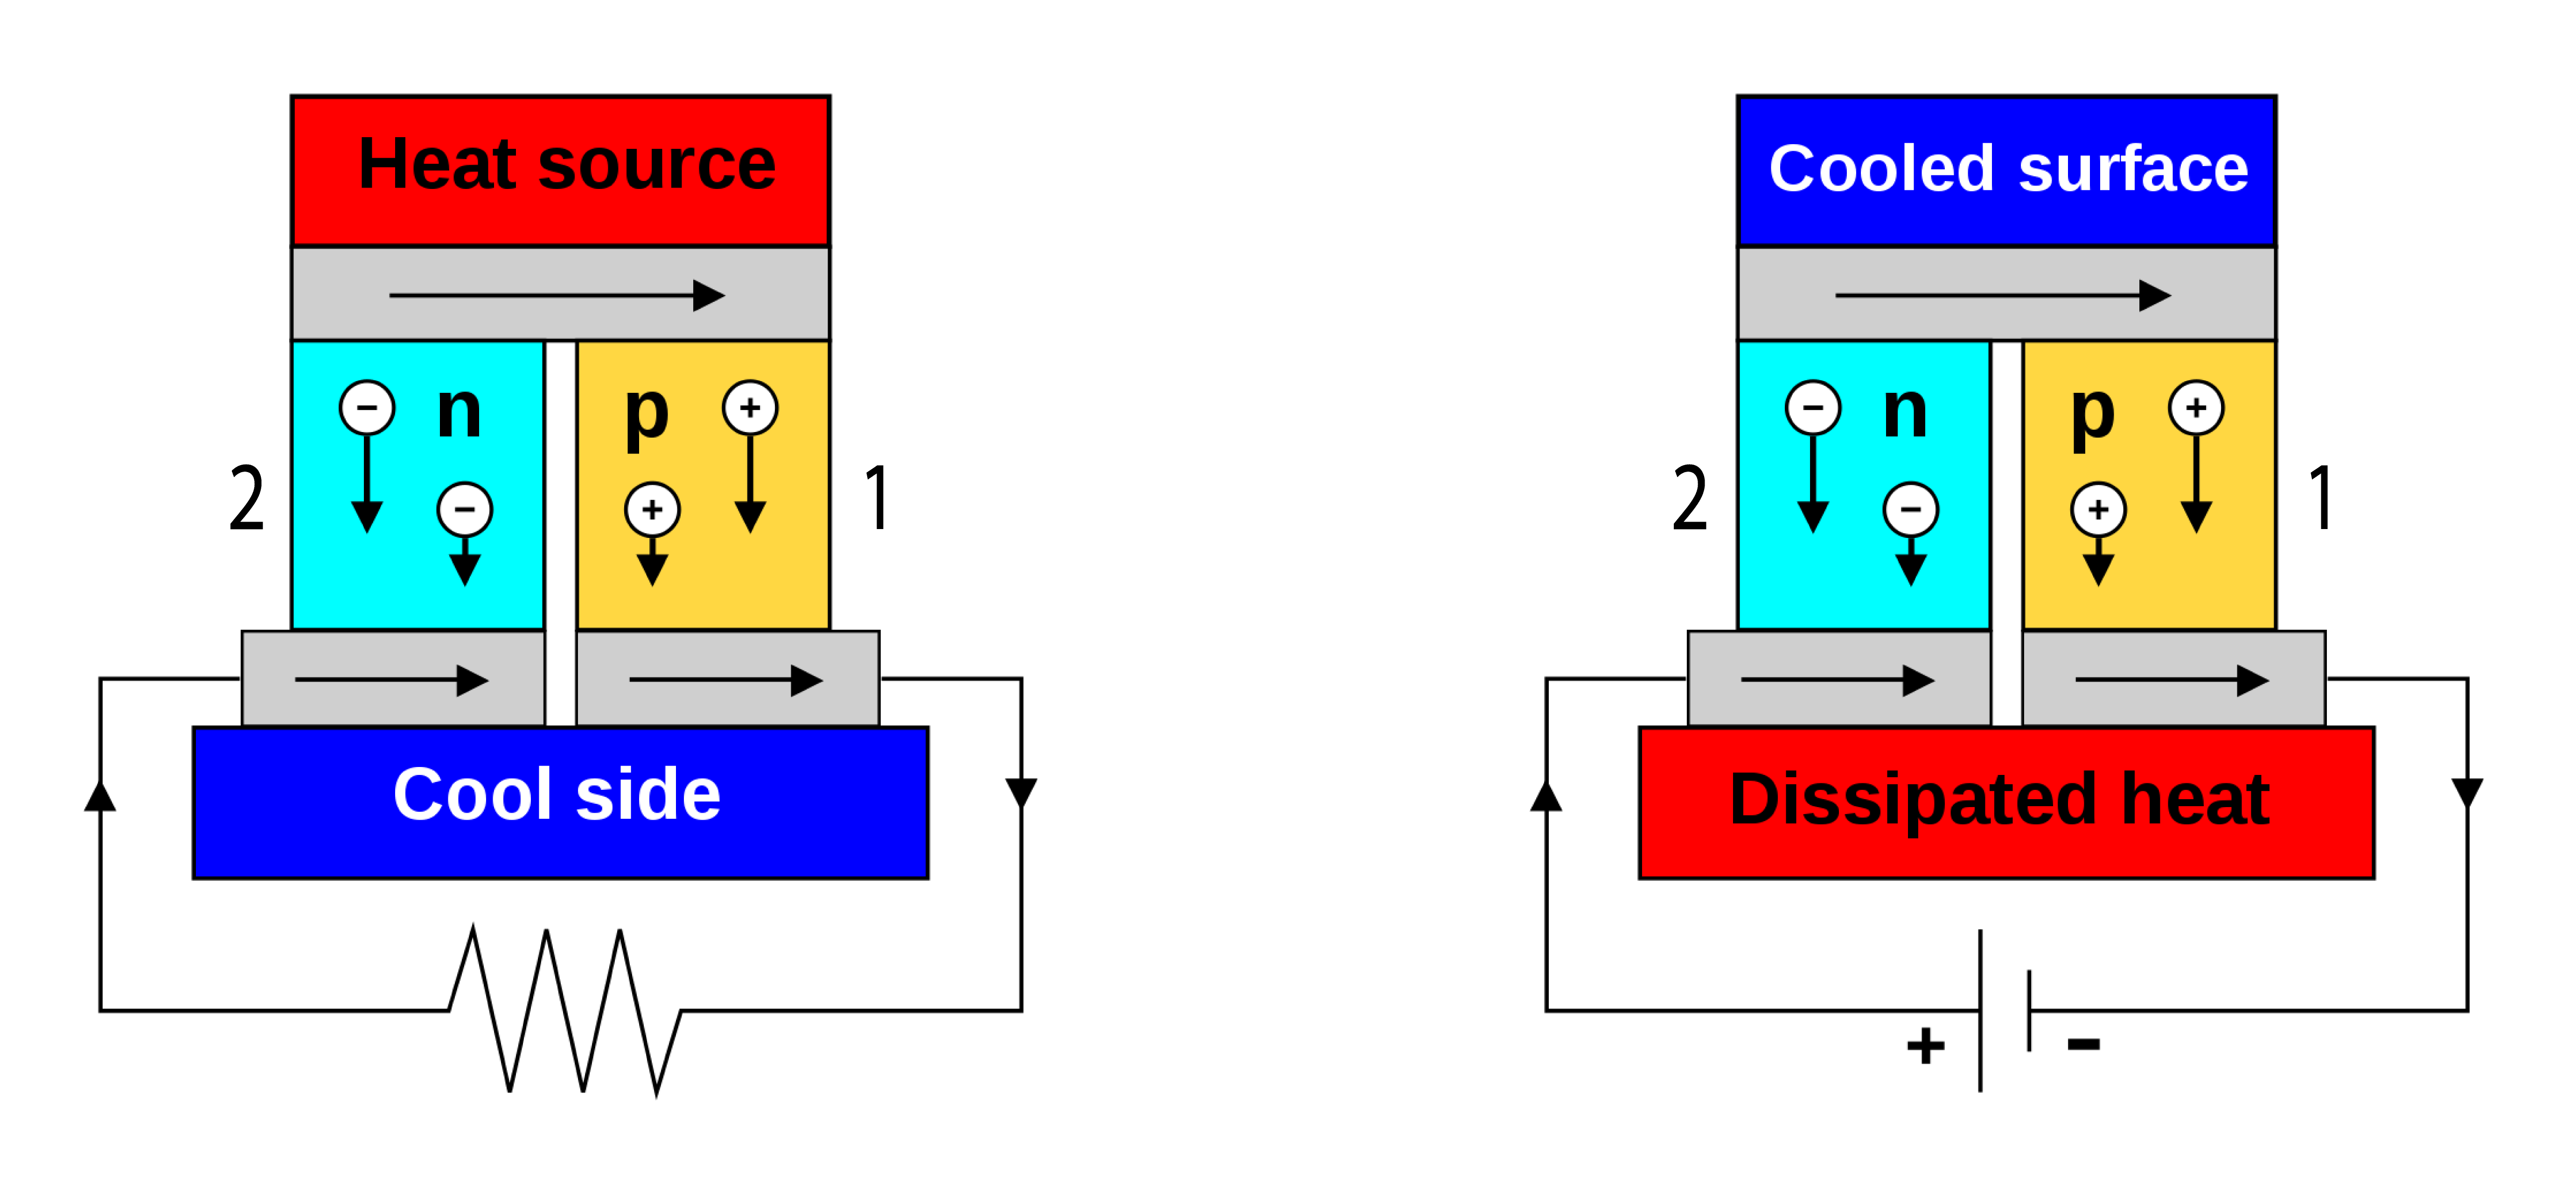
\includegraphics[width=13cm]{image/5-2-21.png}
\caption{Seebeck效应与Peltier效应}\label{fig5-2-21}
\end{figure}

\subsubsection{\hei 佩尔捷({\it Peltier\,})效应}
类似于索瑞效应与杜福尔效应的关系,\,温差可以耦合电流,\,那么这个效应也会反过来对热传导造成影响.\,第一个效应是佩尔捷效应,\,当电流\(I\)以其正向流过以上连接点处时,\,连接点会产生一部分独立于热传导外的吸放热.\,这个热量被称为佩尔捷热,\,以电流从\(1\)到\(2\)为正,\,热量产生为正,\,则经验公式为:
\[\dot{Q}=(\pi_1-\pi_2)I\]

其中\(\pi_i\)为材料\(i\)的佩尔捷系数.

\subsubsection{\hei 汤姆孙({\it Thomson\,})效应}
汤姆孙也就是开尔文爵士,\,他在1851年前后系统地研究了热电耦合的两个效应,\,并在理论上预言和实验上观测了连续版本的佩尔捷效应---即汤姆孙效应.\,这个效应只需要把上式中的热产生率换成热产生率密度,\,而佩尔捷系数之差理解为某种和温度有关的性质的梯度,\,电流改为电流密度,\,得到:
\[\dot{q}=-k\bs{J}\cdot\nabla T\]

这样一些线性现象可以代表在统计力学方法出现前人们对近平衡态研究成果.

\subsection{传热的熵产生}
我们先建立简单的热传导过程的热力学理论.\,在热传导的过程中每一处的熵增都是由于左右两侧的传热造成的,\,根据热力学第一定律,\,单位体积内的内能增加为:
\[\frac{\partial u}{\partial t}=-\nabla\cdot\bs{J}_q\]

而凡是内能增加即体现为熵增:
\[\delta u=\delta q=T\delta s\]

那么熵的等式可以化为:
\[\frac{\partial s}{\partial t}=-\frac{1}{T}\nabla\cdot\bs{J}_q\]

至此已足够明显,\,如果定义\emph{熵流}(entropy flow),\,它由其他流共同体现,\,在热传导时热流即也携带熵流:
\[\bs{J}_s=\frac{\bs{J}_q}{T}\]

那么熵流本身不能完全反应每一点处熵的增加,\,还要引入\emph{熵产生}(entropy production)的概念,\,比如在此种情形下为:
\[\theta=\bs{J}_q\cdot\nabla\frac{1}{T}\]

那么有以下熵连续性方程:
\[\frac{\partial s}{\partial t}=-\nabla\cdot\bs{J}_s+\theta\]

\subsection{普遍理论与昂萨格倒易关系}
一般来讲,\,熵密度的改变往往与体积内的某种``荷''\(q_\alpha\)与``势''\(f_\alpha\)有关,\,一般可以表示为:
\[\delta s=\sum_\alpha f_\alpha \delta q_\alpha\]

而每一种``荷''都有其连续性方程:
\[\frac{\partial q_\alpha}{\partial t}=-\nabla\cdot \bs{J}_\alpha\]

从而一样地我们写出:
\[\frac{\partial s}{\partial t}=-\nabla\cdot\bs{J}_s+\theta\]
\[\bs{J}_s=\sum_\alpha f_\alpha \bs{J}_\alpha\quad ;\quad \theta=\sum_\alpha \bs{J}_\alpha\cdot\nabla f_\alpha\]

从而流就是\(\bs{J}_\alpha\)而力就是\(F_\alpha=\nabla f_\alpha\),\,那么近平衡区的线性输运特性可以表示为:
\[\bs{J}_\alpha=\sum_\beta L_{\alpha\beta}\nabla f_\beta\]

中间的经验系数构成的矩阵就是\emph{昂萨格矩阵}(Onsager matrix).\,通过对微观过程可逆性的研究,\,昂萨格断言:
\[L_{\alpha\beta}=L_{\beta\alpha}\]

即这个矩阵是一个对称的(半正定)矩阵,\,任意两种流与力之间的交叉耦合强度实际上应该相等.\,这就是\emph{昂萨格倒易关系}(Onsager reciprocal relation),\,由于其普适性,\,它经常被当成热力学第四定律\footnote{本书将不涉及热力学第三定律}.\,从而整体熵产生被表示为一个二次型:
\[\theta=\sum_{\alpha\beta} L_{\alpha\beta}\nabla f_\alpha\cdot\nabla f_\beta\]

\subsection{推证热电耦合的普遍规律}
热电耦合问题中存在两种流,\,一是热流\(\bs{J}_q\),\,定义为单位面积单位时间内通过的热量.\,二是电流\(\bs{J}_p\),\,我们命载流子为正电荷,\,电量为\(p\),\,而把化学势约化为单位电荷的:\,\(\zeta=\mu/p\)则\(\mu n\)项变为\(\zeta\rho\).\,\(\rho\)为电荷密度.\,在导体导电问题中有一些不同于普遍理论之处:\,一是有外电场的存在,\,它会对流做功而直接导致输运,\,二是化学势的变化一般可以忽略,\,而仅在两种导体接触处才需要考虑.\,我们写出此时的内能连续方程:
\[\frac{\partial u}{\partial t}=-\nabla\cdot\bs{J}_q-\nabla\cdot(\zeta \bs{J}_p)-\bs{J}_p\cdot\nabla\varphi\]

第一项是传热输入的能量,\,第二项是传入粒子所带来的能量,\,第三项还有外电场\(\bs{E}=-\nabla\varphi\)对电流所做的功.\,而电荷连续方程写为:
\[\frac{\partial \rho}{\partial t}=-\nabla\cdot\bs{J}_p\]

熵的大小为:
\[\delta s=\frac{1}{T}\delta u-\frac{\zeta}{T}\delta \rho\]

代入化简得:
\begin{align*}
\frac{\partial s}{\partial t}	&=-\frac{1}{T}\nabla\cdot \bs{J}_q-\frac{1}{T}\bs{J}_p\cdot\nabla(\zeta+\varphi) \\
								&=-\nabla\cdot(\frac{1}{T}\bs{J}_q)+[\bs{J}_q+(\zeta+\varphi)\bs{J}_p]\cdot\nabla\frac{1}{T}-\bs{J}_p\cdot\nabla\frac{\zeta+\varphi}{T} \\
								&=-\nabla\cdot(f_1\bs{J}_1+f_2\bs{J}_2)+\bs{J}_1\cdot\nabla f_1+\bs{J}_2\cdot\nabla f_2 \\
								&=-\nabla\cdot\bs{J}_s+\theta
\end{align*}

其中第一个流是能量量纲的\(\bs{J}_1=\bs{J}_q+(\zeta+\varphi)\bs{J}_p\),\,对应的``势''为\(f_1=1/T\);\,第二个流是电荷量纲的\(\bs{J}_1=\bs{J}_p\),\,对应的``势''为温度约化的电化学势\(f_2=-(\zeta+\varphi)/T\).\,这样我们写出昂萨格线性关系:
\[\begin{matrix}
\bs{J}_q+(\zeta+\varphi)\bs{J}_p & = & L_1\nabla\dfrac{1}{T} & - & M\nabla\dfrac{\zeta+\varphi}{T} \\[5pt]
\bs{J}_p & = & M\nabla\dfrac{1}{T} & - & L_2\nabla\dfrac{\zeta+\varphi}{T}
\end{matrix}\]

对应欧姆定律,\,命上式温度梯度为零,\,在一种导体中\(\zeta\)始终认为是一个常数,\,有:
\[L_2=\sigma T\]

而对应温差电效应,\,我们消除外电场,\,让\(\varphi\)是一个常数,\,用塞贝克系数可以确定\(M\):
\[M=\sigma T(\eta T+\zeta+\varphi)\]

最后再由傅里叶定律,\,让电流\(\bs{J}_p\)为零,\,得到:
\[L_1=\kappa T^2+\sigma T(\eta T+\zeta+\varphi)^2\]

最后整理得:
\[\begin{matrix}
\bs{J}_q & = & -(\kappa +\sigma\eta^2 T)\nabla T & - & \sigma\eta T\nabla(\zeta+\varphi) \\
\bs{J}_p & = & -\sigma\eta\nabla T & - & \sigma\nabla(\zeta+\varphi)
\end{matrix}\]

首先考虑伽伐尼接触电势差,\,显然当且仅当上式中两个梯度为零时所有流都将消失.\,从而相互接触的两种介质有
\[\zeta_1+\varphi_1=\zeta_2+\varphi_2\quad\Longrightarrow \varphi_1-\varphi_2=-\frac{1}{p}(\mu_1-\mu_2)\]

如果是金属\(p=-e\)我们便得到了之前熟知的结果.\,再考虑佩尔捷效应,\,我们依然认为两介质满足以上式子,\,这是因为此时由\(\nabla\varphi\)驱动的电流应该认为是发生在两种介质中,\,而分界面上仍是这个固定的接触电势差.\,那么对于电流从介质\(1\)流向\(2\)的情况,\,再命上式中温度均匀不变,\,有:
\[\bs{J}_{q,i}=\eta_i T\bs{J}_{p,i}\]

也就是说电流恰好携带着一个热流.\,由内能连续性:
\[\dot{Q}=\frac{\ud U}{\ud t}=\eta_1 TI-\eta_2 TI+(\zeta_1+\varphi_1)I-(\zeta_2+\varphi_2)I\]
后两项表示输入输出的电流粒子带来的能量与电场力的做功,\,这两项恰好消掉了.\,于是得到了佩尔捷效应的公式,\,并发现佩尔捷系数实际上就是:
\[\pi=\eta T\]

这是开尔文爵士当年得出的两个关系之一,\,称之为\emph{第二汤姆孙关系}(the second Thomson relation).\,我们再研究连续情形的内能连续性,\,再次使用之前的表达式:
\[\frac{\partial u}{\partial t}=-\nabla\cdot\bs{J}_q-\nabla\cdot(\zeta \bs{J}_p)-\bs{J}_p\cdot\nabla\varphi\]

首先根据昂萨格关系,\,注意到任意情况下都有:
\[\bs{J}_q=\eta T\bs{J}_p-\kappa\nabla T\]

再注意到在我们要研究的问题中电流仍连续:
\[\nabla\cdot  \bs{J}_p=0\]

代入上式,\,通过昂萨格关系化简便得:
\[\dot{q}=\nabla\cdot(\kappa\nabla T)+\frac{\bs{J}_p^2}{\sigma}-T\bs{J}_p\cdot\nabla\eta\]

上式第一项表示热传导积累的热,\,第二项是焦耳热,\,第三项就是汤姆孙热了.\,可见它是由于塞贝克系数\(\eta\)不均匀而导致的,\,一般就是其与温度有关\footnote{既然\(\eta\)可以随温度改变,\,那么\(\kappa\)随温度的改变其实也应考虑在内.\,当然这一项是纯导热现象而与电流没有耦合.},\,温度梯度也造成了一个塞贝克系数的梯度\(\nabla\eta=\dfrac{\ud \eta}{\ud T}\nabla T\),\,从而我们也得到了开尔文系数:
\[k=T\frac{\ud \eta}{\ud T}=\frac{\ud \pi}{\ud T}-\frac{\pi}{T}\]

上式即被称作\emph{第一汤姆孙关系}(the first Thomson relation).

这就是近平衡态线性热力学理论对热电耦合现象的解释大意.
%!TEX root = ../physical-olympics-2.tex
\chapter{液体与固体的性质}

在讲解热力学基本规律的过程中,\,我们已经对气体,\,尤其是理想气体这样的热力学体系有了一定的了解.\,但是对于与我们的生活息息相关的\emph{液体}(liquid)与\emph{固体}(solid)两种\emph{凝聚态}(condensed matter)我们还知之甚少.\,在此稍作一步展开介绍.

\section{固体晶格论}

\subsection{经典晶格论}

\begin{wrapfigure}[8]{o}[-10pt]{7cm}
\centering
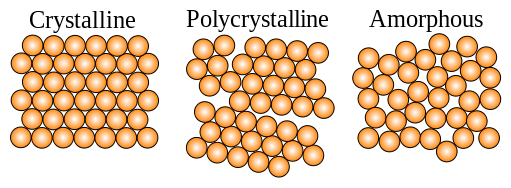
\includegraphics[width=7cm]{image/5-3-2.png}
\caption{单晶体,\,多晶体与无定形体}\label{fig:3crystal}
\end{wrapfigure}
固体在此处实际上特指\emph{晶体}(crystal).\,晶体应具有\emph{长程序}(long-ranged order),\,也就是说组成的晶体的原子,\,分子,\,或者离子应体现出大范围的空间周期性.\,如图\ref{fig:3crystal}所示,\,一整块物质如果完全由严格的周期性结构组成,\,那么一般其表面也是规则的几何形状,\,称作\emph{单晶体}(single crystal).\,但是即使单晶体内部是充满着\emph{缺陷}(defect)的,\,无论是原子的\emph{缺失}(vacancy)还是\emph{填隙}(interstitial),\,还是更复杂的面缺陷与体缺陷,\,都会使得晶体的不同区域变得孤立起来,\,常见的金属,\,冰,\,陶土,\,岩石都是由大量可视作晶体的晶粒拼接而成,\,在物理性质上丧失了单晶体所具有的的各向异性而成为\emph{多晶体}(polycrystal).\,最后还有丧失了长程序的\emph{无定形体}(amorphous solid),\,又做非晶体,\,玻璃体.\,比如玻璃,\,蜡,\,塑料等,\,它们都不是晶体,\,但一般仍认为是固体.

固体的结合方式在极大程度上决定了其热学性质,\,而固体的结合又在很大程度上依赖于其外层的电子在量子统计规律下的诸多行为.\,根据最后的结果我们可以粗浅地分类:
\begin{figure}[H]
\centering
\begin{tabular}{c|c}
\hline
晶体类型			&		结合方式\\ \hline\hline
原子晶体			& 局域在原子间的共用价电子对与原子实之间的相互吸引 \\ \hline
离子晶体 		& 一种原子的电子几乎完全被另一种原子剥夺形成离子,\,两种离子相互吸引 \\ \hline
金属晶体			& 非局域的共享电子们与原子实们之间的相互吸引 \\ \hline
分子晶体 		& 分子与分子之间十分微弱的氢键,\,范氏相互吸引,\,还包含电偶极矩磁偶极矩相互作用 \\ \hline
\end{tabular}
\end{figure}


在某些较为简单的情形下,\,我们会认为固体可以拆解为两个体系,\,一是由\emph{原子实}(atomic core)构成的\emph{点阵}(lattice),\,一是参与原子间相互作用的所有\emph{价电子}(valance electron)构成的\emph{电子气}(electron gas).\,后者是那么地轻盈,\,但是却带有与原子实等量反号的电荷,\,这一点造成了如下的局面:\,体系的动能几乎由具有绝大多数质量的点阵承担\footnote{其实这也是个量子效应,\,详见之后章节.};\,而势能也由点阵的位置与变形来计算,\,对于电子的分布,\,总是遵循泡利不相容原理和最小势能原理,\,故可由点阵位置计算.\,这种\emph{平均场论}(mean field theory)的思想使我们写出体系的总能量来:
\[H=\sum_g T(\bs{v}_{i,g})+V(\bs{r}_{i,g})\quad ,\quad i=1,2\cdots n\;;\;g\in G\]

\begin{wrapfigure}[13]{o}[-10pt]{6cm}
\centering
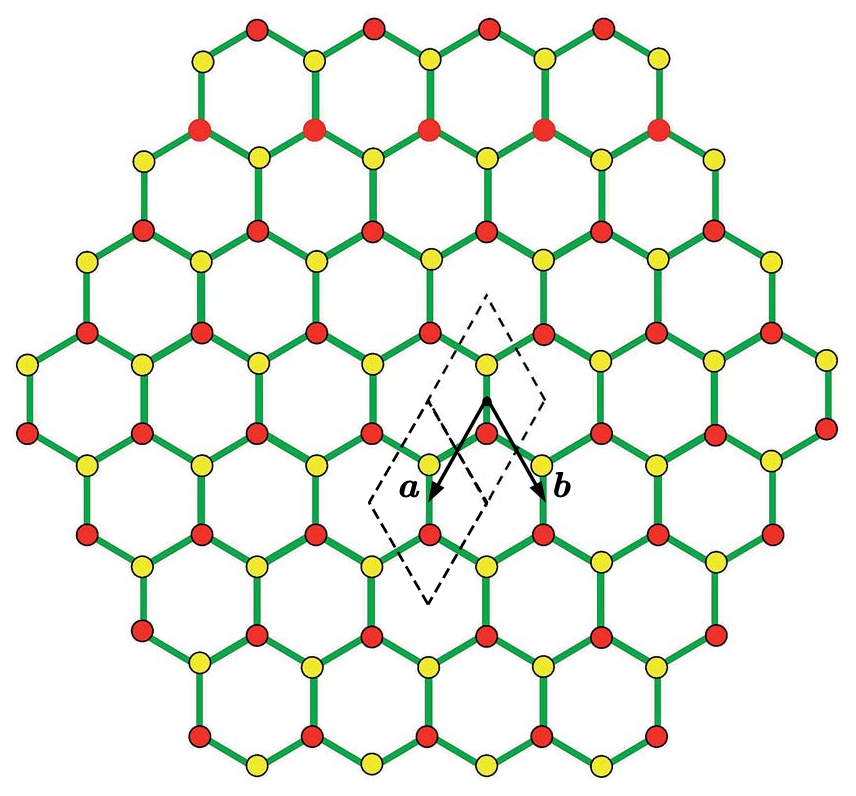
\includegraphics[width=6cm]{image/5-3-4.png}
\caption{石墨烯的结构}\label{fig:graphene}
\end{wrapfigure}
式中$G$表示所有\emph{原胞}(unit cell)的集合,\,将一个原胞按照$G$的方式平移便得到了整个晶体,\,称作\emph{布拉伐格子}(Bravais lattice).\,而每一个原胞都是全同的,\,内含$1,2\cdots n$号原子.\,以\emph{石墨烯}(graphene)为例,\,\emph{石墨}(graphite)实际上即由一层一层的石墨烯通过范德瓦尔斯力吸引而形成.\,每一层可以认为是一种平面型的原子晶体.\,其原胞由两个并不具有平移等价性的原子构成.\,原胞形状为菱形,\,故可以在$x-y$平面上按密铺,\,具有平移对称性,\,如果我们把沿两个$x-y$平面上独立方向的对称平移矢量$\bs{a},\,\bs{b}$找到,\,那么所有平移对称性就能够被记做:
\[G=\{p\bs{a}+q\bs{b}|p,\,q\in  \mathbb{Z}\}\]

从而能量的一种最简单的写法就是:
\[H=\sum_{pq}  \frac{1}{2}m(\dot{x}_{1,pq}^2+\dot{y}_{1,pq}^2+\dot{x}_{2,pq}^2+\dot{y}_{2,pq}^2)+\frac{1}{2}k{\color{red}[}(x_{1,pq}-X_{1,pq})^2+(y_{1,pq}-Y_{1,pq})^2\]
\[\qquad +(x_{2,pq}-X_{2,pq})^2+(y_{2,pq}-Y_{2,pq})^2{\color{red}]}+\frac{1}{2}m'(\dot{z}_{1,pq}^2+\dot{z}_{2,pq}^2)+\frac{1}{2}k'(z_{1,pq}^2+z_{2,pq}^2)\]

上式$1$表示上图中每一个原胞中的黄色原子的动能和势能,\,$2$则表示红色原子的能量.\,这背后的原理是,\,首先动能自然是正比于速度的平方的,\,而势能在平衡位置$(X_{i,pq},\,Y_{i,pq},\,0)$附近泰勒展开也至少是从二阶项开始.\,由于只考虑原子偏离平衡位置不多的情况,\,所以只保留最低阶的项.\,所以都是二次型.\,由于红色黄色原子在中心反演下对称,\,故两者系数$m,\,k$也是相等的.\,而在平面上的能量具有三重旋转对称性,\,具有这样的对称性的二次型只能在所有方向上都具有相同的系数,\,故连$x,\,y$的系数都是一样的.\,但是$z$方向的运动则可以具有不一样的系数$m',\,k'$.

这样极端的近似存在一个致命的缺陷: 忽略了格点与格点之间的相互作用, 下文我们将采取一种弹性原子链模型来弥补这个缺陷. 但这个处理足以带来第一个关键的信息:\,我们发现上面一共具有$12$个平方项,\,这就是说,\,根据之前说过的,\,之后还将讨论的能均分定理,\,该单元的总平均能量为:
\[\varepsilon_{\rm cell}=\frac{1}{2}kT\cdot 12=6kT\]

或者说对于这样的原子晶体(离子晶体,\,金属晶体也是类似的),\,其每一个原子上的平均能量就是:
\[\varepsilon=3kT\]

这其实是一个普遍的性质,\,任何原胞里面如果具有$n$个原子,\,那么对应的动能项和势能项就会各有$3n$个,\,相当于每个原子平均具有三个动能项和势能项,\,对应三个运动的维度.\,从而平均能量就是$3kT$.\,那么整个晶体的总内能就是:
\[U=3NkT=3\nu RT\]

即晶体的摩尔热容是:
\[C_{m}=3R\]

这是\emph{杜隆-裴替定律}(Dulong-Petit law).\,有四点值得注意:

1.\,以上摩尔热容指的是每一摩尔原子的热容.\,例如NaCl晶体,\,每一摩尔的NaCl应当按$2$摩尔原子计算.

2.\,以上内能只计算了振动导致的热运动形式的能量.\,晶格自己的结合能自然也是内能的一部分,\,被我们直接处理为不变的常数而从``有效''内能中略去了.\,如果考虑热膨胀甚至晶格的解离,\,如熔化或溶解的过程,\,显然这个过程内能的改变就会用到这一部分.\,另,\,对于固体来说等体热容和等压热容的差别很小可以忽略不计,\,因为固体温度不同的体积膨胀与气体相比实在太细微.

3.\,电子对热容的贡献被忽略了,\,这个做法甚至是合理的.\,背后有一定的量子力学原理:\,电子被量子效应束缚在定态上:\,它们要么是束缚电子处于原子轨道中,\,要么是价电子处于分子轨道上,\,甚至金属中的自由电子也其实是在一定的能带结构中,\,本质上还是被所有原子实束缚.\,故计算表明室温下这些电子产生的热容是可以忽略不计的.\,在室温下,\,即使是金属,\,它们的热容与杜隆-裴替定律符合地也是相当地好的.\,但是在较高的\emph{费米温度}(Fermi temperature)量级开始,\,其热容明显大于$3R$.\,量级基本上在几万开尔文.\,这个温度下基本上物质也称为等离子体态而不是固态了.

4.\,最后,\,晶格热容低温下杜隆-裴替定律也会失效.\,也是与量子效应有关.\,典型的温度称作\emph{德拜温度}(Debye temperature).\,明显低于德拜温度时晶格热容将迅速减小.\,常见金属的德拜温度在室温附近,\,而非金属单质的德拜温度往往较低.\,如果温度特别低,\,那么可以证明晶格的热容将正比于温度的$3$次方,\,而电子造成的热容将正比于温度的$1$次方.\,之后我们会做简要讨论.

\begin{figure}[H]
\centering
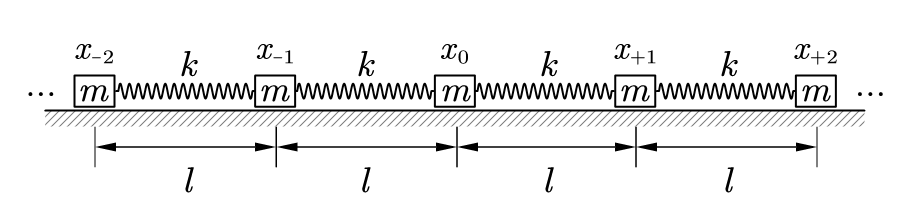
\includegraphics[width=15cm]{image/5-3-5.png}
\caption{弹性}
\end{figure}

认为固体单元之间有十分简单的平方形式的弹性势能,\,这是近似但实用的.\,正如\emph{弹性}(elasticity)的概念正发源于其中,\,在简化的一维原子链模型下,\,正如力学的弹性体中所描述的那样,\,这样一个体系就会产生弹性.\,其纵向的弹性模量为:
\[F=K\frac{\Delta L}{L}\quad \Rightarrow \quad K=kl\]

那么沿三维晶体的一条原子链方向的拉伸压缩形变的杨氏模量,\,就可以不严谨地认为是以上的$K$除以每一条原子链``占据''的截面积.\,但是这个模型有一个缺点:\,温度升高以后原子仅仅是围绕既定的平衡位置做热振动,\,从而就无法产生正常固体具有的\emph{热膨胀}(thermal expansion)现象.

为了解释热膨胀现象我们就需要对既定的模型进行适度的扩充.\,其实热膨胀可以简单地来自于其相互作用的\emph{非谐性}(anharmonicity).\,简谐的受力是线性回复的,\,简谐的势能是至多二次的多项式的形式,\,势能函数的图像是标准的抛物线.\,但是只要在势能函数中最小增添一个三次项,\,就可以导致势能的非谐性.\,对于任意非线性力的势能函数组成的一维原子链,\,热膨胀其实就来自这个势能的非零三阶导数.\,例如,\,我们依然认为一维原子链中,\,只有相邻的两个原子之间才有相互作用,\,例如形式为\emph{李纳-琼斯势能}(Lennard-Jones potential)\footnote{然而这个势能适用于不带电,\,无偶极矩,\,不成化学键的两个原子或分子之间的作用力.\,其他的力一般更强而具有更低的幂次.}:
\[V(u)=V_0  \left[ -2\left( \frac{u_0}{u} \right)^6+ \left( \frac{u_0}{u} \right)^{12}\right]  \]

这样在平衡的时候(无热振动),\,相邻原子之间的距离为$l=u_0$.\,即势能曲线的最低点对应的距离.\,在该点处,\,该势能的二阶展开给出了这个模型对应的简谐模型中的劲度系数$k$:
\[V=V(u_0)+\frac{1}{2}V''(u_0)(u-u_0)^2 \quad,\quad k=V''(u_0)=72\frac{V_0}{u_0^2}\]

现在$u-u_0$表示的是两个质点的间距.\,现在用$x$表示它,\,如果势能仅仅是上式给出的:
\[V=-V_0+\frac{1}{2}kx^2\]

这样的势能就不会产生热膨胀的效果,\,经典物理的观点是,\,如果体系以一定形式在这样一个势能平衡位置处振动,\,往左往右位移的幅度和停留时间都是对称的,\,那么平均起来相当于两原子平均距离没有改变.\,其实更精确的观点应当是:\,其原子间的距离应当满足一个玻尔兹曼分布.\,现在让我们考虑泰勒展开的三阶项:
\[V'''(u_0)=-1512\frac{V_0}{u_0^3}\]

即势能变为:
\[V=-V_0+\frac{1}{2}kx^2+\frac{V'''(u_0)}{6}x^3=-V_0+cx^2-gx^3 \quad,\quad g=252\frac{V_0}{u_0^3}\]

根据玻尔兹曼分布理论,\,分子之间的平均距离对应的$x$的计算公式应当是:
\[\langle x\rangle=\frac{\int xe^{-V/k_{\rm B}T}\ud x}{\int e^{-V/k_{\rm B}T}\ud x}\]

在计算中做如下近似:
\[e^{gx^3/kT}\approx1+\frac{gx^3}{k_{\rm B}T}\]

得到以上积分为:
\[\langle x\rangle=\frac{\frac{3\pi^{1/2}(k_{\rm B}T)^{3/2}g}{4c^{5/2}}}{\frac{\pi^{1/2}(k_{\rm B}T)^{1/2}}{c^{1/2}}}=\frac{3g}{4c^2}k_{\rm B}T\]

这就可以给出\emph{热膨胀系数}(thermal expansion coefficient)的值:
\[\frac{\Delta L}{L}=\alpha T \quad\Rightarrow \quad \alpha=	\frac{3k_{\rm B}g}{4u_0c^2}\]

这个热膨胀系数实际上是线膨胀系数,\,体膨胀系数,\,由小量近似方法容易得到,\,应是线膨胀系数的三倍.\,在温度变化范围不大的情况下,\,这两个系数根据公式都是常数,\,所以固体的长度和体积分别按照以下公式变化:
\[\alpha_V=3\alpha_L=3\alpha\]
\[L=L_0(1+\alpha T)\quad,\quad V=V_0(1+\alpha T)\]

其中$L_0,\,V_0$为假想的外推到绝对零度时的原长,\,原体积.

类似于热容的性质,\,把简谐的势能改为非谐的情况下,\,尽管产生了一个热膨胀系数,\,但是它其实完全是个常数.\,在温度较低的情况下,\,热容的杜隆-裴替定律和线膨胀系数的上理论公式将会同时失效.


\subsection{量子晶格论*}

此前在力学中我们讨论过两个模型:

一是连续介质的弹性波模型. 在一个杨氏模量为$E$的密度为$\rho$的无限长的自由棒\footnote{我们也说过, 如果是连续的三维介质, 一个波矢$\bs{\kappa}$下就存在更复杂的三个振动模式, 纵波与其平行, 横波与其垂直. 其波速依赖于材料剪变模量$G$和体弹性模量$K$:
\[v_P=\sqrt{\frac{K+4G/3}{\rho}}\quad ,\quad v_S=\sqrt{\frac{G}{\rho}}\]}的弹性运动模式中, 值得注意的是以下基础的行波解:
\[\xi(t)=A\cos(\omega t-\kappa x+\varphi)\quad ,\quad \frac{\omega}{\kappa}=\sqrt{\frac{E}{\rho}}\]

二是考虑宏观物质实际上是由离散的单元所构成的格波模型. 我们也得到了以下行波解:
\[x_n(t)=A\cos(\omega t-n\kappa l+\varphi)\quad ,\quad \omega^2=\frac{4k}{m}\sin^2\frac{\kappa l}{2}\]

在两个问题中, $\omega,\,\kappa$都是满足色散关系下可连续取值的. 而研究本征模式可替代研究单个质元或格点的运动, 因为整个体系的运动除了看做所有单个质元或格点的运动的组合, 也可以分解为本征模式的叠加:
\[x_n(0)=\int_{-\pi/l}^{\pi/l} [A(\kappa)\cos n\kappa l+B(\kappa)\sin n\kappa l]\ud \kappa\]

上式其实是一种\emph{离散傅里叶变换}(discrete fourier transform, DFT)\footnote{更准确的来讲是DTFT}, 这一点在接下来的分析中将会变得明了. 其中$\kappa$的取值范围在\emph{第一布里渊区}(first Brillouin zone):
\[-\frac{\pi}{l}<\kappa\leq \frac{\pi}{l}\]

这是因为$\kappa+j\cdot 2\pi/l$与$\kappa$对应的两种振动模式没有任何区别: 相邻两个格点振动的相位差只是多了$2\pi$的整数倍.

出于三个考虑: a. 以上离散傅里叶变换的$A(\kappa),\,B(\kappa)$算法并不直观. b. 真实热学体系并不是无限长原子链, 而是具有粒子数$N$. c. 虽然真实热学体系总是存在复杂的边界条件, 但是在远离边界的区域选取一个粒子数为$N$的子系统时, 边界与内部变得没有区别. 综合考虑我们重新建立一个类似于格波模型的有限原子链模型:

\begin{figure}[H]
\centering
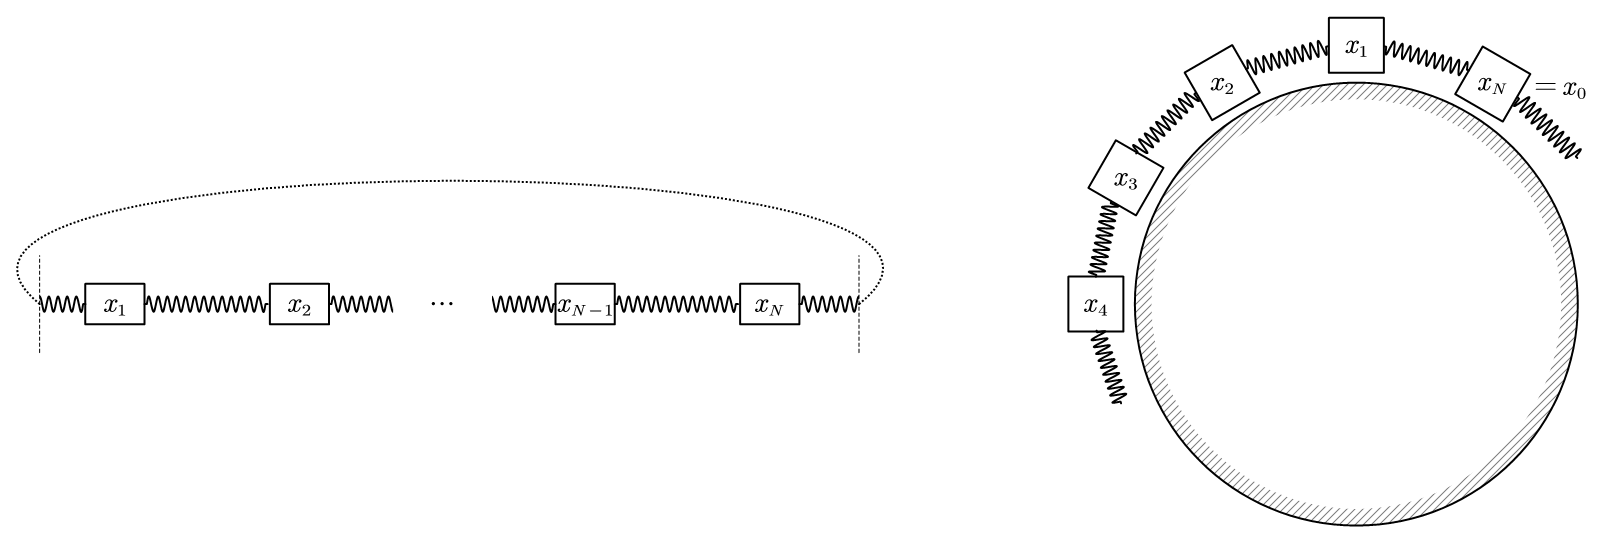
\includegraphics[width=16cm]{image/5-3-7.png}
\caption{周期性边界条件}
\end{figure}

如上图左, $N$个原子排成链状. 并给予其周期性边界条件:
\[x_0=x_N\]

物理上可以理解为这$N$个原子绕成了环状. 如果$N$很大, 这样的体系就能反应一般的热学链条内部的性质. 在这个条件下, $\kappa$的取值就变得有限:
\[N\kappa l=j\cdot 2\pi\quad j=1,\,2,\,3\cdots N\]

故总共只有$N$种可能的振动模式, 第$j$种模式下:
\[x_n(t)=A_j\cos(\omega_j t-n\kappa_j l+\varphi)\quad ,\quad \omega_j^2=\frac{4k}{m}\sin^2\frac{\kappa l}{2}\]

为了使得推导更简洁, 引入复数表示法. 将以上模式叠加计算系数:
\[x_n(0)=\sum_{j=1}^N A_j e^{-2\pi\ui\frac{nj}{N} }\]

十分关键的一点是, 我们不是单纯把上式看做零时刻的坐标确定每一种模式的强度系数$A_j$的决定式. 而是直接看做一种任意时刻都恒成立的坐标变换:
\[x_n=\sum_{j=1}^N q_j e^{-2\pi\ui\frac{nj}{N}}\]

这个变换就是真正意义上的离散傅里叶变换. 它的逆变换与通常的傅里叶逆变换形式类似. 只需要计算:
\[\sum_{n=1}^N x_n e^{2\pi\ui\frac{nj'}{N}}=\sum_{n=1}^N\sum_{j=1}^N q_j e^{-2\pi\ui\frac{nj}{N}}e^{2\pi\ui\frac{nj'}{N}}=\sum_{j=1}^N\left(\sum_{n=1}^N  e^{2\pi\ui\frac{n(j'-j)}{N}}\right)q_j\]

括号内的求和式在$1\leq j\,j'\leq N$时仅有$j=j'$才不为零, 此时指数函数取$1$求和$N$次. 故:
\[\sum_{n=1}^N x_n e^{2\pi\ui\frac{nj'}{N}}=Nq_{j'}\]

从而得到此前坐标变换的逆变换:
\[q_j=\frac{1}{N}\sum_{n=1}^N x_n e^{2\pi\ui\frac{nj}{N}}\]

这个变换可不止是$q_j(0)$表示体系振动分解为本征模式的一个系数的作用那么简单, 它可以直接改写这个体系的动能和势能函数. 首先将动能和势能形式改写成:
\[T=\sum_{n=1}^N \frac{1}{2}m\dot{x}_n^*\dot{x}_n\]
\[V=\sum_{n=1}^N \frac{1}{2}k(x_n^*-x_{n-1}^*)(x_n-x_{n-1})=\frac{1}{2}\sum_{n=1}^N 2k {x}_n^* {x}_n-\frac{1}{2}\sum_{n=1}^N k (x_n^* x_{n-1}+x_{n-1}^* x_{n})\]

代入以上变换并化简得到:
\[T=\frac{1}{2}\sum_{j=1}^N Nm\dot{q}_j^*\dot{q}_j\]
\[V=\frac{1}{2}\sum_{j=1}^N 2Nk\left(1-\cos\frac{2\pi j}{N}\right) {q}_j^* {q}_j=\frac{1}{2}\sum_{j=1}^N 4Nk\sin^2\frac{\pi j}{N} {q}_j^* {q}_j\]

这就可以直接看出. 整个体系变成了$j=1,\,2\cdots N$对应的谐振子的直接合成:
\[H=\sum_{j=1}^N  \frac{1}{2}Nm(|\dot{q}_j|^2+\omega_j^2 |q_j|^2) \quad,\quad \omega_j^2=\frac{4k}{m}\sin^2 \frac{\kappa_j l}{2}\;,\;\kappa_j=\frac{2\pi j}{Nl}\]

所以, 通过命$N\to \infty$. 我们就可以得到此前的无限长原子链方案对应的模式系数与其确定方法:
\[x_n(0)=\int_{-\pi/l}^{\pi/l} [A(\kappa)\cos n\kappa l+B(\kappa)\sin n\kappa l]\ud \kappa\]
\[A(\kappa)=\frac{l}{2\pi}\sum_{n=-\infty}^{+\infty}x_n(0)\cos n\kappa l\quad ;\quad B(\kappa)=\frac{l}{2\pi}\sum_{n=-\infty}^{+\infty}x_n(0)\sin n\kappa l\]

至此更值得我们注意的反而是$N$个粒子组成的满足周期性边界条件的情况. 我们通过坐标变换将初始的粒子坐标代换为$N$个广义坐标$q_j$. 这样体系的能量直接变成了$N$个谐振子项:
\[H=\sum_{j=1}^N  \frac{1}{2}Nm(|\dot{q}_j|^2+\omega_j^2 |q_j|^2)\]

那么容易看出每个谐振子的广义坐标就会随时间做简谐振动:
\[q_j=A_j e^{\ui \omega_j t}+A_j' e^{-\ui \omega_j t}\]

这里的``谐振子'', 已经从经典物理中的谐振子概念迈进了更抽象的层面. 经典物理的谐振子$H=m\dot{q}^2/2+kq^2/2$,\,系数$m,\,k$通常有所指, 而且指向某个具体的物理实体的属性. 比如单摆若视作谐振子, 摆角视作广义坐标$q=\theta$, 则系数$m$指单摆对悬挂点的转动惯量, 而$k$值则是单摆质量, 摆长与重力加速度三者的乘积. 我们这里通过坐标变换得到的$N$个谐振子, 每一个谐振子代表的是\emph{集团行为}(aggregate behavior), 从因果性上看, 任何一个格点的运动将对相邻的格点产生动力学影响, 从而从来都无法看成是独立的振子. 但是分解为广义坐标对应的谐振子后, 振子与振子之间的影响就不再存在了.

基于这一点, 从经典的热学理论就可以判定, $N$个振子上的动能和势能就是体系的内能. 但又由于能均分原理, 这个内能就是:
\[U=N\cdot 2\cdot\frac{1}{2}kT=NkT=\nu RT\]

这里是一维原子链. 如果考虑三维情形, 那么上式就回到了此前提过的杜隆-裴替定律:
\[U=3\nu RT\]

但这个坐标变换处理的意义绝对不仅限于在考虑原子间相互作用的情形下得到了一个与不考虑相互作用而采取平均场论的思想得到的结果一致的结果, 它的下一步是考虑能量尺度较低下的\emph{元激发}(elementary excitation).

我们应当已经知道, 在氢原子的电子能量函数下:
\[H=\frac{\bs{p}^2}{2m}-\frac{e^2}{4\pi \varepsilon_0 r}\]

可以得到其角动量和能量的量子化:
\[L_z=m\hbar\quad ,\quad m=0,\,\pm 1,\,\pm 2\cdots\]
\[E=-\frac{E_0}{n^2}\quad ,\quad n=1,\,2,\,3\cdots\]

其背后的物理规律为某在$\hbar$的尺度下才发挥显著功能的量子定律\footnote{暗示薛定谔方程.}. 那么容易想见, 虽然经典谐振子能量连续. 但是如果考虑量子效应, 一个量子谐振子:
\[H=\frac{1}{2}m(\dot{q}^2+\omega^2 q^2)\quad ,\quad q\text{存在不确定性}\]

只要其振动能量足够小, 就也可以看到其能级的量子化现象. 量子理论的推导给出了一个非常简洁的公式\footnote{思考: 如果用相空间面积量子化是否可以得到相同的结果?}:
\[E_n=\left(n+\frac{1}{2}\right)\hbar \omega\]

这就是说, 谐振子的振动幅度不是连续的而是离散的\footnote{准确的说法是振动幅度是不确定的, 但造成了离散的能级}, 不同的振动幅度之间只能以一份一份的形式叠加运动剧烈程度, 每一份叠加的能量子我们就称作元激发:
\[E=\hbar\omega\]

在原子链中的元激发更值得留意, 它是集团模式的元激发, 每一份元激发代表了某种在总质量$M$,\,总长$L$的$N$原子链中传播的行波. 而且由于:
\[H=\sum_{j=1}^N H_j\quad ,\quad H_j=\frac{1}{2}M(|\dot{q}_j|^2+\omega_j^2 |q_j|^2)\;,\; \kappa_j=\frac{2\pi j}{L}\]

故这样的元激发一共有$N$种. 每一种都具有具体的波矢$\kappa_j$与角频率$\omega_j$. 引人注意的是, 如果计算元激发的总动量, 不难发现:
\[p_j=\hbar \kappa_j\]

单个元激发具有动量和能量, 就好像水面上的一朵浪花, 给人以类似移动的物体的直觉, 当然真正在运动的是造成元激发的物质粒子. 但是固体中物质粒子却不能像元激发那样长途迁徙. 能否把单个元激发也形式地视作某种粒子? 这种观点其实是被物理学普遍采用的. 这样的粒子称作\emph{准粒子}(quasiparticle). 它的含义是量子化的集团运动模式:
\[E=\hbar\omega\quad ,\quad \bs{p}=\hbar\bs{\kappa}\]

对于波来说, 一个重要的结论为, 如果考虑波包的运动, 其中心速度应为群速度:
\[v_g=\frac{\ud \omega}{\ud \kappa}\]

这个式子即色散关系, 它在量子理论下将具有更加直白的含义. 我们考虑一个向前以$v_g$传播的波包, 并把它看做元激发或若干元激发的相干态. 那么作为准粒子, 根据元激发具有的能量动量公式, 比较不同$\omega,\,\kappa$的准粒子就有:
\[v_g=\frac{\ud E}{\ud p}\]

甚至可以写为矢量式:
\[\ud E=\bs{v}_g\cdot \ud \bs{p}\]

如何理解这个式子? 设想在准粒子上作用一个力$\bs{F}$, 时间为$\ud t$. 那么力为准粒子带来的动量和动能改变就分别可以参考经典的动量定律和动能定律:
\[\ud\bs{p}=\bs{F}\ud t\]
\[\ud E=\bs{F}\cdot \bs{v}_g\ud t\]

上式代入下式就可以得到:
\[\ud E=\bs{v}_g\cdot \ud \bs{p}\]

从这个推导来看, 把元激发作为准粒子看是贴切的. 它继承了经典物理中关于粒子的一些关键性质.

从原子链推广到固体. 固体内部晶格振动分解为本征模式行波后的元激发, 我们把这样的准粒子称为\emph{声子}(phonon).

\vspace{1cm}

声波, 连续介质之体波也. 声子就是固体\footnote{液体中的声波的量子往往更复杂, 如常常会产生\emph{旋子}(roton)}中声波的量子. 固体的声速, 其实就是声子的群速度, 它符合色散关系:
\[v_g=\frac{\ud E}{\ud p}\]

固体中传播声波时, 完全可以把它看做大量声子在固体中做$v_g$的匀速直线运动. 注意我们尚未考虑声子间的相互作用\footnote{它将由格点之间相互作用的非谐效应造成, 当然晶格缺陷也会造成声子的散射.}, 故声子运动过程是没有任何阻力的. 这样热学固体系统就十分奇妙地简化为了一个由声子构成的理想气体系统.

然而话又反过来说, 声子系统与理想气体系统还是有着不小的差异的:

理想气体, 由$N$个粒子构成, 每一个粒子$3$个平动自由度, 还可能由内禀自由度, 每一个自由度上能量连续\footnote{当然只要能量足够小, 照样也可以提出量子版本的理想气体模型}:
\[U=N(\overline{\varepsilon_x}+\overline{\varepsilon_y}+\overline{\varepsilon_z}+\cdots)\]

声子系统, 由$3N$个独立振子构成, 每一个振子上的元激发称作声子, 而这样的元激发可以用任意个:
\[U=\sum_{j=1}^{3N}\varepsilon_j\quad ,\quad \varepsilon_j=\left(n_j+\frac{1}{2}\right)\hbar\omega_j\]

这样的区别当然就能体现在热学性质上. 具体推导过程还需要参考此后关于统计物理的章节. 从热容和热导率结果上来说:

理想气体单分子平动动能服从玻尔兹曼分布. 故平均动能为:
\[\overline{\varepsilon_x}=\overline{\varepsilon_y}=\overline{\varepsilon_z}=\frac{1}{2}kT\]

但是每一个振子上的平均能量却服从玻色-爱因斯坦分布. 故平均能量只有:
\[\overline{\varepsilon_j}=\frac{\hbar \omega_j}{e^{\frac{\hbar \omega_j}{kT}}-1}\]

可见只有当$\hbar \omega_j\ll kT$, 每一个振子上的平均能量才回归经典物理结果(动能+势能两个平方项):
\[\frac{\hbar \omega_j}{kT}\ll 1:\quad \overline{\varepsilon_j}\simeq kT\;,\; U=3\nu RT\]

故在高温下, 的确固体热容与$3R$较为符合. 但是低温下, 正如后文将论述的那样, 较高角频率的振子很难被激发, 故统计振子内能时将存在``截断''. 这导致热容与温度的三次方成正比:
\[T\to 0\footnote{更准确的说法是$T\ll T_D$, 温度远小于德拜温度.}:\quad U=CT^4\;,\;C_V=4CT^3\]

固体的导热与理想气体的导热机理相似吗? 原则上来说相似: 都是粒子在运动过程中不断受到散射作用而造成热导率. 但是声子的散射比较复杂: 考虑固体格点之间非谐势能会造成多声子散射过程, 或是考虑固体内的缺陷也会造成声子散射. 一般来说固体热导率不仅与温度呈现分段函数关系, 还依赖于固体的制备方式, 纯度或掺杂浓度, 低温下甚至依赖于固体的尺寸. 本书不做展开.



\section{固体电子论*}

促使现代固体物理理论成型的早期工作涉及金属的物理性质的测量, 一是纯粹的热学特性如热容和热导率, 一是纯粹的电学(输运)特性如电导率, 还有若干热电耦合特性与磁电耦合特性. 即使从直接的感官上说, 金属的大量性质异于通常的固体是显而易见的, 特殊的光泽, 良好的延展特性, 优异的导电导热特性. 稍加思考便不难想到这些都与金属中的电子运动的独特性有关.

但是就是对于金属电子论的早期研究, 物理学家们遇到了很大的困难: 大量实际测量结果并不能符合理论的预期. 尤其是金属的热容: 例如洛伦兹曾经就疑惑不解: 电子能够参加电的传导, 那么就应该视作在运动, 怎么对于热容又没有贡献? 实际观测金属热容扣除晶格热容以后, 电子贡献的热容低于视作理想气体热容的$1\%$. 这个问题只有到了泡利不相容原理与狄拉克-费米分布被发现之后才得到解答.

固体中的电子分为两大类: 一类是可以自由运动的\emph{传导电子}(conduction electron), 在所有原子间自由游走\footnote{不一定所有方向,\,比如石墨导电只发生在层内.},\,低温下到了固体边缘被势垒反弹回来; 第二类电子就是\emph{束缚电子}(bound electron), 它是被仅局域在空间中特定区域而无法转移的电子, 细分又有两类: \emph{紧束缚电子}(tight binding electron)与氢原子模型的中的电子类似, 在单个原子内存在, 往往是原子外的内层电子, 经典地看可以认为在原子轨道上运动; 以及\emph{价电子}(valance electron)或\emph{成键电子}(bonding electron), 它们在若干原子间来回运动.

可以想见, 传导电子对固体的热学性质会有较大的影响, 束缚电子主要只对固体的电学特性造成改变. 金属含有大量传导电子, 我们下面主要来研究它.

\subsection{德鲁特模型}

%本节内容将在本书下册的电磁学中稳恒电流章节有一个更加偏向电磁学的论述. 读者可以作为参考.

%1900年前后德鲁特({\it P. Drude})和洛伦兹({\it H. A. Lorentz})等人提出\emph{德鲁特模型}(Drude model), 这个


\begin{itemize}
	\item 经典理论为\emph{德鲁特模型}(Drude model),\,把电子视作类似理想气体,\,在原子实间做匀速直线运动,\,平均速率为$v$,\,频繁发生碰撞,\,碰撞自由程$\lambda$,\,自由时间$\tau$,\,经典理论给出其输运的两个特性:\,电导率与热导率:
	\[\sigma=\frac{ne^2\tau}{m}\quad ;\quad \kappa=\frac{1}{3}nc\lambda v\]

	\item 经典理论对平均速率,\,自由程与自由时间的估计都严重偏离真实值好几个量级,\,电子质量也应该修正为有效质量才准确.\,但最后对电导率,\,热导率的估计仅差几倍,\,但仍然没有解释金属的热容为什么没有因为电子热运动而增加的问题.
	\item 考虑到电子的波动性,\,不确定原理告诉我们电子的波函数的弥散范围至少能扩展到原子的尺寸.\,把电子处理为波得出了单电子的\emph{布洛赫波理论}(Bloch wave theory),\,而且得出了电子运动动量与能量之间的独特色散关系,\,也就是电子的\emph{能带结构}(energy and structure),\,能量既不是像真空中电子那样连续也不是像原子内电子那样有能级,\,而是介于两者之间.\,价电子将一个能带填满处于满带,\,故不导电;\,而导电的电子处在未填满的能带.

	\item 同时,\,与原子中的电子一样,\,电子要符合\emph{泡利不相容原理}(Pauli exclusion principle),\,能带中的电子往往是从最低能量的静止态往上填充,\,填充到其动能约为几个电子伏的\emph{费米能级}上.\,即使在常温下,\,电子在各个能级上的自带能量也会远大于热力学特征能量$kT$,\,所以它不是符合麦克斯韦-玻尔兹曼分布,\,而是符合由于电子作为\emph{费米子}(fermion)其微观特性带来的\emph{费米-狄拉克分布}(Fermi-Dirac distribution).\,这样的电子体系是\emph{强简并气体}(strongly degenerate gas).
	\item 部分绝缘体\emph{带隙}(band gap)较窄,\,部分处于满带的电子可以因为热运动激发到空带.\,这就成为了\emph{本征半导体}(intrinsic semiconductor).\,激发的电子数密度若为$n$,\,那么载流子就为数密度$n$的电子和数密度$p=n$的空穴:
	\[p\cdot n\propto \ue^{-\frac{V_g}{kT}}\quad ;\quad \sigma=pe\mu_p+ne\mu_n\]

	其中$\mu=e\tau/m$为迁移率,\,为速度正比于外力的系数.

	\item 掺杂半导体分为p型和n型,\,主要载流子为空穴p for positive和电子n for negative.\,用它们制作的\emph{pn结}(pn junction)进一步就是各半导体晶体管的基元了.\,在pn结内电子的输运有两大类:\,\emph{扩散电流}(diffusive current)和\emph{漂移电流}(drift current).
\end{itemize}

\section{液体的彻体性质}

\subsection{液体性质综述与其微观成因}

\begin{wrapfigure}[10]{o}[-10pt]{6cm}
\vspace{-0.4cm}
\centering
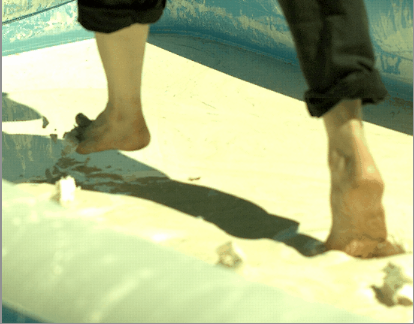
\includegraphics[width=6cm]{image/5-3-1.png}
\caption{在有``弹性''的液体上行走}\label{fig:oobleck}
\end{wrapfigure}
液体在很多方面与气体相似,\,而与固体区分来开.\,具体来说,\,液体没有固定的体积易于流动;\,没有弹性只有黏性;\,黏度与压缩系数比气体倒是大不少,\,这得益于其接近固体的高密度;\,热容,\,热导率等更细节的内容我们后几节详细阐述;\,微观细节则在以后章节中加以说明.\,最后,\,我们指出特殊条件下液体也具有某些与固体相似的性质,\,尤其是当变形率十分的急剧时.\,这种现象是\emph{非牛顿流体}(non-newtonian fluid)的一种典型,\,比如图\ref{fig:oobleck}中用玉米面粉与水和成的\emph{欧不裂}(oobleck)就是一种典型的一旦作用力变化十分快,\,就会主要表现出弹性固体的性质而不是液体的流动性的材料,\,所以人才可以在液面上快步走动而不会陷进去.\,但使我们把液体固体彻底区分开来的主要原因是因为固体具有\emph{序}(order),\,而且是\emph{长程}(long range)的序\footnote{凡事皆有例外,\,\emph{液晶}(liquid crystal)就有长程序的液体,\,\emph{非晶体}(non-crystalline)便是无长程序的固体.\,更准确的液体固体区分方式应该要看结合的强度.}.


液体内一般无序. 每一个单元周围的若干近邻粒子距离不像固体那样几乎取固定值, 也不像气体那样剧烈变化. 而是在一个特定的范围内分布. 用近邻粒子随半径的分布的方式来研究液体和固体气体的区别是一种行之有效的方法. 利用X射线衍射的方法可以得到物质内部单元之间距离分布的信息. 这样可以得到系统的\emph{径向分布函数}(radial distribution function), 即粒子体密度随与中心粒子距离的分布函数. 如图\ref{fig:rdf}所示为氩的三态的模拟计算后的径向分布函数.

\begin{wrapfigure}[12]{o}[-10pt]{8cm}
\vspace{-0.4cm}
\centering
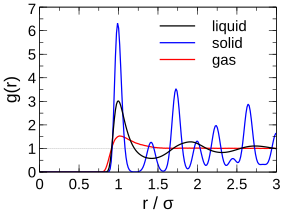
\includegraphics[width=8cm]{image/5-3-8.png}
\caption{径向分布函数}\label{fig:rdf}
\end{wrapfigure}
径向分布函数为``表'', 相互作用形式为``里''. 从径向分布函数可知:\, 气体仅有当两个分子较为靠近时径向分布函数才略有升高并随半径减小迅速趋于零, 从中可以分析出两个分子靠近则产生吸引, 势能降低, 玻尔兹曼分布下造成概率增加. 而通过固体径向分布函数可以看出即使在半径较大的情况下分子也具有长程序. 而液体则短距离下径向分布函数类似固体, 长距离下类似气体. 即在短距离下吸引力占据主导作用, 分子团可以形成局部的``类晶区'', 但是在长距离下则不具有平移不变性.

而如果考察液体分子之间相互作用的形式. 液体可以分为以下类型:

\begin{itemize}
\item \emph{范德瓦尔斯液体}(van der Waals liquid)

由无固有电偶极矩分子构成的液体, 其分子之间相互作用力为范德瓦尔斯力, 这是一种由于量子效应导致的与分子之间感应产生电偶极矩有关的力. 经验公式是为其引入前文也介绍过的\emph{李纳-琼斯势能}(Lennard-Jones potential):
\[V(r)=-\varepsilon  \left[ \left( \frac{\sigma}{r} \right)^6- \left( \frac{\sigma}{r} \right)^{12}\right]  \]

下一章相变将详细研究这种力同时造成的气体与液体的性质.

\item \emph{极性液体}(polar liquid):

构成液体的单元存在固有电偶极矩则为极性液体, 在极性液体中, 有存在一类单元之间有着较强吸引作用的液体, 水就是其中的典型代表. 称作\emph{缔合性液体}(associated liquid). 缔合性液体性质非常不同于非缔合性的对应液体, 热学上通常具有较大的黏滞, 反常的压缩与热容特性. 甚至会造成\emph{液液相变}(liquid-liquid phase transition, LLPT).

\item \emph{金属液体}(metallic liquid):

如果构成液体的基本可活动粒子带电, 如电子, 离子, 原子核. 那么这会大大增加液体内部的关联, 形成较好的导热和导电性能. 如熔解的金属, 稠密的等离子体等等.

\item \emph{量子液体}(quantum liquid):

在极低温或极高密等极端条件下的一些系统将会出现\emph{超流性}(superfluidity). 典型例子如$2.4{\rm K}$以下温度的液氦(${\rm {}^4He[II]}$). 它将体现出第二声(温度波), 热容发散, 黏度消失等奇特的力热效应.

\end{itemize}

即使对于我们最熟悉的液体水, 很多问题至今依然是开放问题与前沿问题: 如何准确描写水分子之间的相互作用? 冰和液态水之间的相变和液态水的反常膨胀是怎样的过程? 水一共有多少种物相? 诚然液体系统是复杂的多体问题, 其难点在于从自由的理想气体模型引入相互作用导致的高密度气体模型和从具有序的晶体模型不断引入序的破缺导致的瓦解的固体模型都不能很好地反应液体独特行为的全貌. 在理论研究液体行为的场合较多被使用的方法为\emph{密度泛函理论}(density functional theory, DFT). 对这个方法的介绍已经远远超出本书的范围. 故在以下对液体具体性质的讨论中我们将仅仅围绕现象进行介绍并做少量定性的原理注解.


\subsection{热容与黏度}
热容:\,一般来说,\,按原子的摩尔数计算,\,才有等压等体热容约为$3R$
热膨胀:\,部分液体与晶体反常膨胀,\,结晶过程也不是收缩反而是膨胀,\,一种解释是加热使得一些固体到液体成键倾斜以后更有利于在其他方向节省空间.

黏度:\,液体一般温度越高黏度越小.\,这是因为不同于气体黏度,\,液体黏度更像固体那样,\,靠的是相互作用形成的``激发''.\,而热运动加剧时液体分子间相互作用更难形成结果,\,比如两个原子很难形成一种亚稳态的``集团''.





\section{液体的表面性质}
\begin{itemize}
	\item 液体与气体交界面为\emph{表面}(surface),\,与固体交界面为\emph{界面}(interface).\,表面一般就若干个分子层那么厚,\,表面的分子数密度由于过渡到气体中所以明显会降低.\,界面则可能降低可能升高.
	\item 分子与分子间相互吸引形成内聚力,\,它的计算一般包括在体的内能中.\,但表面与界面的形成会改变能量,\,叫做表面能与界面能.\,它正比于其面积$S$.\,习惯上:
	\[W_s=+\sigma_s S=+\sigma_{\rm lg} S\]
	\[W_i=-\sigma_i S=-(\sigma_{\rm ls}-\sigma_{\rm gs})S\]

	前者$S$为液体表面面积.\,后者$S$为液体固体接触的界面面积,\,就是说要考虑由于液体与固体的接触使得固体与气体少接触了相同的面积可能导致的$\sigma_{\rm gs}S$能量,\,尽管这一项几乎总是可以忽略.\,$\sigma_{\rm ls}$是可正可负可为零的.\,$\sigma_{\rm lg}$一般大于零.

	\item 表面能对应\emph{表面张力}(surface tension):
	\[f_s=\sigma_s L\quad ;\quad f_i=\sigma_i L\]

	前者使表面尽可能小,\,后者使界面尽可能大.

	\item 附加压强的\emph{杨-拉普拉斯方程}(Young-Laplace equation):
	\[\Delta p=\sigma(\frac{1}{\rho_x}+\frac{1}{\rho_y})\]

	其中$\rho_x$和$\rho_y$是可以任意选取的两个相互垂直的方向上曲面上法曲线的曲率.

	\item 液体固体接触的\emph{接触角}(contact angle)的\emph{杨-杜普蕾方程}(Young-Dupr\'e)方程:
	\[\cos\theta=\frac{\sigma_i}{\sigma_s}\]

	若$\sigma_i>0$称为\emph{浸润}(wetting).\,若$\sigma_i>\sigma_s$上式无解称为\emph{完全浸润}(perfect wetting),\,液体会在固体表面尽可能铺展.\,若$\sigma_i\leq 0$称为\emph{不浸润}(non-wetting),\,若$\sigma_i<-\sigma_s$称为\emph{完全不浸润}(perfect non-wetting)

	\item 表面能实际上是自由能而不是内能,\,等温等压拉伸液膜要伴随着吸放热.\,详情参考之前章节的计算.

\end{itemize}



\section{极端条件下的其他物态}

\begin{itemize}
	\item 超冷($\sim {\rm \upmu K}$):\,\emph{玻色-爱因斯坦凝聚}(Bose-Einstein condensate):\,宏观数目的原子的动量$\bs{p}=\hbar \bs{k}$凝聚到了基态.\,其波函数可以被干涉实验探测到.
	\item 低温($1\sim 10{\rm K}$):\,\emph{超流}(superfluid)现象:\,如He-4液体黏度消失.\,He-3由于是费米子其超流直到1970年代才被发现,\,需要$\sim {\rm mK}$的低温.
	\item 低温物理中的高温($10\sim 100{\rm K}$):\,\emph{超导}(superconductor):\;常规金属的电阻率会消失,\,伴随着\emph{迈斯纳效应}(Meissner effect):\,完全抗磁性.\,电子结合成\emph{库珀对}(Cooper pair),\,可以像BEC那样通过晶格作用而凝聚成整个波函数而传播.

	\item 高温低密($10^3 \sim 10^4{\rm K}$):\,\emph{等离子体}(plasma),\,所有电子都与原子核不再形成束缚态,\,而是构成独立的气体体系,\,可以不考虑相对论效应也不考虑电子的量子简并来处理.\,

	\item 超高温,\,高密度($10^{11} \sim 10^{12}{\rm K},\,10^{17}{\rm kg/m^3}$):\,引力场下坍缩形成的中子星.\,电子数不再守恒而是在中子质子互变的反应中产生与消灭.\,

	\item 最高温($>10^{12}{\rm K}$):\,各大型对撞机上已经实现的\emph{夸克-胶子等离子体}(quark-gluon plasma):\,质子数和中子数不再守恒,\,内部的构成的夸克与胶子形成强相互作用的等离子体.\,

	\item 每一种粒子数不再守恒的极端相对论性的气体,\,其内能密度与温度的关系都是:\,对于每自由度的玻色子与费米子:
	\[u_b=\frac{2\sigma}{c}T^4\quad ;\quad u_f=\frac{7}{8}u_b\]

	例如对于光子气,\,两个偏振自由度再结合$J=uc/4$便得到黑体辐射公式.\,对于不包含第二代基本粒子的QGP,\,夸克有2味3色2自旋2电荷一共24自由度,\,胶子有8色2偏振(螺度)共16自由度.\,代入得:
	\[u=\frac{74\sigma T^4}{c}\]
\end{itemize}
%!TEX root = ../physical-olympics-2.tex
\chapter{相与相变摘要}


\section{相平衡}

\begin{itemize}
	\item 相平衡条件:\,等温等压,\,化学势相等:\,
	\[\mu_1(T,\,p)=\mu_2(T,\,p)\]

	即三种平衡同时被满足:\,热学,\,力学与化学平衡.

	\item 若$\mu_1>\mu_2$,\,粒子从势高的向势低的自发相变.\,如某温度下未饱和的水蒸气内化学势就会低于水中的化学势.

	\item 除了这三个量相等,\,摩尔熵$s$,\,摩尔体积$v$,\,数密度$n$两相平衡时都可以不相等.

	\item \emph{相变潜热}(latent heat)指等温等压条件下的吸热,\,所以是摩尔焓的增量:
	\[Q=\nu l=h_2-h_1=u_2-u_1+p(v_2-v_1)\]

	\item $0\cdgr$下若把水的比热容记做$1{\rm cal/g\cdot K}$,\,那么水的溶解热与汽化热为$80{\rm cal/g}$与$600{\rm cal/g}$,\,$100\cdgr$下汽化热降低到只有$540{\rm cal/g}$.\,冰和水蒸气的比热容几乎刚好只有水的一半$0.5{\rm cal/g\cdot K}$
\end{itemize}

\section{气液相变}
%\begin{wrapfigure}[9]{o}[-10pt]{7cm}
%\centering
%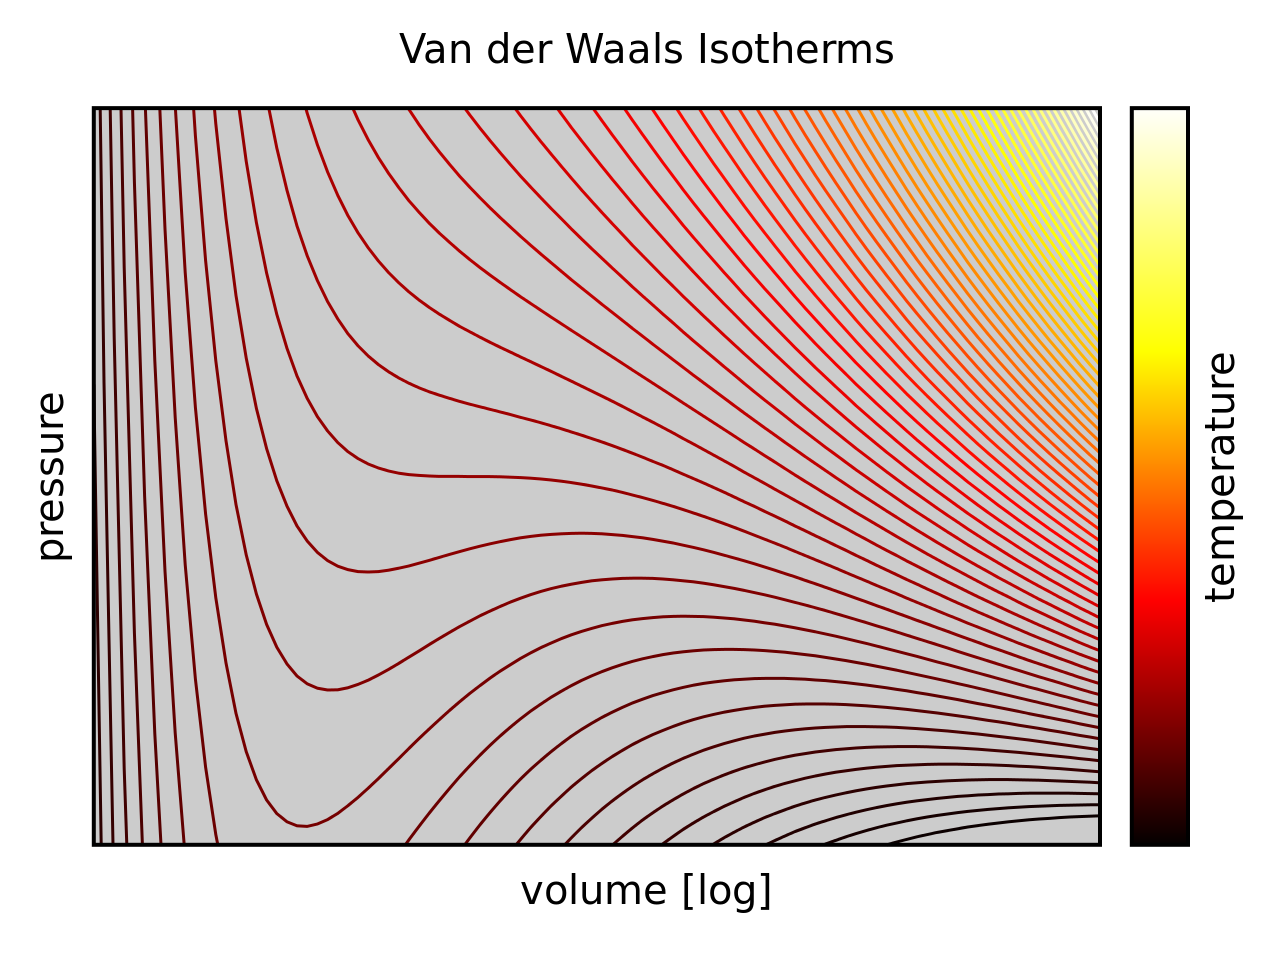
\includegraphics[width=7cm]{image/1.png}
%\caption{范氏等温线}
%\end{wrapfigure}
首先\emph{范德瓦尔斯方程}(van der Waals equation):
\[p=\frac{\nu RT}{V-\nu b}-\frac{\nu^2 a}{V^2}\]
\begin{itemize}
	\item 用范德瓦尔斯方程同时可以描述气体和液体,\,低于临界温度$T_c=8a/27Rb$时$p-V$曲线不再单调.\,提供了等温等压等化学势相平衡的可能性.\,事实上在\emph{麦克斯韦等面积法则}(Maxwell's equal area rule)决定的两点处能够相平衡.\,这定义了气液两相的分歧背后的数学原因.
	\item 汽化的熵变其实简单地决定了潜热:
	\[l=T(s_{\rm g}-s_{\rm l})\]
	\end{itemize}

	\begin{itemize}
	\item 两相共存时压强与温度的导数关系,\,也就是\emph{克劳修斯-克拉伯龙关系}(Clausius-Clapeyron relation):
	\[\frac{\ud p}{\ud T}=\frac{s_{\rm g}-s_{\rm l}}{v_{\rm g}-v_{\rm l}}=\frac{l}{T(v_{\rm g}-v_{\rm l})}\]
	
	\item \emph{蒸发}(evaporation):\,由于大气的存在,\,水蒸气在空气中仅是分压,\,不等于水的压强,\,但是大气压对水的压强使水压缩程度很小对水的化学势几乎可以忽略.\,故,\,可以认为某温度平衡时空气中的水汽分压就是该温度下水蒸气单独与水在该温度共存时的压强,\,称作\emph{饱和蒸气压}(saturate vapour pressure).\,$0\cdgr$时为$0.6{\rm kPa}$,\,室温下变成$2-4{\rm kPa}$,\,最后$100\cdgr$变成$1{\rm atm}$.\,蒸发条件是外界大气环境水蒸气分压不能达到该温度下的饱和蒸气压.\,这样化学不平衡会让水变成蒸汽而增大水面上的总压强,\,但是力学不平衡又会让蒸汽转移向上方的大气形成蒸发流.\,易挥发的气体会尤其明显.\,高压锅也是利用这个特点,\,取消了力学平衡,\,用化学平衡来使压强单方面增加.\,日常生活中的空气一般都是不饱和的,\,降雨的天气空气湿度可达$100\%$而形成饱和的空气.\,如果空气水蒸气分压较大而经历降温至\emph{露点}(dew point)以下,\,水蒸气就会析出而结露.

	\item \emph{沸腾}(boiling):\,当温度达到甚至高于某压强下两相共存对应的温度时.\,剧烈的沸腾现象就发生了.\,比如$1{\rm atm}$下水在$100\cdgr$沸腾,\,此时水蒸气不断产生希望在更高的压强下实现化学平衡,\,但是外界大气压的力学平衡又不允许.\,所以就发生了从内到外的剧烈汽化现象.
\end{itemize}

\section{连续相变}

\section{拓扑相变}
%!TEX root = ../physical-olympics-2.tex
\chapter{统计物理基础}

\section{数学基础}


\subsection{概率与独立性}
现实生活中有很多偶然事件,\,偶然事件的成因是多种多样的,\,它们集中表现在相似的条件下进行试验,\,而能够得到完全不同的结果.\,数学上用抽象的集合来表示所有可能的结果:
\[x\in X,\quad X=\{x\}\]

其中每一个元素代表一种可能的结果.\,这些结果应该有以下特点:
\begin{quote}
{\hei 忠实性}:\,每一个不同的实验结果如实地反应为集合中的不同元素.\,也就是不能用一个元素代替一类实验结果.\\
{\hei 互斥性}:\,当一个结果发生时,\,另一个结果就必须排除,\,也就是不能有多个元素对应同样的实验结果.\\
{\hei 完备性}:\,所有的实验结果必须都有集合中的元素对应.
\end{quote}

这样就能把集合\(X\)称为\emph{样本空间}(sample space),\,而每一个元素\(x\)也称为一个\emph{元事件}(elementary event).\,我们常说的\emph{事件}(event),\,其实一般指样本空间的一些定义良好的子集\(A\subset X\).\,只要实验结果在这个子集中,\,就说这个事件发生了.\,所谓定义良好我们可以做如下理解:

在\emph{古典概型}(classic models)情形下,\,样本空间是一个有限的集合,\,此时任意子集都可以视为某种事件.\,如投一颗骰子,\,样本空间为\(X=\{1,2,3,4,5,6\}\),\,则投出偶数是一个事件\(A=\{2,4,6\}\).

但在\emph{几何概型}(geometric models)情形下,\,样本空间一般具有与\(\mathbb{R}^n\)类似的结构,\,一般都是无限的集合,\,有一些``事件''的提法应当给予摒弃否则会引起矛盾.\,例如在闭区间\([0,1]\)间任取一个点,\,这个点恰好是有理数这样的``事件''可能就不是那么定义良好\footnote{事实上有理数集是定义良好---可测的,\,但有些集合不可测从而不能讨论它们的概率.\,参考\url{https://en.wikipedia.org/wiki/Non-measurable_set}}.\,一般常见的事件如点落在区间\((a,b)\)内等等.

设想同时做好几个实验,\,这几个实验互不干扰\,它们的结果是完全独立的,\,那么联合到一起就构成了一个大的实验,\,其结果应表示为一个数组:
\[\bs{x}=(x_i)\quad ;\quad x_i\in X_i\]

而新的样本空间称为原来那些样本空间的\emph{独立直积}(independent product).\,记做:
\[\bigotimes_i X_i=\{\bs{x}=(x_{ij})|x_{ij}\in X_i\}\]

互斥,\,独立这样的一些概念如何用数学严格表述?\,事实上它们恰恰是用概率去定义的.\,概率是一种我们关于实验结果可能性的\emph{先验假设}(a priori presumption),\,它是\emph{随机变量}(random variable)的正实数值函数\(P\),\,而随机变量既可以取为样本空间中的单个结果,\,也可以取为结果的集合:\,事件:
\[P(A)=P(\bigcup_{x_i\in A} {x_i})=\sum_{x_i\in A} P(x_i)\]

这其中已用到了\(P\)的属性:\,\emph{互斥事件}(mutual-exclusive events, disjoint events)的加法原理:
\[A\cap B=\emptyset\quad \Rightarrow\quad P(A\cup B)=P(A)+P(B)\]

再加上:
\[P(A)\geqslant 0\quad ;\quad P(X)=1\]

就构成了一个合适的概率定义.\,而对于随机变量可取连续样本空间,\,比如区间\([a,b]\)的情形,\,引入\emph{概率密度函数}(probability density function, pdf):
\[P([x,x+\ud x])=p(x)\ud x\quad ;\quad p(x)>0\;,\;\int_a^b p(x)\ud x=1\]

便是一个合适的概率定义.

现在来讨论事件的独立性.\,两个非互斥的事件可能同时发生,\,同时发生这一个新的事件即被定义为\(A\cap B\neq \emptyset\),\,此时可以定义事件\(B\)在事件\(A\)下的\emph{条件概率}(conditional probability):
\[P(B|A)=\frac{P(A\cap B)}{P(A)}\]

显然,\,若条件概率为零,\,那么实际上两个事件互斥.\,而实际上如果\(B\)在\(A\)下的条件概率等于\(B\)的概率,\,那么这种情况称为两个事件相互独立:
\[P(B|A)=P(B)\]

注意到上式实际上也可以写为:
\[P(X)P(A\cap B)=P(A)P(B)\]

所以两个事件相互独立的确是一个相互的关系,\,此时\(A\)的条件概率也有\(P(A|B)=P(A)\).\,两个事件相互独立是一种很微妙的关系,\,这意味着一个事件的发生既不会阻碍另一个事件,\,也不会促成另一个事件.\,而是完全没有影响.\,物理上看,\,很有可能两个事件没有因果关系.

我们之前构造的独立直积,\,用概率表示即为:
\[P((x_{ij}))=\prod_i P(x_{ij})\]

而对于连续概率分布,\,两个样本空间的独立直积给出的新概率应该是有以下概率密度:
\[p(x,y)=p_1(x)p_2(y)\]

\subsection{随机变量及其数字特征}
物理实验中的随机现象,\,常常体现为实验测量中测量结果数据的上下波动.\,此时一般认为这个测量数据\(x\)就是一个随机变量,\,而具有先验的某种概率密度函数\(p(x)\).\,.\,有时候我们关心测量数据的某种函数\(y=f(x)\),\,那么不同的\(y\)其出现概率分布应该修改:
\[p_y(y)=\frac{\ud p}{\ud y}=\frac{p(x)\ud x}{\ud y}=\frac{1}{f'}p(x)\]

例如,\,如果考虑在\(x\)方向的粒子速度\(v\)具有分布律:
\[p(v)=\frac{1}{\sqrt{2\pi}}\ue^{-\frac{v^2}{2}}\]

可以验证这个概率归一,\,那么其能量\(e=\dfrac{v^2}{2}\)的分布为
\[p_{e+}=\frac{p(v)}{v}=\frac{1}{2\sqrt{\pi e}}\ue^{-e}(v>0)\quad ;\quad p_{e-}=\frac{p(v)}{-v}=\frac{1}{2\sqrt{\pi e}}\ue^{-e}(v<0)\]

注意到同一个能量对应着两种可能的运动方向,\,故把两个\(\ud e\)对应概率分开算,\,最后合到一起:
\[p_e(e)=\frac{1}{\sqrt{\pi e}}\ue^{-e}\]

一个在统计中关心的数学处理,\,是在\(n\)次全同独立测量中获得的测量结果的\emph{平均数}(average):
\[\bar{x}=\frac{x_1+x_2+\cdots+x_n}{n}\]

而著名的\emph{大数定律}(law of large numbers)指出:\,如果概率分布的一个重要数字特征:\,\emph{期望}(expectation)存在\footnote{值得指出,\,有些数学上诡异的概率分布是不存在期望的,\,比如典型的柯西分布:
\[p(x)=\frac{\gamma/\pi}{x^2+\gamma^2}\]

当然这样的理想概率分布物理上几乎不存在,\,因为物理量总是有限的,\,在一定尺度下适用.}:
\[\mu=\langle x\rangle=\int x\ud p\]

那么如果随着测量次数趋于无穷,\,平均数将会无限趋近于期望值:
\[\lim_{n\to \infty}P(|\bar{x}-\langle x\rangle|>\varepsilon)=0\; , \; \forall \varepsilon>0\]

如何理解这一点?\,我们再定义另一个随机变量的数字特征:\,\emph{方差}(variance),\,物理上称为\emph{涨落}(fluctuation),\,数学上还称\emph{中心二极矩}(second central moment):
\[\sigma^2=\langle(x-\mu)^2\rangle=\int(x-\int x\ud p)^2\ud p\]

物理上还常常把涨落除以期望的平方称为相对涨落.\,那么可以证明:
\[\langle\bar{x}\rangle=\langle x\rangle\quad ;\quad \langle(\bar{x}-\mu)^2\rangle=\frac{\langle(x-\mu)^2\rangle}{n}\]

故随着实验次数增加,\,平均数作为新的随机变量它的期望不会变,\,而方差在不断减小,\,故有中心极限定理的说法.

以上讨论适用于任何\(y=f(x)\)型的随机变量,\,其中\(x\)可以是一次实验的实数结果,\,也可以是多次实验的数组结果,\,也可以是不同独立甚至非独立测量结果的复合,\,此时\(y\)即被理解为事件,\,代表某些可能发生的元事件的集合.\,期望与方差被定义为:
\[\mu=\int y\ud p\]
\[\sigma^2=\int (y-\mu)^2\ud p\]

其中\(\ud p\)表示\(y\)落在该点附近范围内的概率.

\subsection{信息熵}
为了刻画样本空间与其概率的多样性,\,我们引入\emph{信息熵}(information entropy)的概念.\,对于一个样本空间与随机分布,\,它具有的熵被定义为:
\[S=\sum_{x_i\in X}-P(x_i)\ln P(x_i)\]

而每一种可能性\(x_i\)带来的信息量被定义为\(I_i=-\ln P(x_i)>0\).\,而总熵是事件信息量的期望.\,为什么如此定义?\,比如我们设想投一枚骰子,\,那么投出\(1\)这个数的信息量应该是投出奇数的信息量加上在已知投出奇数后再投出\(1\)的信息量,\,投出奇数称作\(A\)事件那么这个性质写作:
\[I(x)=I(A)+I(x|A)\]

而应该有一种概率与信息量之间的普适对应,\,以上三个信息都可以理解为:
\[I(x)=f(P(x)),\,I(A)=f(P(A)),\,I(x|A)=f(P(x|A))\]

但三个概率本来就有:
\[P(x)=P(A)P(x|A)\]

这暗示着\(f(xy)=f(x)+f(y)\),\,在假定\(f\)性质足够好(可以求二阶导数)情况下:
\[\xrightarrow{\;\partial_y\;} xf'(xy)=f'(y)\]
\[\xrightarrow{\;\partial_x\;} f''(xy)+xyf'(xy)=0\]
\[\xrightarrow{xy=u\;} \frac{\ud}{\ud u}(u\frac{\ud f}{\ud u})=0\]
\[\Rightarrow f=C\ln u+C'\]

重新代入\(f\)性质,\,得\(C'=0\).\,剩下的\(C\)可以任取,\,一般理解为\(-1\),\,这样给出了正的信息量.\,这个推理过程还给出了事件的信息量\(I(A)\)与条件信息量\(I(A|B)\)两个概念的定义.\,根据定义,\,可见\(A\)取整个样本空间的信息量就是零.

现在我们理解到信息量表示稀有程度,\,具体事件发生概率越小则信息量越大.\,那熵又表示什么含义呢.\,它表示多样性.\,我们设想如果某一种元事件\(x_i\)的可能性被发现还可以细分为\(x_{i1},\,x_{i2},\cdots,x_{im}\)种子可能性.\,那么根据此式所引入的熵就会因此而增加,\,增量为:
\begin{align*}
\Delta S & = \sum_{j=1}^m -P(x_{ij})\ln P(x_{ij})-(-P(x_i)\ln P(x_i))\\
		 & = \sum_{j=1}^m -P(x_{ij})\ln P(x_{ij})-\sum_{j=1}^m -P(x_{ij})\ln P(x_i)\\
		 & = \sum_{j=1}^m -P(x_{ij})\ln\frac{P(x_{ij})}{P(x_i)}\\
		 & = \sum_{j=1}^m P(x_{ij})I(x_{ij}|x_i)\\
		 & = P(x_i)\cdot \sum_{j=1}^m -\frac{P(x_{ij})}{P(x_i)}\ln\frac{P(x_{ij})}{P(x_i)}\\
		 & = P(x_i)\cdot \sum_{j=1}^m -P(x_{ij}|x_i)\ln P(x_{ij}|x_i)\\
		 & = P(x_i) S(x_i)
\end{align*}

一方面,\,等于细化这一元事件所增加的信息量的概率平均.\,另一方面,\,也等于事件熵与概率的乘积.\,此处也定义了事件细分熵:
\[S(A)=\sum_{x_i\in A}-P(x_i|A)\ln P(x_i|A)\]

可见单个元事件的细分熵是零.\,而如果把样本空间可以分为一系列不相交的事件:
\[X=\bigcup_i A_i\quad ;\quad A_i\cap A_j=\emptyset(i\neq j)\]

那么有:
\[S(A)=\sum_i P(A_i)[I(A_i)+S(A_i)]=S(\{A_i\})+\sum_i P(A_i)S(A_i)\]

可见把不相交的事件并在一起时,\,总熵就是把\(A_i\)视作元事件的熵加上各个子事件的熵的加权和.

最后让我们来看看作为以上熵的定义所符合的一个十分重要的性质.\,为了方便起见我们把样本空间记做$\Omega$.\,并在样本空间的每个元事件引入两个随机变量$x_i\in X,\,y_j\in Y$.\,还要求两个随机变量独立:
\[P(x_i,y_j)=P(x_i)P(y_j),\,\forall i\forall j\]

那么对于整个样本空间按照随机变量$X$来划分的熵与$Y$的熵:
\[S_X=\sum_i -P(x_i)\ln P(x_i)\quad ;\quad S_Y=\sum_j -P(y_j)\ln P(y_j)\]

而总熵:
\[S=\sum_{ij}-P(x_i,y_j)\ln P(x_i,y_j)\]

计算其关系,\,容易发现:
\begin{align*}
S &=\sum_{ij}-P(x_i,y_j)\ln P(x_i)P(y_j)\\
  &=\sum_{ij}-P(x_i,y_j)\ln P(x_i)+\sum_{ij}-P(x_i,y_j)\ln P(y_j)\\
  &=\sum_{i}\sum_{j}-P(x_i,y_j)\ln P(x_i)+\sum_{j}\sum_{i}-P(x_i,y_j)\ln P(y_j)\\
  &=\sum_i -P(x_i)\ln P(x_i)+\sum_i -P(y_j)\ln P(y_j)\\
  &=S_X+S_Y
\end{align*}

即,\,独立随机变量的熵是可以直接相加的.\,而我们再来分析一下若是非独立随机变量的叠加导致的熵:
\begin{align*}
S_X+S_Y-S &=\sum_{ij}-P(x_i,y_j)\ln P(x_i)+\sum_{ij}-P(x_i,y_j)\ln P(y_j)-\sum_{ij}-P(x_i,y_j)\ln P(x_i,y_j)\\
	      &=\sum_{ij}-P(x_i,y_j)\ln\frac{P(x_i)P(y_j)}{P(x_i,y_j)}\\
	      &\geqslant -\ln\sum_{ij}P(x_i,y_j)\cdot\frac{P(x_i)P(y_j)}{P(x_i,y_j)}\\
	      &=-\ln\sum_{ij}P(x_i)P(y_j)\\
	      &=-\ln 1\\
	      &=0
\end{align*}


其中用到了$\ln$是上凸函数,\,所以自变量的加权平均处的函数值总是大于函数值的加权平均:
\[\ln(\sum_i p_ix_i)\geqslant \sum_ip_i\ln x_i\quad ; \quad \sum_ip_i=1\]

以上结论告诉我们非独立的两个随机变量所带来的熵有一部分是重合的,\,从而导致总的熵小于两个随机变量熵的和.\,小的这一部分叫做两个变量之间的\emph{互信息}(mutual information):
\[M=S_X+S_Y-S\]

互信息代表着已知一个随机变量的结果以后对另一个随机变量条件概率分布的影响.\,例如考虑自然光在某个方向的分振幅,\,以$x$方向的振幅作为第一个随机变量,\,如果另一个方向也是$x$,\,那么互信息恰好等于$x$方向振幅概率分布的熵;\,如果另一个方向为$y$方向,\,那么两个随机变量独立,\,从而互信息为$0$;\,如果选取一个与$x$方向夹锐角的方向,\,则$x$方向的振幅在一定程度上也会影响该方向的振幅的概率分布,\,从而两个随机变量之间具有一定的互信息量,\,并随着夹角增大到$90$度而消失.


\begin{itemize}
	\item 概率模型:\,\emph{经典概型}(classic models)中原子事件构成的集合是有限的,\,一般为等概率分布.\,也可以想象不是等概率的样本空间.\,事件是部分原子事件构成的子集.\,一般写作:
	\[x\in \Omega,\quad \Omega=\{\omega\}\]
	\[P(A)=P(\bigcup_{\omega_i\in A} {\omega_i})=\sum_{\omega_i\in A} P(\omega_i)\]
	\item 概率模型:\,\emph{几何概型}(geometric models)中的样本空间是与\(\mathbb{R}^n\)具有类似的结构的连续空间,\,一般认为参数化.\,比如原子事件抽象为区间$[a,\,b]$内的一个数,\,或是二维球面$S^2=\{(\theta,\varphi)|\theta\in(0,\,\pi),\,\varphi\in[0,\,2\pi)\}\cup\{\theta=0,\,\theta=\pi\}$上的一个点.\,而概率则是一个归一化的\emph{概率分布函数}(prabability distribution function):
	\[\int_a^b \ud p=\int_a^b p(x)\ud x=1\]
	\[\oint_{S^2} \ud p=\oint_{S^2} p(\theta,\, \varphi)\ud S=1\]

	\item \emph{独立事件}(indepedent events):\,对于经典概型,\,事件$A$与事件$B$独立:
	\[P(A\cap B)=P(A)P(B)\]

	如果把事件的交写作直接的乘积$A\cap B=AB$,\,事件的补$\Omega\backslash A$写作$\bar{A}$,\,上式等价于以下四式:
	\[P(AB)=P(A)P(B)\quad ;\quad P(A\bar{B})=P(A)P(\bar{B})\]
	\[P(\bar{A}B)=P(\bar{A})P(B)\quad ;\quad P(\bar{A}\bar{B})=P(\bar{A})P(\bar{B})\]

	在样本空间定义一个函数变量$X:\,\omega_i\mapsto x_i=X(\omega_i)$,\,那么可以根据不同的函数结果对样本空间进行分类,\,每一个结果就是一个事件,\,概率为$P(x_i)$.\,此时变量$X$与变量$Y$独立即定义为:
	\[\forall x_i\forall y_j:\,P(x_iy_j)=P(x_i)P(y_j)\]

	对于定义在$(x,\,y)\in \mathbb{R}^2$上的几何概型,\,概率分布关于两个坐标独立的条件为可以找到两个坐标各自的概率分布函数:
	\[\forall x\forall y :\,p(x,\,y)=p_x(x)p_y(y)\]

	\item 两种概型下变量$X$的\emph{期望}(expectation)$E=\langle X\rangle $与\emph{方差}(variance)$\sigma^2=\langle (X-E)^2\rangle$的定义:
	\[E=\sum_{\omega_i\in \Omega} P(\omega_i)X(\omega_i)=\int_\Omega X(x)\ud p\]
	\[\sigma^2 =\sum_{\omega_i\in \Omega} P(\omega_i)(X(\omega_i)-E)^2=\int_\Omega (X(x)-E)^2\ud p\]

	\item 两种概型下\emph{统计熵}(statistic entrophy)或\emph{信息熵}(information entropy)的定义:
	\[S=-\sum_{\omega_i\in \Omega} P(\omega_i)\ln P(\omega_i)=-\int_\Omega \ln P(x)\ud p\]

	\item 在$\mathbb{R}$上的分布若要求$\sigma^2$取固定值,\,那么\emph{正态分布}(normal distribution)可以使得熵最大:
	\[p(x)=N(\mu,\,\sigma^2)=\frac{1}{\sqrt{2\pi }\sigma }\ue^{-\frac{-(x-\mu)^2}{2\sigma^2}}\]

	如果还要求期望为零,\,那么上式$\mu=0$.\,注意这等价于说,\,如果一个一维粒子的平均动量为$0$而平均动能为$\langle mv^2/2\rangle=kT/2$,\,熵最大的分布为:
	\[f(v)=\sqrt{\frac{m}{2\pi kT}}\ue^{-\frac{mv^2}{2kT}}\quad ;\quad S=\ln\sqrt{\frac{m}{2\pi kT}}-\frac{1}{2}\]

	\item 如果已知$\mathbb{R}^2$上概率分布$p(x,\,y)$的\emph{边缘分布}(marginal distribution)$p_x,\,p_y$:
	\[p_x(x)=\int_{-\infty}^\infty p(x,\,y)\ud y\]
	\[p_y(y)=\int_{-\infty}^\infty p(x,\,y)\ud x\]

	那么在$\mathbb{R}$分别以$p_x,\,p_y$作为分布函数的分布的熵与二维分布的熵满足:
	\[S\leq S_x+S_y\]

	成立条件是$X$与$Y$随机变量独立:
	\[p(x,\,y)=p_x(x)p_y(y)\]

	这就是说,\,两个随机分布合成时,\,独立合成能够使得熵最大.

\end{itemize}

\section{统计假设}

原则上来说,\,经典的物理体系应当是\emph{确定性}(certainty)的,\,用经典力学语言可以描述(质点系的位置与动量)的,\,不包含\emph{随机性}(randomness)的,\,不应引入概率描述的系统.\,然而一方面由于体系在大粒子数大自由度数下所体现出来的统计复杂性,\,即使初态是一个高度特殊的状态:\,比如一个长方体气缸内理想气体初始时刻所有粒子排列为规则的点阵,\,具有完全相同的速度矢量.\,在历经一段时间之后也会体现出完全的随机性:\,体系在很长一段时间内看来各个状态都没有明显的\emph{序}(order),\,显得杂乱无章.\,而稍微有序的状态几乎不可能再次出现.\,这期间的过程与演化,\,原则上说理应是确定性的过程,\,如果我们在某一时刻命所有粒子的速度方向反向,\,这个体系将会重新回到最初的状态.

但是我们将研究\emph{随机过程}(stochastic process),\,在一个随机过程中,\,即使上一刻只有唯一的一种状态,\,下一刻的状态也不是决定性的,\,而是体现出不确定性或是随机性.\,从而对一个时刻系统完整的描述就要包含在各种可能状态下的概率,\,这实际上是一个\emph{系综}(ensemble).\,用系综而不是单个的系统描述,\,从而引入概率的原因有以下几个:

\begin{itemize}
	\item 外在随机性:\,多自由系统是混沌系统,\,初态微小的改变将会随时间以指数形式迅速放大.\,热力学体系总是处在外界环境中,\,外界总是对体系有各种各样的微小扰动.\,即使在之前的情况下在某个时间让所有粒子速度反向,\,也会因为外界对体系的影响而无法观察到体系回到初始状态.
	\item 内在随机性:\,以衰变为例,\,如果认为衰变发生在一个瞬间,\,粒子只可能处于衰变前或衰变后两个不同状态,\,那么衰变就是一个随机的过程.\,每一小段时间粒子均以均等的概率衰变,\,那么大量全同未衰变的粒子构成的体系的未衰变数期望随时间将指数衰减,\,但是每一个时刻未衰变粒子数仍然具有某种概率分布,\,粒子数对于其期望仍具有某种方差.\,事实上原子与原子的碰撞涉及到量子力学行为,\,同样的初始条件是会导致不同的结果的.
\end{itemize}


\begin{itemize}
	\item \emph{等概率原理}(principle of equal a-priori probability):\,平衡态分布在相空间等能量曲面上所有点处的概率分布函数都应该相等.\,例如大量摆角固定的单摆构成的热力学体系,\,显然摆球出现在最高点的概率要大于最低点的概率(最高点速度慢停的久).\,但是如果把其摆动的$p-x$空间画出来合适的比例下相轨迹为圆,\,而且一定做匀速圆周运动,\,所以肯定单位圆弧上出现摆球的概率相等.\,这个结论是理论力学里通过\emph{刘维尔定理}(Liouville's theorem)的一种合情推理,\,但一般作为平衡态统计力学的最初假设.

	\item 通过等概率原理可以证明,\,如果理想气体也符合这个原理的话,\,平衡态分子速度作为随机变量分布为麦克斯韦分布律.\,这个推导参考热力学统计物理书籍的系综理论.
	\item 通过等概率原理+求\emph{最可几分布}(most probable distribution)也可以得到实际的分布为麦克斯韦分布律.\,这个推导也参考热力学统计物理书籍的最可几分布.
	\item \emph{玻尔兹曼H定理}(Boltzmann H theorem):\,通过\emph{分子混沌假说}(molecular chaos hypothesis),\,认为从非平衡态分子通过碰撞向平衡态转变的过程中,\,每一时刻都存在的概率分布,\,即,\,真实世界的情况只是万千可能情况中的一种.\,而每一次分子的碰撞都是把单一的初态的可能性变成了更多的末态的可能性.\,数学上很容易证明,\,这样的概率演化过程熵只增不减.\,从而末态的熵一定达到了极值.\,再根据上一章的论述,\,粒子在三个方向的速度分布一定是正态分布,\,且彼此独立,\,平均动能一致时熵最大.\,也给出了麦克斯韦分布律.
\end{itemize}


\section{麦克斯韦分布律}

三维\emph{麦克斯韦速度分布律}(Maxwell distribution law)是指:
\[f(\bs{v})=\left(\frac{m}{2\pi kT}\right)^\frac{3}{2}\ue^{-\frac{m\bs{v}^2}{2kT}}=\prod_1^3 \sqrt{\frac{m}{2\pi kT}}\ue^{-\frac{mv_i^2}{2kT}}\]

\begin{itemize}
\item 这是速度空间中的概率分布函数. 即若分子数$N$很大则$\ud N = Nf(\bs{v})\ud v_x\ud v_y\ud v_z$.

\item 由于三个方向分布律独立, 每个方向上的分布律也叫麦克斯韦速度分布律:
\[ \sqrt{\frac{m}{2\pi kT}}\ue^{-\frac{mv_i^2}{2kT}}\]
\[f(\bs{v})=f(v_x)f(v_y)f(v_z)\]

\item 麦克斯韦速率分布律是指速度空间中等速率球之间的概率微元决定的函数:
\[\frac{\ud N}{N}=\ud p=F(v)\ud v \]
\[F(v)=4\pi v^2\left(\frac{m}{2\pi kT}\right)^{\frac{3}{2}}\ue^{-\frac{mv^2}{2kT}}\]

\item 平均速率与方均根速率:
\[\overline{v}=\sqrt{\frac{8kT}{\pi m}}\quad ;\quad \sqrt{\overline{v^2}}=\sqrt{\frac{3kT}{m}}\]

\item 泻流数与压强既可以用速率分布计算也可以用单方向的分布函数计算:
\[\varGamma=\frac{1}{4}n\overline{v}\quad ;\quad \ud \varGamma=\frac{1}{4}\ud nv\]
\[p=\frac{2}{3}n\overline{\varepsilon}\quad ;\quad \ud p=\frac{2}{3}\ud n\varepsilon\]

\item 光子气的以上公式是类似的:
\[\varGamma=\frac{1}{4}nc\quad ;\quad \ud \varGamma=\frac{1}{4}\ud nc\]
\[p=\frac{1}{3}n\overline{\varepsilon}\quad ;\quad \ud p=\frac{1}{3}\ud n\varepsilon\]
\end{itemize}

\section{能均分定理}

\begin{itemize}
	\item \emph{近独立子系}(nearly independent system): 体系的内能可以写出各个粒子内能的和, 即忽略粒子之间的相互作用或者做\emph{平均场}(mean field theory)处理:
	\[U=\sum u_i=\sum h(q_i,\,p_i)\]

	\item \emph{玻尔兹曼分布律}(Boltzmann distribution law): 若粒子在某一自由度上的能量为$h(q,\,p)$, 那么概率即为:
	\[\ud p=C\ue^{-\frac{h(q,\,p)}{kT}}\ud p\ud q\]

	其中$p$为该自由度上的广义动量, $C$为归一化常数, 可积分计算. 或者直接我们写出最关心的平均能量:
	\[u=\frac{\iint h(q,\,p)\ue^{-\frac{h(q,\,p)}{kT}}\ud p\ud q}{\iint \ue^{-\frac{h(q,\,p)}{kT}}\ud p\ud q}\]

	\item 每一个平方项形式的能量在麦克斯韦分布律下都具有如下相同的平均能量:
	\[\overline{\frac{1}{2}M\dot{q}^2}=\overline{\frac{1}{2}Kq^2}=\frac{1}{2}kT\]
	\item 非平方项故不符合能均分的例子: 重力场, 离散线性能级, 二能级系统, 三维电偶极子...
\end{itemize}

\section{功, 热, 熵}

\begin{itemize}
	\item 通过以上近独立子系的分析可以发现, 体系的内能为温度和哈密顿量中参数(比如系统的体积等整体广义坐标)的函数:
	\[U=Nu=U(T,\,Q_\alpha)\]
	\[u=\iint h(q,\,p,\,Q_\alpha)\rho (q,\,p,\,Q_\alpha,\,T)\ud p\ud q\]
	\[\rho (q,\,p,\,Q_\alpha,\,T)=\left.\ue^{-\frac{h(q,\,p,\,Q_\alpha)}{kT}}\middle/\iint \ue^{-\frac{h(q,\,p,\,Q_\alpha)}{kT}}\ud p\ud q\right.\]
	\item 绝热功: 在一个过程中, 哈密顿量中参数改变, 温度改变, 导致分布不变:
	\[\ud\left(\frac{h(q,\,p,\,Q_\alpha)}{kT}\right)=0\quad \Rightarrow \quad\ud \rho (q,\,p,\,Q_\alpha,\,T)=0\]
	\[\ud u|_{\rm diabatic}=\iint \ud h(q,\,p,\,Q_\alpha)\rho (q,\,p,\,Q_\alpha,\,T)\ud p\ud q\]
	\[\ud U|_{\rm diabatic}=\sum Y_\alpha \ud Q_\alpha\]

	\item 热: 内能改变的其他部分:
	\[\ud q=\ud u-\ud u|_{\ud Q=0}=\iint h(q,\,p,\,Q_\alpha)\ud \rho (q,\,p,\,Q_\alpha,\,T)\ud p\ud q\]

	\item 熵: 容易证明, 如果定义:
	\[s=\frac{u}{T}+k\ln \iint\ue^{-\frac{h(q,\,p,\,Q_\alpha)}{kT}}\ud p\ud q\]

	则有:
	\[\ud q=T\ud s\]
\end{itemize}


%\section{量子与相对论}

%\begin{itemize}
	%\item 

	%\item 

	%\item 
%\end{itemize}


%!TEX root = ../physical-olympics-2.tex
\chapter{光波与光线}

\section{界面上的反射与折射}

\subsection{光波与光线}

众所周知,\,光是电磁频谱的一段.\,我们所说的光一般是指\emph{可见光}(visible light),\,学术上代表波长为$400-700{\rm nm}$的电磁辐射.\,它大致代表了人对光的色视觉的界限.\,而一般的光学研究还包括了波长长至$1{\rm mm}$左右的\emph{红外光}(infrared light,\,IR)与短至$10{\rm nm}$的\emph{紫外光}(ultraviolet light,\,UV).
\begin{figure}[H]
\centering
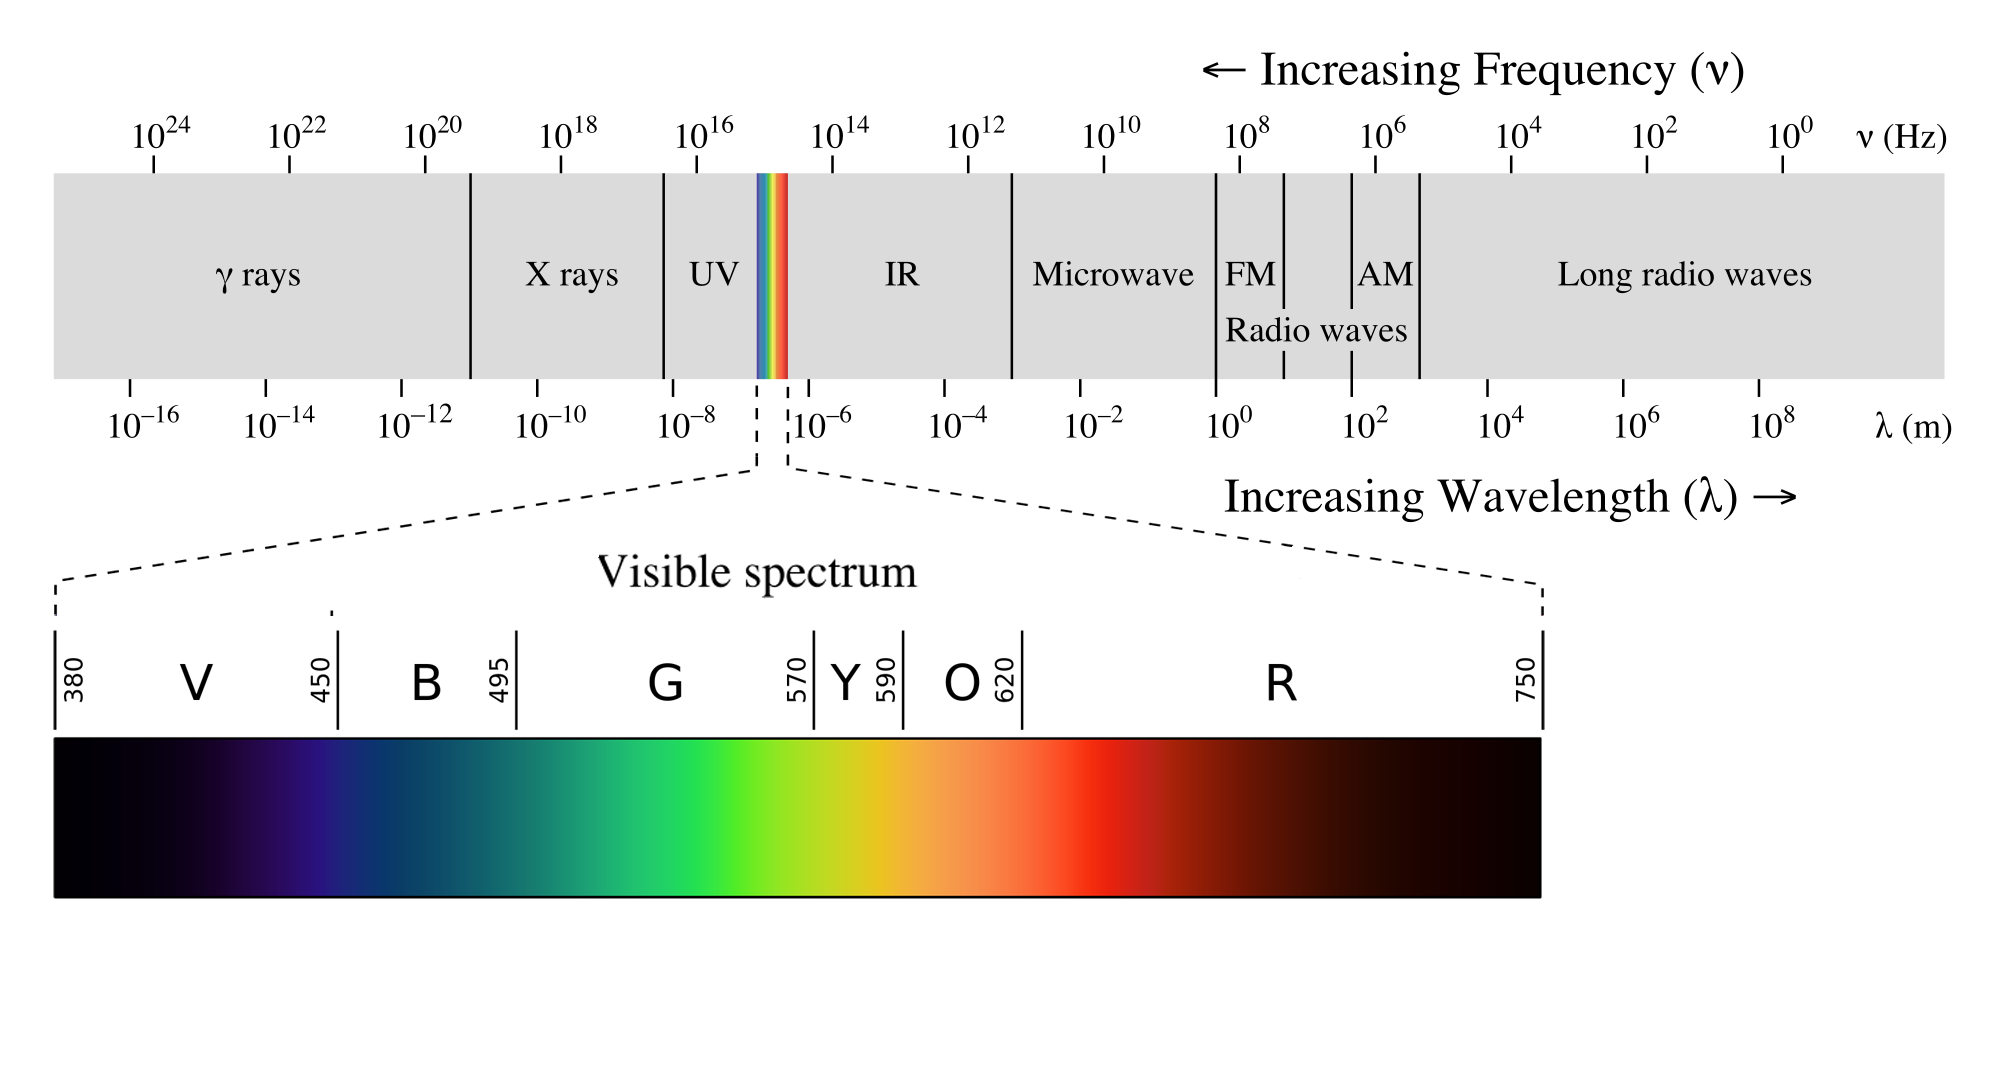
\includegraphics[width=0.8\textwidth]{image/5-6-1.png}
\caption{光学研究范围}
\end{figure}

\begin{wrapfigure}[14]{o}[-10pt]{7cm}
\centering
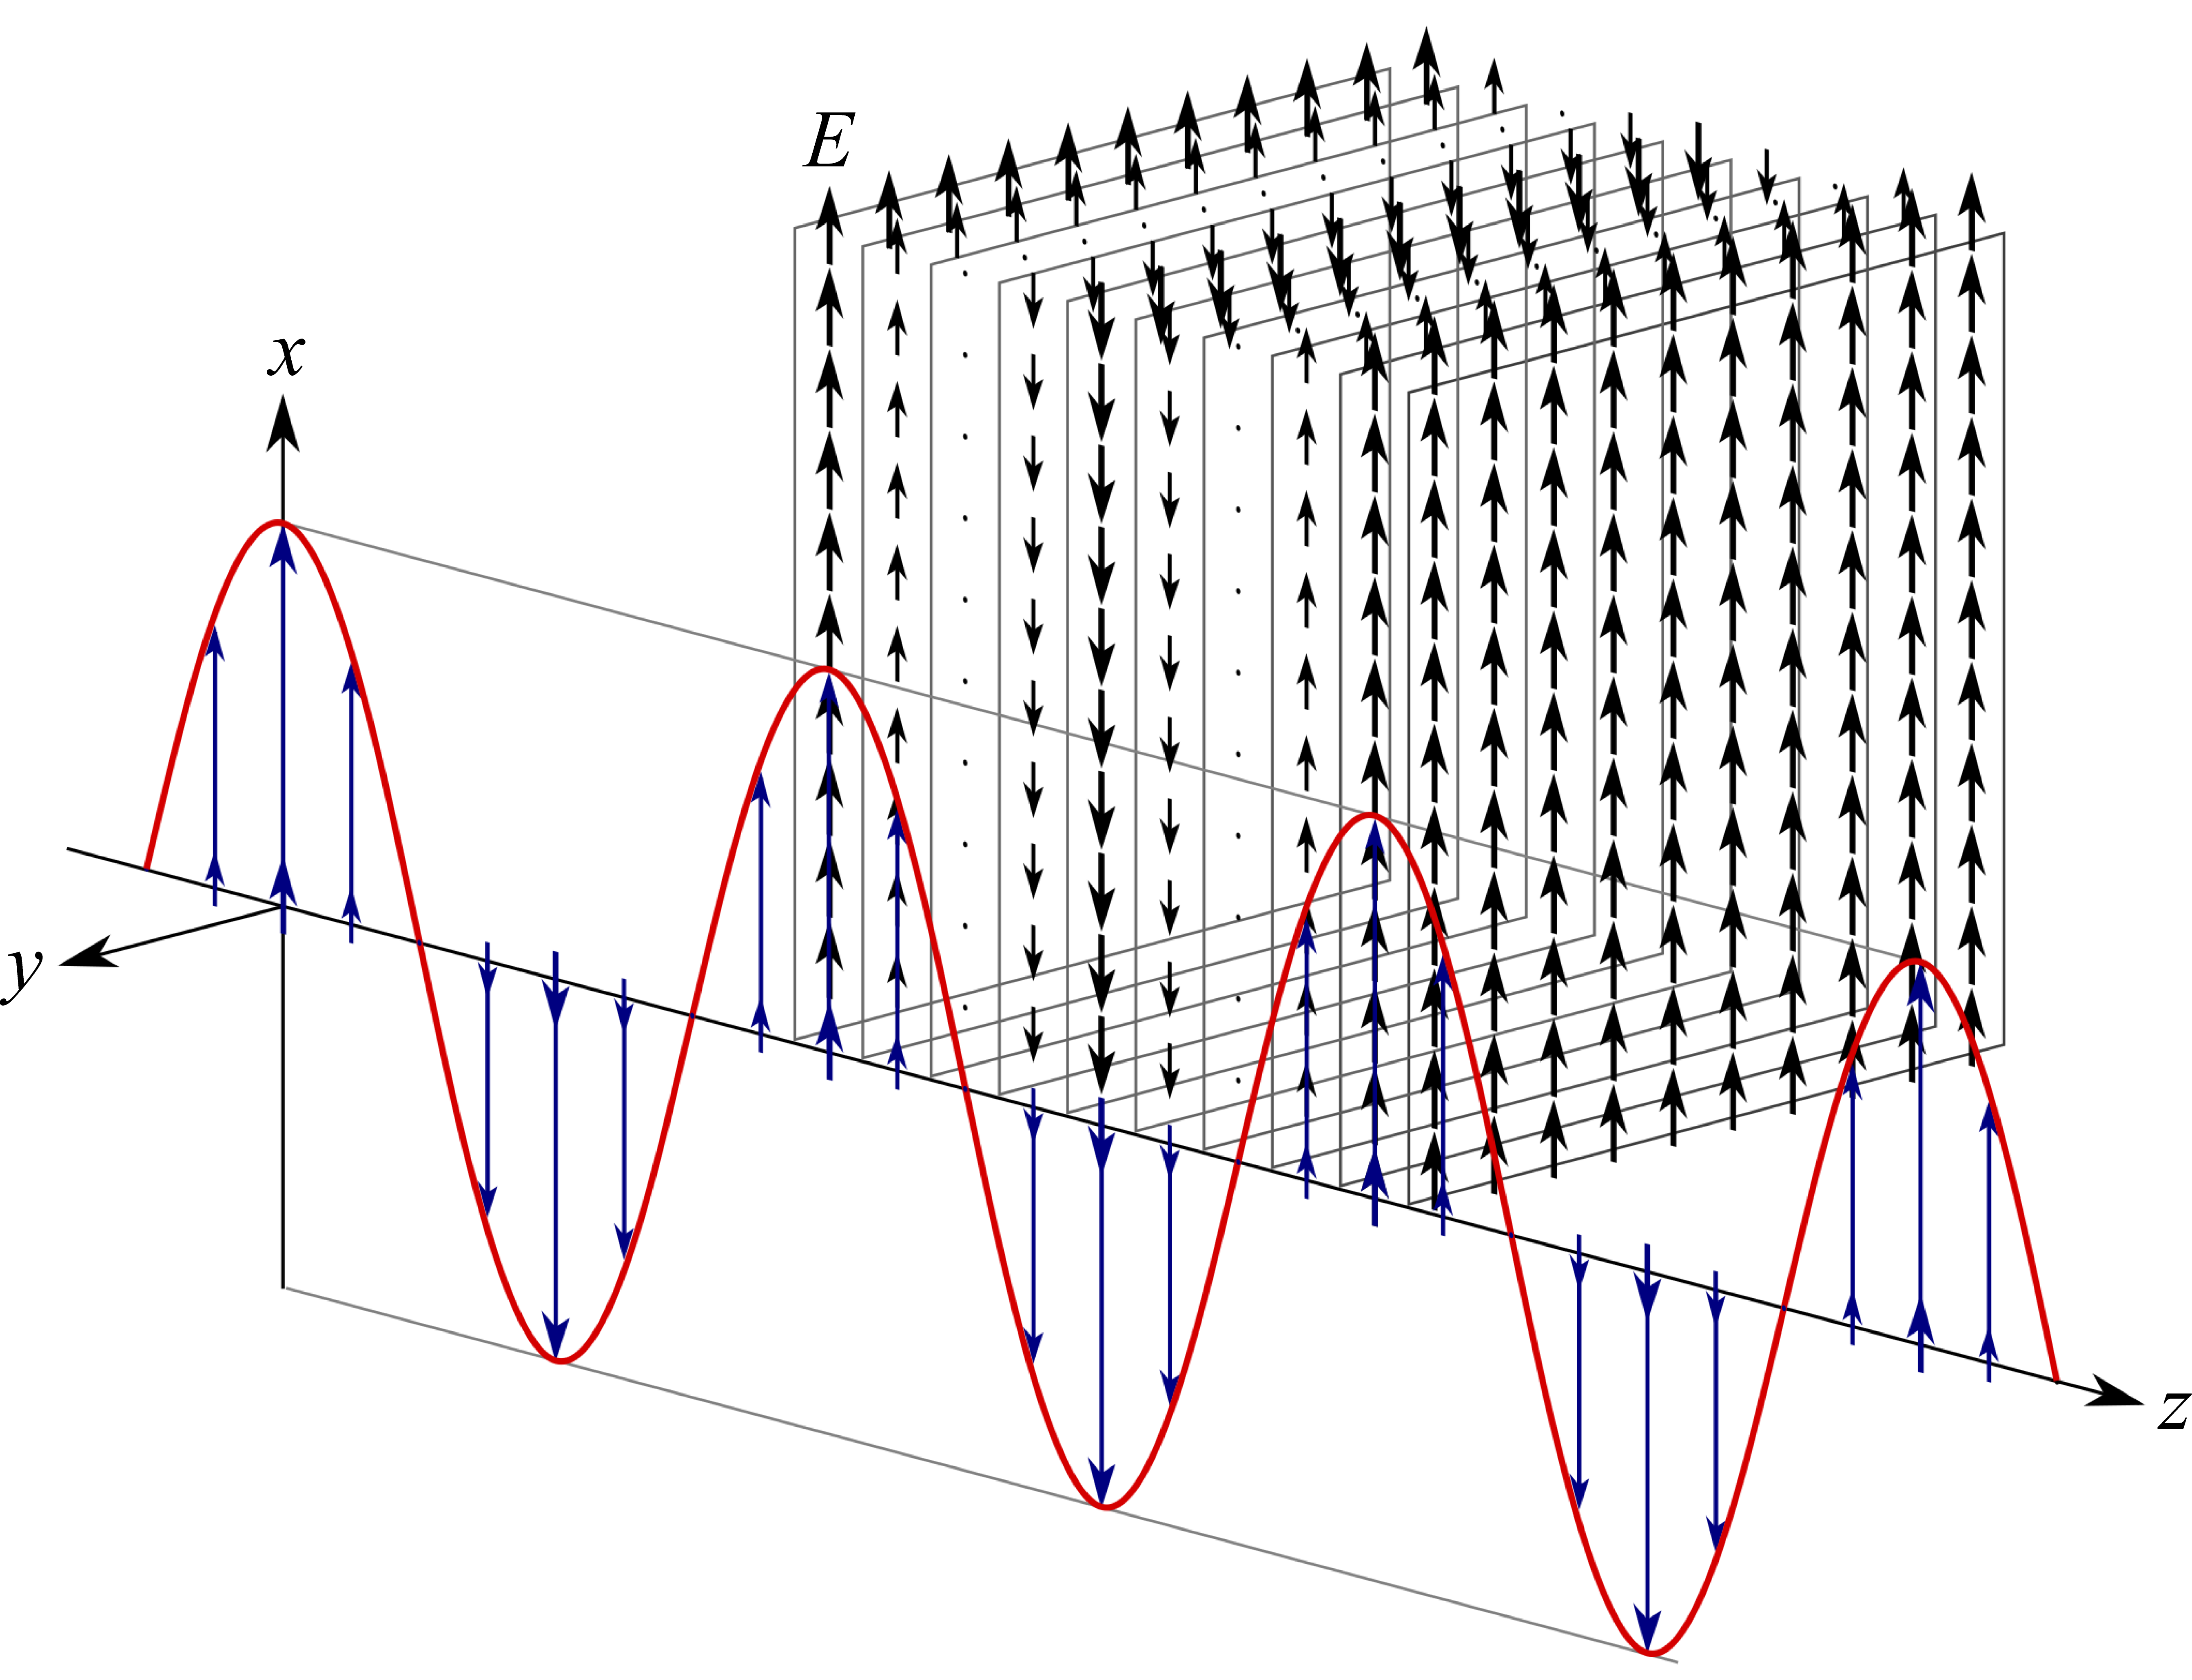
\includegraphics[width=8cm]{image/5-6-2.png}
\caption{平面偏振电磁波}
\end{wrapfigure}
光的波动理论建立在众多干涉衍射实验上,\,由19世纪后半页麦克斯韦({\it Maxwell}),\,韦伯({\it Weber})与赫兹({\it Hertz})等人的理论与实验工作进行总结与升华.\,最后通过迈克尔孙({\it Michelson})的干涉实验和随之由爱因斯坦({\it Einstein}),\,洛伦兹({\it Lorentz})等人建立的狭义相对论来完善与归入到更加普适的经典电磁场论下.\,然而整个18世纪实际上都处于光的粒子学说与波动学说的无休止争论中.\,这是因为此时发现的光的几乎所有现象都可以同时用两种学说进行解释.\,今天我们知道了光实际上也有\emph{波粒二象性}(particle-wave duality),\,最准确的描述光的语言应该是\emph{量子电动力学}(quantum electrodynamics,\,QED).\,光是一份份的量子场,\,被称为\emph{光子}(photon).\,几何光学问题,\,用经典的电磁场模型给出的描述最为精确,\,而在特殊场合或者精度要求不高的情况下,\,粒子光学的处理也是十分合适的.

真空中的\emph{平面波}(plane wave)提供了一种最为简单的情形,\,如图,\,此时$\bs{E}=E\bs{e}_x\cos(\omega t-kz)$.\,按照光学惯例,\,我们把它写作一个复数,\,模就是在每一点处场强的振幅,\,而幅角我们取为$\cos$里的相位宗量的相反数,\,而它的实部表示物理上的场强:
\[A(z,t)=E\ue^{\ui(kz-\omega t)}\]

有几点值得注意:\,首先,\,之所以取相反数,\,是因为在频率甚高的光频波段我们不太用关心每一个时空点处场随时间$t$的变化,\,而是不同时空点$z$对振幅与相位的影响,\,故把$kz$项提前.\,而对于$\omega t$项由于每一点的振动都含这个随时间振动的因子,\,而且角频率都是$\omega$(单色波),\,所以我们往往又省去这个因子写成$A=E\ue^{\ui kz}$,\,相当于仅考虑$t=0$时的初相位与振幅.\,这种操作意味着指数上的宗量随时间减小,\,这与我们平时对相位随时间增加的理解是相反的.\,其次,\,我们取消了其矢量性,\,我们知道沿特定方向$z$传播的平面单色电磁波可以分解为$x$方向的偏振与$y$方向的偏振,\,两者的同相反相组合可以造成不同方向的\emph{线偏振模式}(linear polarized mode),\,而相差$\dfrac{\pi}{2}$的组合则可以造成不同的\emph{圆偏振模式}(circular polarized mode).\,但这些只有在特殊的光学器件下进行偏振光干涉实验才能发现区别,\,故在一般的几何光学条件下我们只关心光的传播方向,\,相位与振幅信息,\,而不关心其偏振时用标量$A$来代表任意模式下约化的光的振幅大小,\,$A$具有电场强度的量纲\footnote{这是因为与物质发生相互作用而感光时电场的作用占据主导地位.},\,相同的$A$代表相同的光强与能流.\,$A$被称为\emph{标量振幅}(scalar amplitude).

平面波是其他一大类波在局部可以采取的近似,\,我们把等相位的面在局部近似为平面,\,则波传播方向为垂直于平面的法线方向,\,用\emph{波矢}(wave vector)$\bs{k}$代表这个方向,\,它的大小就是上述平面波的$k$,\,代表单位长度所改变的相位大小,\,正如\emph{角频率}(angular frequency)代表单位时间所改变的相位大小.\,两者具有如下关系:
\[\frac{\omega}{k}=\frac{\nu}{\sigma}=\frac{\lambda}{T}=\frac{c}{n}\]

其中$\nu$表示\emph{频率}(frequency),\,单位时间所经历的振动周期数,\,由于一个周期相位改变$2\pi$,\,故$\omega=2\pi \nu=\dfrac{2\pi}{T}$,\,同理,\,$\sigma$表示\emph{波数}(wave number),\,有$k=2\pi \sigma=\dfrac{2\pi}{\lambda}$,\,$\lambda$表示\emph{波长}(wave length)而$T$表示\emph{周期}(period).\,这里考虑到介质中的传播,\,波速小于真空中的波速,\,$n$为介质的\emph{折射率}(index of refraction).

而我们所要研究的更加普遍的一类光波一般写为:
\[A(\bs{r})=E(\bs{r})\ue^{\ui \varphi(\bs{r})}\]

这类光波的共性是仍然以统一地角频率$\omega$振动,\,也就是所谓的\emph{单色波}(monochromatic wave)\footnote{此时波的波动方程变为亥姆霍兹方程:\[\left[\nabla^2-\frac{1}{(c/n)^2}\frac{\partial^2}{\partial t^2}\right]A\ue^{-\ui \omega t}=0 \quad \Rightarrow \quad (\nabla^2+k^2)A=0\]}.\,所以我们省去包含时间的因子$\ue^{-\ui \omega t}$,\,直接写出只依赖于位矢$\bs{r}$的波动形式.\,一般来说$E$是$\bs{r}$的缓变函数,\,而$\varphi$则是$\bs{r}$的快速变化函数,\,且其变化要与波矢大小$k=\omega/c$相吻合:
\[\nabla \varphi=\bs{k}\]

例如,\,波源在$\bs{r}=0$的\emph{球面波}(spherical wave)有$E=\dfrac{u}{r},\,\varphi=kr$,\,而波源在$\rho=0$的\emph{柱面波}(cylindrical wave)有$\displaystyle E=\frac{u}{\sqrt{\rho}},\,\varphi=k\rho$.

\begin{figure}[H]
\centering
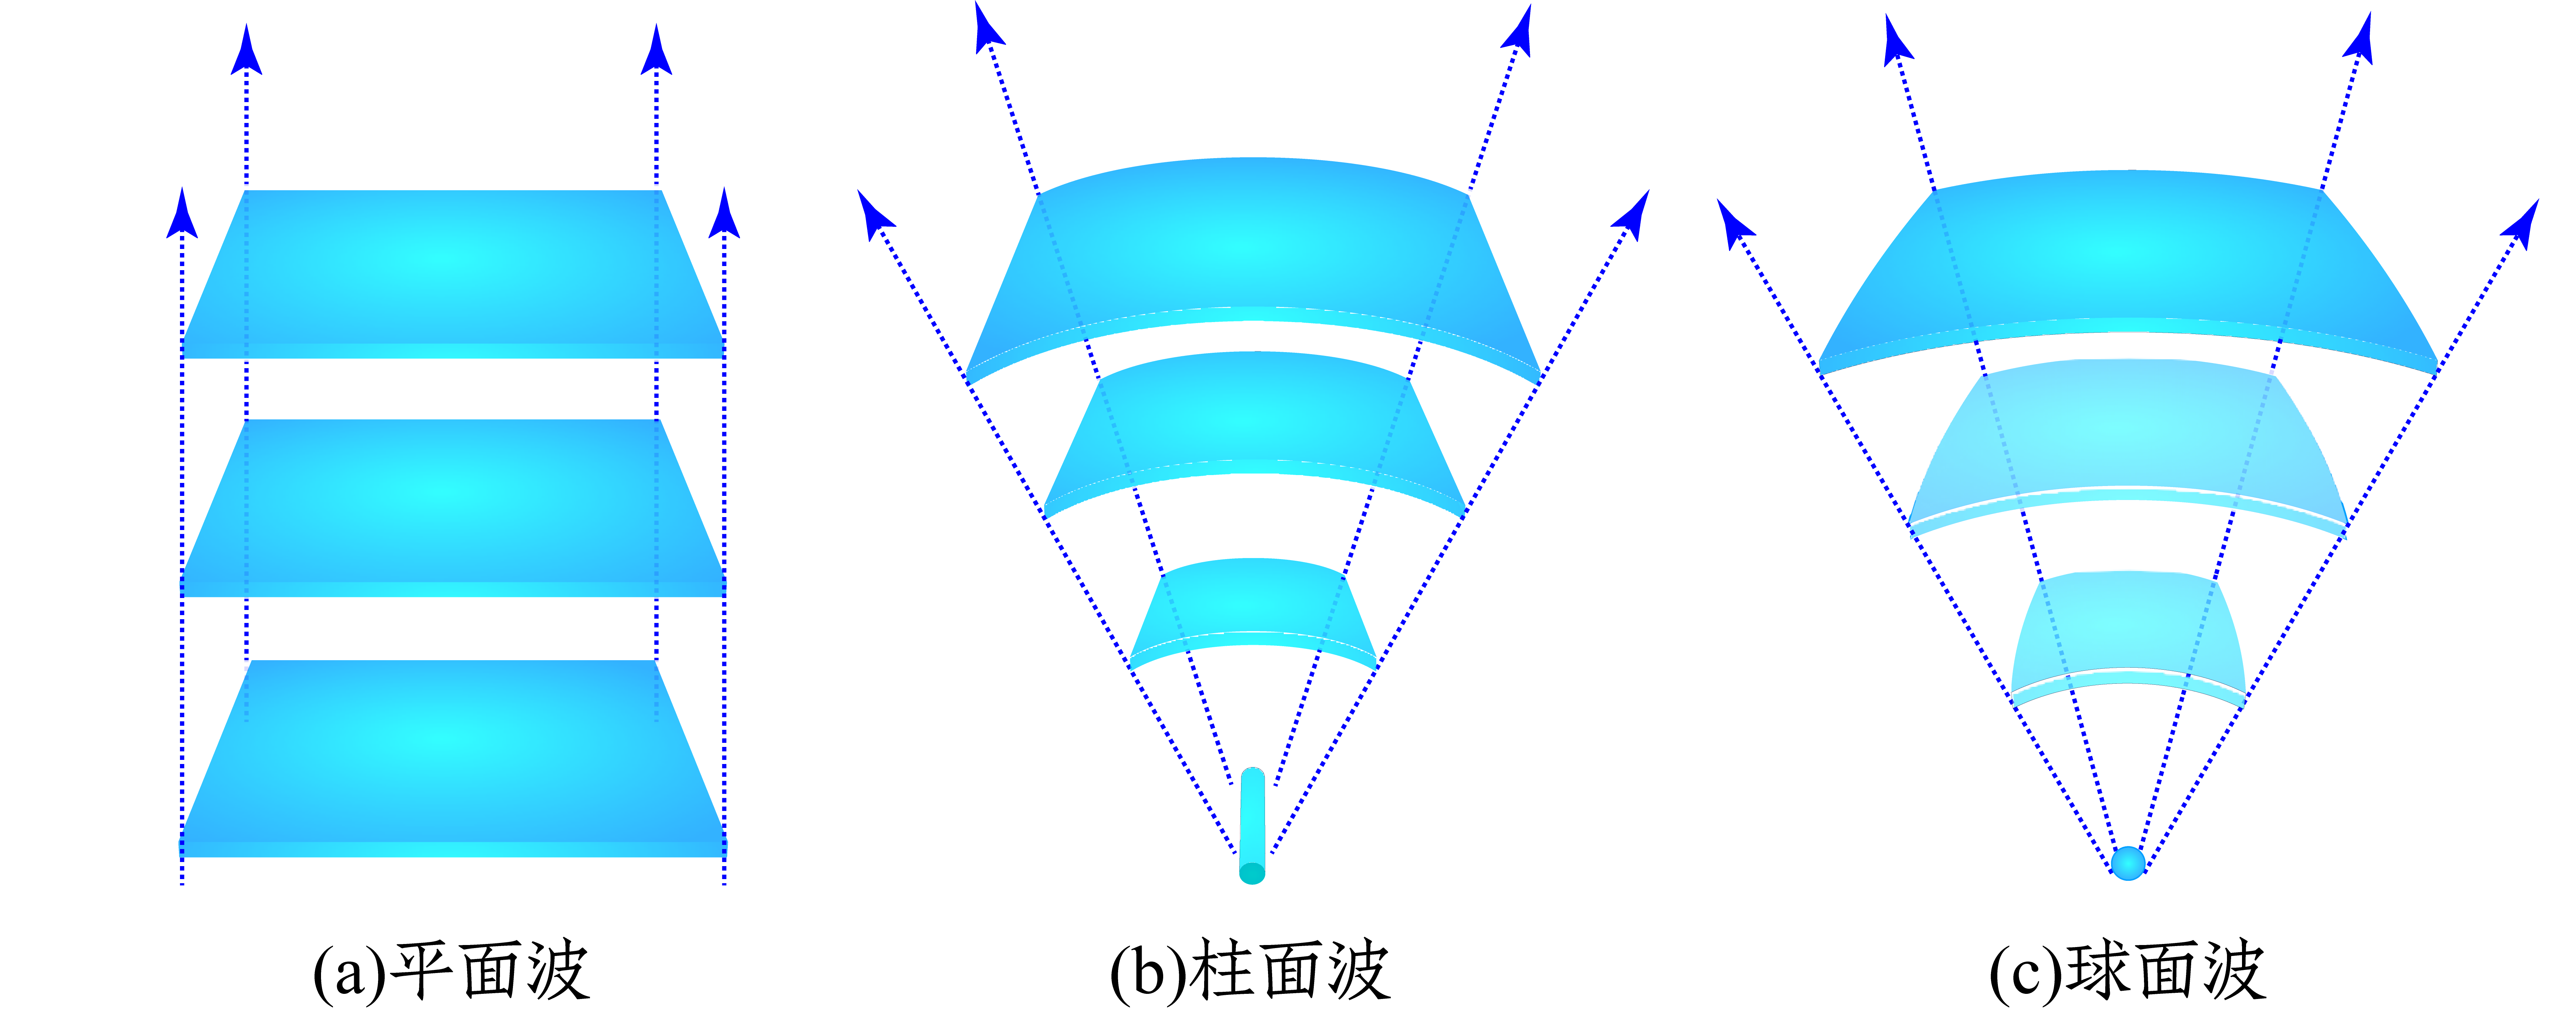
\includegraphics[width=0.8\textwidth]{image/5-6-3.png}
\caption{三种常用波形式}
\end{figure}

显然这些理想的波不能看成是生活中的一般光源的波特性,\,一言以蔽之,\,日常光波具有很差的\emph{相干性}(coherency).\,来自不同位置的点光源的不同偏振,\,不同频率,\,不同持续时间的波列非相关叠加,\,使得需要在十分仔细的实验条件下才可以观察到干涉衍射等现象.\,但这些对一般的几何光学性质没有影响,\,几何光学关心光的传播与光的强度,\,于是抽象出所谓的\emph{光线}(ray)的概念,\,光线$L$始终沿着波传播的方向,\,与等相位面垂直:
\[L:\quad \ud \bs{l}//\bs{k}=\nabla \varphi\]

对于以上理想的波光线的方向是显而易见的(图中虚线方向),\,而\emph{强度}(intensity),\,可以定义为$I=A^2$平面波不变,\,柱面波与半径成反比,\,球面波则与半径的平方成反比.\,而日常生活中的线状点状光源其性质在几何光学意义下是完全相同的.\,我们也可以把光的传播视为光线的集合,\,如果遇到界面则会发生折射与反射,\,折射率的不均匀导致光线的偏折,\,而波前可以被部分的障碍物遮挡,\,没被遮挡的部分仍然以光线的方式向前传播.

也就是说,\,在几何光学研究中,\,光线是表,\,其实作为电磁场的光波才是里.\,光在两种介质表面的\emph{反射}(reflection)与\emph{折射}(refraction)就是波动理论应用的绝佳例证.

\subsection{菲涅尔公式}

\begin{wrapfigure}[10]{o}[-10pt]{7cm}
\centering
\vspace{-2cm}
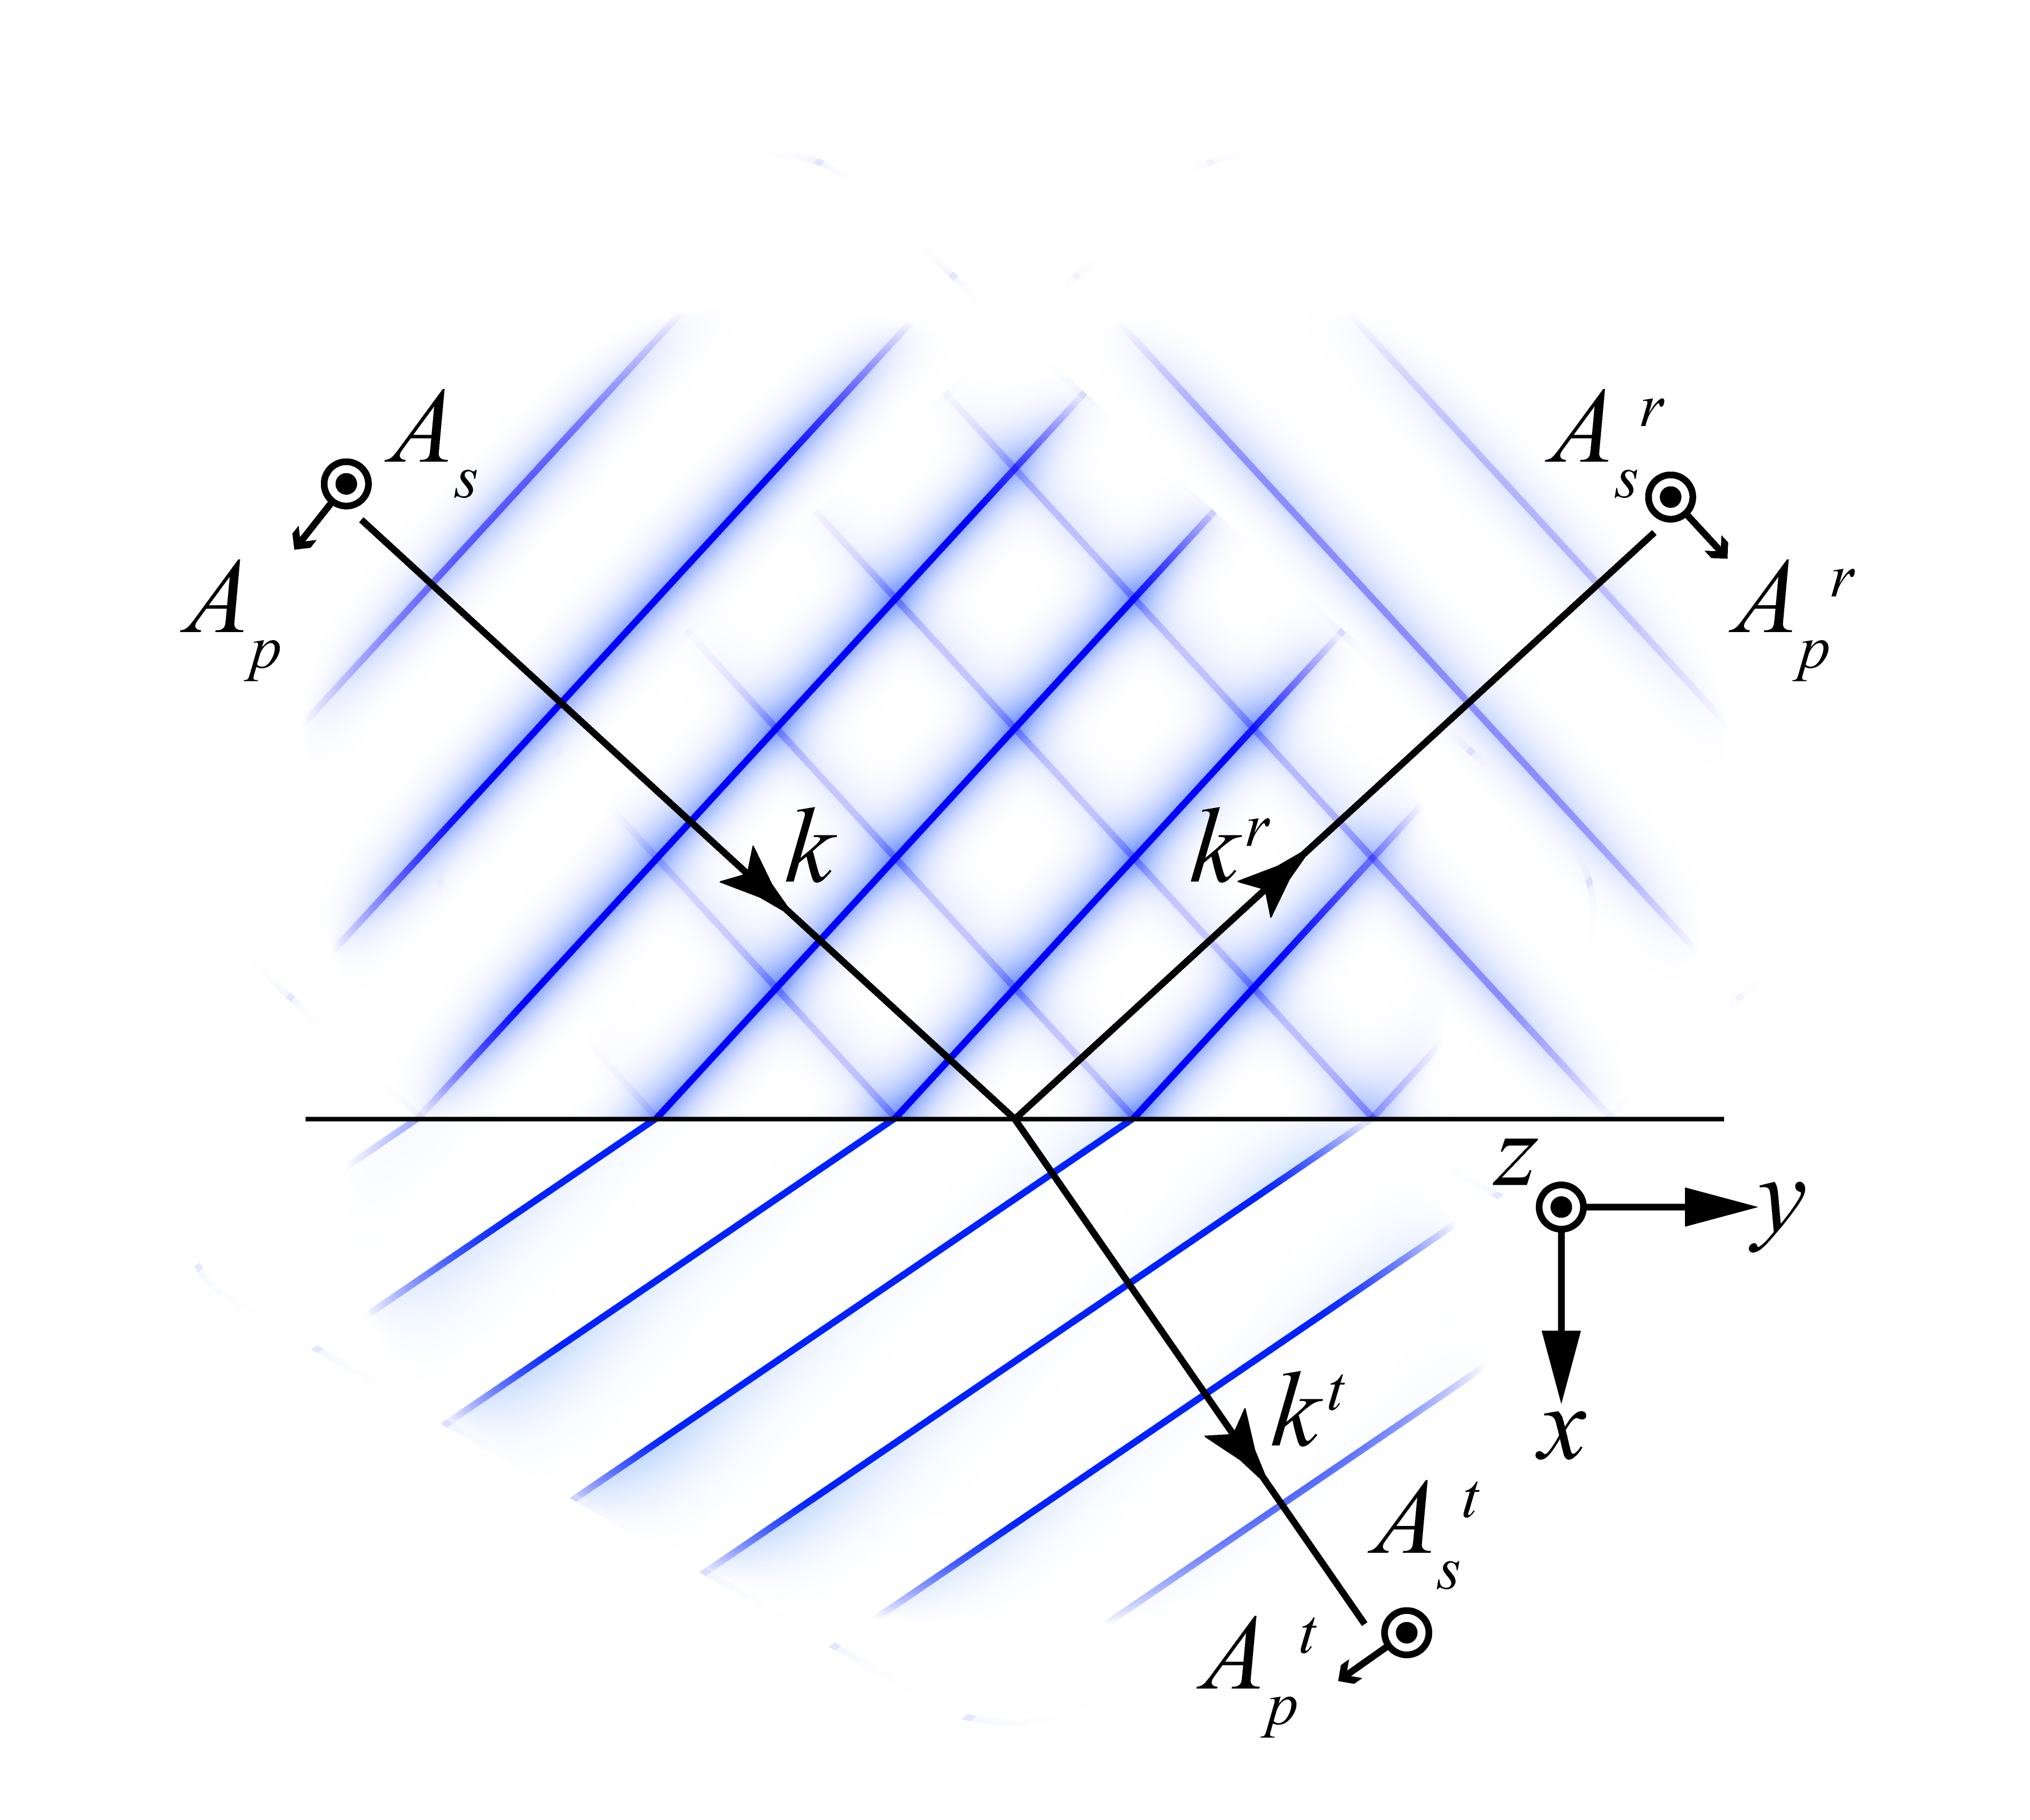
\includegraphics[width=8cm]{image/5-6-4.png}
\caption{界面与两种模式}
\end{wrapfigure}
如图,\,在一个典型的界面上反射与折射的过程中,\,反射光,\,折射光的强度实际上是与入射光的偏振状态有关的.\,这一点在接下来的计算中也可以表明.\,我们按照惯例,\,取两个独立的线偏振为:
\begin{itemize}
	\item \emph{横电波}(TE wave),\,即垂直偏振波(s\footnote{来自德语词senkrecht:\,垂直.}-wave,\,s-polarized wave),\,它的电场方向垂直于主平面\footnote{由入射线与界面法线确定的平面,\,显然,\,出射波与折射波光线方向也在这个平面内.}.\,而磁场方向则在主平面内.
	\item \emph{横磁波}(TM wave),\,即平行偏振波(p\footnote{来自德语(英语)词parallel:\,平行.}-wave,\,p-polarized wave),\,它的电场方向平行与主平面.\,而磁场方向垂直主平面.
\end{itemize}

\npg{-3cm}

它们的正方向如图所示,\,满足\(\bs{A}_s\times\bs{A}_p//\bs{k}\).\,而反射折射系数则定义为在\((0,0,0)\)点处的界面两侧各光振幅比:
\[A_{s,p}=E_{s,p}\ue^{\ui(\bs{k}\cdot \bs{r}-\omega t)}\; ,\; A_{s,p}^r=E_{s,p}^r \ue^{\ui(\bs{k}^r \cdot \bs{r}-\omega^r t)}\; ,\; A_{s,p}^t=E_{s,p}^t \ue^{\ui(\bs{k}^t \cdot \bs{r}-\omega^t t)}\]
\[r_{s,p}=\frac{E_{s,p}^r}{E_{s,p}}\; ,\; t_{s,p}=\frac{E_{s,p}^t}{E_{s,p}}\]

对于$s$-光,\,电磁场在界面两侧切向电场连续,\,切向磁场强度连续\footnote{法向电位移为零.}.\,而对于$p$-光,\,切向也有电场连续,\,法向可以用电位移连续.\,注意到边界条件对任意$t$成立,\,这给出了:
\[\omega=\omega^r=\omega^t\]

也就是折射反射不能改变光的频率,\,也就是颜色.\,从光量子论的角度理解这代表\emph{弹性}(elastic)作用,\,光子的能量将不受改变,\,介质不会以某种共振的方式吸收入射光的能量.\,上式还意味着\(k=\dfrac{\omega}{c/n}=n\dfrac{\omega}{c}=nk_0\propto n\),\,介质内的波矢比同样颜色的真空光要大折射率$n$倍.

而这个边界条件对任意界面$y$坐标也是恒成立的,\,这给出了:
\[k_y=k\sin\theta=k^r\sin\theta^r=k^t\sin\theta^t\]

即折射时平行于界面方向的波矢是不变的.\,光量子论下可以理解为这个方向动量不变,\,没有受到沿平行界面方向的相互作用.\,但注意到$k$与$n$的正比关系,\,将折射方折射率记做$n'$,\,折射角记做$\theta'$我们得到了著名的\emph{斯涅耳定律}(Snell's Law):
\[\theta^r=\theta \quad ;\quad n\sin\theta=n'\sin\theta'\]

再注意到在光学问题中我们一般只讨论透明介质,\,它们磁导率十分接近真空\(\mu\approx \mu_0\),\,在此时实际上\(\dfrac{c}{n}=\dfrac{1}{\sqrt{\varepsilon\mu}}\)给出了\(n=\sqrt{\dfrac{\varepsilon}{\varepsilon_0}}=\sqrt{\varepsilon_r}\).\,而此时实际上电位移振幅就是\(D=\varepsilon E=n^2\varepsilon_0 E\propto n^2 E\)磁感应强度振幅就是\(B=\sqrt{\varepsilon\mu}E=\dfrac{n}{c}E\propto nE\),\,磁场强度$H$与它只差一个真空磁导率$\mu_0$.\,依此我们写出$s$-光与$p$-光的边界条件:
\[E_s+E_s^r=E_s^t\quad ;\quad nE_s\cos\theta-nE_s^r\cos\theta=n'E_s^t\cos\theta'\]
\[E_p\cos\theta-E_p^r\cos\theta=E_p^t\cos\theta'\quad ;\quad n^2E_p\sin\theta+n^2E_p^r\sin\theta=n'^2E_p^t\sin\theta'\]

解之,\,我们得到的则是著名的\emph{菲涅尔公式}(Fresnel's equations):
\[r_s=\frac{n\cos\theta-n'\cos\theta'}{n\cos\theta+n'\cos\theta'}\quad ;\quad t_s=\frac{2n\cos\theta}{n\cos\theta+n'\cos\theta'}\quad ;\quad t_s-r_s=1\]
\[r_p=\frac{n'\cos\theta-n\cos\theta'}{n'\cos\theta+n\cos\theta'}\quad ;\quad t_p=\frac{2n\cos\theta}{n'\cos\theta+n\cos\theta'}\quad ;\quad \frac{n'}{n}t_p-r_p=1\]

都满足:
\[n(1-|r_{s,p}|^2)\cos\theta=n'|t_{s,p}|^2\cos\theta'\]

其中\emph{反射率}(reflectance)与\emph{透射率}(transmittance)分别被定义为:
\[R_{s,p}=|r_{s,p}|^2\quad;\quad T_{s,p}=\frac{n'\cos\theta'}{n\cos\theta}|t_{s,p}|^2\]

透射率与透射振幅系数\(t_{s,p}\)关系前多出来的系数,\,一是由于在介质中能流密度正比于折射率\(I\propto |\bs{E}\times\bs{H}|\propto nE^2\),\,二是折射后方向改变,\,两侧对应光束部分的横截面积也会发生改变.\,下图展示了空气(\(n=1\))与玻璃(\(n=1.5\))界面上的\emph{外入射}(external incidention)与\emph{内入射}(internal incidention)时的情形.
\begin{figure}[H]
\centering
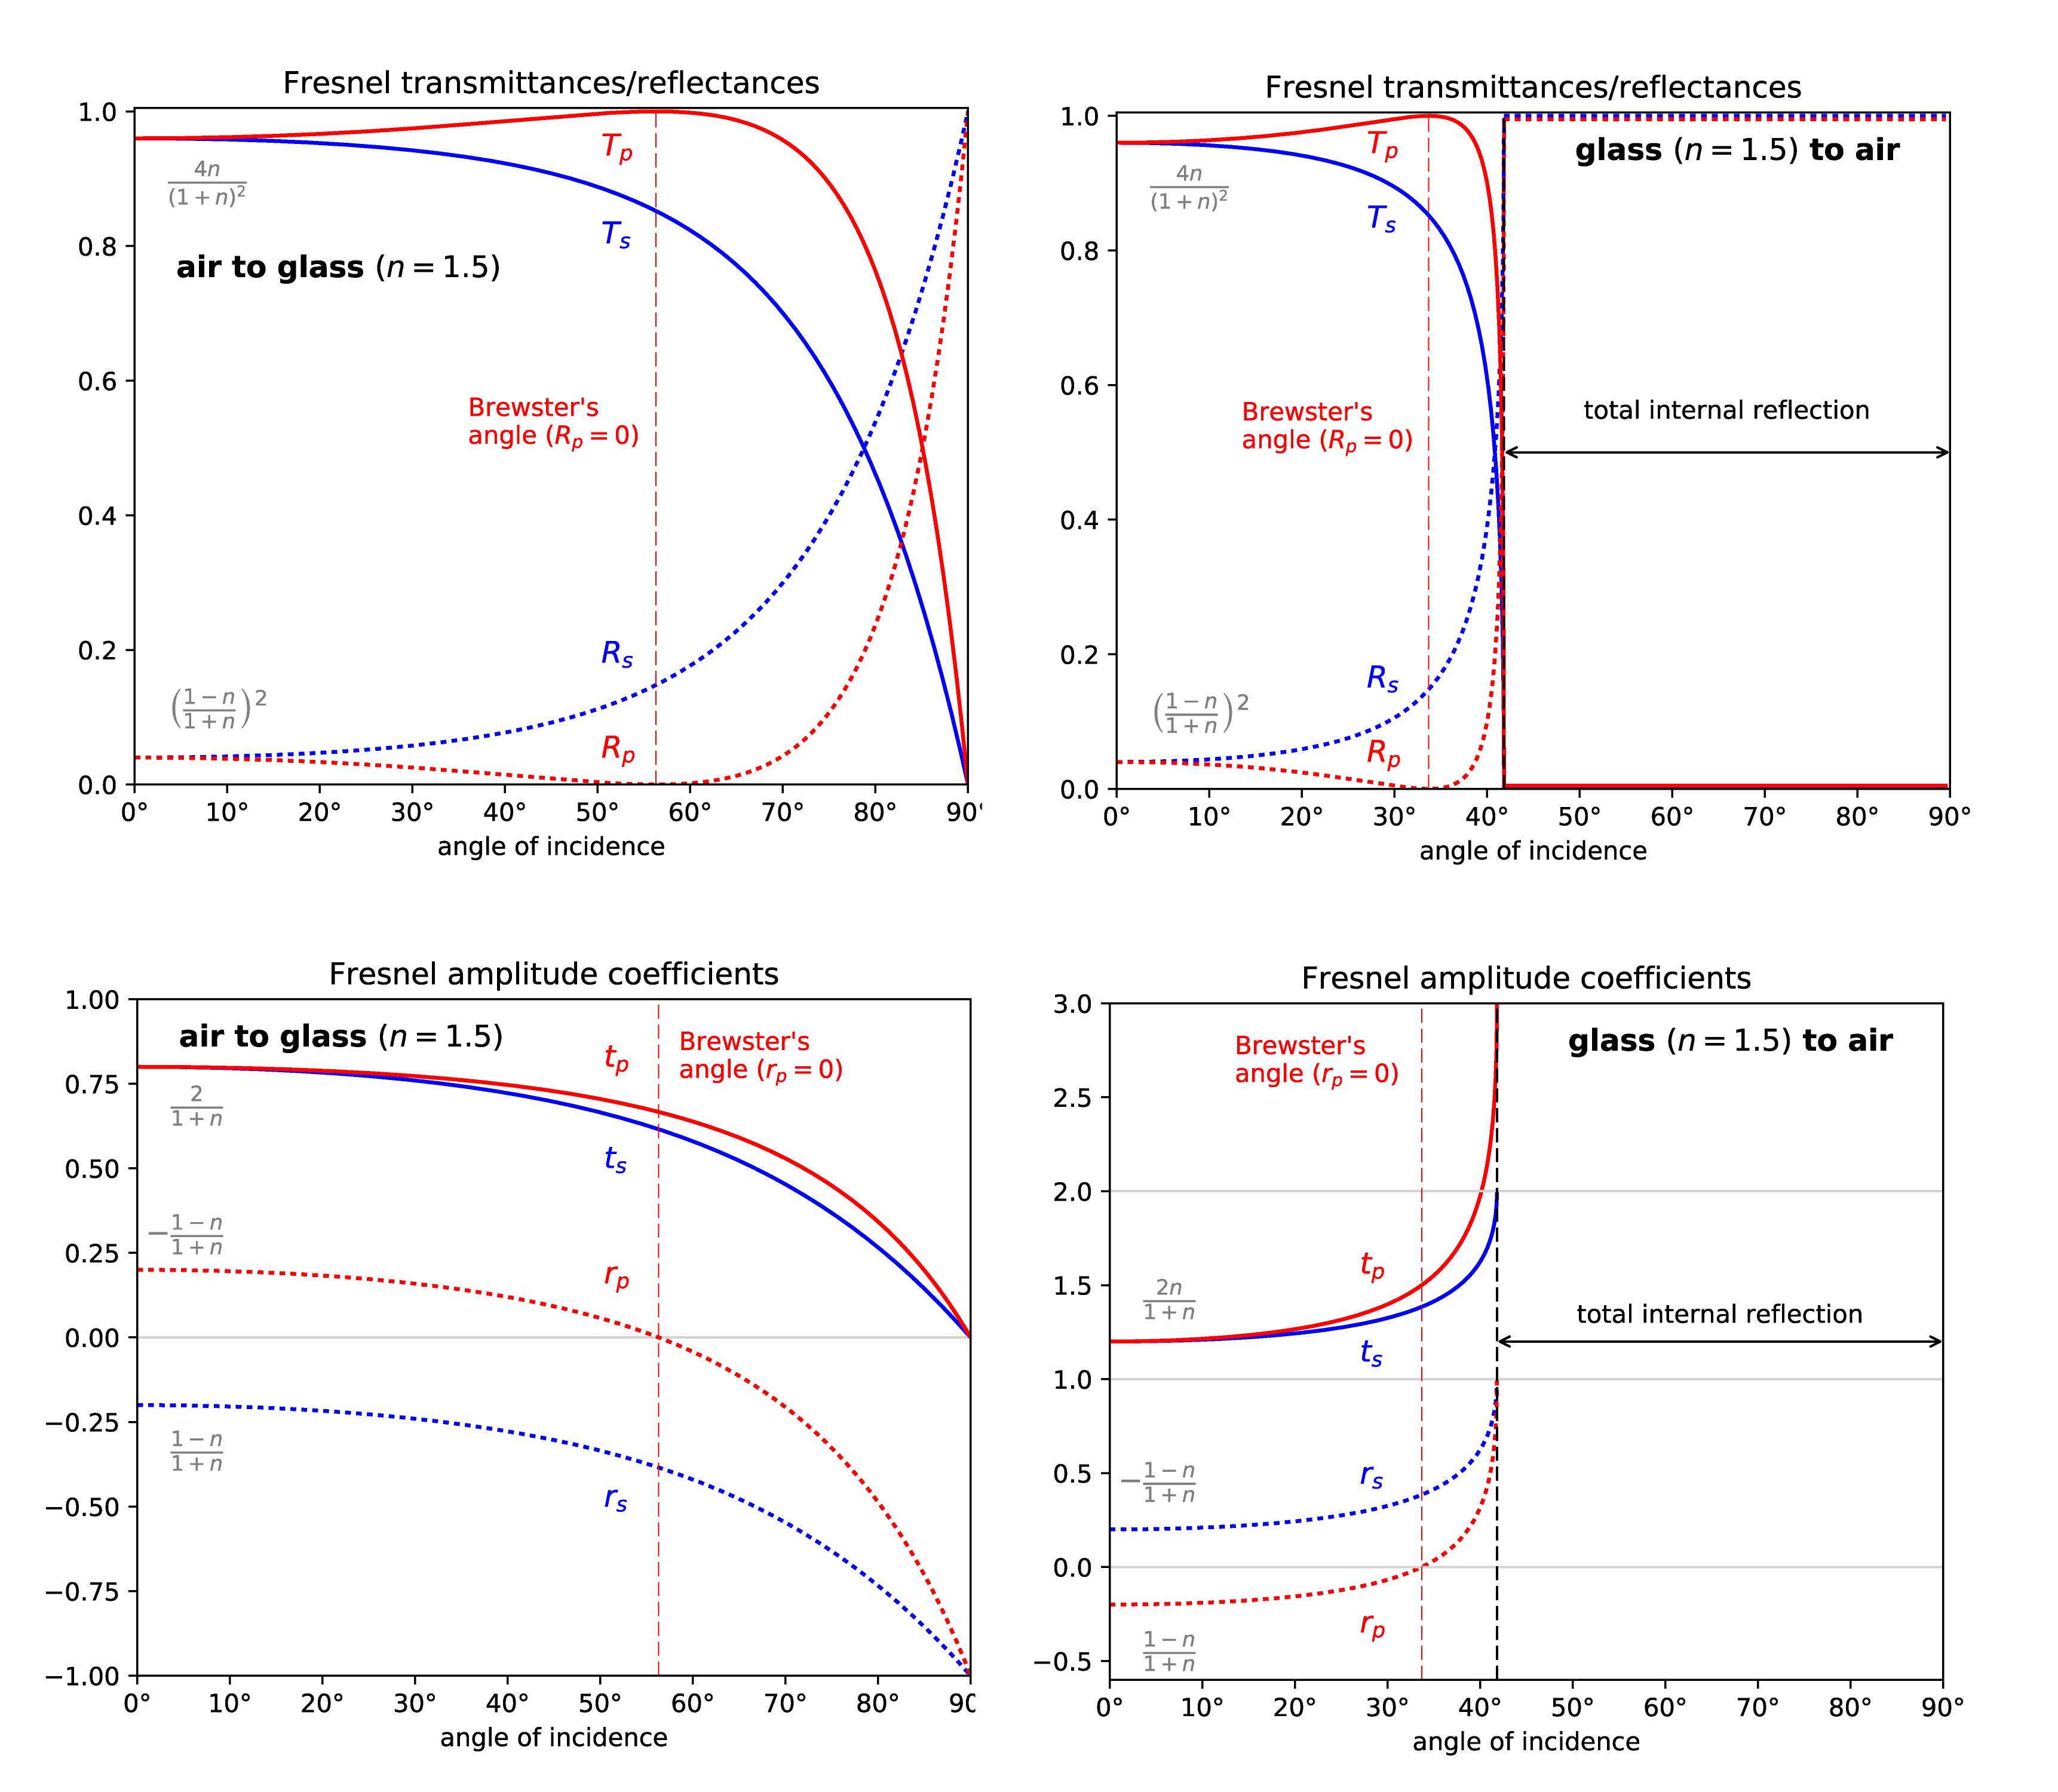
\includegraphics[width=0.8\textwidth]{image/5-6-5.png}
\caption{界面反射与折射}
\end{figure}

有几点值得注意:

\subsubsection{\hei 半波损失发生条件}

当正入射时,\,反射光可以与入射光发生叠加.\,我们关心在$x=0$处,\,也就是界面上的叠加结果.\,当$n'>n$时,\,由上图可见\(r_p>0\)而\(r_s<0\).\,但注意到在此处我们预设的入射反射电场正方向对$p$-光本来也相反而$s$-光相同.\,故事实上都是相干相消.\,发生了\emph{半波损失}(half-wave loss).\,而若$n'<n$时情况恰好相反,\,两种光都是相干相长,\,没有半波损失.

而对于入射角为\(90^\circ\)的掠入射情形,\,观察可知\(r_{s,p}=-1\),\,即反射光完全与入射光交叠区域几乎完全相干相消.\,这个结论对两种偏振模式与两种入射方式均给出了半波损失的结果.

注意透射光几乎在所有情形下都与入射光同相.\,唯一的例外发生在全内反射情况下.\,之后将仔细讨论之.

\subsubsection{\hei 布儒斯特角}

\begin{wrapfigure}[8]{o}[-10pt]{6cm}
\centering
\vspace{-2cm}
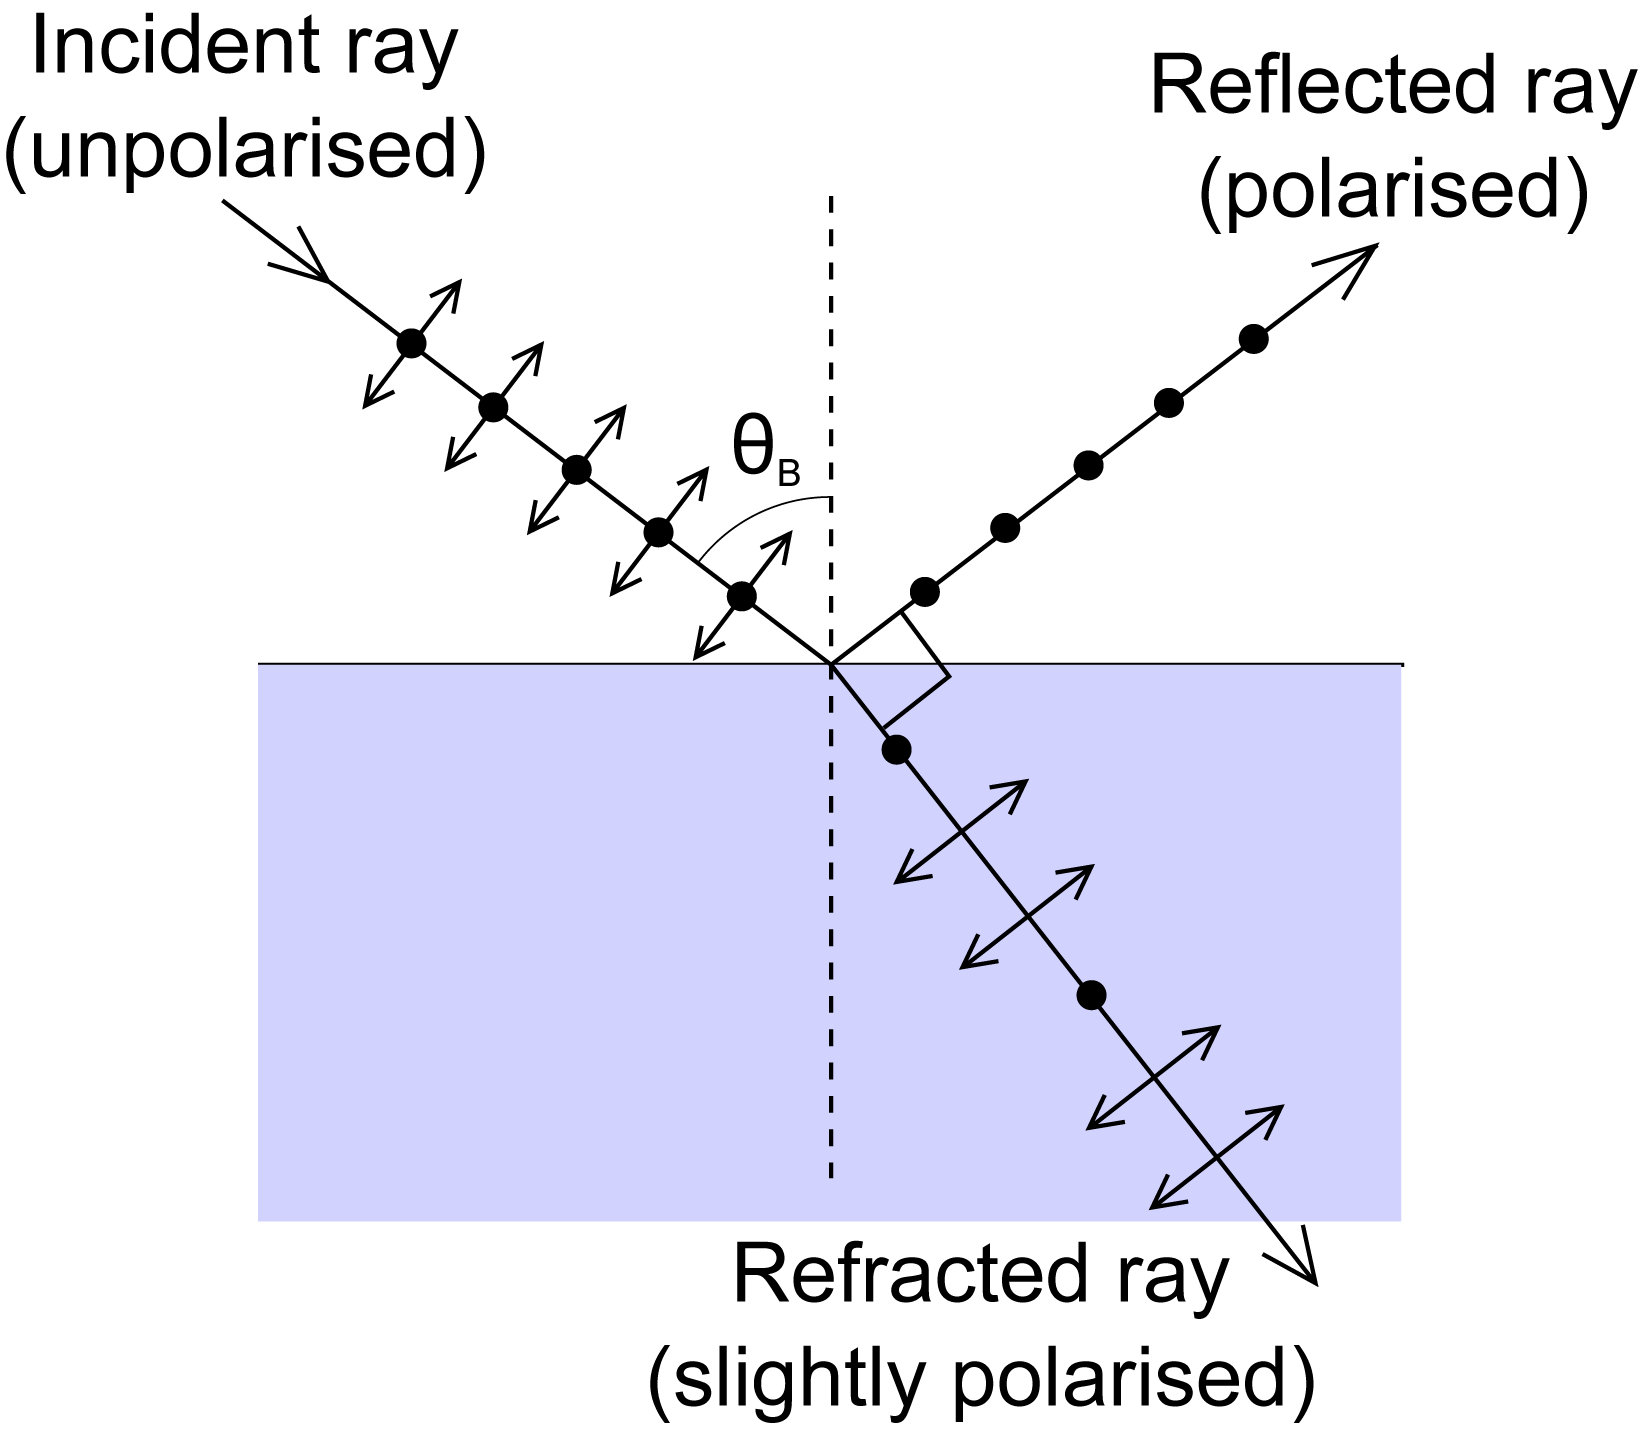
\includegraphics[width=6cm]{image/5-6-6.png}
\caption{布儒斯特角}
\end{wrapfigure}
注意到:
\[r_p=\frac{n'\cos\theta-n\cos\theta'}{n'\cos\theta+n\cos\theta'}=\frac{\sin\theta\cos\theta-\sin\theta'\cos\theta'}{\sin\theta\cos\theta+\sin\theta'\cos\theta'}=\frac{\tan(\theta-\theta')}{\tan(\theta+\theta')}\]

可以发现在\(\theta+\theta'=\dfrac{\pi}{2}\)时\(r_p=0\),\,横电的$p$-光将发生消光的情形.\,这种特殊的情况在内入射与外入射时都可以发生.\,对应的入射角称为\emph{布儒斯特角}(Brewster's angle).\,其原因可以这样理解:\,将入射波变为折射波与反射波实际上是介质电偶极子在电场驱动下振动的集体结果.\,而对于$p$-光,\,反射方向恰恰是介质内电场激发的偶极振动的振动方向.\,按照电磁波的辐射理论,\,这个方向上恰好是辐射强度为零的.\,所以恰好反射波消失.

依照这一种特性制作出来的\emph{布儒斯特窗}(Brewster window)常见于各种气体激光器的内置谐振腔或发射口.\,它将一块透明介质倾斜至布儒斯特角的位置,\,它有效地将$s$-光进行反射,\,而$p$-光没有反射的直接出射,\,使得出射激光一般都是沿p-方向高度偏振的.

\subsubsection{\hei 全内反射与隐失波}

在内入射状态下如果入射角足够大,\,根据斯涅耳定律将无法确定折射角\(\sin\theta'>1\).\,这种情形为\emph{全内反射}(total internal reflection).\,因为接下来的计算可以表明反射系数\(R_{s,p}=1\).\,而实际上此时并不是完全没有折射光场,\,而是折射光场被局域在有光照射的表面区域无法传播开来.

首先,\,折射光场由于边界条件在边界上每个时空点都成立,\,它依然符合:
\[\omega'=\omega\quad ,\,\quad k_y'=k_y=k\sin\theta\]

但此时由于\(x,y\)方向波矢仍然满足\(\displaystyle k_x'^2+k_y'^2=k'^2\),\,而由于入射角足够大使得\(k_y>k'\),\,所以实际上$k_x'$只能成为一个虚数:
\[k_x'=\pm\ui \kappa\quad ;\quad \kappa=\sqrt{k^2\sin^2\theta-k'^2}=\frac{\omega}{c}\sqrt{n^2\sin^2\theta-n'^2}\]

取正号还是取负号呢?\,这实际上取决于我们想研究的问题.\,在此处我们关心\(k_x=+\ui\kappa\)的解.\,这是因为这使得相位因子\(\displaystyle \ue^{\ui k_x x}\)成为衰减因子\(\displaystyle \ue^{- \kappa x}\)而不是正的指数爆炸因子\footnote{这意味着下方的场才是需要关心的而界面上的场仅仅是弱地可以忽略的边缘效应.}.\,这样,\,再将菲涅尔公式中的各个\(\cos\theta\)理解为\(\dfrac{k_x}{k}\),\,我们得到:
\[r_s=\ue^{-2\ui \delta_s}\; ,\; t_s=\frac{2n\cos\theta}{\sqrt{n^2-n'^2}}\ue^{-\ui\delta_s} \quad,\quad\delta_s=\arctan\frac{\sqrt{n^2\sin^2\theta-n'^2}}{n\cos\theta}\]
\[r_s=\ue^{-2\ui \delta_p}\; ,\; t_p=\frac{2nn'}{\sqrt{(n^2-n'^2)(n^2\tan^2\theta-n'^2)}}\ue^{-\ui\delta_p} \quad,\quad\delta_p=\arctan\frac{n\sqrt{n^2\sin^2\theta-n'^2}}{n'^2\cos\theta}\]

\vspace{0.5cm}
\begin{wrapfigure}[13]{o}[-10pt]{7cm}
\centering
\vspace{-1cm}
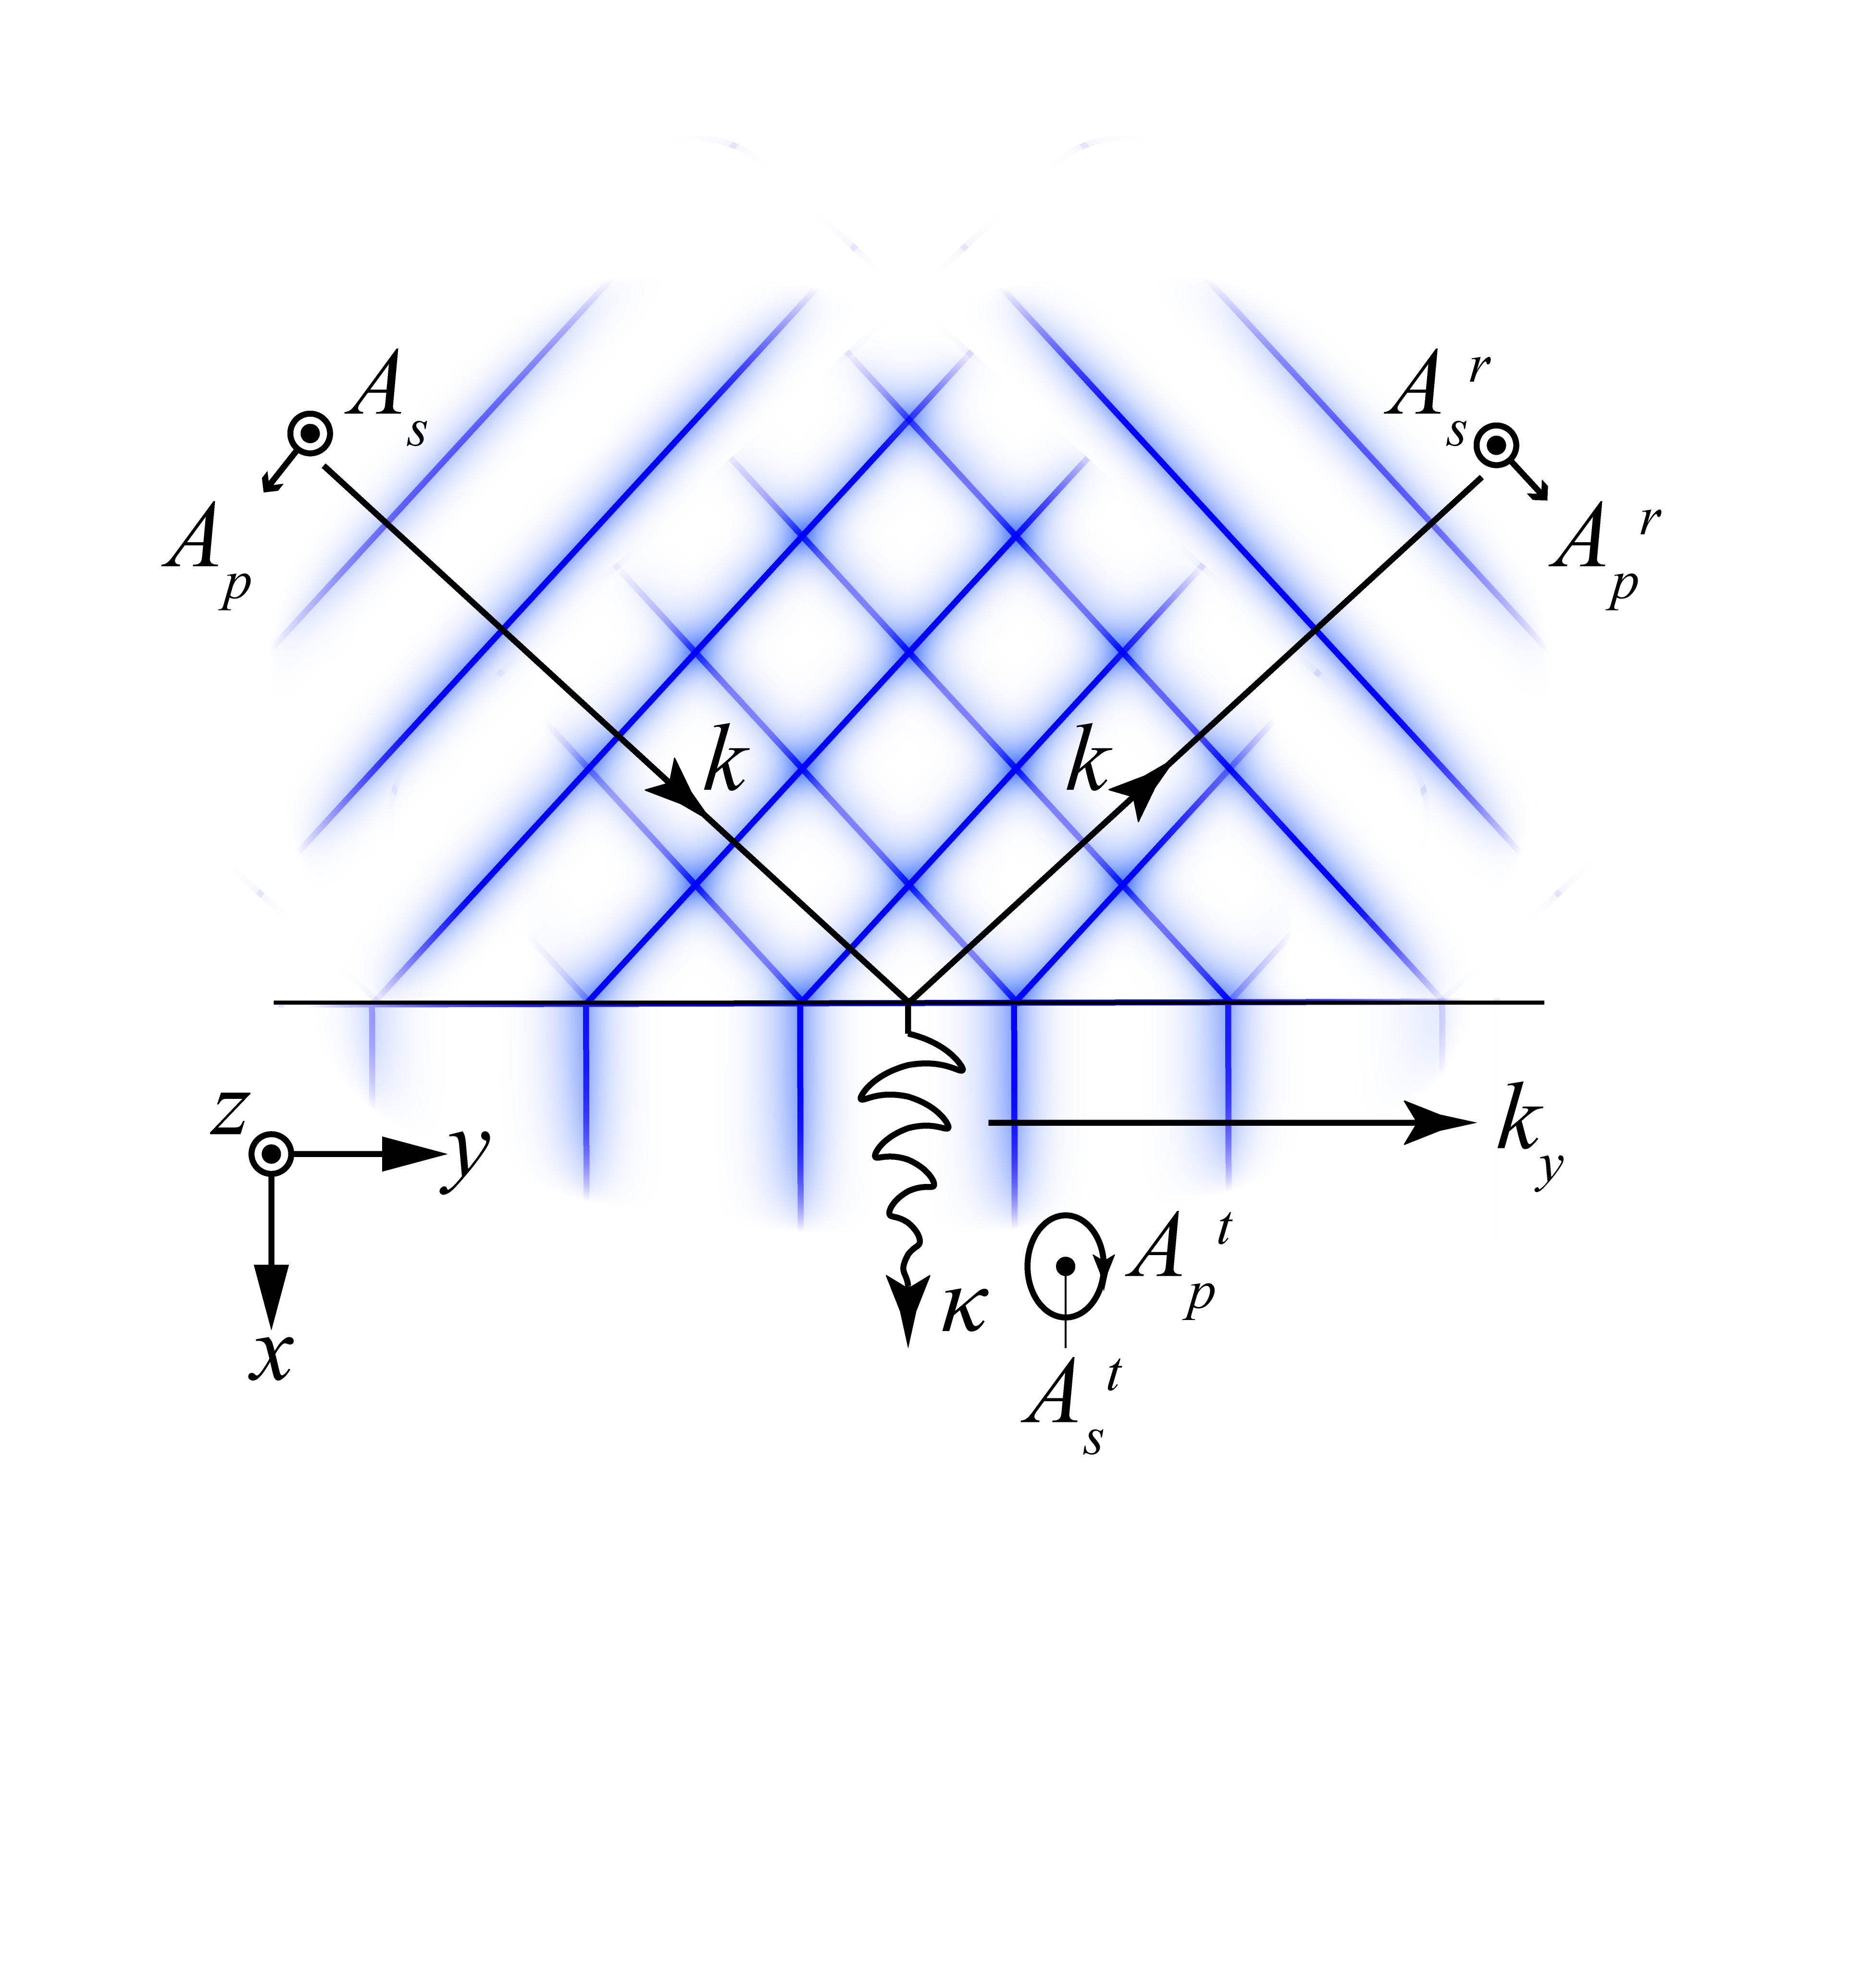
\includegraphics[width=8cm]{image/5-6-7.png}
\vspace{-3cm}
\caption{全内反射与隐失波}
\end{wrapfigure}
可见,\,此时最显著的特点除了反射振幅系数的模为一,\,就是反射波将会与入射波拉开一个非$0$非$\pi$的相位差\(2\delta_s\),\,它随着从临界全内反射到掠入射从$0$不断增加至$\pi$.\,而折射波相位则恰好介于两者之间,\,其振幅在临界全内反射时有极大值,\,此后随着入射角增加而不断减小至零.

更细致的分析可以发现折射光场的$p$-光模式实际上是$x-y$平面上的顺时针椭圆偏振光.\,$s$-光模式则显然还沿垂直平面的$z$方向.\,两者都要在$x$方向上做衰减,\,指数衰减可以表示为:
\[A(x)=A(0)\ue^{-\frac{x}{H}}\]

其中\(\displaystyle H=\frac{1}{\kappa}=\frac{\lambda_0}{2\pi\sqrt{n^2\sin^2\theta-n'^2}}\)称为\emph{衰减深度}(attenuation depth)或\emph{趋肤深度}(skin depth),\,\(\lambda_0\)是真空中的该色光波长.\,由表达式可见其一般$H$就光的波长的数量级.\,正是因为这个原因这种折射波被称为\emph{隐失波}(evanescent field).\,它一定会产生但是由于存在厚度很薄所以难以被探测到.\,如果在隐失波未衰减到零处又重新进入下一层折射角正常的介质,\,那么将会有有限光强的光出射出来.\,这种现象叫做\emph{隐失波耦合}(evanescent wave coupling).\,在光量子论的角度看这实际上是光子的\emph{量子隧穿}(quantum tunnelling)行为.

\npg{-3cm}

\begin{wrapfigure}[12]{o}[-10pt]{7cm}
\centering
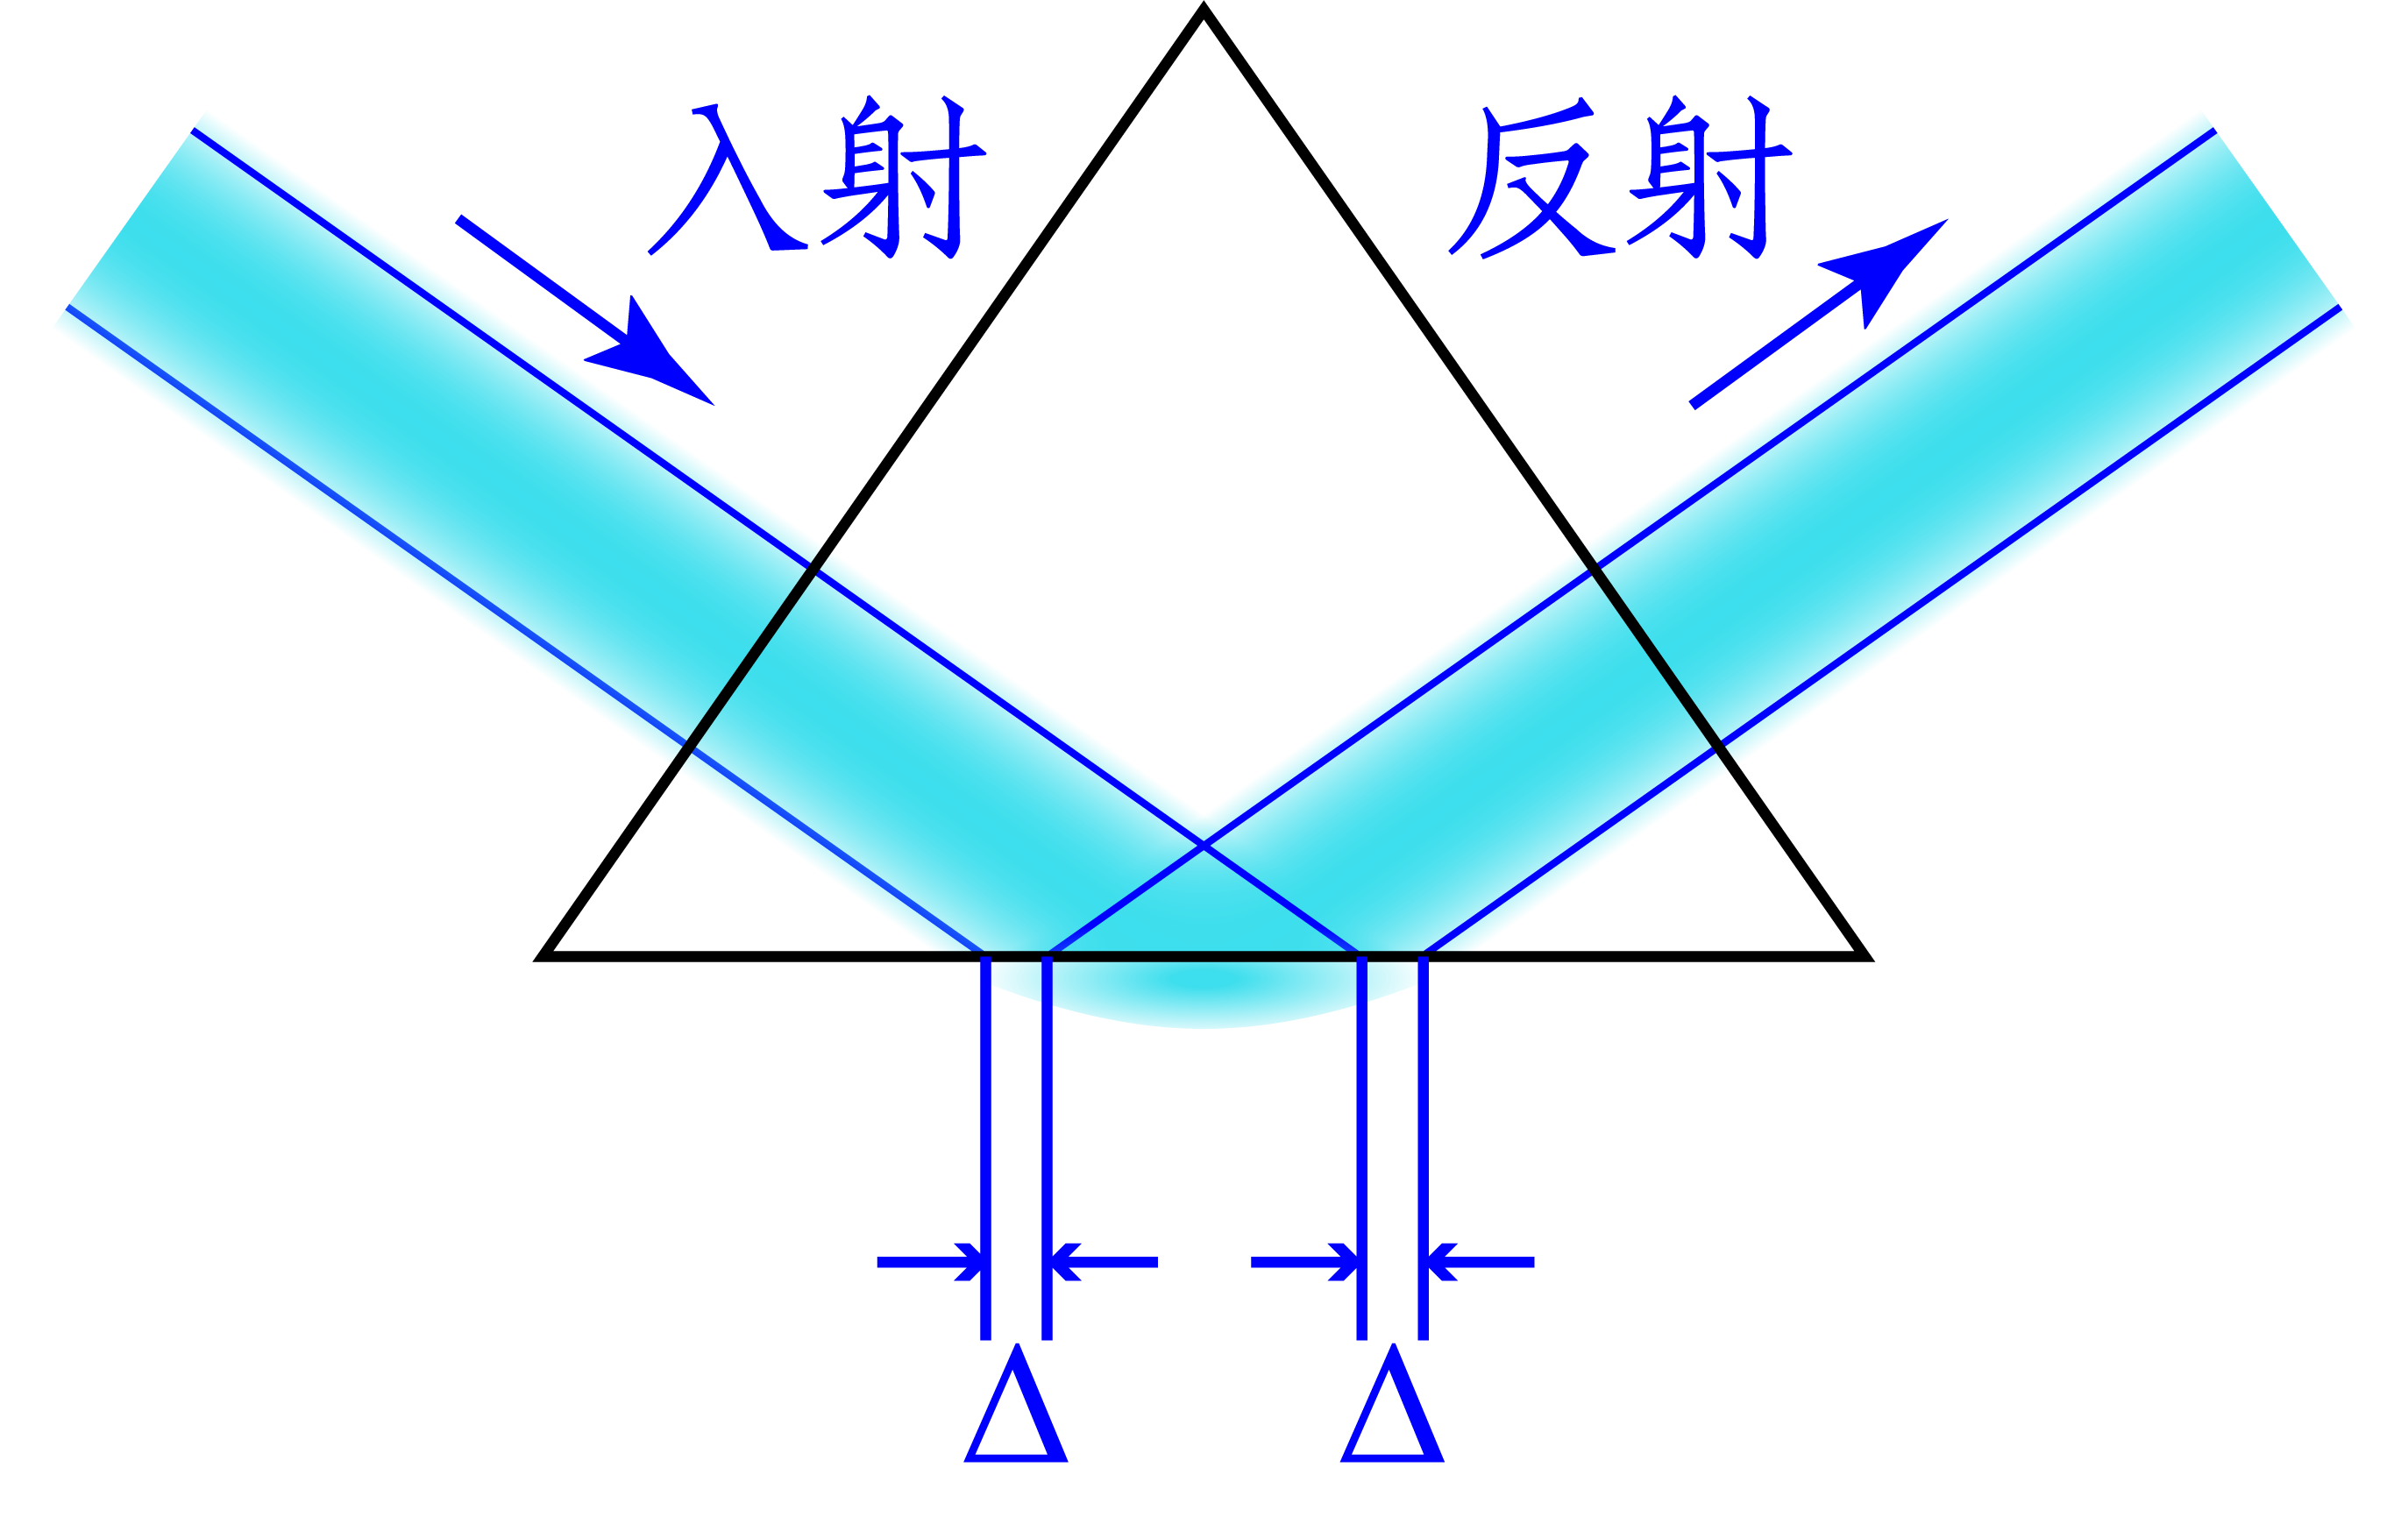
\includegraphics[width=7cm]{image/5-6-8.png}
\caption{Goos-H\"anchen Shift}
\end{wrapfigure}
值得指出,\,如果入射光并不是无限宽的平面波,\,而是可以确定其入射点位置的窄光束,\,而且也不是时刻连续的光,\,而是一个光脉冲,\,那么它的行为体现出更加有意思的结果.\,首先是著名的\emph{古斯-汉森效应}(Goos-H\"anchen effect),\,光脉冲似乎能进入下层介质,\,并在其中传播一段时间,\,随后在另一处离开下层介质出射.\,如图所示,\,这造成的前后光束中心位置的横向移位称为\emph{古斯-汉森位移}(Goos-H\"anschen shift).\,这个位移的计算需要把入射光束看成有一定角度展宽的单色平面波的叠加,\,而在入射点处恰好各个平面波相干相长,\,而光束出射点也是各个出射平面波相干相长的位置,\,不难说明:
\[\Delta_{s,p}=2\frac{\ud \delta_{s,p}}{\ud k_y}=\frac{\lambda\cos^2\delta_{s,p}}{\pi\cos\theta}\cdot\frac{\ud \tan\delta_{s,p}}{\ud \theta}\]

计算可得:
\[\Delta_s=\frac{2H\tan\theta}{n}\quad;\quad \Delta_p=\frac{\Delta_s}{(1+\frac{n^2}{n'^2})\sin^2\theta-1}\]

另一种效应是\emph{英伯特-费多罗夫效应}(Imbert-Fedorov effect).\,如果入射光是两种圆偏振光,\,那么可以证明隐失波场将具有垂直于纸面方向的能流,\,如果入射光是窄光束,\,那么反射光束将在垂直于纸面的方向发生位移,\,这个结果与光的角动量守恒相协调.\,在这里不加论述,\,详情参见光学教材.








\section{光线方程}

\subsection{光线方程与折射定律}
在给定折射率\(n\)随着空间位置连续变化的情况下,\,光将如何进行传播呢?\,把光的传播简化为光线,\,光线垂直于等相位面,\,那么\emph{光线方程}(ray equation)给出了这个问题的答案.\,这个方程写作:
\[\frac{\ud}{\ud s}(n\bs{\tau})=\nabla n\]

\begin{wrapfigure}[14]{o}[-10pt]{6cm}
\centering
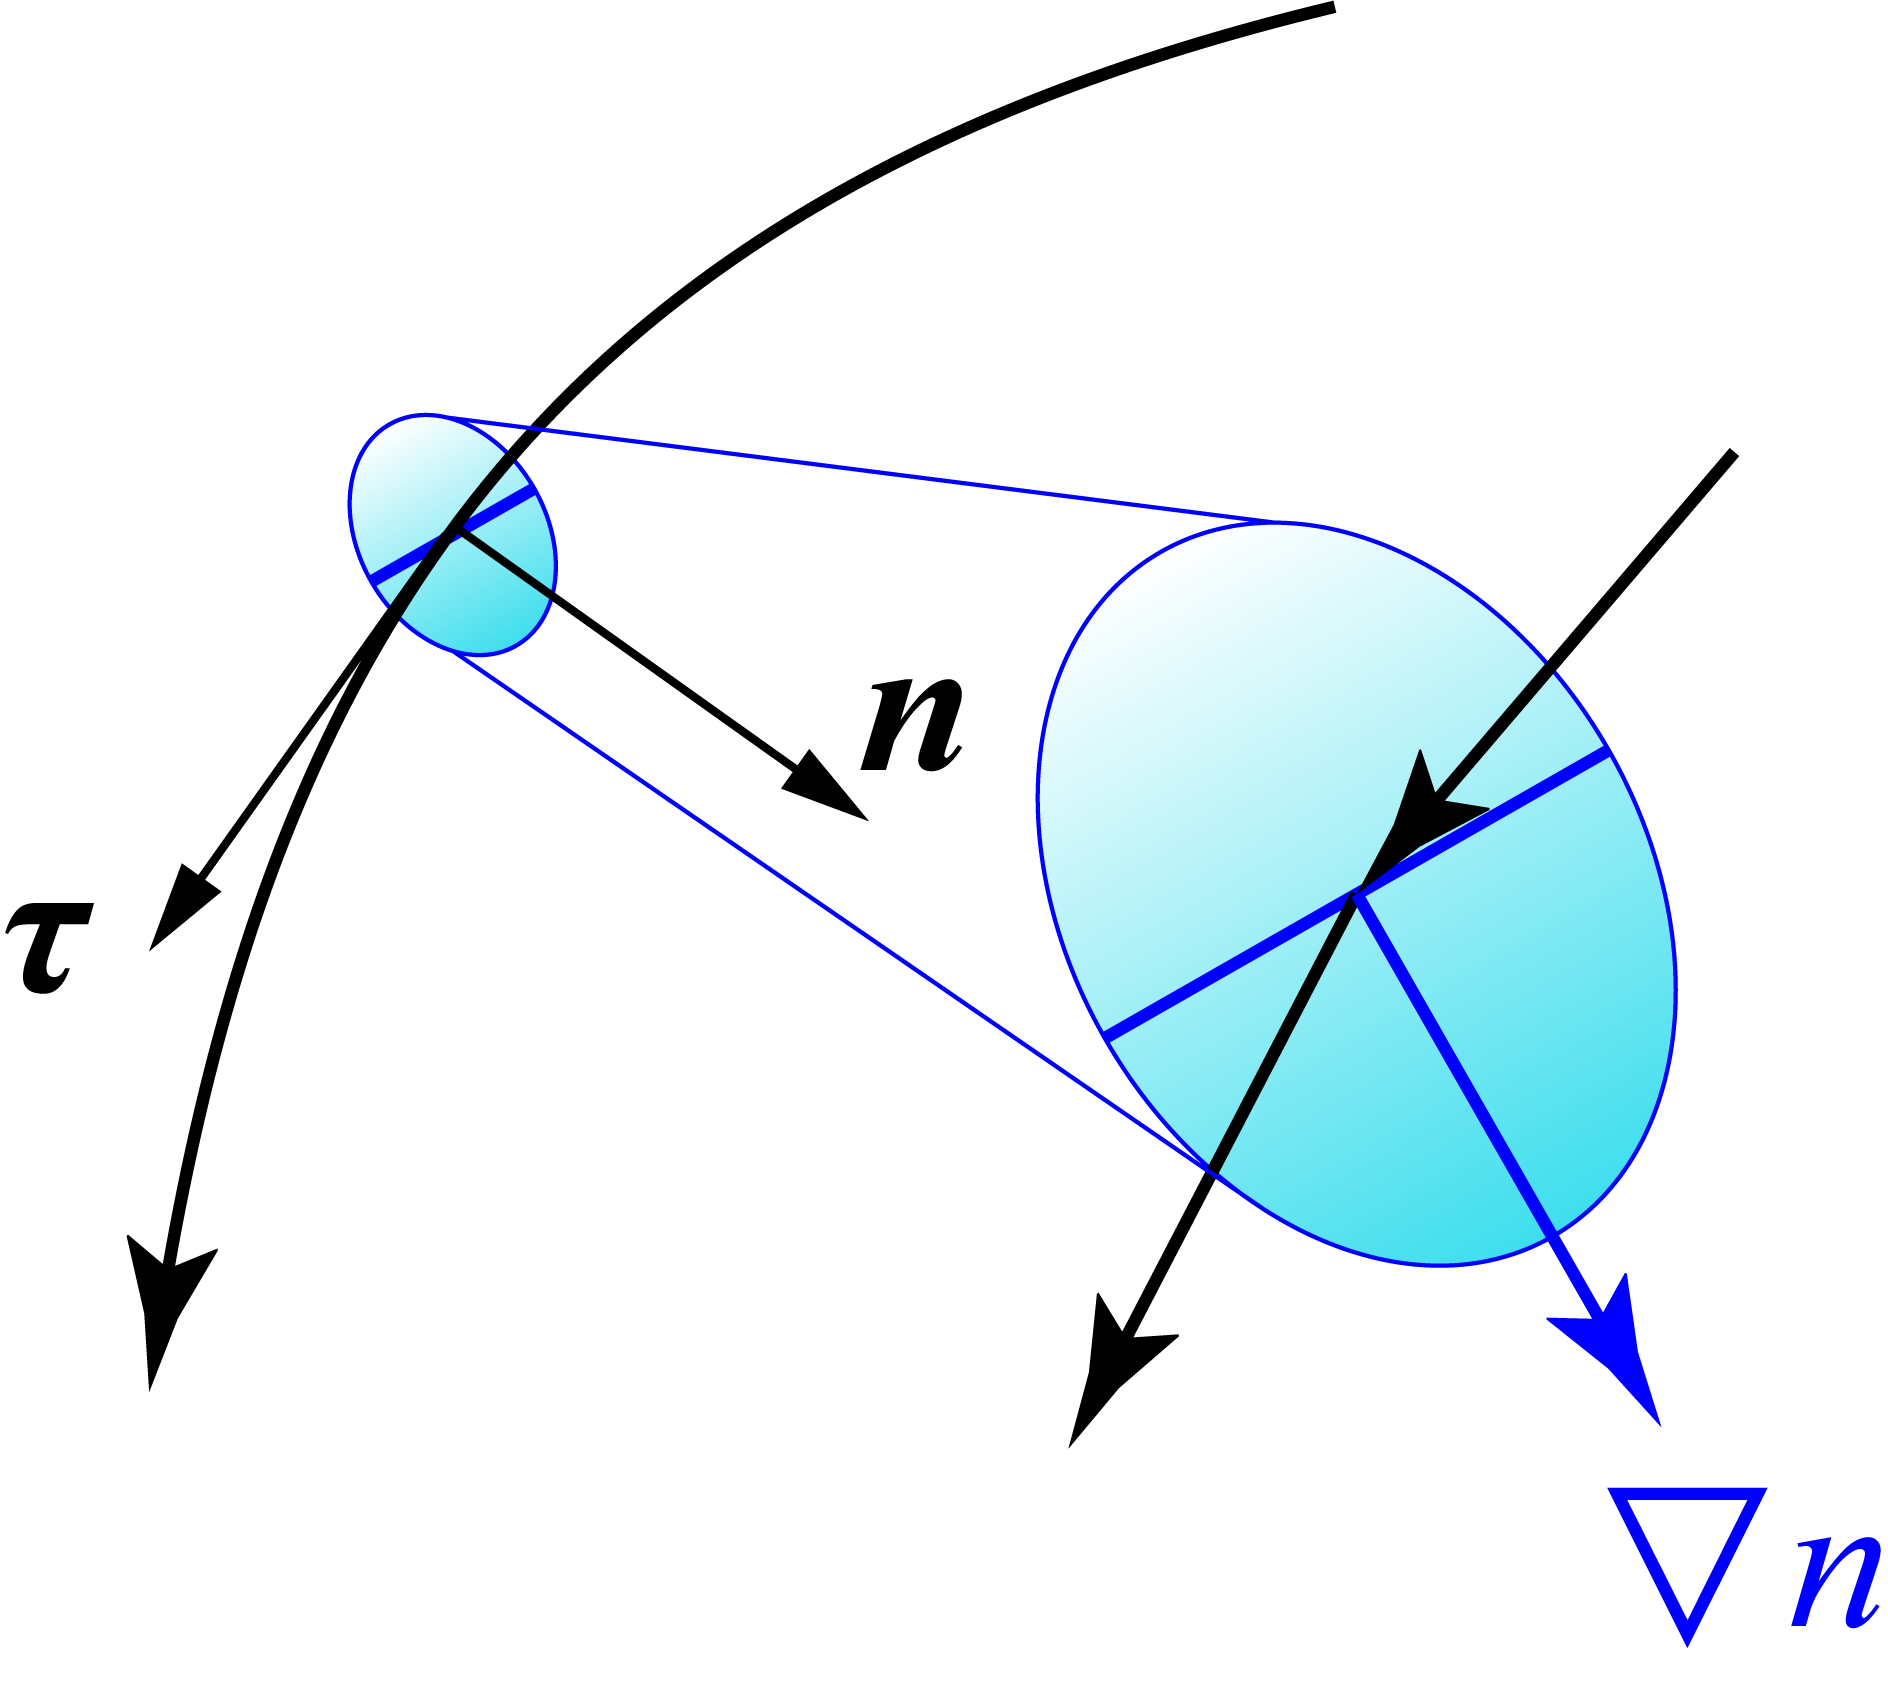
\includegraphics[width=6cm]{image/5-6-9.png}
\caption{光线方程推导}
\end{wrapfigure}
其中\(\ud s\)表示光线经过的路程.\,我们来考虑证明这个式子.\,首先我们先观察上式在法向与切向的两个分量式:
\[(\frac{\ud n}{\ud l})_\tau \bs{\tau}=(\nabla n)_\tau \bs{\tau}\]
\[n\frac{\ud \bs{\tau}}{\ud s}=n\frac{\ud \theta}{\ud s}\bs{n}=(\nabla n)_n \bs{n}\]

那么第一个式子是一个重言式(恒等式),\,而第二个式子则给出了由光线传播方向(给出了切向量\(\bs{\tau}\)与法向量\(\bs{n}\))和局域折射率分布(给出了\(\nabla n\))决定的光线弯曲程度(有曲率\(k=\dfrac{\ud \theta}{\ud s}\)描述).\,是名副其实的能够决定光线传播规律的光线方程.\,事实上,\,如图,\,如果把在该点局域处折射率分布理解为沿\(\nabla n\)的方向进行分层,\,把光线传播方向与局域统一的\(\nabla n\)方向的夹角记为\(\varphi\),\,则当光线走了\(\ud s\)时折射率变化为:
\[\ud n=\nabla n\cdot \ud s \bs{\tau}=|\nabla n|\ud s \cos\varphi\]

由折射定律:
\[\ud(n \sin\varphi)=0\quad \Rightarrow \quad \ud\varphi=-\frac{\sin\varphi\ud n}{n\cos\varphi}=-\frac{|\nabla n|}{n}\ud s\sin\varphi\]

这便是:
\[n\frac{\ud \theta}{\ud s}=n\frac{|\ud \varphi|}{\ud s}=(\nabla n)_n\]

从而给出了光线方程的表达式.

具体的,\,如果研究在二维平面上,\,折射率\(n\)仅仅与\(y\)有关而与\(x\)无关的问题,\,如稳定大气中光线的传播问题,\,此时原光线方程化为:
\[\frac{\ud}{\ud s}(n\sin\theta \bs{e}_x+n\cos\theta \bs{e}_y)=\frac{\ud n}{\ud y}\bs{e}_y\]

注意这时候我们一般取\(\theta\)为光线传播方向与界面法线(\(y\)方向)间的夹角.\,上式一方面意味着
\[n\sin\theta=\mathrm{Const.}\]

这可以看成是两层界面上折射定律的推广,\,它给出了每一个\(y\)处(因而知道\(n\))的光线传播方向,\,从而本质上余下工作只需要解出具体轨迹即可.\,只需解方程:
\[\sin\theta=\frac{1}{\sqrt{1+y'^2}}=\frac{(n_0\sin\theta_0)}{n(y)}\]

其中\((n_0\sin\theta_0)\)是根据初始条件确定的不变量.

\subsection{光力类比}
牛顿提倡光的粒子说,\,他的粒子光学理论中光粒子\footnote{与光子概念有本质区别}运动状态由位置与速度描述,\,而运动由轨迹方程与运动方程描述.\,的确,\,由光线方程可知,\,这是一个定义良好的动力学方程,\,它类似于势场中的牛顿第二定律:
\[\frac{\ud }{\ud t}(mv \bs{\tau})=-\nabla V\]

由粒子的初位置与初速度便可决定论地的给出之后的运动.\,这一种类似性为我们进行光力类比提供了良好的依据.\,然而要注意仍然有一个不同之处:\,光的速度大小不可控.\,在一个典型的光线求解的过程中,\,我们知道初始时刻的光的传播方向即可,\,而传播速度无需给出,\,事实上它也不能被改变,\,因为光速是常数,\,换一个角度理解,\,改变速度就是改变动量与能量,\,那么实际上光子的动量能量改变实际上反应在了光的颜色(频率)上.\,这是与相对论相吻合的一个结论.

那么如何进行光力类比呢?\,还是从以上两个公式的相似性出发,\,我们想象有一个质量为\(m=1\)的粒子在光的真实传播轨迹上运动,\,规定其速度为\(v=n\)\footnote{注意这不是实际光传播的相速度!\,\(v\propto n\)而\(v_g=c/n\propto 1/n\)},\,那么其受力应该为:
\[\bs{F}=\frac{\ud }{\ud t}(mv \bs{\tau})=\frac{\ud }{\ud s/v}(n \bs{\tau})=v\nabla n=n\nabla n=-\nabla(-\frac{n^2}{2})\]

也就是说如果认为粒子是在\(V=-\dfrac{n^2}{2}\)的势场中运动的,\,那么其模仿光线的轨迹与用该处折射率来定标自己的运动速度的做法又恰巧是符合动力学规律的.\,恰巧,\,这个运动的守恒能量:
\[E=T+V=\frac{v^2}{2}-\frac{n^2}{2}=0\]

光粒子的运动只能是能量为零的,\,如果忽略光的色散,\,那么不同频率的光在同一个折射率场中将具有完全相同的传播轨迹,\,实际上没有光粒子运动的``快慢''的说法.

我们总结光力类比法求光线传播问题的大意:

\begin{enumerate}
	\item 明确折射率场分布\(n(\bs{r})\),\,明确光线初始入射位置与方向\(\bs{\tau}_0(\bs{r}_0)\).
	\item 光力类比:\,设置势场\(V(\bs{r})=-\dfrac{n^2}{2}\),\,设置粒子,\,质量为\(1\),\,初始位置\(\bs{r}_0\),\,速度\(\bs{v}_0=n\bs{\tau}_0\).
	\item 求解粒子的运动,\,得出运动轨迹.
	\item 这个轨迹也就是光线的轨迹,\,再由已知的轨迹求解其他问题(如传播时间等).
\end{enumerate}

这种方法往往是方便的,\,它会使得很多我们在力学问题中有明确结论的结果可以直观地呈示出来.\,例如在之前的折射率随\(y\)改变的情形,\,它对应着水平方向平移对称的势场,\,从而有\(x\)方向的动量守恒,\,这就是:
\[n\sin\theta=\mathrm{Const.}\]

同样的道理,\,如果光线在一个球对称的折射率场\(n(r)\)中运动时,\,其轨迹恰好对应有心力场中粒子运动的轨迹.\,例如取:
\[V=-\frac{k}{r}+C\quad\Rightarrow\quad n=n_0\sqrt{\frac{2a}{r}-1}\]

那么这个粒子的运动是在环域\(0<r<2a\)上的椭圆,\,而且计算可以表明改变初始条件,\,其半长轴固定为\(a\),\,保证其轨迹范围不会超过这个环域.

而此时应该有角动量守恒,\,用光线方向与径向夹角\(\theta\)表示则为:
\[nr\sin\theta=L=\mathrm{Const.}\]

\section{费马原理}
\begin{wrapfigure}[14]{o}[-10pt]{6cm}
\centering
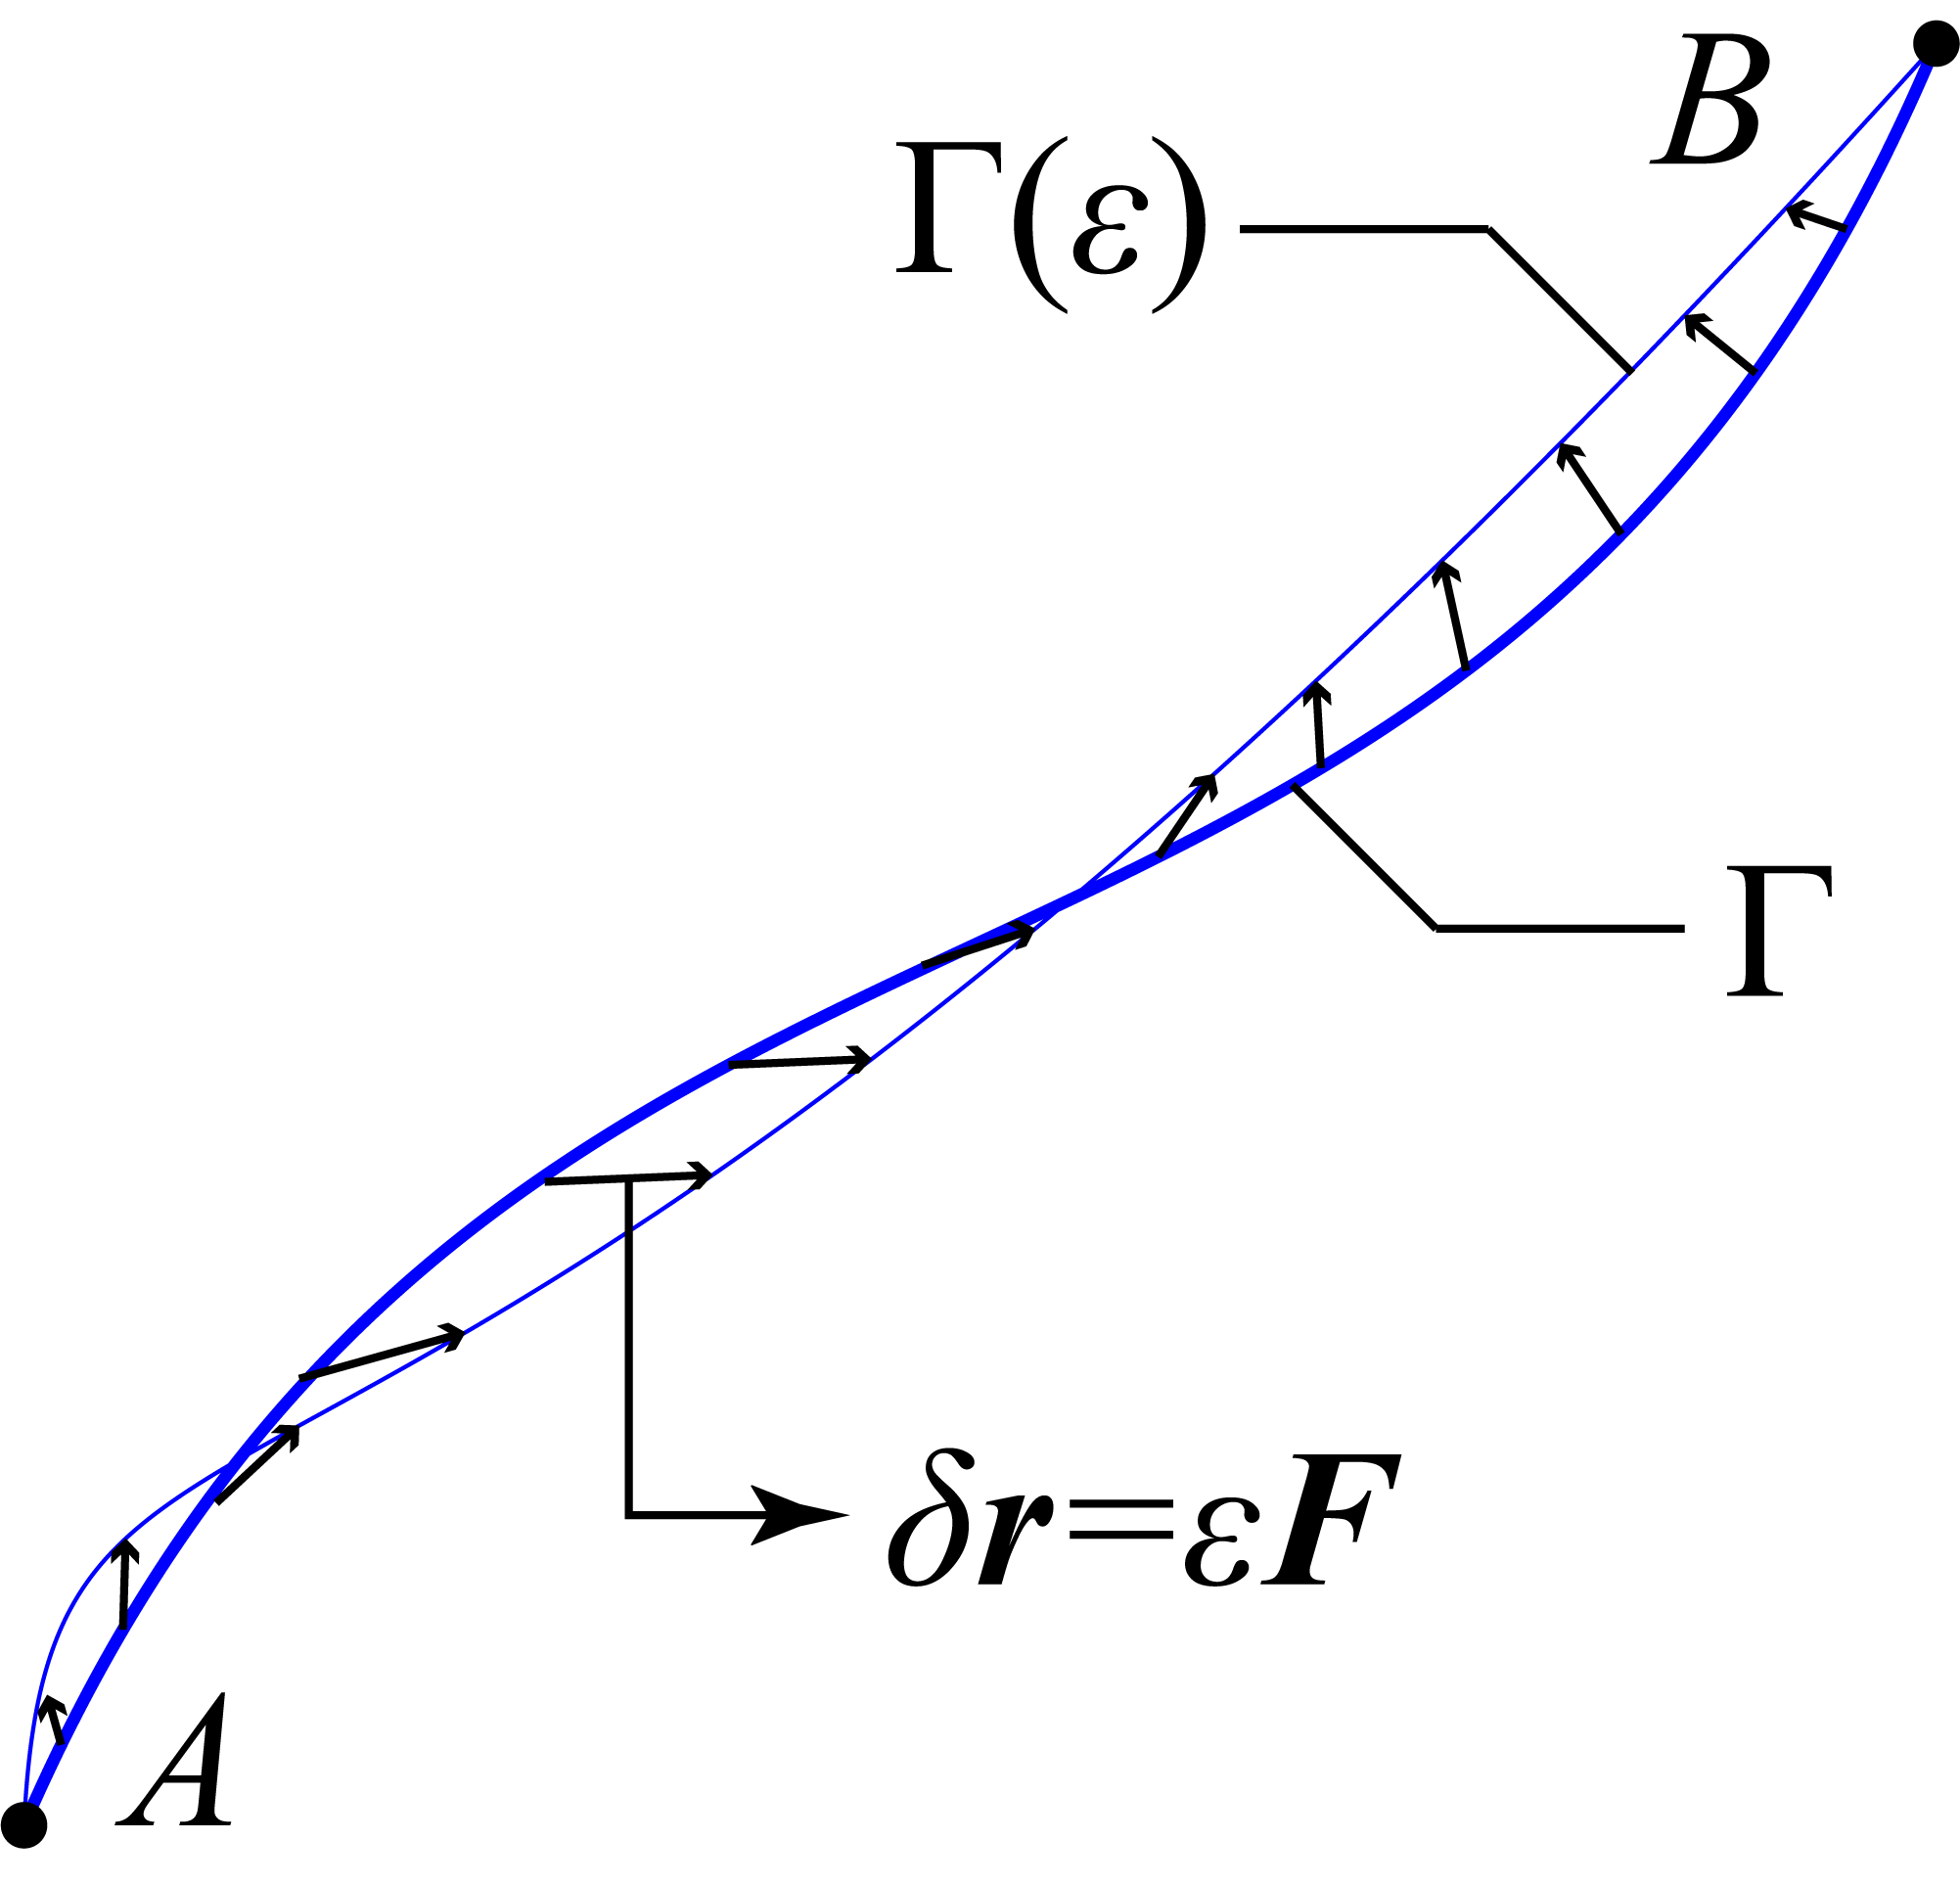
\includegraphics[width=6cm]{image/5-6-10.png}
\caption{光程变分}
\end{wrapfigure}
类似于力学变分原理,\,光线方程的存在也意味着光学的变分原理,\,这个原理即为著名的费马原理:
\[\delta\int_A^B n\ud s=0,\;{\rm if}\;\delta\bs{r}_A=0{\rm \; and \;}\delta\bs{r}_B=0\]

如何理解这个原理呢,\,首先这个折射率对路程的积分称为\emph{光程}(optical path),\,在光力类比下它实际上就是满足能量守恒条件下的相积分:
\[S=\int_{A\xrightarrow{\Gamma} B} n\ud s=\int_{A\xrightarrow{\Gamma} B} \bs{p}\cdot\ud \bs{r}\]

而从\(A\)点到\(B\)点的光传播可以由某种参数方程描述:
\[\Gamma :\quad\bs{r}=\bs{R}(t),\,\bs{R}(t_A)=\bs{r}_A,\,\bs{R}(t_B)=\bs{r}_B\]

而变分的意思是我们另取一种可能的轨迹,\,比如:
\[\Gamma(\epsilon):\quad(\bs{r}+\delta\bs{r})(t)=\bs{R}(t)+\epsilon \bs{F}(t)\]

那么费马原理要求在轨迹端点不变的条件下,\,新的光程关于所有可能的微扰方向\(\bs{F}(t)\),\,关于其微扰强度的一阶导数都要等于零:
\[S(\epsilon)=\int_{A\xrightarrow{\Gamma(\epsilon)} B} n\ud s\quad ;\quad \left.\frac{\ud S(\epsilon)}{\ud \epsilon}\right|_{\epsilon=0}=0\]

这个原理是等价于光线方程的,\,证明这一点需要用到较为专门的矢量分析技巧,\,在此略去.\,用文字一般可以表述为:

\begin{quote}
两点之间光线的实际轨迹,\,是光程取平稳值的路径.
\end{quote}

\begin{wrapfigure}[14]{o}[-10pt]{6cm}
\centering
\includegraphics[width=6cm]{image/5-6-11.png}
\caption{二维鞍点处势取平稳值}
\end{wrapfigure}
其中的``平稳值''的说法,\,既包含了极大,\,也包含了极小,\,还包含了一些复合的情况,\,比如如图,\,我们考虑一个马鞍面上有一个质点在鞍点处于平衡状态,\,那么在一个方向上势能最高,\,另一个方向上势能最低,\,然而该点能平衡,\,因为势能取得了``平稳值''.\,二自由度下已经出现了两个自由度方向微扰后极大极小性质出现差异的情形,\,而光程问题则是在所有可能的轨迹空间中进行无穷多自由度的微扰的问题,\,普遍来说符合之前我们定义的一阶变分为零即可以符合费马原理的条件,\,故冠以``平稳值''的说法.

最后,\,值得指出以上结论都是在波动理论尚未发展到一定程度时的替代性的粒子理论.\,在有了波动理论以后以上两个结论都将得到极为简单的解释.\,我们把变折射率问题中的光的等相位面找到,\,光线即将垂直于等相位面.\,而相位场\footnote{在粒子论里称为\emph{程函}(eikonal)}\(\varphi(\bs{r})\)与光传播方向,\,折射率间关系即为:
\[\nabla\varphi=\bs{k}=k_0 n\bs{\tau}\]

该式两边同时对传播方向取方向导数:
\[\frac{\ud}{\ud s}(\nabla\varphi)=k_0\frac{\ud}{\ud s}(n\bs{\tau})\]

而此式左边,\,在沿传播方向求的导数应该理解为与下一个梯度算符独立的,\,故可以交换顺序:
\[\frac{\ud}{\ud s}(\nabla\varphi)=\nabla(\frac{\ud \varphi}{\ud s})=\nabla{k}=k_0\nabla{n}\]

两式联立便得到光线方程:
\[\frac{\ud}{\ud s}(n\bs{\tau})=\nabla n\]

而费马定理也非常容易理解:\,光程积分:
\[\int n\ud s=\int n\bs{\tau}\cdot \ud \bs{r}=\frac{1}{k_0}\int \nabla \varphi\cdot \ud \bs{r}=\frac{\Delta \varphi}{k_0}\]

所以在光程微扰下只要起点与终点固定,\,光程就不会有改变.

%!TEX root = ../physical-olympics-2.tex
\chapter{光学成像}

\section{傍轴光成像}

\subsection{物与像}
\begin{wrapfigure}[13]{o}[-10pt]{6cm}
\centering
\vspace{-1cm}
\includegraphics[width=6cm]{image/5-7-1.png}
\caption{物与像}
\end{wrapfigure}
成像不是一个平凡的过程.\,延续上一章我们对变折射率问题的讨论,\,现在我们引入所谓\emph{物}(object)的概念,\,它指的是一个点光源\(S\),\,它能够向各种不同的方向发射光线,\,每一个既定的方向则可以根据光线方程求解之后的光线传播.\,这样它所发出的光场构成了物的光场.\,而传播过程中到达的任何一点\(P\),\,满足\(S\)与\(P\)间的真实光线有且只有一条.\,它恰好由费马原理确定.\,但传播过程中可能发生一种奇异的现象,\,就是在空间中另一点\(S'\)处成了\emph{像}(image).\,从光线角度看,\,便是:

\begin{quote}
一定范围内,\,物发出的每一条光线都经过像.
\end{quote}

而根据费马原理,\,真实光线旁边的微扰光线光程对此光线的一阶变分为零,\,但此时有一大组真实光线,\,彼此之间可以连续的过渡,\,我们必然得出:

\begin{quote}
物与像之间的所有真实光线,\,其光程都是相等的.
\end{quote}

以上就是物像之间的\emph{等光程原理}(the principle of equal path length).\,它实际上也是作为了能否成像,\,成像在何处的判据.\,这一个结论也可以依靠干涉理论,\,或者更普遍的,\,光场概率幅的路径积分理论来理解:\,如果两点间光程沿某种路径不是取得极值,\,那么这种情形将会由于存在很多其他类似的路径,\,使得最后在终点处贡献的概率幅相干相消.\,仅仅是在光程取得极值的路径将对最后终点处的概率幅有主要贡献.\,但在物像点间如果存在大量路径其光程完全不变,\,最后像点的概率幅将会非常地大,\,这也就是成像的过程了.

\begin{wrapfigure}[13]{o}[-10pt]{7cm}
\centering
\vspace{0cm}
\includegraphics[width=7cm]{image/5-7-2.png}
\caption{实与虚}
\end{wrapfigure}
以上描述的实际上只是几何光学中的实物与实像的概念.\,在一般的光学系统中,\,光路都是傍轴的.\,即满足\emph{傍轴条件}(paraxial condition):\,有一条中心光线作为\emph{主光轴}(optical axis)参考.\,\emph{光具组}(optical system)把光路分为\emph{物方}(object space)与\emph{像方}(image space).\,两个空间一般都是均匀折射率空间,\,故一般考虑\emph{光锥}(pencil)型光束的传播(就是球面波).\,注意两个空间有可能重合(反射情况).\,这样的光束偏离主光轴的角度满足:
\[\theta\ll 1\]

或者表述为
\[\frac{z}{l}\ll 1\]

其中\(z\)是光路的特征偏离主光轴的距离.\,而\(l\)是光路沿主光轴传播的特征长度.\,如果进入光具组时光束呈现\emph{发散}(diverging)态,\,则说明进入光具组前已有物,\,尽管这一个物有可能也不在真实空间中(如前一次经过光学组后成虚像作为这次的实物),\,也把这样的物称为\emph{实物}(real object).\,它一定位于物方.\,而相反的情况是进入光具组时为\emph{会聚}(converging)光的情况,\,那么物就不可能在物方找到了,\,它位于光具入射面的另一侧(不一定是像方),\,这样的物称为\emph{虚物}(virtual object).\,同理,\,对于像,\,出射光会聚的像位于像方,\,是\emph{实像}(real image),\,而出射光发散,\,像位于像方的另一侧,\,则是\emph{虚像}(virtual image).

\subsection{球对称成像系统与符号法则}
顾名思义,\,球对称成像系统指的是主光轴在一条直线上而整个光具组具有对主光轴的旋转对称性.\,当然实际光锥光路不一定要求关于主光轴对称.\,两种典型的基础光具是折射球面与反射球面.\,如下图所示:
\begin{figure}[H]
\centering
\includegraphics[width=0.9\textwidth]{image/5-7-3.png}
\caption{球面折射与球面反射}
\label{fig5-7-3}
\end{figure}

在球面折射情况\ref{fig5-7-3}下,\,我们先考虑向像方凹的,\,曲率半径为\(R\)的近似球面的傍轴折射成像(作左图).\,各量的符号设定如图,\,\(s\)为\emph{物距}(object distance),\,\(s'\)为\emph{像距}(image distance),\,\(y,\,y'\)则为物,\,像的\emph{高}(height).\,由物像的等光程性,\,应有:
\[f(X,\,Y)=n\sqrt{(X+s)^2+(Y-y)^2}+n'\sqrt{(X-s')^2+(Y-y')^2}={\rm Const.}\]

由于傍轴条件,\,上式中参量\(Y\)是理解为小量变量即可,\,而\(X\)近似为:
\[X=\frac{Y^2}{2R}\]

代入,\,小量近似,\,表示为\(Y\)的二次多项式:
\begin{align*}
f(X,\,Y)	\quad =  &\quad n\sqrt{s^2+y^2}+n'\sqrt{s'^2+y'^2}\\
			   		 &\quad -(\frac{ny}{\sqrt{s^2+y^2}}+\frac{n'y'}{\sqrt{s'^2+y'^2}})Y\\
			   		 &\quad -[\frac{n[(1+s/R)(s^2+y^2)-y^2]}{2(s^2+y^2)^{3/2}}+\frac{n'[(1-s'/R)(s'^2+y'^2)-y'^2]}{2(s'^2+y'^2)^{3/2}}]Y^2
\end{align*}

从而一次项与二次项系数都必须为零.\,由傍轴条件,\,\(s,\,s'\)是\(u,\,v\)的小量.\,从而整理得:
\[\beta=\frac{y'}{y}=-\frac{ns'}{n's}\]
\[\frac{n}{s}+\frac{n'}{s'}=\frac{n'-n}{R}\]

上式给出了成像的\emph{横向放大率}(transverse magnification)与\emph{物像距关系}(object-image distance relation),\,抽象地看,\,在傍轴加二阶近似意义下物方空间每一点都能成像.\,而给定任意物距处的像距与横向放大率,\,就决定了一个光学系统傍轴成像的所有特性.\,以上成像的两个公式的特点是:\,物像距都从球面的顶点开始计算,\,这个点称为\emph{光心}(optical centre).\,这两个公式称为\emph{高斯型公式}(Gaussian formula).\,一般把第二个物像距公式右端的结果定义为\emph{光焦度}(focusing power):
\[\varPhi=\frac{n'-n}{R}\]

其单位是\emph{屈光度}(diopter),\,中文简称``度''.\,\(1{\rm D}=1{\rm m}^{-1}\).

\begin{wrapfigure}[11]{o}[-10pt]{8cm}
\centering
\vspace{0cm}
\includegraphics[width=8cm]{image/5-7-4.png}
\caption{焦点}
\end{wrapfigure}
当物距和像距取特殊值时会出现另一个趋于正负无穷,\,而对应的物像高也趋于正负无穷的情形,\,此时意味着入射,\,出射光成为了\emph{平行光}(collimated light).\,这些特殊的物像距称为\emph{焦距}(focal length),\,而对应的主光轴上的点称为\emph{焦点}(focus).\,物方焦距与像方焦距就分别为:
\[f=\frac{n}{\varPhi}=\frac{nR}{n'-n}\quad ;\quad f'=\frac{n'}{\varPhi}=\frac{n'R}{n'-n}\]

自然地有:
\[f:f'=n:n'\]

通过引入两个焦距我们可以把成像公式写作:
\[\frac{f}{s}+\frac{f'}{s'}=1\quad ;\quad \beta=-\frac{fs'}{f's}\]

实际上,\,\(n,\,n'\)都不是通过这个折射成像系统可以测量的量,\,而两个长度量纲的\(f,\,f'\)代表了这个系统成像的所有特征.

为了更直观地反应物像距指尖关系的特性,\,一般把顺光传播方向,\,物到物方焦点的距离记为另一种物距\(x=s-f\),\,而像方焦点到像的距离记为另一种像距\(x'=s'-f'\).\,那么代入高斯型公式化简可得:
\[xx'=ff'\]
\[\beta=-\frac{f}{x}=-\frac{x'}{f'}\]

以上两个公式更为精简,\,称为\emph{牛顿型公式}(Newtonian formula).\,图像也更加清晰:\,物像距恰好是一个反比关系.\,而横向放大率取决于物离物方焦点有多近,\,也等效于像离像方焦点有多远.\,运用起来往往更加方便.\,仔细观察还会发现,\,仅需\(ff'\)作为整体的大小实际上已经确定了物像距的关系.\,但如果要求的是横向放大率,\,\(f,\,f'\)各自取多少就是必要的了.\,也就是说不仅需要知道两个焦点的位置,\,还得已知光心离各自有多远.

对于\ref{fig5-7-3}右图的球面反射镜,\,只需要把两个焦距定为
\[f=f'=\frac{R}{2}\]

那么高斯型公式与牛顿型公式都以完全一样的形式适用,\,只需注意此时的主光轴正方向在反射时发生了反转,\,物像距的定义会产生相应的改变,\,参照图理解即可.

当我们考虑不同的球面凹凸性,\,不同的折射率分布,\,不同的物像实虚性时显然不希望每次都重新进行推导,\,而是希望我们之前推出的结论具有普适性.\,那么实际上之前我们涉及的每个量都可以有正负(折射率除外).\,约定不同量的正负性的方法称为\emph{符号法则}(sign convention).\,本书介绍一下符号法则:

\begin{enumerate}
	\item 光具球面曲率半径:\,{\hei 出射方看,\,凹正凸负.}\,出射方也就是单次成像的像方,\,如果曲率中心位于这一侧,\,那么曲率半径计为正.\,如果在另一侧,\,计为负.
	\item 物像距,\,焦距:\,{\hei 实正虚负.}\,如果是物点发出的发散光沿主光轴正向传播到物距的零点处则为实物,\,物距计正(实物).\,如果是会聚光传播到物距零点处还未到达物点,\,则物距计负(虚物).\,同理,\,像距零点处出射会聚光可以沿主光轴传播形成像点,\,像距计正(实像).\,若像距零点处出射发散光,\,像点可以认为应在之前形成,\,像距计负(虚像).\,物方焦距是使像距趋于无穷的特殊物距.\,像方焦距是使物距趋于无穷的特殊像距.
	\item 物像高:\,{\hei 上正下负.}\,不管任何情形,\,都规定主光轴的一侧高度大于零,\,一侧小于零.\,也就是把与这个方向垂直的轴上坐标定义为高度.\,如果把主光轴理解为水平方向,\,一般上半空间物,\,像高为正,\,下半空间物像高为负.
	\item 光线的倾角:\,{\hei 增正减负.}\,有时候我们不仅关心物像点间的对应关系,\,也关心一根光线与另一根光线的对应关系.\,而实际上相互对应的光线不仅是物方入射光线与像方出射光线的关系,\,由于每一点某能成像,\,两条线上的点也是一一对应的物像点.\,此时光线的角度被定义为沿传播方向单位长度所增加的物或像高.\,如果光线从下往上传播,\,角度为正,\,从上往下则角度为负.
\end{enumerate}

我们之前推出来的,\,针对于球面折射,\,反射的公式自然是在以上符号法则下普适的.\,同样的道理也适用于之后所有情况下提出的公式.\,而且不失一般性地,\,高斯型公式与牛顿型公式其实是对任意球对称成像系统傍轴适用的.\,推广到非傍轴情形便是下一节讨论的理想成像系统.

\begin{wrapfigure}[11]{o}[-10pt]{8cm}
\centering
\vspace{0cm}
\includegraphics[width=8cm]{image/5-7-5.png}
\caption{薄透镜}
\end{wrapfigure}
我们接着讨论\emph{薄透镜}(thin lens)模型.\,这是一个两次成像的过程,\,第一次成像的像方零像距点,\,第二次成像的物方零物距点恰好重合在透镜的光心位置.\,从而有:
\[\frac{n}{s}+\frac{n_L}{s_1^\prime}=\frac{n_L-n}{R}\quad ;\quad \beta_1=-\frac{ns_1'}{n_L s}\]
\[\frac{n_L}{s_2}+\frac{n'}{s'}=\frac{n'-n_L}{-R'}\quad ;\quad \beta_2=-\frac{n_L s'}{n's_2}\]

注意在第二个公式中\(R'\)是在右表面凸是取正的曲率半径(以双凸透镜为正),\,它与我们既定的符号法则相反,\,故在照抄公式时在分母加以符号以示区别.\,再有上讨论的两个物像距参考关系:
\[s_1'+s_2=0\]

消去中间的物像距,\,得到:
\[\frac{n}{s}+\frac{n'}{s'}=\frac{n_L-n}{R}+\frac{n_L-n'}{R'}\quad ;\quad \beta=-\frac{ns'}{n's}\]

这说明把两次成像的密接的结果是光焦度的直接相加:
\[\varPhi=\varPhi_1+\varPhi_2\]

而除此以外余下公式都没有变化:
\[f=\frac{n}{\varPhi}\quad;\quad f'=\frac{n'}{\varPhi}\]
\[\frac{f}{s}+\frac{f'}{s'}=1\quad;\quad \beta=-\frac{fs'}{f's}\]

这几个规律也适用于密接的透镜组.\,任何发散和会聚光的能力直接用光焦度评价,\,密接时这些规律都直接叠加.

\subsection{光具组成像}
\begin{wrapfigure}[12]{o}[-10pt]{8cm}
\centering
\vspace{0cm}
\includegraphics[width=8cm]{image/5-7-6.png}
\caption{透镜组}
\end{wrapfigure}
如图,\,如果考虑\emph{厚透镜}(thick lens)模型,\,或者更普遍地讨论两个薄透镜相隔一定距离放置的情况.\,那么一般把前透镜像方焦点到后透镜物方焦点的以传播方向为正的距离即为\emph{光学距离}(optical distance).\,即\(\varDelta=\overline{F_1' F_2}\),\,两透镜间距离:
\[d=f_1'+f_2+\Delta\]

上图的\(\varDelta\)实际上取负,\,事实上当\(\varDelta=-f_1'-f_2\)时变为密接的情形,\,而\(\varDelta\)增大也代表着\(d\)增大.\,我们写出此时的成像物像距公式:
\[\frac{n}{s}+\frac{n''}{s_1'}=\varPhi_1\]
\[\frac{n''}{s_2}+\frac{n'}{s'}=\varPhi_2\]
\[s_1'+s_2=d=\frac{n''}{\varPhi_1}+\frac{n''}{\varPhi_2}+\varDelta\]
得到:
\[(s-f_1-\frac{f_1f_1'}{\varDelta})(s'-f_2'-\frac{f_2f_2'}{\varDelta})=\frac{f_1f_1'f_2f_2'}{\varDelta^2}\]

上式即成像公式的牛顿形式.\,而由牛顿型的放大率公式:
\[\beta=(-\frac{f_1}{s-f_1})(-\frac{s'-f_2'}{f_2'})\]

代入上式可得:
\[\beta=-\frac{-\frac{f_1f_2}{\varDelta}}{s-f_1-\frac{f_1f_1'}{\varDelta}}=-\frac{s'-f_2'-\frac{f_2f_2'}{\varDelta}}{-\frac{f_1'f_2'}{\varDelta}}\]

从中可以发现,\,这个成像公式恰恰等价于一个物像距的零点不位于两个透镜光心.\,而两侧的焦点也不与原来的焦点重合的成像系统,\,仍然有其焦距为:
\[f=\overline{FH}=-\frac{f_1f_2}{\varDelta}\;,\; f'=\overline{H'F'}=-\frac{f_1'f_2'}{\varDelta}\quad ;\quad f:f'=n:n'\]

而各个特征点位移为:
\[\delta_F=\overline{F_1F}=-\frac{f_1f_1'}{\varDelta}\quad;\quad \delta_F'=\overline{F'F_2'}==-\frac{f_2f_2'}{\varDelta}\]
\[\delta_H=\overline{O_1H}=-\frac{f_1d }{\varDelta}\quad;\quad \delta_H'=\overline{H'O_2}=-\frac{f_2' d}{\varDelta}\]

其中\(H\)被称作等效光学系统的物方主点,\,\(H'\)被称作等效光学系统的像方主点.以上公式的理解中如果\(\varDelta<0\),\,那么各个量就都是正的.\,图画的正是这个情况.\,此时的成像规律,\,可以认为是在\(H\)处具有光焦度为\(\varPhi=-\dfrac{n''\varDelta}{f_1'f_2}\)的透镜,\,再把其直接成像的结果进行一个平移,\,平移距离即为两个主点间距\(\overline{HH'}\).\,正是因为这个原因,\,考虑多次成像系统的复合时可以再把两个光具等效的光学系统再与第三个光具按照以上公式再进行等效,\,直到化为最基础的成像公式的情形.

\section{理想成像系统}
把傍轴成像系统的特性进行数学上的抽象与大胆的推广,\,我们得到了理想光具组成像系统.\,它是一个全空间中点到全空间中点的可逆映射:
\[\mathcal{I}:\; S\to S'\quad,\quad S\in\mathbb{R}^3\cup\{\infty\}\]

在这个映射中无穷远点也是有意义的.\,一般正负无穷远处的点其实没有区别(发出平行光),\,不同的无穷远点根据其发出的光与主光轴的夹角定义.\,而理想光具组需要有以下特征:
\begin{enumerate}
	\item 主光轴必须被映射到主光轴.
	\item 映射关于主光轴对称.\,可以认为是一个平面上的映射绕主光轴旋转而生成的.\,
	\item 保直线,\,平面的形状.\,直线点集与平面点集映射到直线与平面.
\end{enumerate}

仅这三个条件,\,足以把映射的性质确定到仅含极少参数,\,也就是我们上一节介绍的成像系统.\,这是因为可以根据以上定义证明以下性质(作为思考题请读者自己思考):
\begin{enumerate}
	\item 垂直于主光轴的平面一定被映射到垂直于主光轴的平面.
	\item 在垂直于光轴的平面之间的映射是简单的放缩变换(横向放大率为常数).
	\item 不同的物距的横向放大率,\,要么始终保持为常数,\,要么连续,\,单次地取遍任意正负值.\,前者称为\emph{望远系统}(afocal system).
\end{enumerate}

所以我们把这个映射的性质总结为在一个过主光轴的平面内的问题,\,这个平面称为\emph{子午面}(meridinal plane),\,只需要物像距公式和放大率公式两个成像公式.\,而定义若干的辅助点,\,辅助面可以帮我们有效的研究非望远系统的性质.\,这些点与面被称作\emph{基点}(cardinal point)与\emph{基面}(cardinal plane).\,除了望远系统,\,所有理想光具组成像都有两对关键基点,\,它们都是主光轴上的特殊点,\,而有基面即过基点的垂直于主光轴的平面,\,代表特殊的物像距处物像高的所有可能性.\,它们是:
\begin{description}
	\item[{\hei 主点(principal points)}:] 横向放大率为\(1\)的那对共轭点即为物方主点与像方主点.
	\item[{\hei 焦点(focal points)}:] 横向放大率发散(\(\infty\))时,\,物方为物方焦点,\,像方为无穷远点.\,横向放大率为\(0\)时,\,物方为无穷远,\,像方则为像方焦点.
\end{description}

有了以上定义以后,\,便可以用作图法确定成像公式.

\subsection{作图法}
作图法的基础是以下两个简单结论:
\begin{itemize}
	\item 凡入射到物方主平面上一点的光线必然在像方主平面上等高处出射.
	\item 平行光入射,\,出射光聚焦于像方焦平面上某点.\,物方焦平面上一点入射,\,则出射平行光.\,更特别地,\,经过物方焦点的光线出射光平行于主光轴,\,平行于主光轴的光入射后出射光经过像方焦点.
\end{itemize}
\begin{figure}[H]
\centering
\includegraphics[width=0.9\textwidth]{image/5-7-7.png}
\caption{特殊光线}
\end{figure}

通过以上特殊光线我们可以确定任意一条入射光线对应的的出射光线,\,也能进一步明确到每一个物对应的像的位置.\,如下图左所示.\,给出一条入射光线\(AB\).\,如果它入射到物方主面上的\(B\)点.\,那么必然从像方主面上的等高\(C\)点出射.\,于是做出两条辅助光线:\,一是从入射光线经过的物方焦面上的点作平行与主光轴的光线(红色),\,那么我们很容易找到它的出射光线.\,那么原光线与此特殊光线必然出射平行光而找到出射\(CD\)的方向.\,二是也可以做出过物方焦点且与\(AB\)平行的辅助入射光线.\,也可以找到它的出射光线从而确定出\(CD\)来.\,而如果要找物\(S\)的像\(S'\)的位置,\,也是利用特殊的光线确定的,\,如下图右.\,通过几何上三角形\(1\)与\(2\),\,\(3\)与\(4\)的相似关系:
\[\frac{y}{-y'}=\frac{x}{f}\quad ;\quad \frac{-y'}{y}=\frac{x'}{f'}\]

整理即为牛顿型的成像公式:
\[xx'=ff'\quad ;\quad \beta=-\frac{f}{x}=-\frac{x'}{f'}\]

再利用\(s=f+x\),\,\(s'=f'+x'\)可以确定从主面出发计算物像距的对应高斯型成像公式:
\[\frac{f}{s}+\frac{f'}{s'}=1\quad ;\quad \beta=-\frac{fs'}{f's}\]
\begin{itemize}
	\item 凡入射到物方主平面上一点的光线必然在像方主平面上等高处出射.
	\item 平行光入射,\,出射光聚焦于像方焦平面上某点.\,物方焦平面上一点入射,\,则出射平行光.\,更特别地,\,经过物方焦点的光线出射光平行于主光轴,\,平行于主光轴的光入射后出射光经过像方焦点.
\end{itemize}
\begin{figure}[H]
\centering
\includegraphics[width=0.9\textwidth]{image/5-7-8.png}
\caption{共轭线与共轭点}
\end{figure}

\subsection{基点基面性质}
\begin{wrapfigure}[11]{o}[-10pt]{8cm}
\centering
\vspace{0cm}
\includegraphics[width=8cm]{image/5-7-9.png}
\caption{角度的放大}
\end{wrapfigure}
在实际傍轴成像过程中还有一个我们比较关系的量.\,就是在一定物距与对应的像距处的成像的\emph{角度放大率}(angular magnification).\,它被定义为物点傍轴发出一个顶角为\(u\)小角的光锥时\footnote{这里考虑平面问题,\,空间情形可以比较类似地讨论,\,此时应该考虑立体角.},\,成像处对应的光锥顶角\(u'\)的放大率.\,在傍轴的小角近似下,\,也可以定义为过零物像高处的共轭点的共轭光线的夹角比.\,后一个定义能产生正负号,\,我们采用后一种定义(右图中红色的角).
\[B=\frac{u'}{u}\]

而如果考虑的是理想光具组情形,\,我们可以将上式写为更严格的形式:
\[B=\frac{\tan u'}{\tan u}\]

从图中可以发现,\,这样定义角度放大率后它与物像距的关系从图中可以写出:
\[s\tan u=s'\tan (-u')\quad\Rightarrow\quad B=-\frac{s'}{s}=\frac{f'}{f}\beta\]

考虑牛顿公式\(xx'=ff'\),\,除去焦点与焦面,\,还有有四种独特的物像距分别具有独特的性质.\,它们对应的主光轴上的点与平面都被称作基点与基面.\,而各个点性质如下:

\begin{description}
	\item[\hei 主点(principal points)]:\,\(x=-f,\,x'=-f'\Rightarrow\beta=1\).\,成等大正立像.
	\item[\hei 二倍焦距点]:\,\(x=f,\,x'=f'\Rightarrow\beta=-1\).\,成等大倒立像.
	\item[\hei 节点(nodal points)]:\,\(x=-f',\,x'=-f\Rightarrow B=1\).\,角放大率为一.
	\item[\hei 物像距等值点]:\,\(x=f',\,x'=f\Rightarrow B=-1\).\,角放大率为负一.
\end{description}

其中节点概念在光学测量中有重要的作用.\,它的特点是,\,入射到物方节点\(N\)光线,\,方向不改变地从像方节点\(N'\)出射.\,注意到这个角放大率为一的事实也仅仅在物像距为节点时能够取到.\,节点也是经常讨论的关键基点

\begin{wrapfigure}[9]{o}[-10pt]{7cm}
\centering
\vspace{0cm}
\includegraphics[width=7cm]{image/5-7-10.png}
\caption{三对关键基点}
\end{wrapfigure}
我们可以这么理解这三对基点的关系,\,\(xx'=ff'\)提示我们,\,只需要知道\(ff'\)乘积整体的值便可以确定物像距之间的对应关系,\,而两者之比\(f:f'=n:n'\)\footnote{这个表达式的普遍性参考下一节与下一章.}则告诉我们放大率的信息.\,实际上就是分别确定物方主点在焦点后方多远,\,像方主点在像方焦点前多远.\,而把这两个距离对换,\,就变成了对应的节点位置.\,换句话说,\,如果把两焦点的中点看做对称中心,\,则两个主点对这个点中心反演就到了两个节点.

这也就是说,\,如果物方像方折射率相等(这实际上是较常遇到的情况),\,那么也就没有\(f\)与\(f'\)的区别,\,那么上面列举的四对基点退化为两对.\,节点与主点必然重合,\,横向放大率与角度放大率都是\(1\).\,而二倍焦距处的那两个共轭点(物方\(2F\)点,\,像方\(2F'\)点,\,成像系统常称\(4F\)系统),\,物像互为倒立关系,\,横向放大率与角度放大率为\(-1\).

\subsection{实例与望远系统}
球面折射,\,即可以傍轴近似为两个主点重合到光心(与两节点都不重合),\,物像方焦距分别为:
\[f=\frac{nR}{n'-n}\quad;\quad f'=\frac{n'R}{n'-n}\]

如果\(R\to \infty\),\,\(\varPhi\to 0\).\,即平面折射,\,那么成像系统化为望远系统.\,此时物像距为简单线性关系,\,横向放大率处处一样:
\[\frac{s'}{s}=-\frac{n'}{n},\,\beta=1\]

横向放大率为\(1\)是系统沿平面界面平移对称的结果.

\begin{wrapfigure}[11]{o}[-10pt]{8cm}
\centering
\vspace{0cm}
\includegraphics[width=8cm]{image/5-7-11.png}
\caption{透镜种类}
\end{wrapfigure}
而对于更复杂而常见的厚透镜系统,\,一般我们做如图所示的分类.\,即分为\emph{双凸透镜}(biconvex lens),\,\emph{双凹透镜}(biconcave lens),\,\emph{平凸透镜}(planoconvex lens),\,\emph{平凹透镜}(planoconcave lens),\,\emph{正弯月透镜}(positive meniscus lens)与\emph{负弯月透镜}(negative meniscus lens).\,一般置于折射率为\(1\)的空气中,\,透镜折射率计为\(n\),\,厚度记为\(d\).\,则有以下\emph{磨镜者公式}(lensmaker's equation):
\[\varPhi=\frac{1}{f}=(n-1)[\frac{1}{R_1}+\frac{1}{R_2}-\frac{(n-1)d}{nR_1R_2}]\]

推导参考之前的证明过程.\,注意此处的焦距是要从两个主面开始计算的,\,而两个主面的位置一般并不会与左右两折射面与主光轴交点重合.\,而是相距:
\[\overline{HH'}=\frac{d(\varDelta+f_1+f_2')}{\varDelta}\quad;\quad \varDelta=d-f_1'-f_2\]
\[f_1=\frac{R_1}{n-1}\quad ;\quad f_1'=\frac{nR_1}{n-1}\]
\[f_2=\frac{nR_2}{n-1}\quad ;\quad f_2'=\frac{R_2}{n-1}\]

我们讨论四种特殊的情形.\,一是\(R_1+R_2=d\)的情形.\,此时恰有:
\[\varDelta+f_1+f_2'=d-(f_1'-f_1)-(f_2-f_2')=d-R_1-R_2=0\]

即两个主点重合.\,其实,\,两个主点必然重合到左右球面的公共球心.\,这是因为如果入射光线过这个点,\,那么出射光线方向恰好不改变,\,必然也过这个点,\,从而这个点是节点,\,而对称成像系统(物像方折射率相等,\,焦距相等)的主点与节点时重合的.\,从而主点也在这里.\,只需要确定焦距便可以决定的所有特征.\,它由下式给出:
\[f=\frac{nR_1R_2}{(n-1)d}\]

第二种情况是\(\varDelta=0\),\,即\(\dfrac{nR_1}{n-1}+\dfrac{nR_2}{n-1}=d\).\,此时光焦度变为零,\,成像系统成为望远系统.\,望远系统由于各种量的发散性,\,其物像距关系与放大率都必须重新讨论.\,如图\ref{fig5-7-12},\,我们把物距\(x\)仍然计做物到左折射球面左焦点的距离,\,而像距\(x'\)仍计做像到右折射球面右焦点的距离,\,有:
\[xx_1'=f_1f_1'\quad ;\quad \beta_1=-\frac{f_1}{x}\]
\[x_2x'=f_2f_2'\quad ;\quad \beta_2=-\frac{x'}{f_2'}\]

再考虑到两次成像有\(x_1'=-x_2\),\,得到:
\[\frac{x'}{x}=-\frac{f_2f_2'}{f_1f_1'}=-\frac{R_2^2}{R_1^2}\]
\[\beta=-\frac{f_2}{f_1'}=-\frac{R_2}{R_1}\]

可见物像距间有线性关系,\,而横向放大率是一个常数.\,我们也定义\emph{纵向放大率}(longtitudinal magnification):
\[\varXi=\frac{\ud x'}{\ud x}=-\beta^2\]

纵向放大率的大小为横向放大率的平方,\,这个结论其实对对称薄透镜也是适用的(请读者证明),\,此时物像距关系非线性,\,故应采用严格的导数来定义局域放大率.

\begin{figure}[H]
\centering
\includegraphics[width=0.7\textwidth]{image/5-7-12.png}
\caption{四种特殊厚透镜}
\label{fig5-7-12}
\end{figure}

第三种情况是有一个球面退化为平面的情况,\,此时各公式也因为发散而实效.\,如\(R_1\to\infty\)成为平面.\,如图\ref{fig5-7-12},\,我们可以根据此时成像系统的特征确定等效的各基点.\,像方焦点显然位置仍然在右折射面像方焦点的位置,\,这是因为平行光经过平面折射仍然是平行光,\,就应该会聚在这个焦面上.\,而像方主面也仍然在右折射面顶点处.\,这可以从平行于主轴的光线的传播确定出来.\,从而焦距即为右球面的像方焦距\(f=\dfrac{R_2}{n-1}\).\,物方主面位于像方主面经左平面折射成像的位置,\,而物方焦点还在其左侧距离\(f\)处,\,这些都很容易理解,\,留给读者思考其原因.

最后一种情况是两个球面都退化为平面的情况.\,这是不仅公式发散需要重新计算,\,它的结果还是一个望远系统.\,事实上我们可以考虑傍轴的几何光学,\,用简单的\emph{光线追迹法}(ray-tracing method),\,我们发现如果把玻璃砖的厚度进行压缩到\(d/n\),\,那么所有光线都变成了直线传播.\,从而物就重合到了像.\,所以我们发现此时的物像映射实际上就是一个固定距离\(\delta=\dfrac{n-1}{n}d\)的平移,\,其横向纵向放大率都是\(1\).

\section{更多讨论*}
\subsection{理想成像本质}
理想光具组是一种十分强大的工具,\,但一些普遍的规律仍然悬而未决:\,为什么根据光线的对应性能把成像确定到如此小的范围.\,物像方的焦距为什么总是与折射率正相关,\,同正同负.\,而各个放大率间的关系又是如何.\,所以我们提出理想成像的数学本质抽象:\,射影变换.

首先是数学上有著名的\emph{射影几何基本定理}(fundamental theorem of projective geometry):

\begin{quote}
\hei 实线性空间上的\emph{共线性变换}(collineation)是更高维度内的\emph{射影变换}(projection).
\end{quote}

\begin{figure}[H]
\centering
\includegraphics[width=0.7\textwidth]{image/5-7-13.png}
\caption{射影映射}
\end{figure}

那么成像作为二维平面上的点到点之间的共线性映射:
\[\mathcal{C}:\quad (X,\,Y)^{\rm T}\mapsto (X',\,Y')^{\rm T}\]

可以加一个第三维度\(Z\),\,\((X,\,Y,\,Z)\)可以以原点为中心投影到\(Z=1\)平面,\,那么原映射理解为三维内的非退化仿射变换加上投影:
\[\mathcal{P}:\quad \{(X,\,Y,\,Z)\}\mapsto(X/Z,\,Y/Z,\,1)\]
\[\mathcal{C'}:\quad \{(X,\,Y,\,1)^{\rm T}\}\mapsto \{(Z'X',\,Z'Y',\,Z')^{\rm T}\}\]
\[\begin{bmatrix} Z'X'\\Z'Y'\\Z' \end{bmatrix}=\begin{bmatrix} a&b&c\\d&e&f\\g&h&i \end{bmatrix}\begin{bmatrix} X\\Y\\1 \end{bmatrix}\quad,\quad \begin{vmatrix} a&b&c\\d&e&f\\g&h&i \end{vmatrix}\neq 0\]

此即:
\[X'=\frac{aX+bY+c}{gX+hY+i}\quad;\quad Y'=\frac{dX+eY+f}{gX+hY+i}\]

但为了使得\(Y=0\)的\(X\)轴上的点仍然被保留在\(Y'=0\)轴,\,且\(Y\)改变正负号时\(X'\)不能变,\,这给出:
\[b=h=0\quad;\quad d=f=0\]

\[X'=\frac{aX+c}{gX+i}\quad;\quad Y'=\frac{eY}{gX+i}\]

为了使变换非退化,\,要求\(e\neq 0,\,gi\neq 0,\,ac\neq 0\).

情况一是\(g=0,\,i\neq 0\),\,那么:
\[X'=\frac{a}{i}X+\frac{c}{i}\quad ;\quad Y'=\frac{e}{i}Y\]

这代表所有的望远系统,\,物像距间为线性关系,\,横向放大率在整个空间都是常数.\,两个共焦放置的薄透镜,\,平面镜与平面的折射系统在傍轴近似下都是这样的系统.\,三个放大率分别为:
\[\beta=\frac{Y'}{Y}=\frac{e}{i}\]
\[\varXi=\frac{\ud X'}{\ud X}=\frac{a}{i}\]
\[B=\left.\frac{\ud Y'}{\ud X'}\right/ \frac{\ud Y}{\ud X}=\frac{\beta}{\varXi}\quad {\rm i.e.}\quad\beta=\varXi B\]

从推导过程可以发现\(\beta=\varXi B\)其实是个恒等式.

情况二是\(g\neq 0\),\,对应所有的非望远系统.\,先考虑纵向放大率:
\[\varXi=\frac{\ud X'}{\ud X}=\frac{ai-cg}{(gX+i)^2}\]

我们指出,\,沿主光轴\(X\)方向传播的光线如果在像方仍然沿同样的\(X\)方向传播,\,那么物沿\(X\)正方向移动时必然有像也沿\(X\)正方向移动\footnote{请读者用费马原理证明它.},\,此时\(ai-cg>0\),\,这被称为\emph{折射式系统}(dioptric system).\,相反地,\,如果沿主光轴方向传播的光线如果在像方沿\(-X\)方向传播,\,此时物若沿\(X\)正方向移动,\,像将沿\(-X\)方向移动,\,被称为\emph{反射式系统}(catoptric system).\,此时我们将\(X'\)变为\(-X'\)再讨论这个问题,\,就会发现对应系数也满足\(ai-cg>0\)了.\,而更普遍的一类情况,\,物像方的主光轴甚至不会在同一个空间中重合,\,被称为\emph{折轴式系统}(off-axis system).\,此时\(X,\,X'\)本质上就位于不同空间.\,我们接下来总是默认\(ai-cg>0\)即\(\varXi>0\).

进行坐标平移:
\[x'=X'-\frac{a}{g}\quad;\quad x=-(-\frac{i}{g}-X)\]

把大写\(Y\)改为小写\(y\)便得到:
\[xx'=ff'\quad;\quad \beta=\frac{y'}{y}=-\frac{f}{x}\]
\[f=\frac{-e}{g}\quad;\quad f'=\frac{ai-cg}{(-e)g}\]

这便是牛顿式的成像公式.\,我们从中可以发现:
\[\frac{f'}{f}=\frac{ai-cg}{e^2}>0\]

可见两个焦距一定同号.\,它与折射率的关系是我们接下来要解决的关键问题.






%\section{非傍轴成像}
%!TEX root = ../physical-olympics-2.tex
\chapter{光学仪器知识摘要}


我们暂时不讨论光的干涉与衍射,\,故暂时不太需要光的波动理论.\,但实际上到了实用的层面上,\,各个光学仪器,\,从原理上说尽管几乎只用到几何光学的内容,\,似乎也是避不开对光的强度的讨论的.\,故本章先对在光的波动学说成型之前就已经蓬勃发展起来的\emph{光度学}(photometry)进行说明.\,然后从若干方面对实用频率最高的一些光学仪器做未免以偏概全的介绍.



\section{光度学}


光源产生的光,\,在光学系统中可能被光学仪器最终接收,\,如\emph{光电二极管}(photodiode),\,\emph{电荷耦合元件}(charge-coupled device,\,CCD)等.\,也可以直接被人眼所直接观察.\,很明显,\,不同仪器作为探测仪器用时,\,其光谱响应将存在很大的区别.\,然而,\,既然是光学,\,从古到今仪器的设计都是围绕人的视觉展开.\,即最核心的波段是可见光波段.\,只是,\,随着科技的发展,\,眼睛的作用逐渐被物理仪器所替代,\,对光的探测也逐渐融入了更大范围的对电磁辐射的探测中,\,后者即\emph{辐射度量学}(radiometry).\,比如当今天体物理中用到的各种探测手段,\,从波长最长的关于宇宙微波背景的射电探测,\,到波长最短的中子星$\gamma$射线暴的探测,\,俨然不再是古人仰观星空可以达到的广度和深度.\,辐射度量学以能量作为最基本的物理量进行测量,\,单位就是焦耳,\,$\mathrm{J}$.\,但是如果是考虑日常生活中以人眼视觉为核心设计的各类照明,\,媒体灯光,\,红外线,\,紫外线以外的波段几乎就被我们排除在外.\,在此之前我们需要先对人眼的独特的色视觉做一个了解:

\subsection{色视觉}
\begin{wrapfigure}[10]{o}[-10pt]{8cm}
\centering
\includegraphics[width=8cm]{image/5-8-1.png}
\caption{四钟感光细胞相对响应}
\end{wrapfigure}
大部分人类的视网膜内有两种大类的视觉感受细胞:\,\emph{视锥细胞}(cone)与\emph{视杆细胞}(rod).\,而视锥细胞又根据其所含视蛋白质分为感受$500-700\mathrm{nm}$波长的\emph{视红素}细胞(protan,\,erythrolabe,\,L,\,$\rho$);\,感受$450-630\mathrm{nm}$波长的\emph{视绿素}细胞(deutan,\,chlorolabe,\,M,\,$\gamma$)和感受$400-500\mathrm{nm}$波长的\emph{视蓝素}细胞(tritan,\,cyanolabe,\,S,\,$\beta$)\footnote{在女性中常见异常X染色体导致个体产生四种色素的视锥细胞从而其色视觉明显优于一般的男性或女性}.\,




\section{光阑与光瞳}

\section{眼睛}

\section{显微镜}

\section{望远镜}

\section{照相机}

\end{document}

%%%%%%%%%%%%%%%%%%%%%%%%%%%%%%%%%%%%%%%%%%%%%%%%%%%%%%%%%%%%%%%%%%%%%%%%%%%%%%